\documentclass[11pt,a4paper]{article}

\usepackage[utf8]{inputenc}
\usepackage[T1]{fontenc}
\usepackage[portuguese]{babel}
\usepackage{lmodern}
\usepackage[a4paper,margin=2.2cm]{geometry}
\usepackage[table]{xcolor}
\usepackage{graphicx}
\usepackage{booktabs}
\usepackage{tabularx}
\usepackage{longtable}
\usepackage{enumitem}
\usepackage{needspace}
\usepackage{titlesec}
\usepackage{fancyhdr}
\usepackage{xurl}
\usepackage[hidelinks]{hyperref}

\definecolor{verde900}{HTML}{0F241D}
\definecolor{verde700}{HTML}{1B3A2F}
\definecolor{marfim}{HTML}{F3F0E8}
\definecolor{marfimcl}{HTML}{F8F6F1}
\definecolor{areia}{HTML}{E5E1D3}
\definecolor{areiaesc}{HTML}{D3C8B8}
\definecolor{bronze}{HTML}{AA8D73}
\definecolor{bronzecl}{HTML}{E9D3B4}
\definecolor{tinta}{HTML}{1F2420}
\definecolor{tintasuave}{HTML}{5B5347}

\newcommand{\swatch}[1]{\fcolorbox{gray!40}{#1}{\rule{0pt}{10pt}\rule{22pt}{0pt}}}
\titleformat{\section}{\Large\bfseries\color{verde700}}{\thesection}{0.8em}{}
\titleformat{\subsection}{\large\bfseries\color{tinta}}{\thesubsection}{0.6em}{}
\setlist{itemsep=2pt,topsep=4pt}
\setlength{\parskip}{4pt}
\setlength{\parindent}{0pt}
\setlength{\emergencystretch}{3em}
\pagestyle{fancy}
\fancyhf{}
\lhead{\small Carreto Lages --- v2 para aprovação do design}
\rhead{\small Relatório}
\cfoot{\small \thepage}


\newcommand{\resPages}{66}
\newcommand{\resStates}{16}
\newcommand{\resSlices}{298}
\newcommand{\resUnitTotal}{135}
\newcommand{\resUnitPassed}{135}
\newcommand{\resUnitFiles}{30}
\newcommand{\resEtoePassed}{67}
\newcommand{\resEtoeFailed}{0}
\newcommand{\resEtoeSkipped}{0}
\newcommand{\resEtoeFlaky}{0}
\newcommand{\resSecPassed}{136}
\newcommand{\resSecFailed}{0}
\newcommand{\resLivePassed}{203}
\newcommand{\resLiveFailed}{0}
\newcommand{\resAxeRuns}{132}
\newcommand{\resAxeSerious}{0}
\newcommand{\resAxeOther}{0}
\newcommand{\resLinksChecked}{340}
\newcommand{\resLinksBroken}{0}
\newcommand{\resJsMax}{31\,KB}
\newcommand{\resJsMin}{1\,KB}
\newcommand{\resJsPages}{66}
\newcommand{\resAuditProd}{0}
\newcommand{\resAuditDevModerate}{6}
\newcommand{\resAuditDevPackages}{@sentry/bundler-plugins, @sentry/node, glob, lighthouse, linkinator, minimatch}
\newcommand{\resAxeRules}{nenhuma}

\newcommand{\resLighthouseTable}{%
\begin{tabular}{lrrrrrr}
\toprule
\textbf{Página} & \textbf{Desemp.} & \textbf{Acess.} & \textbf{Boas pr.} & \textbf{SEO} & \textbf{LCP} & \textbf{CLS} \\
\midrule
\texttt{/} & 100 & 100 & 100 & 100 & 1.23\,s & 0 \\
\texttt{/en} & 100 & 100 & 100 & 100 & 1.22\,s & 0 \\
\texttt{/areas-de-atuacao/direito-fiscal} & 100 & 100 & 100 & 100 & 1.89\,s & 0 \\
\texttt{/advogados} & 100 & 100 & 100 & 100 & 1.66\,s & 0 \\
\texttt{/contactos} & 100 & 100 & 100 & 100 & 1.01\,s & 0 \\
\bottomrule
\end{tabular}}

\newcommand{\resJsTable}{%
\begin{tabular}{lr}
\toprule
\textbf{Página (as 8 mais pesadas)} & \textbf{JS (gzip)} \\
\midrule
\texttt{/en} & 31\,KB \\
\texttt{/} & 31\,KB \\
\texttt{/contactos} & 29\,KB \\
\texttt{/en/contact} & 29\,KB \\
\texttt{/areas-de-atuacao/direito-financeiro} & 29\,KB \\
\texttt{/areas-de-atuacao/direito-fiscal} & 29\,KB \\
\texttt{/areas-de-atuacao/direito-imobiliario} & 29\,KB \\
\texttt{/areas-de-atuacao/direito-penal} & 29\,KB \\
\bottomrule
\end{tabular}}

\newcommand{\resVideoTable}{%
\begin{tabular}{lr}
\toprule
\textbf{Ficheiro} & \textbf{Tamanho} \\
\midrule
\texttt{hero-desktop.mp4} & 7.45\,MB \\
\texttt{hero-desktop.webm} & 7.49\,MB \\
\texttt{hero-mobile.mp4} & 2.24\,MB \\
\texttt{hero-mobile.webm} & 2.45\,MB \\
\texttt{hero-tablet.mp4} & 3.63\,MB \\
\texttt{hero-tablet.webm} & 3.81\,MB \\
\bottomrule
\end{tabular}}

\newcommand{\resPosterTable}{%
\begin{tabular}{lr}
\toprule
\textbf{Imagem de capa (formatos e tamanhos gerados)} & \textbf{Tamanho} \\
\midrule
\texttt{hero-poster-portrait.avif} & 44\,KB \\
\texttt{hero-poster-portrait.avif} & 25\,KB \\
\texttt{hero-poster-portrait.webp} & 45\,KB \\
\texttt{hero-poster-portrait.webp} & 83\,KB \\
\texttt{hero-poster.webp} & 52\,KB \\
\texttt{hero-poster.avif} & 25\,KB \\
\texttt{hero-poster.avif} & 48\,KB \\
\texttt{hero-poster.webp} & 85\,KB \\
\texttt{hero-poster.jpg} & 73\,KB \\
\texttt{hero-poster.avif} & 75\,KB \\
\bottomrule
\end{tabular}}

\newcommand{\resHeadersTable}{%
\begin{tabularx}{\textwidth}{lX}
\toprule
\textbf{Cabeçalho} & \textbf{Valor} \\
\midrule
\texttt{Strict-Transport-Security} & \texttt{max-age=31536000; includeSubDomains} \\
\texttt{X-Content-Type-Options} & \texttt{nosniff} \\
\texttt{Referrer-Policy} & \texttt{strict-origin-when-cross-origin} \\
\texttt{Permissions-Policy} & \texttt{camera=(), microphone=(), geolocation=(), payment=(), usb=()} \\
\texttt{Cross-Origin-Opener-Policy} & \texttt{same-origin} \\
\texttt{X-Frame-Options} & \texttt{DENY} \\
\texttt{X-Robots-Tag} & \texttt{noindex, nofollow} \\
\bottomrule
\end{tabularx}}

\newcommand{\resCspList}{%
\begin{itemize}
\item \texttt{default-src 'self'}
\item \texttt{script-src 'self'}
\item \texttt{style-src 'self'}
\item \texttt{img-src 'self' data:}
\item \texttt{font-src 'self'}
\item \texttt{media-src 'self'}
\item \texttt{frame-src https://www.google.com}
\item \texttt{connect-src 'self'}
\item \texttt{base-uri 'self'}
\item \texttt{form-action 'self'}
\item \texttt{frame-ancestors 'none'}
\item \texttt{object-src 'none'}
\item \texttt{upgrade-insecure-requests}
\end{itemize}}


\begin{document}

\begin{titlepage}
  \vspace*{3cm}
  {\color{bronze}\small\scshape Relatório de entrega}\\[0.6em]
  {\Huge\bfseries\color{verde700} Website Carreto Lages \& Associados\\[0.2em] v2 --- aprovação do design}\\[1.2em]
  {\large Design completo, capturas de ecrã, testes e segurança}\\[3em]
  \begin{tabular}{@{}ll}
    Data: & 5 de novembro de 2026 \\
    Repositório: & \texttt{D:\textbackslash PersonalProjects\textbackslash CarretoLagesV2} \\
    Requisitos: & \texttt{docs/spec/2026-11-04-redesign-website-design.pdf} \\
    Endereço de teste: & \url{https://carretolages.pages.dev} \\
    Estado: & Para revisão e aprovação do escritório \\
  \end{tabular}
  \vfill
  {\small\color{tintasuave} Versão de pré-visualização: o formulário não envia dados, o conteúdo marcado
  ``Exemplo ilustrativo'' é fictício e as moradas completas estão por confirmar.}
\end{titlepage}

\tableofcontents
\clearpage

% =====================================================================
\section{Objetivo desta fase e como rever}

Esta versão mostra o \textbf{design final de todas as páginas}, em computador e telemóvel, nas duas
línguas, para o escritório aprovar antes da construção definitiva (envio de emails, painel de edição e
domínio). Foi construída com a tecnologia final (Astro), por isso o que for aprovado é a base do site real.

\textbf{Como rever.}
\begin{itemize}
  \item As secções \ref{sec:visual}--\ref{sec:ingles} explicam o desenho e as escolhas feitas.
  \item As secções finais contêm as \textbf{capturas de ecrã de todas as \resPages{} páginas} (PT e EN) e de \resStates{} estados de interação, em computador (1440\,px) e telemóvel (390\,px).
  \item Comentários úteis: tom dos textos, fotografias a substituir, ordem e conteúdo das secções, informação em falta (secção \ref{sec:pendentes}).
\end{itemize}

\textbf{Custo desta fase: zero.} Site 100\,\% estático; sem domínio, sem serviços de email, sem painel de
edição e sem serviços pagos.

% =====================================================================
\section{Sistema visual}\label{sec:visual}

\subsection{Cores}
\begin{center}
\begin{tabular}{lll}
\toprule
\textbf{Cor} & \textbf{Valor} & \textbf{Uso} \\
\midrule
\swatch{verde900} Verde 900 & \texttt{\#0F241D} & Véu do vídeo, fundos escuros \\
\swatch{verde700} Verde 700 & \texttt{\#1B3A2F} & Botões, separadores ativos, faixas de contacto \\
\swatch{marfim} Marfim & \texttt{\#F3F0E8} & Fundo principal \\
\swatch{marfimcl} Marfim claro & \texttt{\#F8F6F1} & Cartões \\
\swatch{areia} Areia & \texttt{\#E5E1D3} & Faixas, rodapé \\
\swatch{areiaesc} Areia escura & \texttt{\#D3C8B8} & Linhas e bordas \\
\swatch{bronze} Bronze & \texttt{\#AA8D73} & Acentos (só decorativo) \\
\swatch{bronzecl} Bronze claro & \texttt{\#E9D3B4} & Botão principal sobre verde \\
\swatch{tinta} Tinta & \texttt{\#1F2420} & Texto \\
\swatch{tintasuave} Tinta suave & \texttt{\#5B5347} & Texto secundário \\
\bottomrule
\end{tabular}
\end{center}
Todas as combinações de texto e fundo cumprem o contraste WCAG AA (verificado por testes automáticos).
O bronze sobre marfim fica abaixo do mínimo para texto e por isso só é usado em pontos, linhas e ícones.

\subsection{Tipografia}
\begin{itemize}
  \item \textbf{DM Sans} (variável) para todo o texto; títulos em peso leve (300), entrelinha apertada, sempre em duas linhas curtas.
  \item \textbf{Cormorant Garamond} apenas no logótipo, com a assinatura ``\& Associados · Advogados'' em versaletes.
  \item Rótulos pequenos em maiúsculas com espaçamento largo e um ponto bronze --- linguagem herdada da referência Alden \& Vale.
  \item Fontes alojadas no próprio site: nenhum pedido ao Google Fonts.
\end{itemize}

\subsection{Componentes}
Botões (bronze claro sobre verde, verde sobre claro, contorno), ligações com seta, círculos de ícone,
cartões marfim, selos ``Exemplo ilustrativo'' e ``Rascunho para revisão'', ícones de traço fino
desenhados para o projeto, e um logótipo com monograma ``CL''. Animações discretas de entrada ao fazer
\textit{scroll}, feitas só com CSS e desligadas para quem prefere movimento reduzido.

% =====================================================================
\section{Página inicial, secção a secção}\label{sec:home}

\begin{enumerate}
  \item \textbf{Topo com vídeo} --- vídeo de Aveiro em ecrã inteiro com véu verde à esquerda (variante A), título ``Decisões importantes. Em boas mãos.'', botão ``Marcar uma conversa'' e telefone. No telemóvel o véu é mais escuro por trás do texto e as letras têm uma sombra suave, para ficarem legíveis sobre o vídeo. O botão de pausa não está visível: aparece apenas a quem navega com a tecla Tab.
  \item \textbf{Três ideias e números} --- Conversas diretas · Mais de 20 anos · Resposta em 24 horas; 2002, 2 escritórios, 8 profissionais, 4 áreas.
  \item \textbf{Áreas de atuação em carrossel} --- um cartão grande por área com fotografia, contador ``01 / 04'', setas e barras de progresso; desliza com o dedo no telemóvel.
  \item \textbf{``Em que situação está?''} --- quatro situações na linguagem do cliente; o painel mostra explicação, etiquetas e ligação para a área.
  \item \textbf{Como trabalhamos} --- Ouvir, Esclarecer, Agir, Acompanhar; o passo ativo abre com fotografia.
  \item \textbf{20 anos} --- secção em verde escuro com a fotografia do troféu de cristal do 20.º aniversário (2002--2022), um texto curto e ligação para a História.
  \item \textbf{Equipa} --- os três sócios com fotografia; o cargo e o nome aparecem dentro da fotografia, sobre um gradiente suave.
  \item \textbf{Casos práticos} --- três casos com área, resumo e resultado, com selo ``Exemplo ilustrativo'' nesta fase.
  \item \textbf{Testemunhos} --- faixa verde com três citações, também com selo ``Exemplo ilustrativo''.
  \item \textbf{Perguntas frequentes} --- acordeão.
  \item \textbf{Contacto} --- fotografia, formulário e os dois escritórios com mapa que só carrega ao clicar.
  \item \textbf{Rodapé} --- navegação completa, contactos, escritórios e páginas legais.
\end{enumerate}

\begin{center}
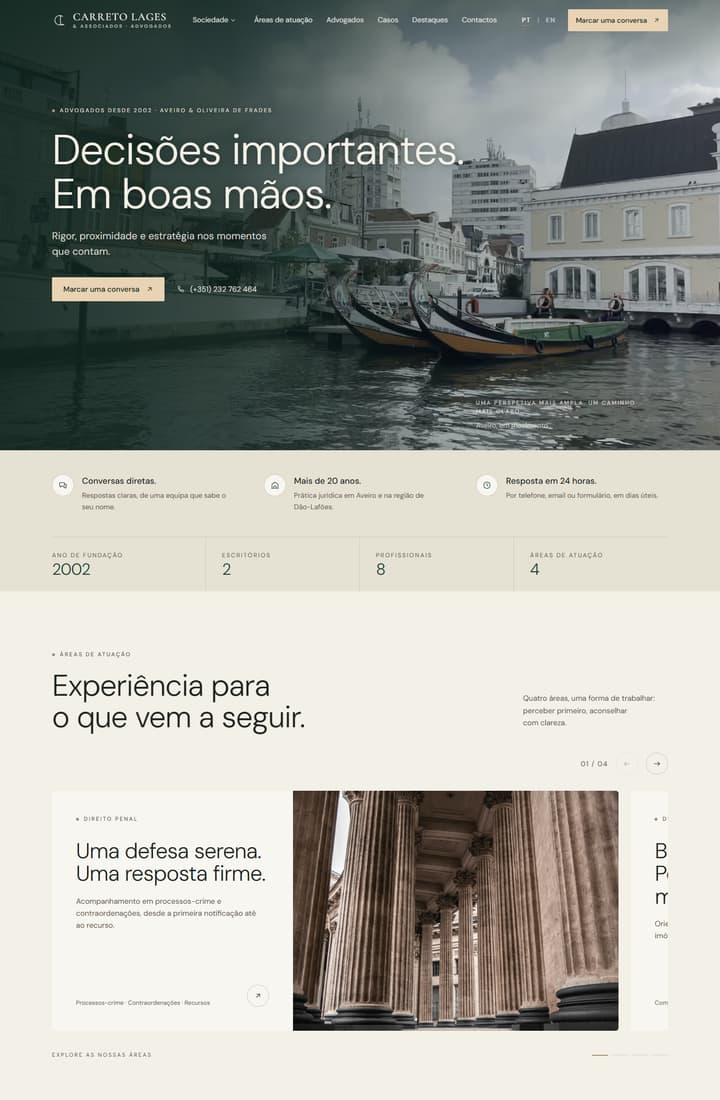
\includegraphics[width=0.62\textwidth]{screenshots/desktop/pt/home-1.jpg}\hfill
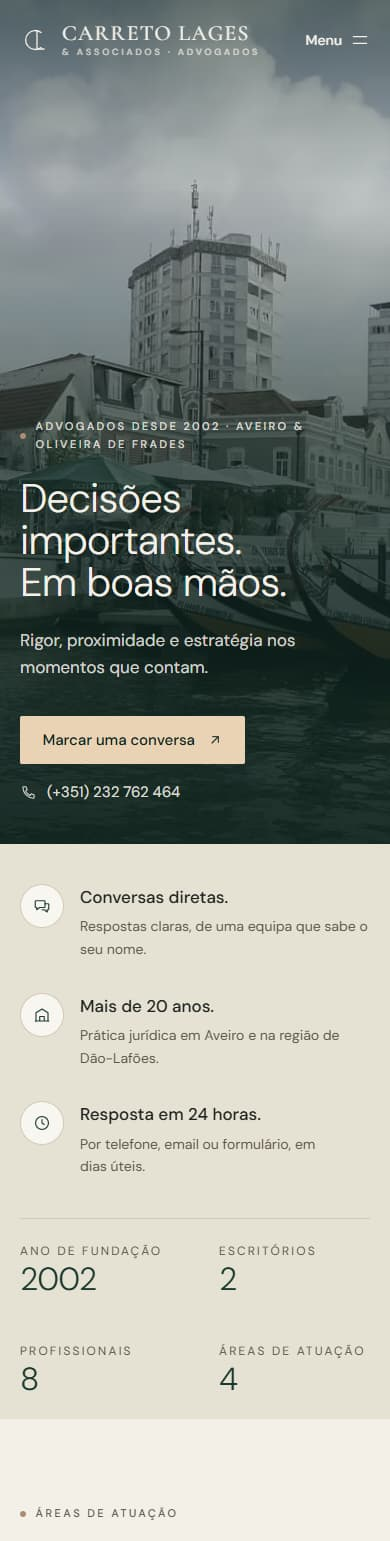
\includegraphics[width=0.3\textwidth]{screenshots/mobile/pt/home-1.jpg}
\end{center}

% =====================================================================
\section{Páginas interiores}
Todas as páginas secundárias abrem com um topo de imagem em largura total, a começar no topo da página, por
baixo do cabeçalho transparente, e terminam com um fio bronze em vez de cantos arredondados. Há dois tipos:
\begin{itemize}
  \item \textbf{Faixa com fotografia} (listas, contactos e páginas legais): fotografia com véu verde, título em baixo à esquerda e frase à direita, em estilo editorial.
  \item \textbf{Bloco verde} (Sociedade, História, Valores, Pro Bono, áreas, advogados, casos e artigos): etiqueta vertical em bronze no lado esquerdo, texto à esquerda e fotografia com uma moldura bronze deslocada. Na página de cada advogado a fotografia é o retrato; na História é o troféu do 20.º aniversário.
\end{itemize}
Sociedade (resumo, História, Perfil e Valores, Pro Bono), Áreas de atuação (índice e uma página por área,
com ``o que fazemos'', situações típicas, advogados da área e formulário com a área já escolhida),
Advogados (equipa por grupos e uma página por pessoa; quem ainda não tem fotografia aparece com as
iniciais), Casos práticos, Destaques (artigos), Contactos, Obrigado, página 404 e páginas legais
(Privacidade, Termos, Resolução de litígios, Cookies) marcadas ``Rascunho para revisão''. Todas terminam
com uma chamada para o contacto.

% =====================================================================
\section{Interações e estados}
Menu de telemóvel em gaveta que abre da esquerda e deixa uma faixa do site visível à direita (fecha ao tocar nessa faixa ou com Escape, e devolve o foco), submenu da Sociedade, cabeçalho
transparente sobre o vídeo que passa a marfim ao descer, seletor PT\,|\,EN que leva à mesma página na outra
língua, carrossel, separadores de situações (setas do teclado, Home/End), passos do processo, perguntas
frequentes, botão ``Copiar ligação'' nos artigos e casos, dois botões redondos discretos ``Ligar'' e ``Contactar'' no canto
inferior direito do telemóvel, que se escondem junto ao formulário. As capturas dos estados estão na secção de estados e interações.

% =====================================================================
\section{Versão inglesa}\label{sec:ingles}
Todo o conteúdo existe em inglês britânico, escrito para soar natural, em endereços próprios
(\texttt{/en/practice-areas/tax-law}, \texttt{/en/lawyers}, \ldots). Um teste automático percorre todas as
páginas inglesas e falha se encontrar texto de interface em português (nomes próprios excluídos). As páginas
legais em inglês indicam que prevalece a versão portuguesa.

% =====================================================================
\section{Vídeo de fundo}
O original (4K, 62\,MB) foi comprimido em três versões, sem som, com 15\,s em ciclo:
\begin{center}\resVideoTable\end{center}
\begin{itemize}
  \item A imagem de capa aparece primeiro com prioridade alta; o vídeo só é pedido depois de a página carregar e entra com uma transição suave.
  \item O browser recebe a versão do seu ecrã (vertical no telemóvel, 16:9 no resto).
  \item Sem vídeo para quem tem poupança de dados, movimento reduzido ou ligação lenta (2G/3G): fica só a imagem.
  \item Pausa automática fora do ecrã e em separadores escondidos; se o vídeo falhar, a imagem de capa mantém-se.
\end{itemize}
\begin{center}\resPosterTable\end{center}

% =====================================================================
\section{Formulário de contacto}
Campos: Nome*, Email*, Telefone, Área, Escritório preferido, Mensagem*, consentimento RGPD*. A validação é
partilhada entre o browser e o futuro servidor; os erros aparecem junto a cada campo, na língua da página,
sem apagar o que foi escrito, e são anunciados a leitores de ecrã. Proteção contra spam sem custos: campo
invisível, tempo mínimo de preenchimento e rejeição de campos inesperados. O gerador do email (para a fase
seguinte) escapa todo o texto do visitante e impede injeção no assunto.

\textbf{Nesta fase nada é enviado}: um envio válido apenas leva à página ``Obrigado'' (verificado por teste:
nenhum pedido de rede transporta os dados).

% =====================================================================
\section{Segurança e privacidade}
\subsection{Cabeçalhos HTTP}
\resHeadersTable

\subsection{Política de segurança de conteúdo (CSP)}
\resCspList
Sem \texttt{'unsafe-inline'} nem \texttt{'unsafe-eval'}. O único domínio externo permitido é o do Google
Maps, e só para o mapa embutido depois do clique.

\subsection{Verificações}
\begin{itemize}
  \item \textbf{Teste de segurança em todas as páginas} (computador e telemóvel): \resSecPassed{} verificações aprovadas, \resSecFailed{} falhadas --- cabeçalhos presentes, zero violações da CSP, zero erros na consola, zero pedidos a outros domínios e zero cookies.
  \item \textbf{Dependências}: \resAuditProd{} vulnerabilidades nas dependências de produção. Nas ferramentas de teste usadas localmente existem \resAuditDevModerate{} avisos moderados (\resAuditDevPackages), sem impacto no site publicado.
  \item \textbf{Segredos}: um teste confirma que nenhum ficheiro do repositório contém chaves ou ficheiros \texttt{.env}.
  \item \textbf{Privacidade}: sem cookies, sem estatísticas, fontes locais, mapa da Google só ao clicar --- não é necessário banner de cookies.
\end{itemize}

% =====================================================================
\section{Testes e qualidade}
\begin{itemize}
  \item \textbf{Testes unitários}: \resUnitPassed{} de \resUnitTotal{} aprovados (\resUnitFiles{} ficheiros) --- endereços, traduções, conteúdo, validação, vídeo, carrossel, separadores, dados estruturados, cabeçalhos, peso do JavaScript, segredos.
  \item \textbf{Testes de ponta a ponta} (Chrome, computador, telemóvel e sem JavaScript): \resEtoePassed{} aprovados, \resEtoeFailed{} falhados, \resEtoeSkipped{} não aplicáveis ao perfil.
  \item \textbf{Acessibilidade (axe, WCAG 2.2 AA)}: \resAxeRuns{} análises (todas as páginas, computador e telemóvel); \resAxeSerious{} problemas graves ou críticos; outros avisos: \resAxeOther{} (\resAxeRules).
  \item \textbf{Ecrãs de 360\,px}: nenhuma página com \textit{scroll} horizontal nem botões ou títulos cortados.
  \item \textbf{Ligações}: \resLinksChecked{} verificadas, \resLinksBroken{} partidas.
  \item \textbf{JavaScript por página}: entre \resJsMin{} e \resJsMax{} (gzip), em \resJsPages{} páginas; limite 50\,KB.
\end{itemize}

\subsection{Lighthouse (telemóvel, 4G simulado, mediana de 3 execuções)}
\begin{center}\resLighthouseTable\end{center}
Medido numa versão sem \texttt{noindex} (a pré-visualização tem \texttt{noindex} de propósito, o que baixaria
a nota de SEO).

\subsection{JavaScript por página}
\begin{center}\resJsTable\end{center}

% =====================================================================
\section{Publicação de teste}
O site está publicado para revisão em \textbf{\url{https://carretolages.pages.dev}} (Cloudflare Pages, plano
gratuito; conta sem subscrições nem método de pagamento --- verificado antes e depois da publicação).
\begin{itemize}
  \item Envio direto da pasta gerada (290 ficheiros), sem ligação ao GitHub e sem funções de servidor.
  \item Todas as páginas têm \texttt{noindex} e o cabeçalho \texttt{X-Robots-Tag: noindex, nofollow}: o site não aparece no Google.
  \item Os cabeçalhos de segurança da secção anterior foram confirmados no endereço público; páginas inexistentes devolvem 404 (portuguesa ou inglesa).
  \item Os testes de rotas e de segurança foram repetidos contra o site publicado: \textbf{\resLivePassed{} aprovados, \resLiveFailed{} falhados}.
\end{itemize}

% =====================================================================
\section{Decisões tomadas durante a construção}
\begin{longtable}{p{3.2cm}p{6.4cm}p{5.4cm}}
\toprule
\textbf{Tema} & \textbf{Decisão} & \textbf{Porquê} \\
\midrule
\endhead
Endereços & As páginas são servidas sem ``.html'' nem barra final (ex.: /advogados); o inglês fica em /en. & É o formato que a Cloudflare Pages serve sem redireções e mantém os endereços curtos. \\
Conteúdo & O conteúdo vive em ficheiros JSON validados (Zod) com campos PT/EN lado a lado, organizados como os futuros modelos do Sanity. & Permite testar tudo automaticamente e ligar o Sanity mais tarde sem mudar o desenho. \\
Conteúdo & Textos longos (artigos, páginas legais) guardados como blocos simples (parágrafo, título, lista). & Corresponde ao formato de texto rico do Sanity e evita dependências extra. \\
Conteúdo & Moradas completas dos escritórios marcadas ``a confirmar''; biografias limitadas a factos conhecidos. & Não inventar informação sobre o escritório nem sobre as pessoas. \\
Vídeo & Compressão com qualidade constante e teto de débito; o MP4 vem antes do WebM. & A textura da água fazia o WebM ultrapassar o limite de 2,5 MB; com o teto, o MP4 ficou mais leve. \\
Vídeo & Imagem de capa própria para telemóvel (recorte vertical) e capas de reserva limitadas a 100 KB. & A capa tem de coincidir com o vídeo vertical e aparecer depressa em 4G. \\
Vídeo & O botão de pausa do vídeo deixou de estar visível (pedido do cliente); aparece apenas quando alcançado com a tecla Tab. & Mantém a conformidade com WCAG 2.2.2 (forma de parar conteúdo em movimento) sem ocupar espaço visual. \\
Imagens & Imagens de banco ligeiramente dessaturadas por CSS. & Integram-se na paleta calma sem reprocessar ficheiros que vão ser substituídos. \\
Navegação & O menu completo aparece a partir de 1280 px; abaixo disso usa-se o botão Menu e a barra fixa Ligar/Contactar. & A 1024 px o menu completo com o botão não cabia sem partir linhas. \\
Rodapé & Rodapé claro (areia), como na referência Alden \& Vale. & Mantém o tom calmo; o verde escuro fica reservado ao topo e às chamadas para ação. \\
Situações & Separadores (ARIA tabs) em ecrãs largos e acordeão no telemóvel; sem JavaScript tudo fica visível. & Cada formato funciona melhor no seu ecrã e nada se perde sem JavaScript. \\
Formulário & Escritório preferido escolhido com botões (``chips''), por omissão ``Indiferente''. & Menos toques no telemóvel. \\
Formulário & Aviso ``sem JavaScript'' mostrado por CSS (@media scripting: none) em vez de ser removido por script. & Remover o aviso depois de carregar fazia a página saltar (CLS 0,106). \\
Mapas & Mapa ilustrado (SVG) desenhado no próprio site até ao clique; só então carrega o Google Maps. & Nenhum pedido à Google nem cookies antes da ação do visitante. \\
Coleções vazias & Casos, testemunhos e destaques sem conteúdo desaparecem da página inicial, do menu e do mapa do site. & Requisito do documento; nesta fase aparecem com o selo ``Exemplo ilustrativo''. \\
Segurança & Política de segurança de conteúdo (CSP) só por cabeçalho HTTP, sem 'unsafe-inline' nem 'unsafe-eval'. & O site não tem scripts nem estilos embutidos, por isso a política mais restrita funciona. \\
Segurança & A biblioteca de validação (Zod) corre em modo ``jitless''. & Os testes mostraram que ela tentava usar eval, que a CSP bloqueia — e bem. \\
Segurança & Auditoria de dependências bloqueia apenas dependências de produção (0 vulnerabilidades). & As 6 vulnerabilidades moderadas estão só em ferramentas de teste usadas localmente. \\
Desempenho & Pré-carregamento da letra DM Sans; a letra do logótipo carrega normalmente. & Evita saltos de texto (CLS) sem roubar largura de banda à imagem de capa em 4G. \\
Testes & Lighthouse com pedido de aquecimento e mediana de 3 execuções por página. & Execuções únicas a frio davam valores anómalos (2,9 s) que não representam o site. \\
Testes & Playwright e Lighthouse usam o Google Chrome já instalado. & Evita descarregar 150 MB de browsers de teste. \\
Testes & Na versão inglesa, nomes próprios (``Sociedade de Advogados'', ``Ordem dos Advogados'', linha do logótipo) não contam como texto português. & São nomes, não texto de interface por traduzir. \\
Telemóvel & Os botões Ligar/Contactar passaram de barra em largura total a dois botões redondos no canto inferior direito. & Pedido do cliente: menos chamativos e sem ocupar a parte de baixo do ecrã. \\
Páginas secundárias & Topo de imagem em largura total, do topo da página, com fio bronze no fundo; faixa editorial com fotografia ou bloco verde com etiqueta vertical e moldura deslocada. & Pedido do cliente (topos mais bonitos), sem copiar o estilo da referência e sem margens brancas no topo e nos lados. \\
Advogados & Cargo e nome escritos dentro da fotografia, sobre gradiente escuro. & Pedido do cliente, inspirado na referência. \\
20 anos & Nova secção na página inicial com o troféu do 20.º aniversário; o troféu é também a imagem do topo da História. & Pedido do cliente; o texto usa só factos conhecidos (fundação em 2002, 20 anos em 2022). \\
Telemóvel & O menu passou a gaveta que abre da esquerda, com uma margem de 3,5 rem à direita onde o site continua visível; tocar nessa margem fecha o menu. & Pedido do cliente. \\
Imagens & As caixas de imagem com proporção fixa cortam o excesso (overflow: hidden). & Sem isso, a fotografia (3:2) fazia a caixa (16:9) crescer quando carregava durante o scroll no telemóvel — problema reportado pelo cliente nos Destaques. \\
\bottomrule
\end{longtable}


% =====================================================================
\section{Pendentes para a versão final}\label{sec:pendentes}
\begin{enumerate}
  \item Moradas completas, coordenadas e telefone de cada escritório.
  \item Email que recebe os pedidos (presumido \texttt{geral@carretolages.com}).
  \item Dados legais para as páginas legais: denominação social, NIPC, sede e contacto RGPD; revisão dos rascunhos.
  \item Validação deontológica dos casos práticos e testemunhos reais (os atuais são exemplos).
  \item Fotografias dos cinco profissionais sem retrato e, mais tarde, fotografias próprias dos escritórios.
  \item Revisão dos textos em português e inglês pelo escritório.
  \item Titularidade das contas (domínio novo, Cloudflare, Resend, Sanity) e manutenção após a entrega.
  \item Fase seguinte: envio real do formulário (Resend), painel Sanity, domínio novo e retirar o \texttt{noindex}.
\end{enumerate}

% =====================================================================
\section{Créditos das imagens}
\begin{longtable}{p{4cm}p{4cm}p{6.8cm}}
\toprule
\textbf{Imagem} & \textbf{Autor} & \textbf{Origem} \\
\midrule
\endhead
\texttt{aveiro-canal} & Luís Cardoso & \url{https://unsplash.com/photos/QmvnZ_A5So4} (Unsplash License) \\
\texttt{countryside-hills} & Filipe Nobre & \url{https://unsplash.com/photos/sDrCPS3V4a0} (Unsplash License) \\
\texttt{architecture-columns} & Denis Vdovin & \url{https://unsplash.com/photos/qF6C1UDXyN0} (Unsplash License) \\
\texttt{modern-house} & George Barros & \url{https://unsplash.com/photos/t4FMbSdmeR0} (Unsplash License) \\
\texttt{desk-documents} & 2H Media & \url{https://unsplash.com/photos/spScdgWY-_c} (Unsplash License) \\
\texttt{glass-facade} & Christian Ladewig & \url{https://unsplash.com/photos/T0iFfJw-rB0} (Unsplash License) \\
\texttt{office-corridor} & Craig Lovelidge & \url{https://unsplash.com/photos/-2Khf-1qoCA} (Unsplash License) \\
\texttt{meeting-room} & Craig Lovelidge & \url{https://unsplash.com/photos/s-KphF10sWM} (Unsplash License) \\
\texttt{library-books} & Thomas Bormans & \url{https://unsplash.com/photos/IHQHXj3jv6E} (Unsplash License) \\
\texttt{conversation-table} & charlesdeluvio & \url{https://unsplash.com/photos/rRWiVQzLm7k} (Unsplash License) \\
\bottomrule
\end{longtable}


% =====================================================================
\clearpage
\section{Páginas — versão portuguesa}
\needspace{8\baselineskip}
\subsection*{Decisões importantes. Em boas mãos.}
\addcontentsline{toc}{subsection}{Decisões importantes. Em boas mãos. (\texttt{/})}
\noindent{\small\color{tintasuave}\texttt{/}}\par\smallskip
\noindent{\footnotesize Computador (1440\,px)}\par\smallskip
\noindent 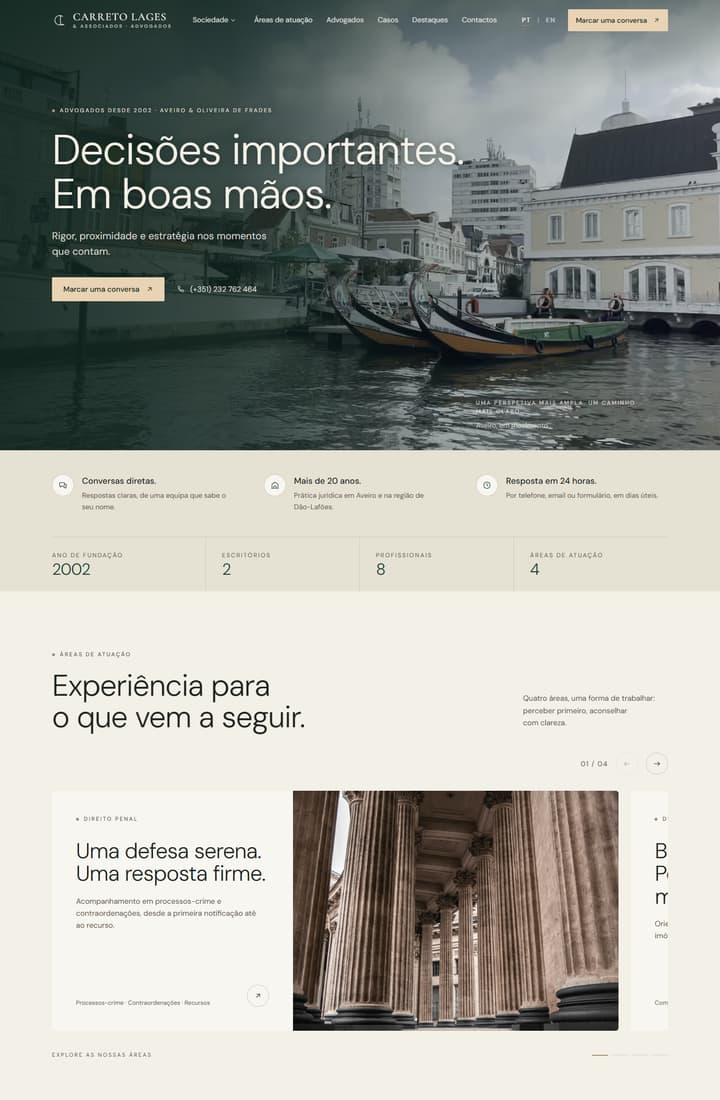
\includegraphics[width=0.485\textwidth]{screenshots/desktop/pt/home-1.jpg}\hspace{0.012\textwidth}
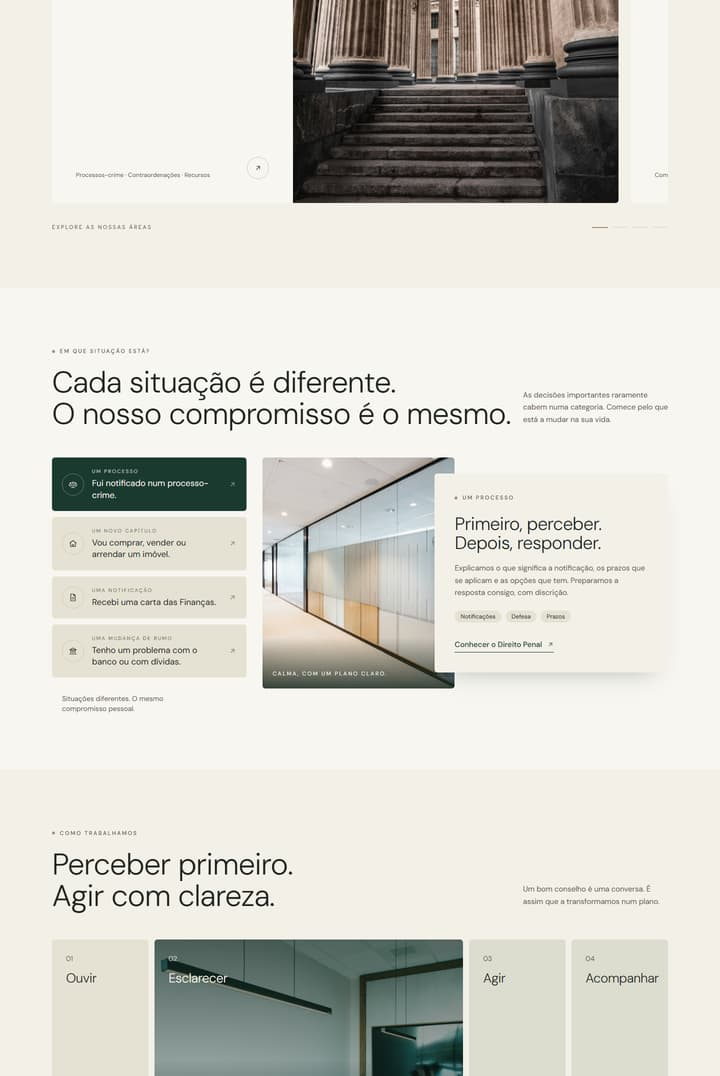
\includegraphics[width=0.485\textwidth]{screenshots/desktop/pt/home-2.jpg}\par\medskip
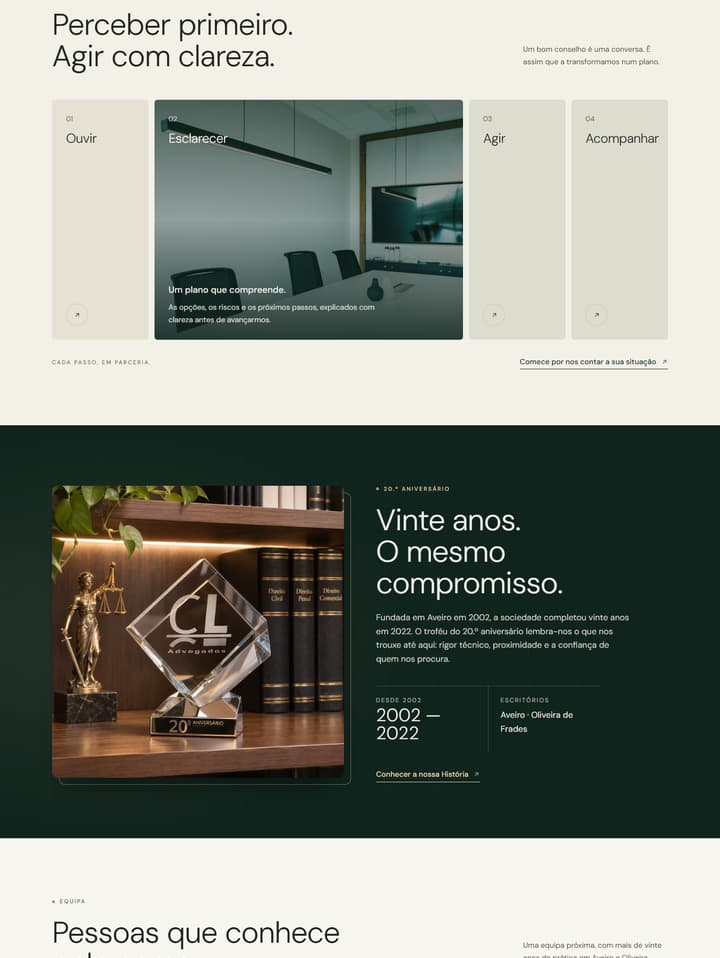
\includegraphics[width=0.485\textwidth]{screenshots/desktop/pt/home-3.jpg}\hspace{0.012\textwidth}
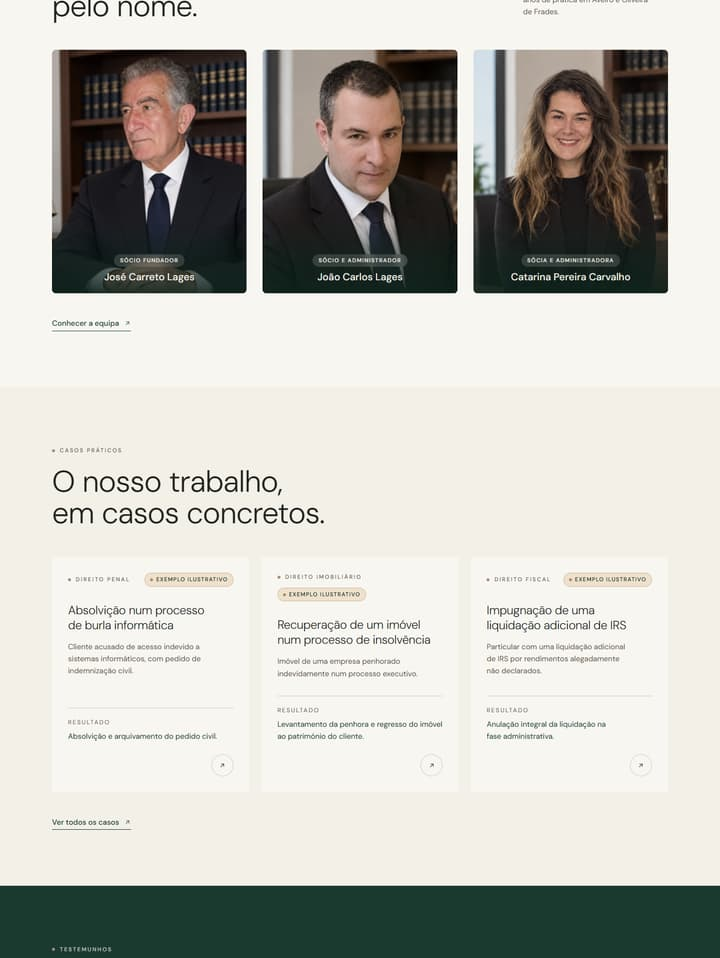
\includegraphics[width=0.485\textwidth]{screenshots/desktop/pt/home-4.jpg}\par\medskip
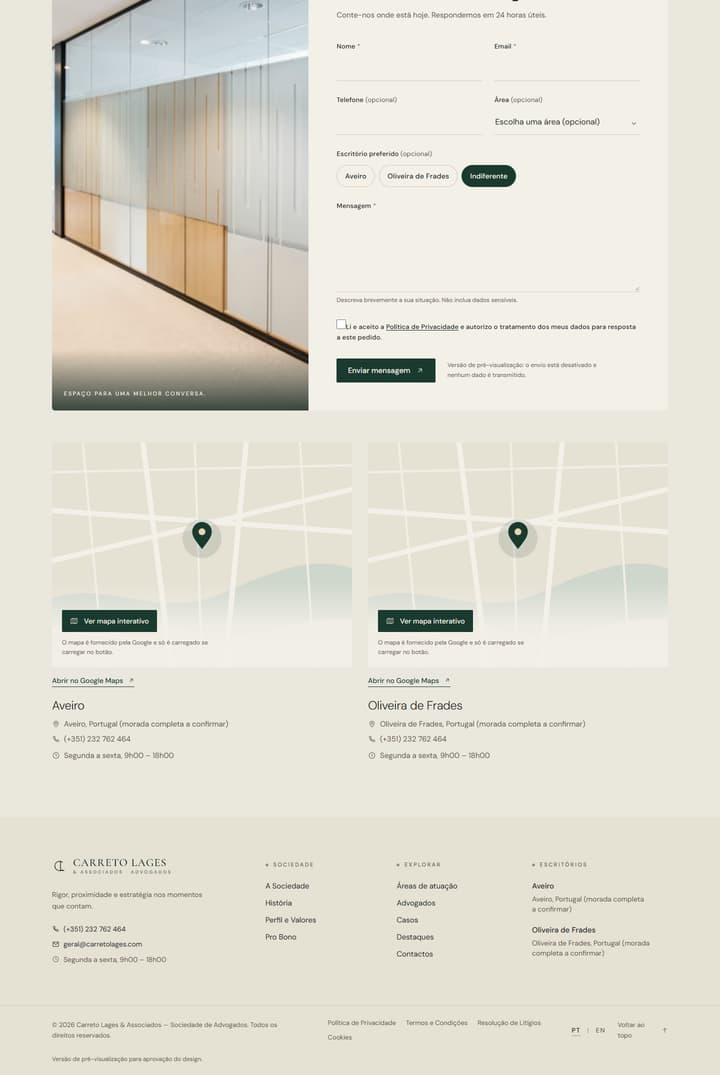
\includegraphics[width=0.485\textwidth]{screenshots/desktop/pt/home-5.jpg}\par\medskip
\noindent{\footnotesize Telemóvel (390\,px)}\par\smallskip
\noindent 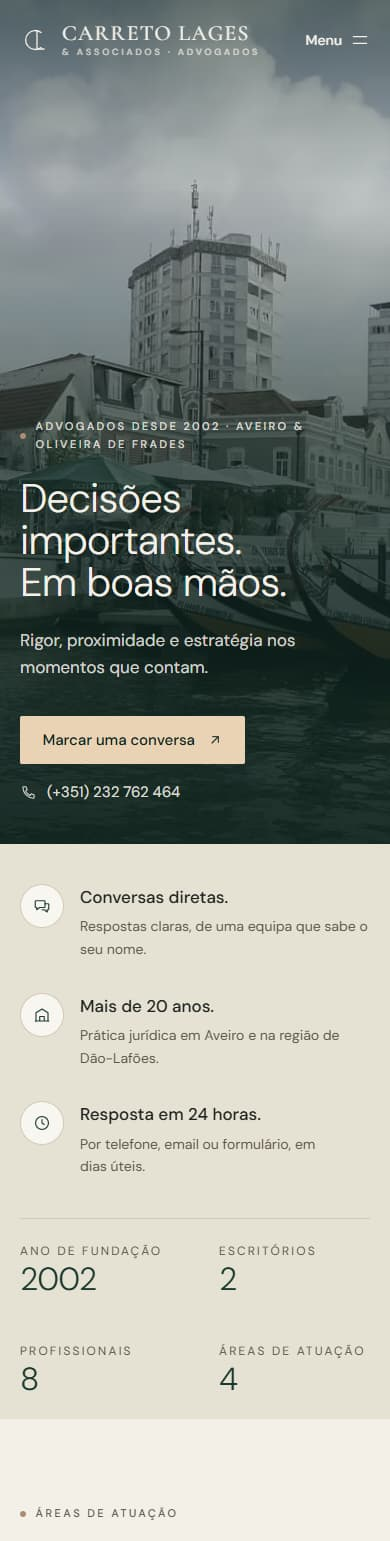
\includegraphics[width=0.235\textwidth]{screenshots/mobile/pt/home-1.jpg}\hspace{0.012\textwidth}
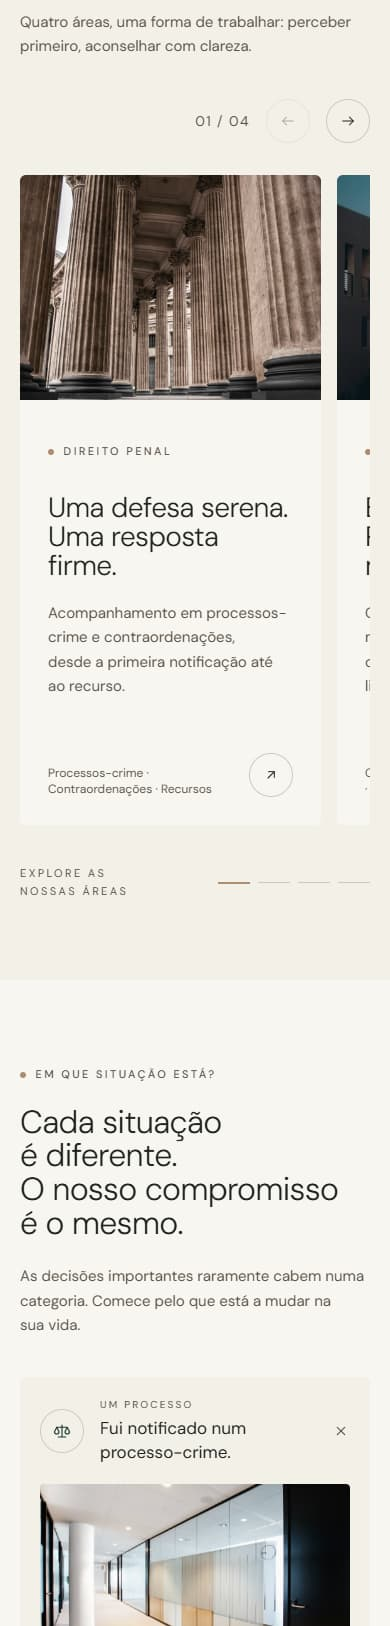
\includegraphics[width=0.235\textwidth]{screenshots/mobile/pt/home-2.jpg}\hspace{0.012\textwidth}
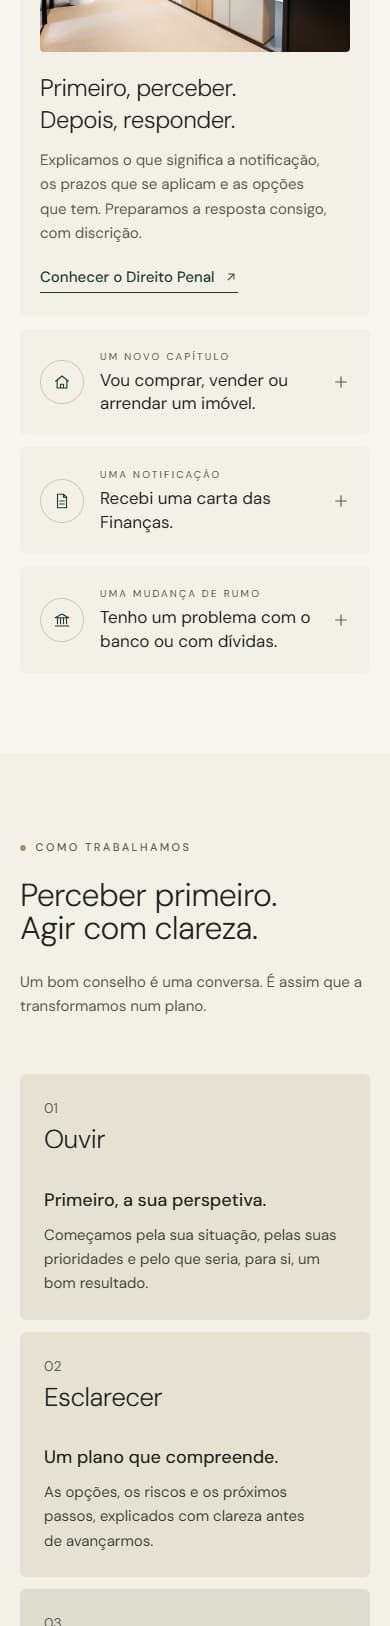
\includegraphics[width=0.235\textwidth]{screenshots/mobile/pt/home-3.jpg}\hspace{0.012\textwidth}
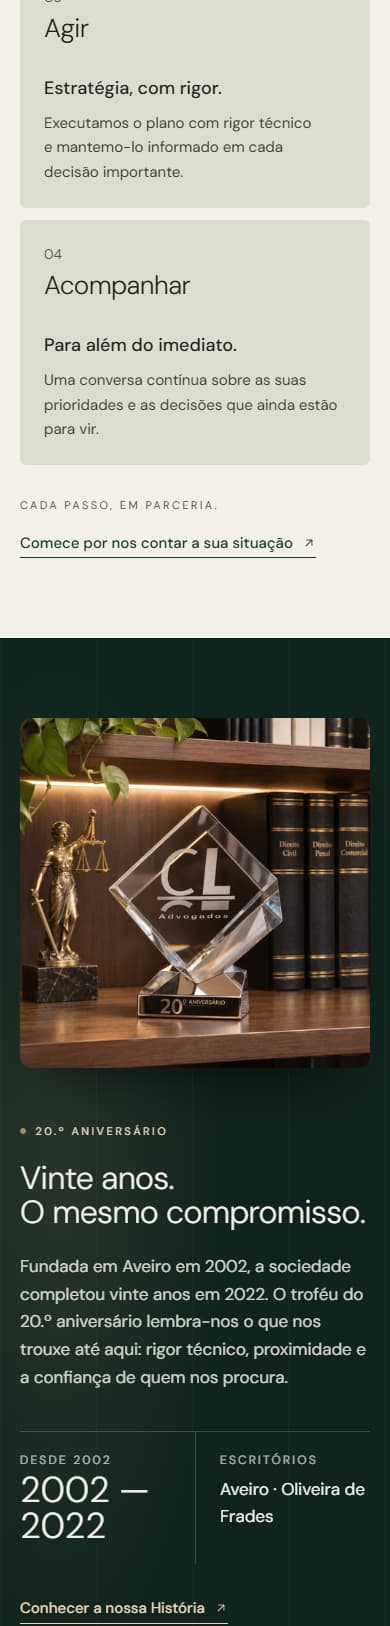
\includegraphics[width=0.235\textwidth]{screenshots/mobile/pt/home-4.jpg}\par\medskip
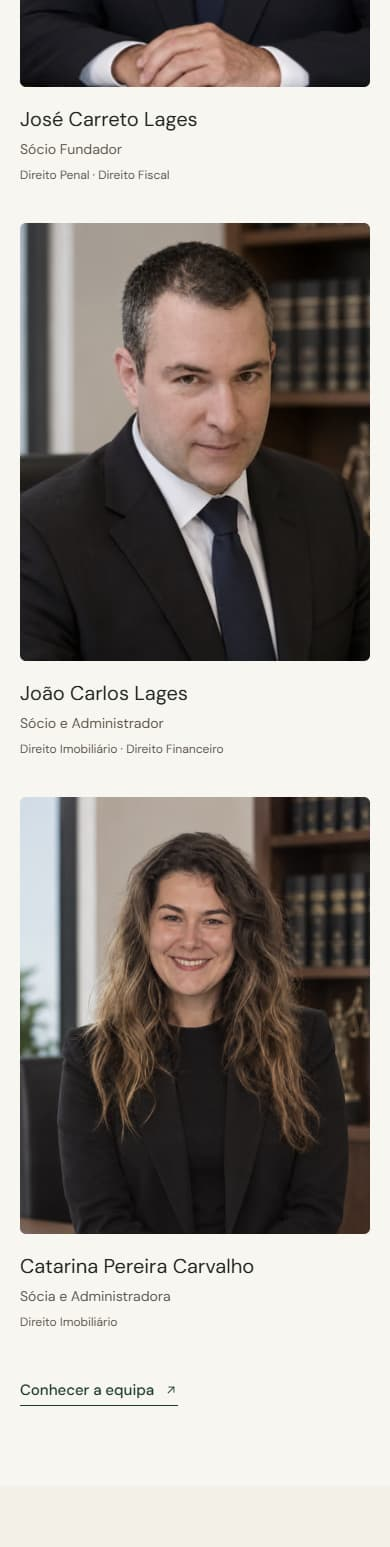
\includegraphics[width=0.235\textwidth]{screenshots/mobile/pt/home-5.jpg}\hspace{0.012\textwidth}
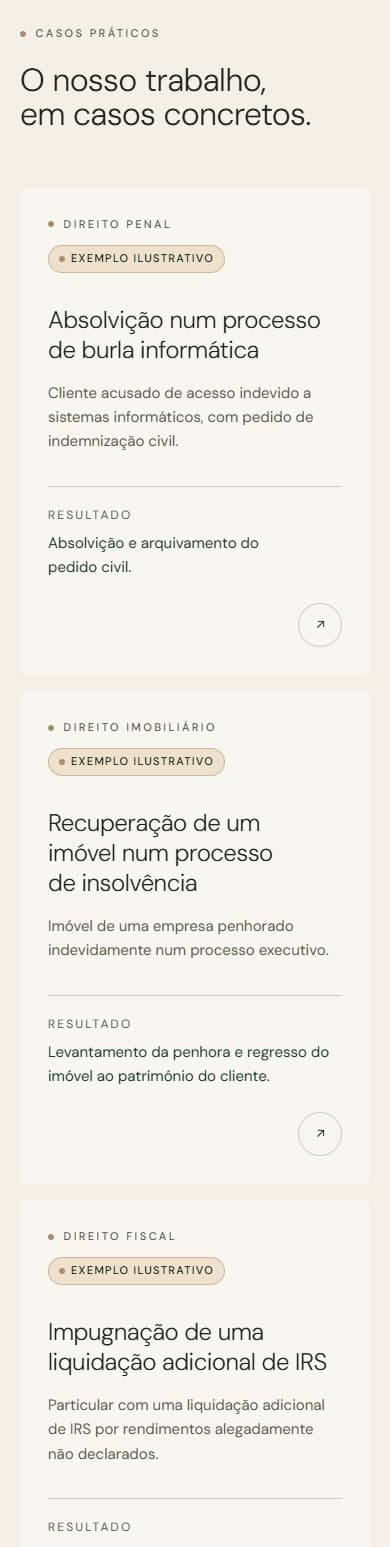
\includegraphics[width=0.235\textwidth]{screenshots/mobile/pt/home-6.jpg}\hspace{0.012\textwidth}
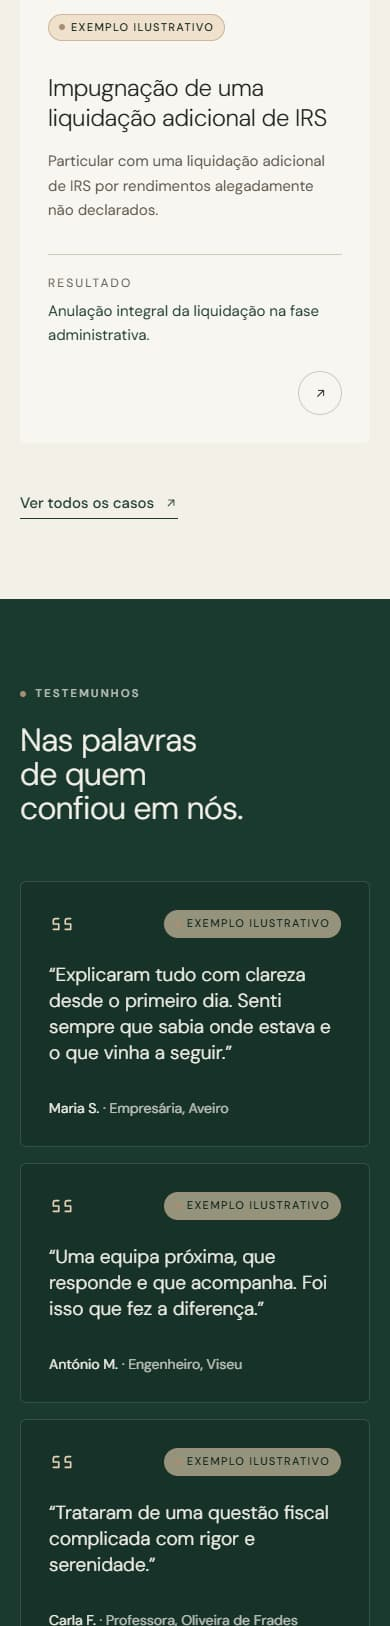
\includegraphics[width=0.235\textwidth]{screenshots/mobile/pt/home-7.jpg}\hspace{0.012\textwidth}
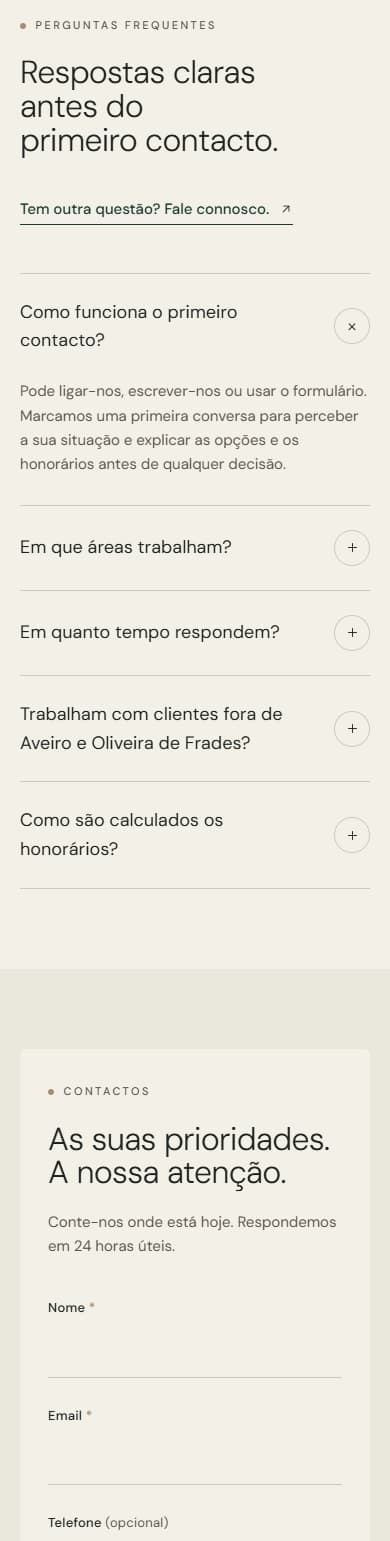
\includegraphics[width=0.235\textwidth]{screenshots/mobile/pt/home-8.jpg}\par\medskip
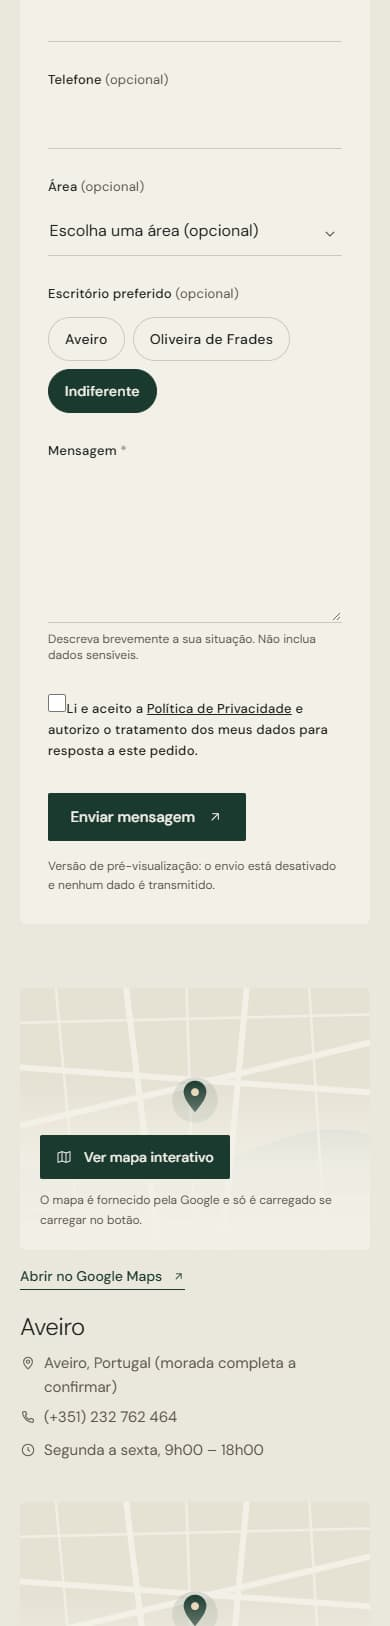
\includegraphics[width=0.235\textwidth]{screenshots/mobile/pt/home-9.jpg}\hspace{0.012\textwidth}
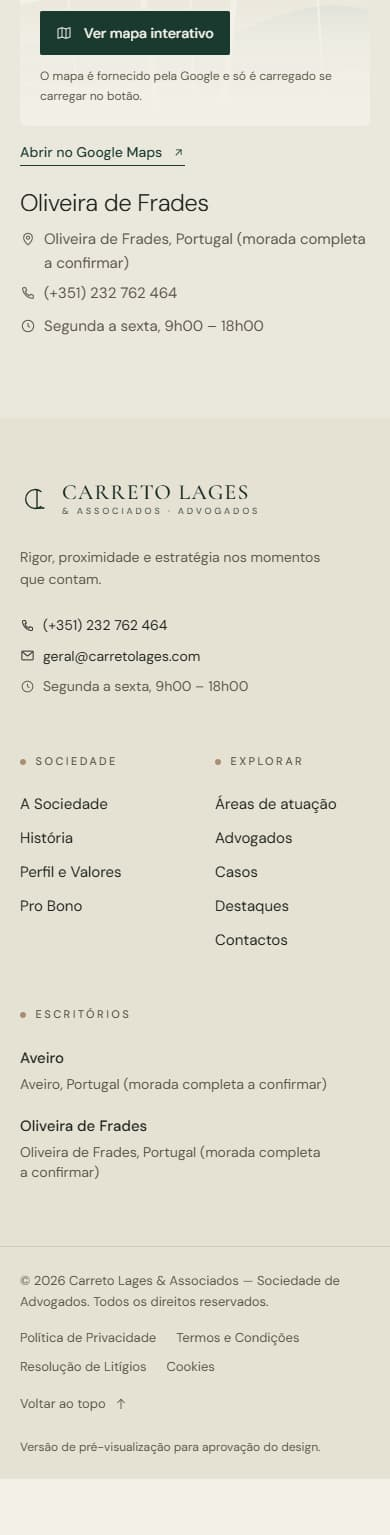
\includegraphics[width=0.235\textwidth]{screenshots/mobile/pt/home-10.jpg}\par\medskip
\bigskip
\needspace{8\baselineskip}
\subsection*{Esta página não existe.}
\addcontentsline{toc}{subsection}{Esta página não existe. (\texttt{/404})}
\noindent{\small\color{tintasuave}\texttt{/404}}\par\smallskip
\noindent{\footnotesize Computador (1440\,px)}\par\smallskip
\noindent 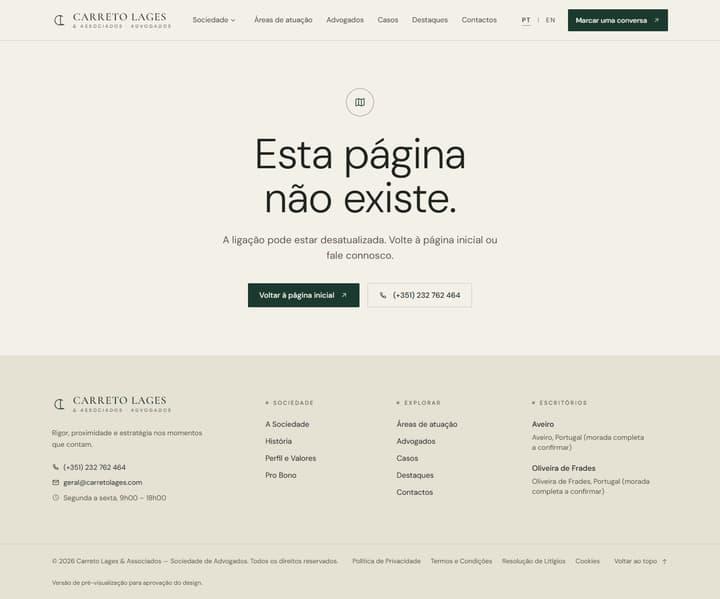
\includegraphics[width=0.485\textwidth]{screenshots/desktop/pt/404.jpg}\par\medskip
\noindent{\footnotesize Telemóvel (390\,px)}\par\smallskip
\noindent 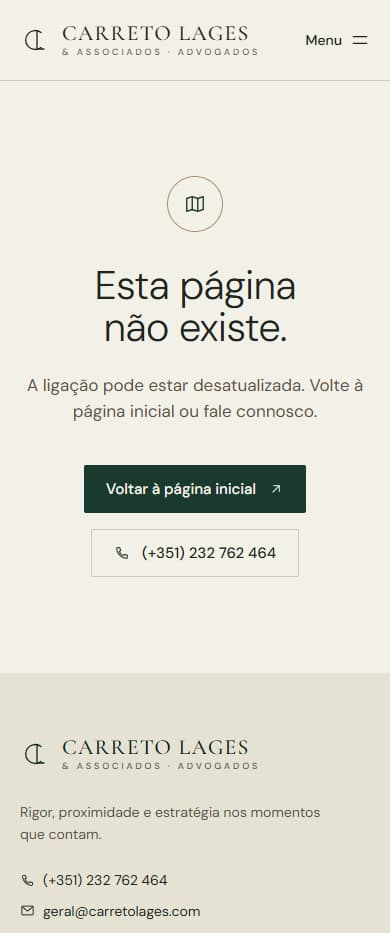
\includegraphics[width=0.235\textwidth]{screenshots/mobile/pt/404-1.jpg}\hspace{0.012\textwidth}
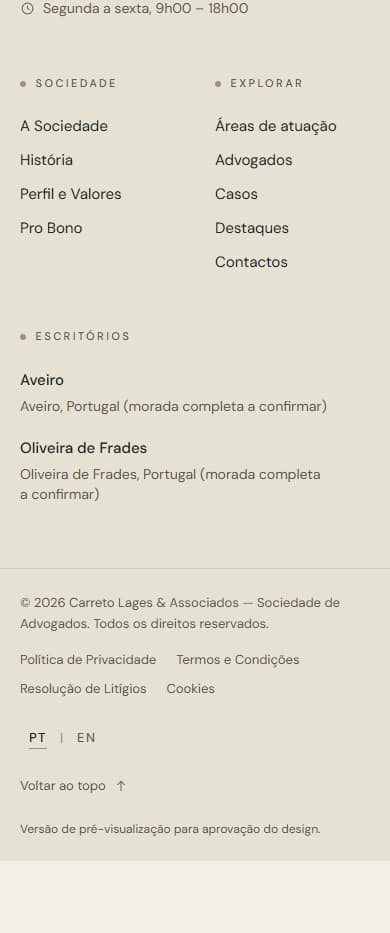
\includegraphics[width=0.235\textwidth]{screenshots/mobile/pt/404-2.jpg}\par\medskip
\bigskip
\needspace{8\baselineskip}
\subsection*{Pessoas que conhece pelo nome.}
\addcontentsline{toc}{subsection}{Pessoas que conhece pelo nome. (\texttt{/advogados})}
\noindent{\small\color{tintasuave}\texttt{/advogados}}\par\smallskip
\noindent{\footnotesize Computador (1440\,px)}\par\smallskip
\noindent 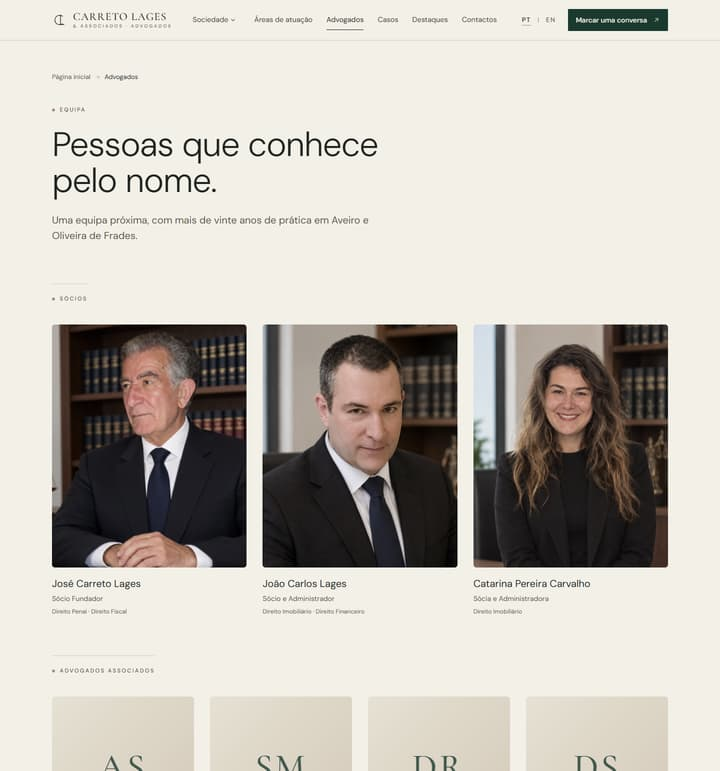
\includegraphics[width=0.485\textwidth]{screenshots/desktop/pt/advogados-1.jpg}\hspace{0.012\textwidth}
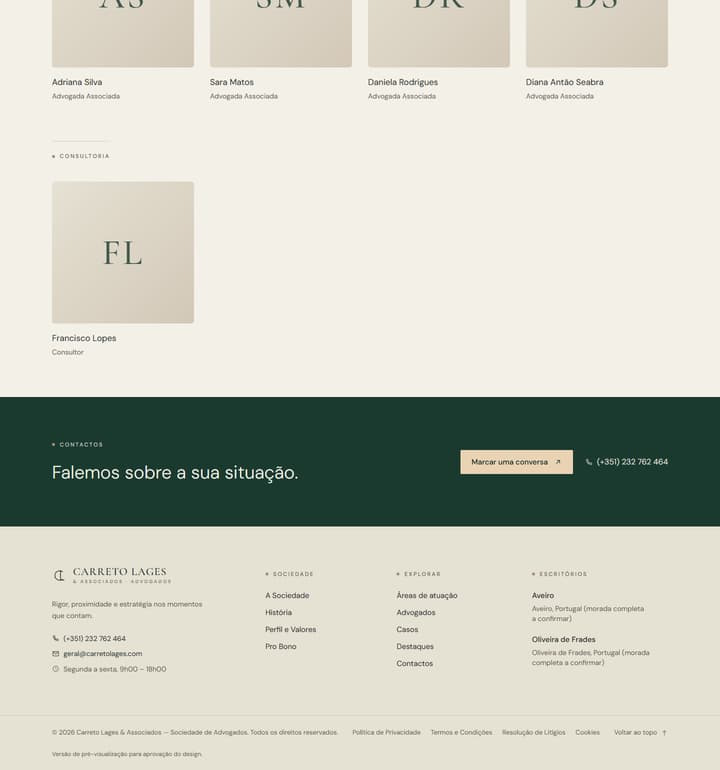
\includegraphics[width=0.485\textwidth]{screenshots/desktop/pt/advogados-2.jpg}\par\medskip
\noindent{\footnotesize Telemóvel (390\,px)}\par\smallskip
\noindent 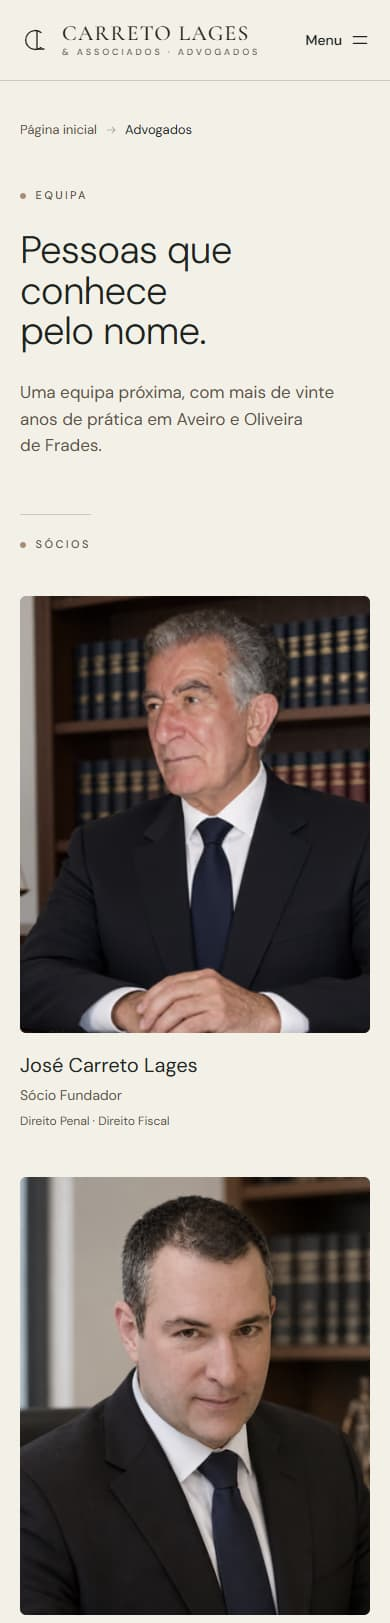
\includegraphics[width=0.235\textwidth]{screenshots/mobile/pt/advogados-1.jpg}\hspace{0.012\textwidth}

\includegraphics[width=0.235\textwidth]{screenshots/mobile/pt/advogados-2.jpg}\hspace{0.012\textwidth}
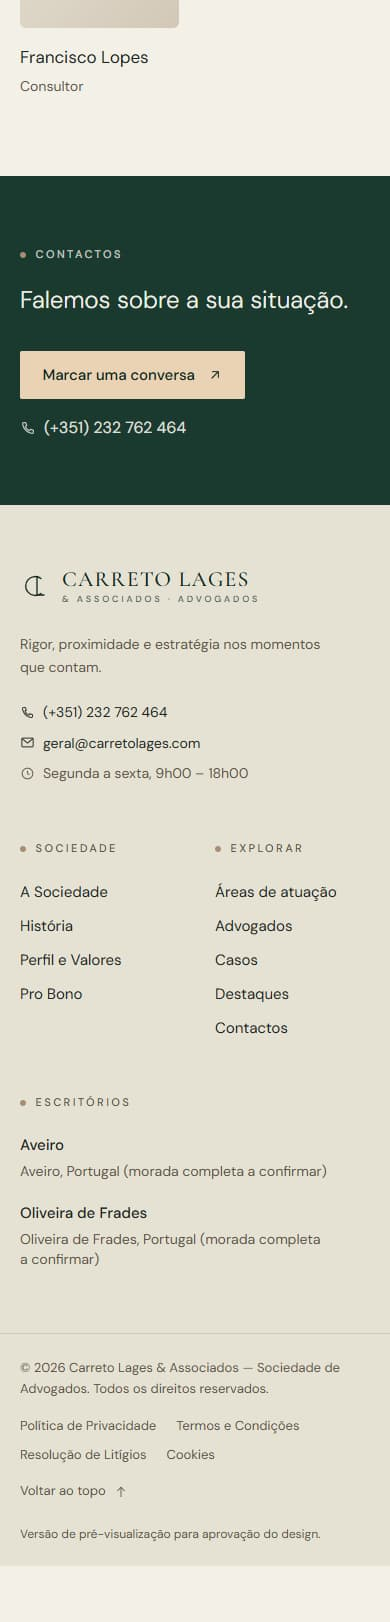
\includegraphics[width=0.235\textwidth]{screenshots/mobile/pt/advogados-3.jpg}\par\medskip
\bigskip
\needspace{8\baselineskip}
\subsection*{Adriana Silva}
\addcontentsline{toc}{subsection}{Adriana Silva (\texttt{/advogados/adriana-silva})}
\noindent{\small\color{tintasuave}\texttt{/advogados/adriana-silva}}\par\smallskip
\noindent{\footnotesize Computador (1440\,px)}\par\smallskip
\noindent 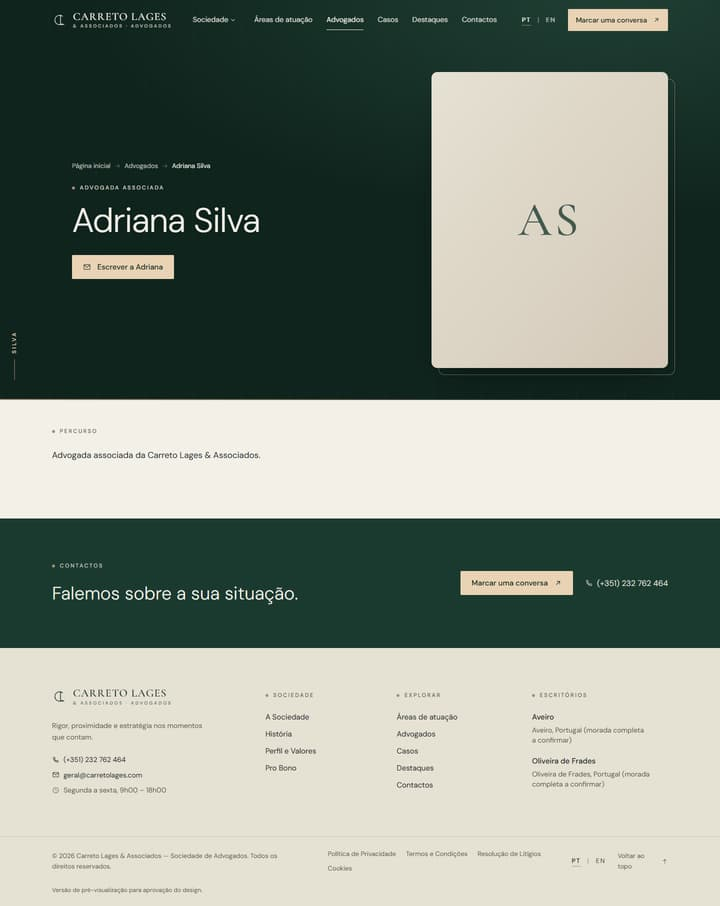
\includegraphics[width=0.485\textwidth]{screenshots/desktop/pt/advogados--adriana-silva.jpg}\par\medskip
\noindent{\footnotesize Telemóvel (390\,px)}\par\smallskip
\noindent 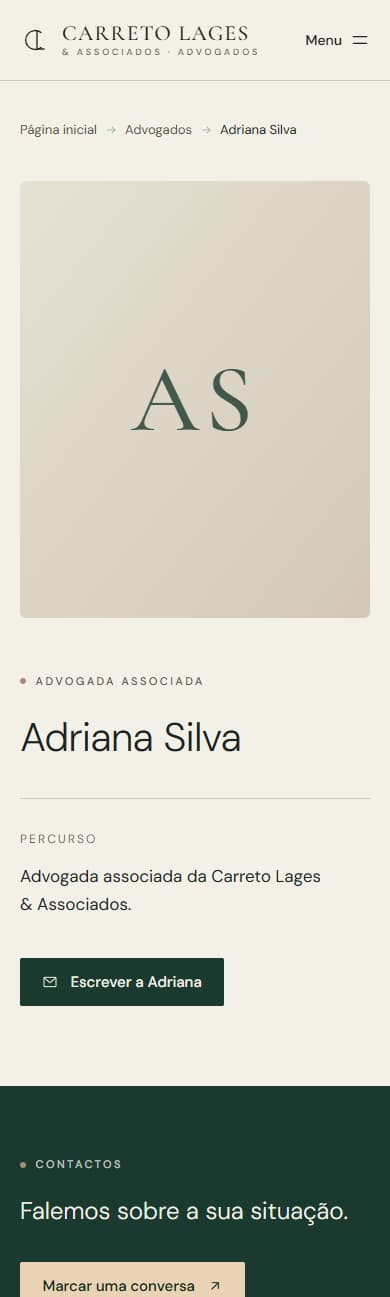
\includegraphics[width=0.235\textwidth]{screenshots/mobile/pt/advogados--adriana-silva-1.jpg}\hspace{0.012\textwidth}
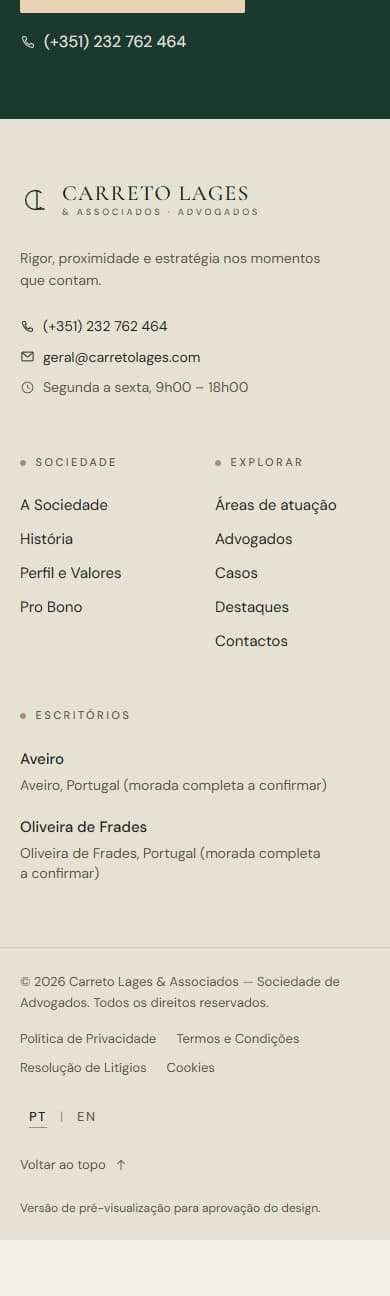
\includegraphics[width=0.235\textwidth]{screenshots/mobile/pt/advogados--adriana-silva-2.jpg}\par\medskip
\bigskip
\needspace{8\baselineskip}
\subsection*{Catarina Pereira Carvalho}
\addcontentsline{toc}{subsection}{Catarina Pereira Carvalho (\texttt{/advogados/catarina-pereira-carvalho})}
\noindent{\small\color{tintasuave}\texttt{/advogados/catarina-pereira-carvalho}}\par\smallskip
\noindent{\footnotesize Computador (1440\,px)}\par\smallskip
\noindent 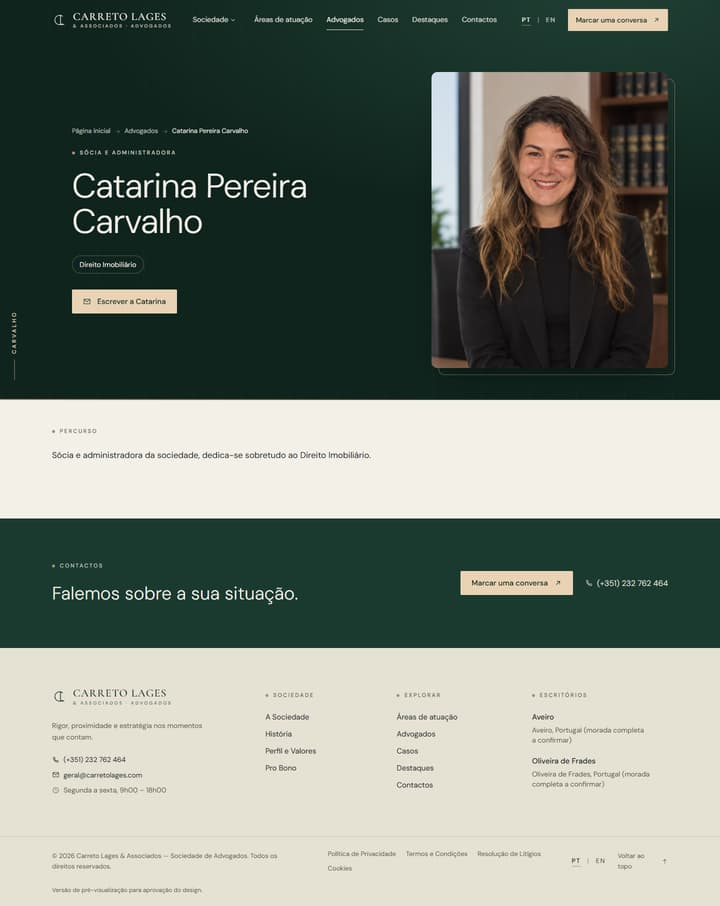
\includegraphics[width=0.485\textwidth]{screenshots/desktop/pt/advogados--catarina-pereira-carvalho.jpg}\par\medskip
\noindent{\footnotesize Telemóvel (390\,px)}\par\smallskip
\noindent 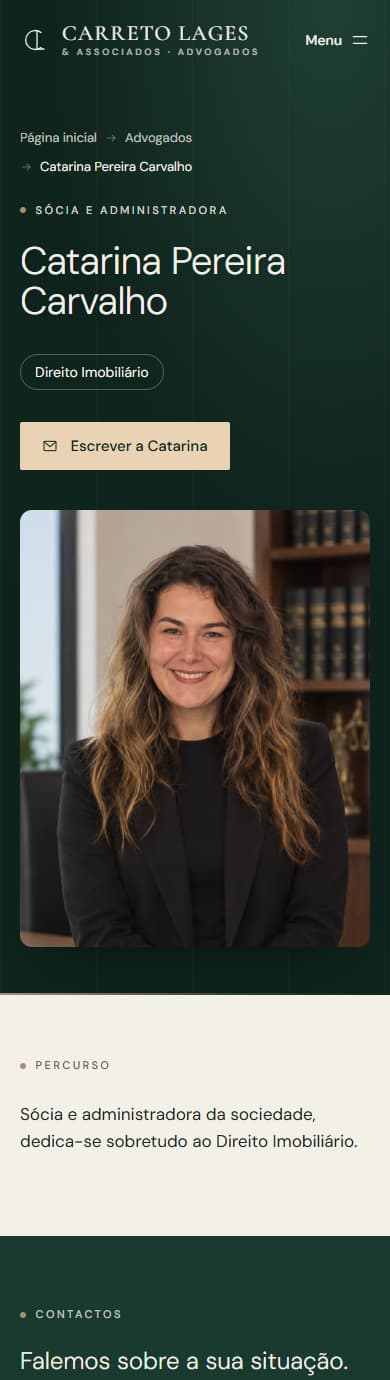
\includegraphics[width=0.235\textwidth]{screenshots/mobile/pt/advogados--catarina-pereira-carvalho-1.jpg}\hspace{0.012\textwidth}
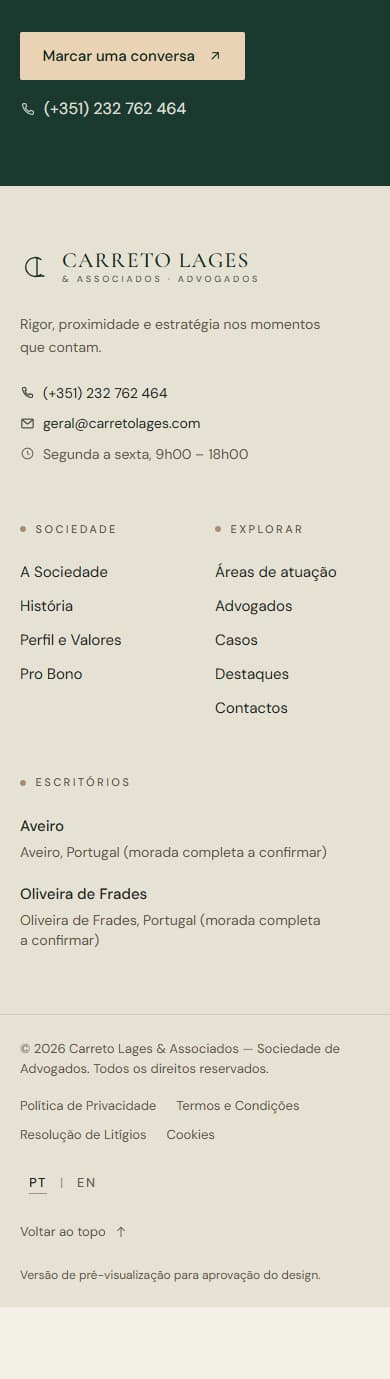
\includegraphics[width=0.235\textwidth]{screenshots/mobile/pt/advogados--catarina-pereira-carvalho-2.jpg}\par\medskip
\bigskip
\needspace{8\baselineskip}
\subsection*{Daniela Rodrigues}
\addcontentsline{toc}{subsection}{Daniela Rodrigues (\texttt{/advogados/daniela-rodrigues})}
\noindent{\small\color{tintasuave}\texttt{/advogados/daniela-rodrigues}}\par\smallskip
\noindent{\footnotesize Computador (1440\,px)}\par\smallskip
\noindent 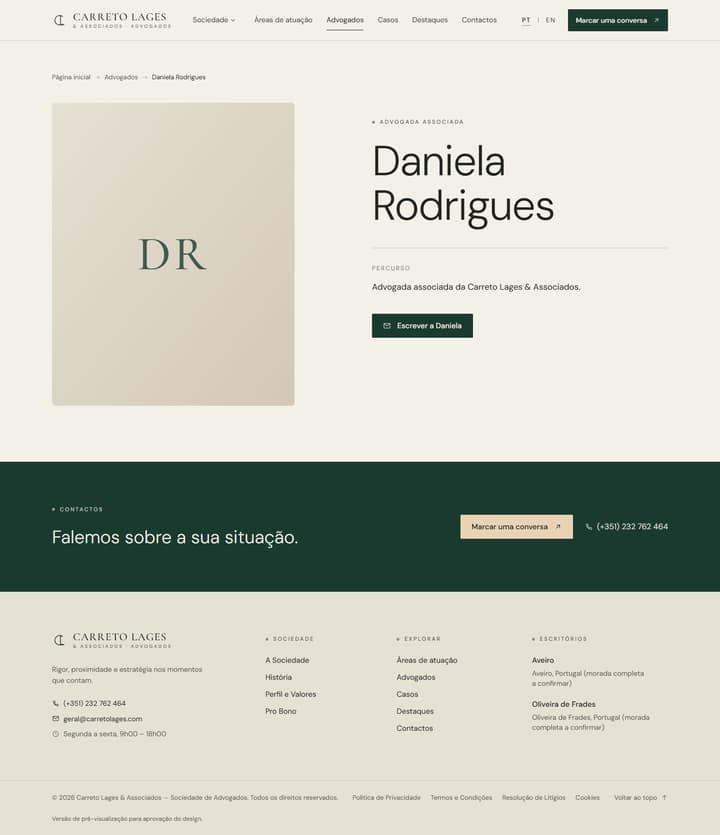
\includegraphics[width=0.485\textwidth]{screenshots/desktop/pt/advogados--daniela-rodrigues.jpg}\par\medskip
\noindent{\footnotesize Telemóvel (390\,px)}\par\smallskip
\noindent 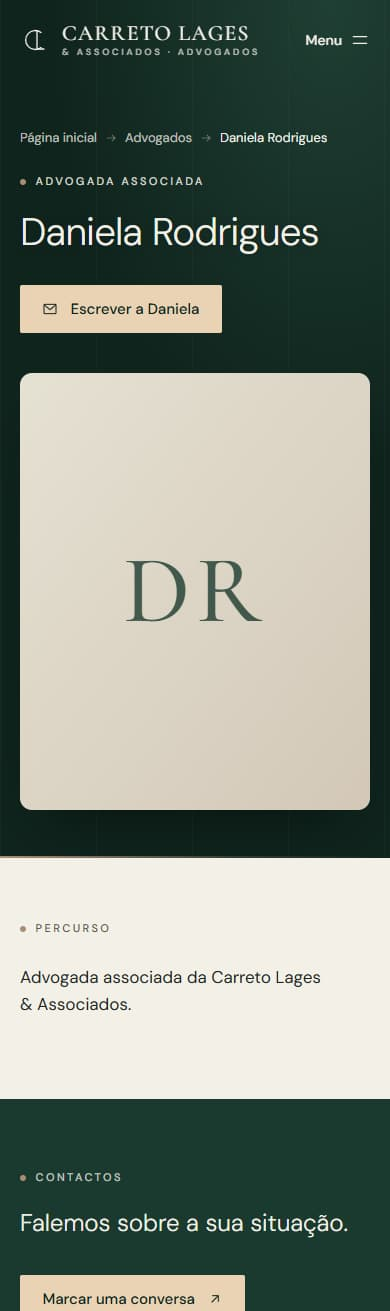
\includegraphics[width=0.235\textwidth]{screenshots/mobile/pt/advogados--daniela-rodrigues-1.jpg}\hspace{0.012\textwidth}
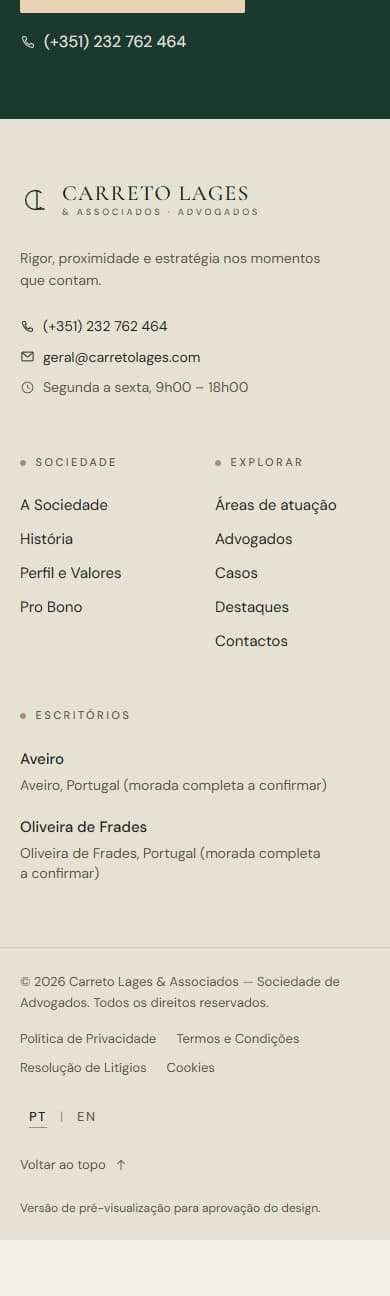
\includegraphics[width=0.235\textwidth]{screenshots/mobile/pt/advogados--daniela-rodrigues-2.jpg}\par\medskip
\bigskip
\needspace{8\baselineskip}
\subsection*{Diana Antão Seabra}
\addcontentsline{toc}{subsection}{Diana Antão Seabra (\texttt{/advogados/diana-antao-seabra})}
\noindent{\small\color{tintasuave}\texttt{/advogados/diana-antao-seabra}}\par\smallskip
\noindent{\footnotesize Computador (1440\,px)}\par\smallskip
\noindent 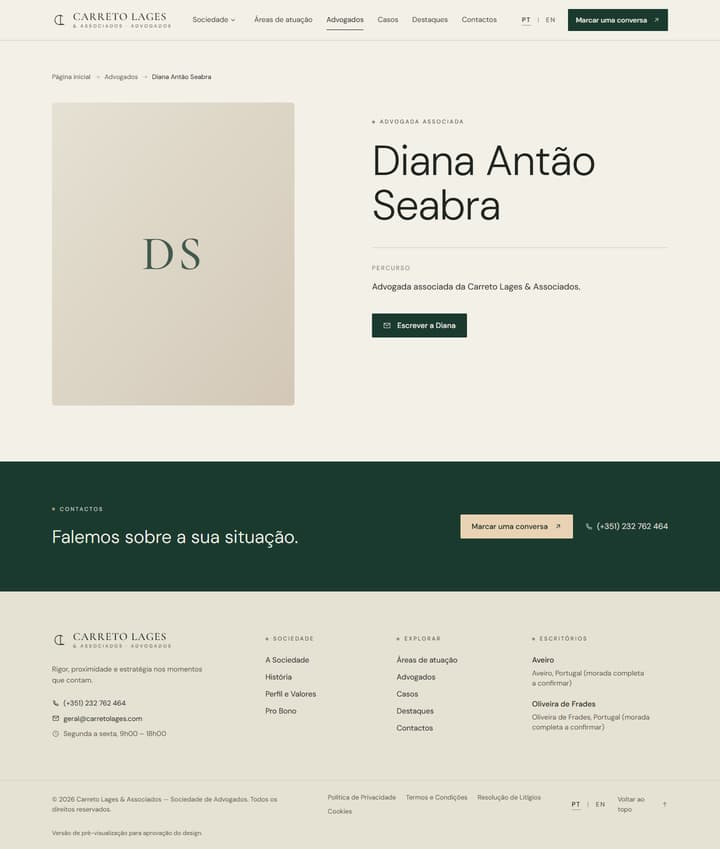
\includegraphics[width=0.485\textwidth]{screenshots/desktop/pt/advogados--diana-antao-seabra.jpg}\par\medskip
\noindent{\footnotesize Telemóvel (390\,px)}\par\smallskip
\noindent 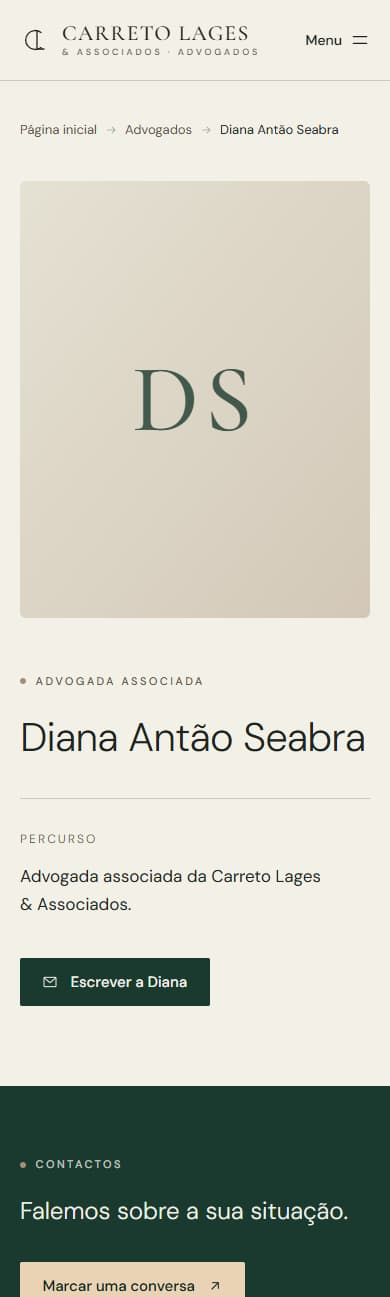
\includegraphics[width=0.235\textwidth]{screenshots/mobile/pt/advogados--diana-antao-seabra-1.jpg}\hspace{0.012\textwidth}
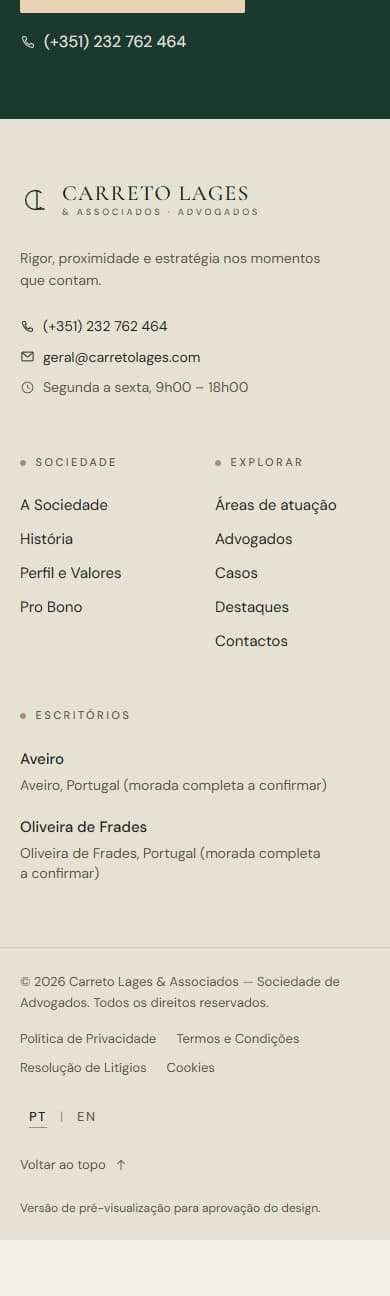
\includegraphics[width=0.235\textwidth]{screenshots/mobile/pt/advogados--diana-antao-seabra-2.jpg}\par\medskip
\bigskip
\needspace{8\baselineskip}
\subsection*{Francisco Lopes}
\addcontentsline{toc}{subsection}{Francisco Lopes (\texttt{/advogados/francisco-lopes})}
\noindent{\small\color{tintasuave}\texttt{/advogados/francisco-lopes}}\par\smallskip
\noindent{\footnotesize Computador (1440\,px)}\par\smallskip
\noindent 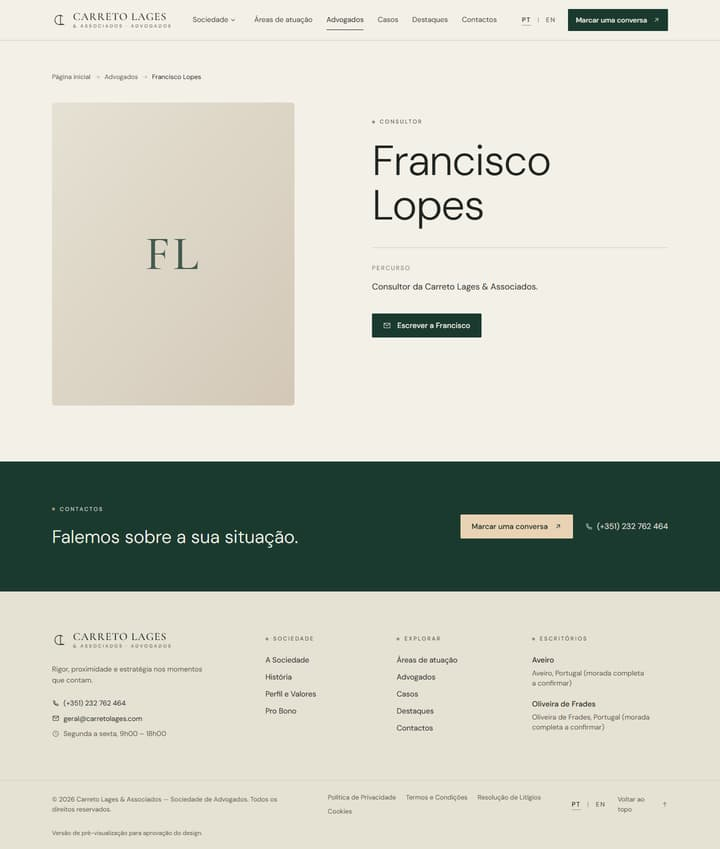
\includegraphics[width=0.485\textwidth]{screenshots/desktop/pt/advogados--francisco-lopes.jpg}\par\medskip
\noindent{\footnotesize Telemóvel (390\,px)}\par\smallskip
\noindent 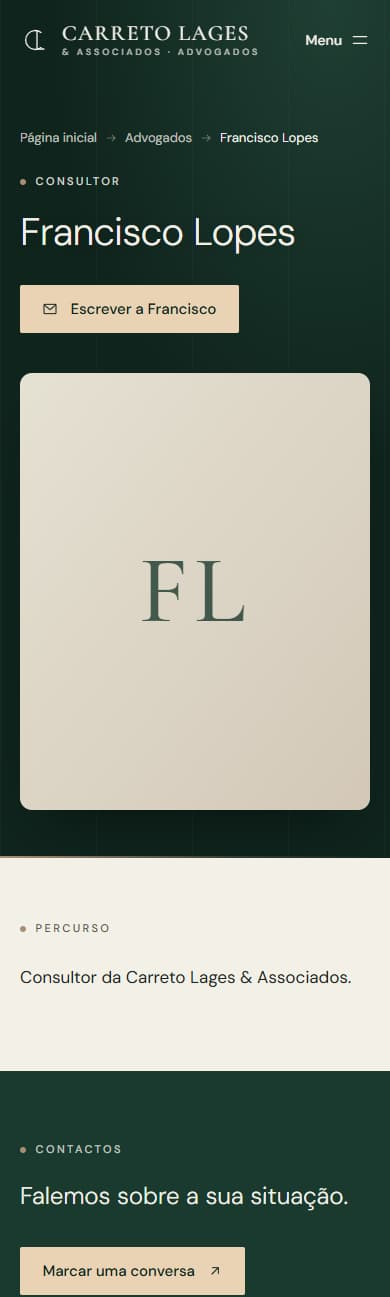
\includegraphics[width=0.235\textwidth]{screenshots/mobile/pt/advogados--francisco-lopes-1.jpg}\hspace{0.012\textwidth}
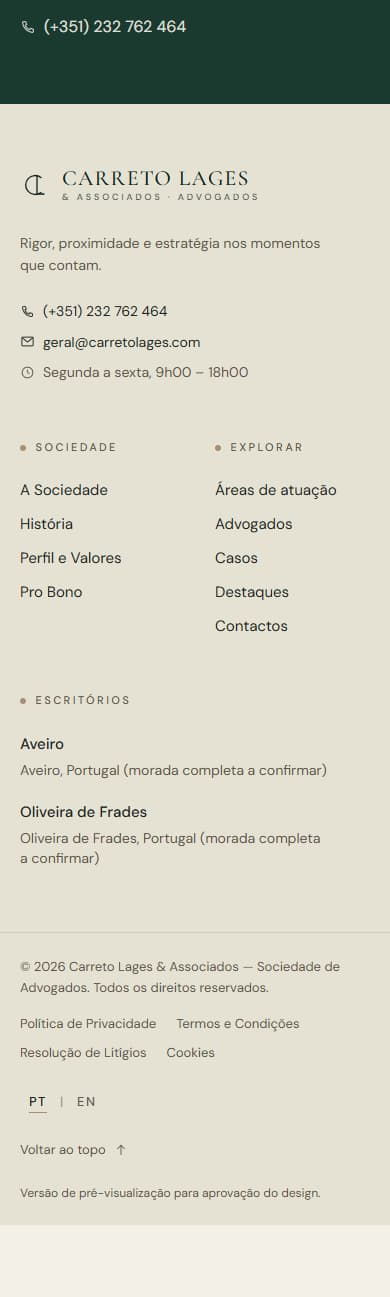
\includegraphics[width=0.235\textwidth]{screenshots/mobile/pt/advogados--francisco-lopes-2.jpg}\par\medskip
\bigskip
\needspace{8\baselineskip}
\subsection*{João Carlos Lages}
\addcontentsline{toc}{subsection}{João Carlos Lages (\texttt{/advogados/joao-carlos-lages})}
\noindent{\small\color{tintasuave}\texttt{/advogados/joao-carlos-lages}}\par\smallskip
\noindent{\footnotesize Computador (1440\,px)}\par\smallskip
\noindent 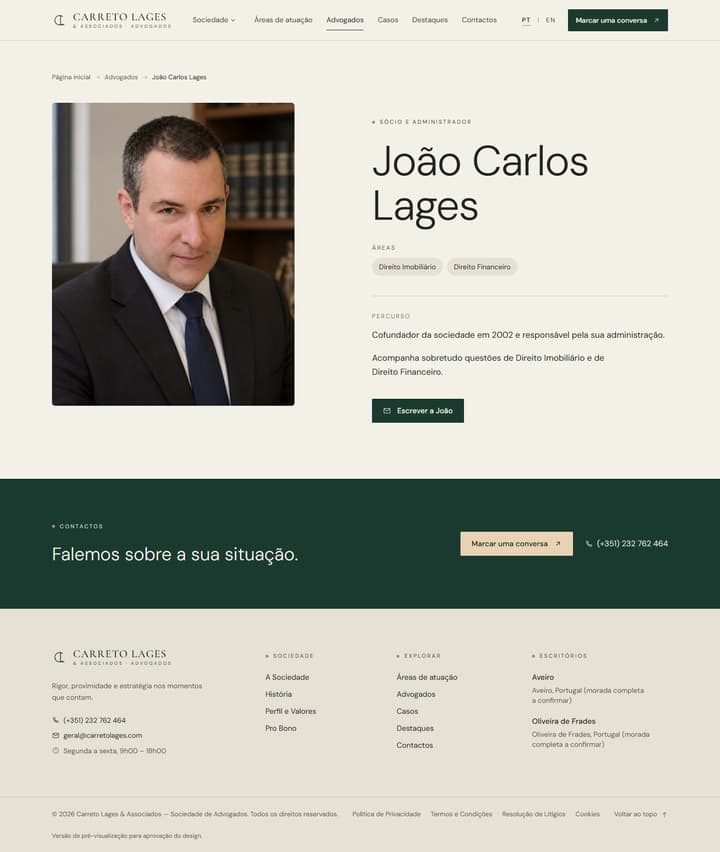
\includegraphics[width=0.485\textwidth]{screenshots/desktop/pt/advogados--joao-carlos-lages.jpg}\par\medskip
\noindent{\footnotesize Telemóvel (390\,px)}\par\smallskip
\noindent 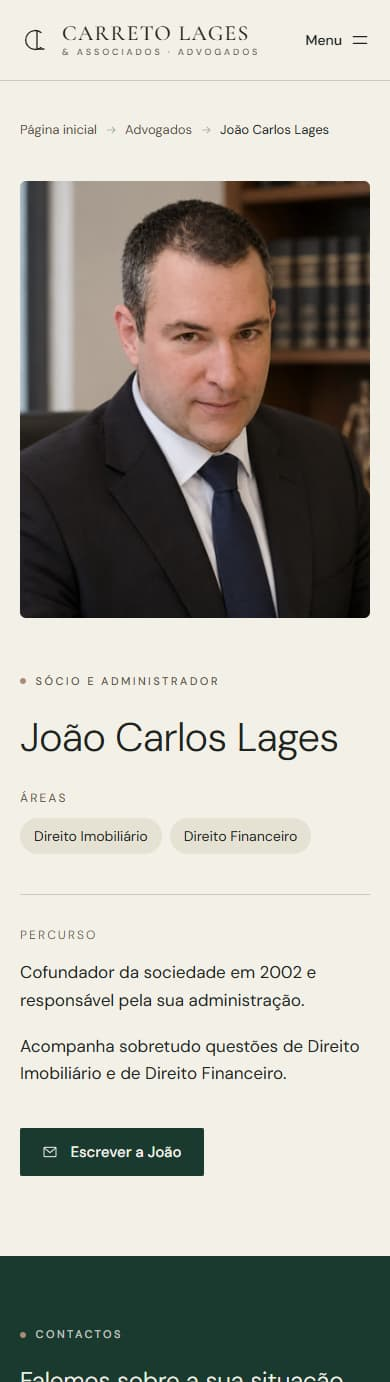
\includegraphics[width=0.235\textwidth]{screenshots/mobile/pt/advogados--joao-carlos-lages-1.jpg}\hspace{0.012\textwidth}
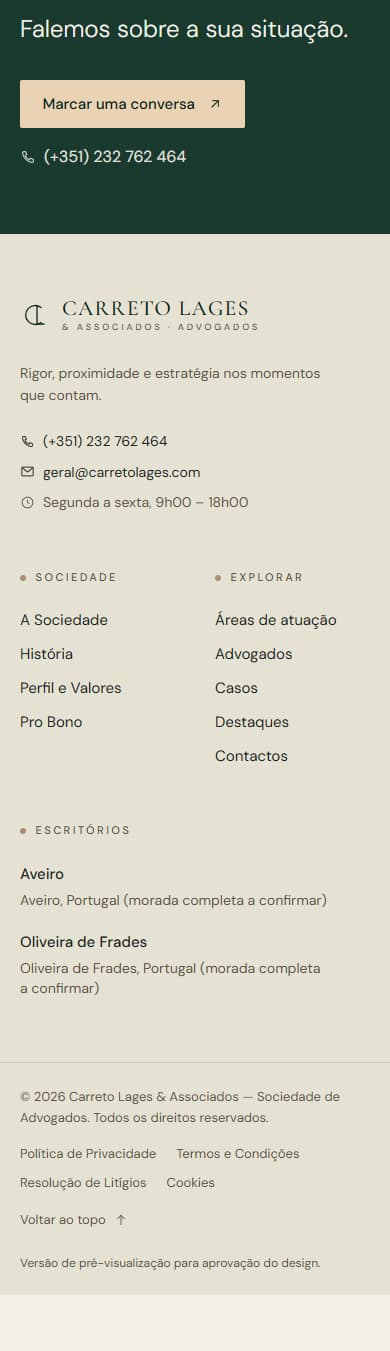
\includegraphics[width=0.235\textwidth]{screenshots/mobile/pt/advogados--joao-carlos-lages-2.jpg}\par\medskip
\bigskip
\needspace{8\baselineskip}
\subsection*{José Carreto Lages}
\addcontentsline{toc}{subsection}{José Carreto Lages (\texttt{/advogados/jose-carreto-lages})}
\noindent{\small\color{tintasuave}\texttt{/advogados/jose-carreto-lages}}\par\smallskip
\noindent{\footnotesize Computador (1440\,px)}\par\smallskip
\noindent 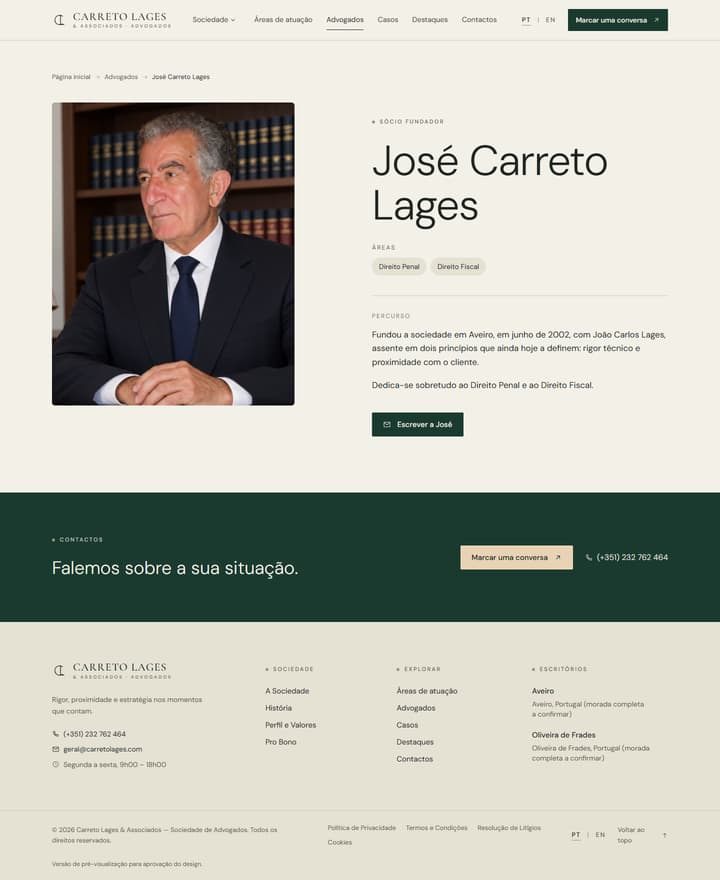
\includegraphics[width=0.485\textwidth]{screenshots/desktop/pt/advogados--jose-carreto-lages.jpg}\par\medskip
\noindent{\footnotesize Telemóvel (390\,px)}\par\smallskip
\noindent 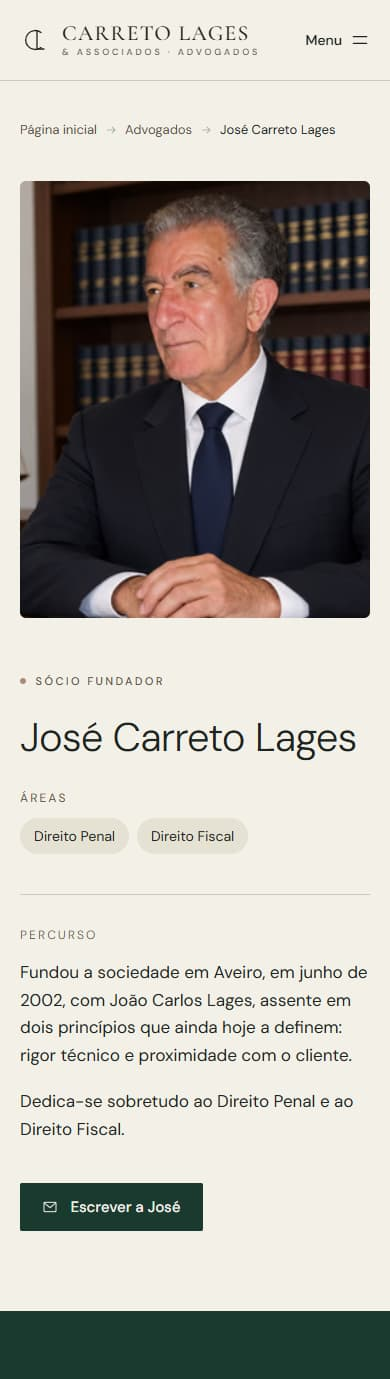
\includegraphics[width=0.235\textwidth]{screenshots/mobile/pt/advogados--jose-carreto-lages-1.jpg}\hspace{0.012\textwidth}
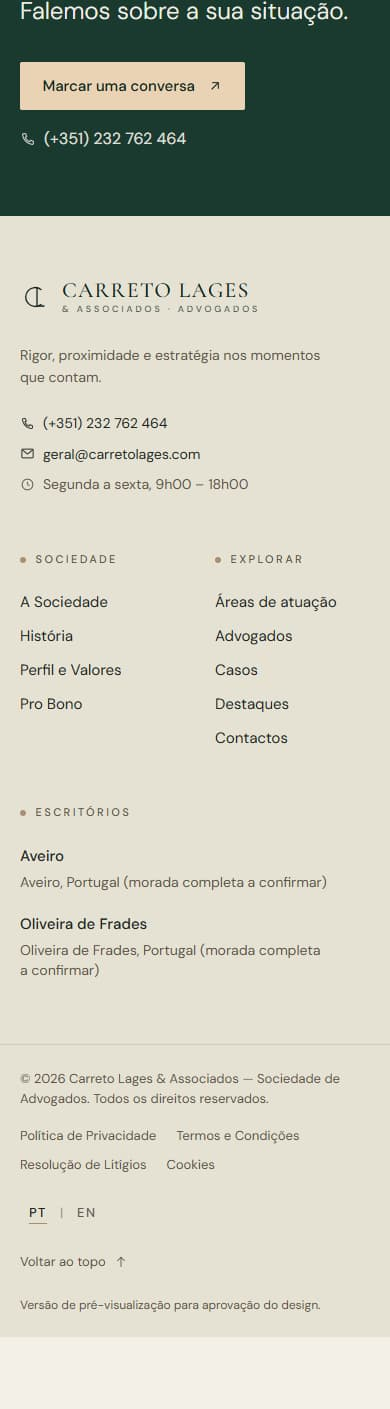
\includegraphics[width=0.235\textwidth]{screenshots/mobile/pt/advogados--jose-carreto-lages-2.jpg}\par\medskip
\bigskip
\needspace{8\baselineskip}
\subsection*{Sara Matos}
\addcontentsline{toc}{subsection}{Sara Matos (\texttt{/advogados/sara-matos})}
\noindent{\small\color{tintasuave}\texttt{/advogados/sara-matos}}\par\smallskip
\noindent{\footnotesize Computador (1440\,px)}\par\smallskip
\noindent 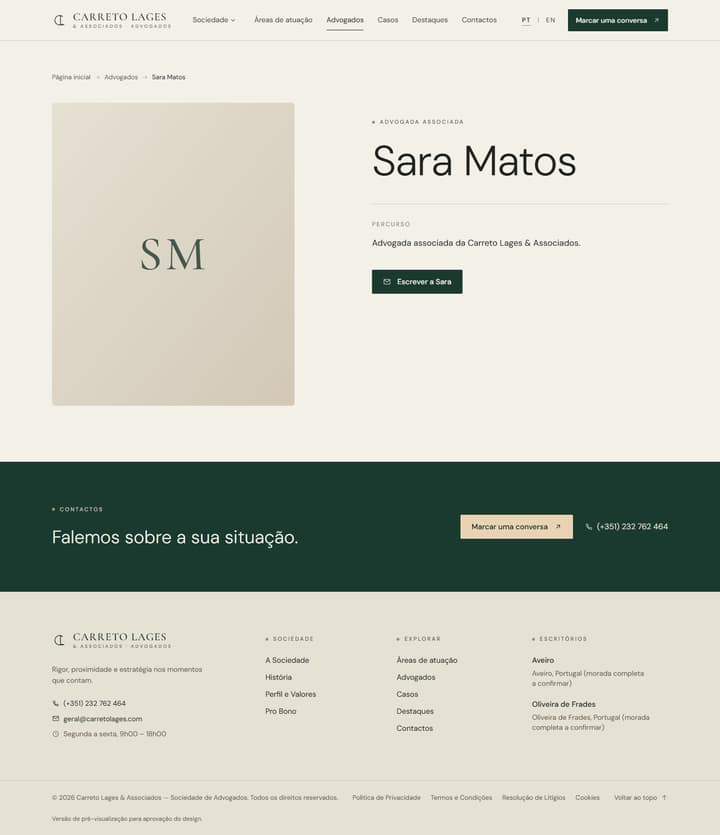
\includegraphics[width=0.485\textwidth]{screenshots/desktop/pt/advogados--sara-matos.jpg}\par\medskip
\noindent{\footnotesize Telemóvel (390\,px)}\par\smallskip
\noindent 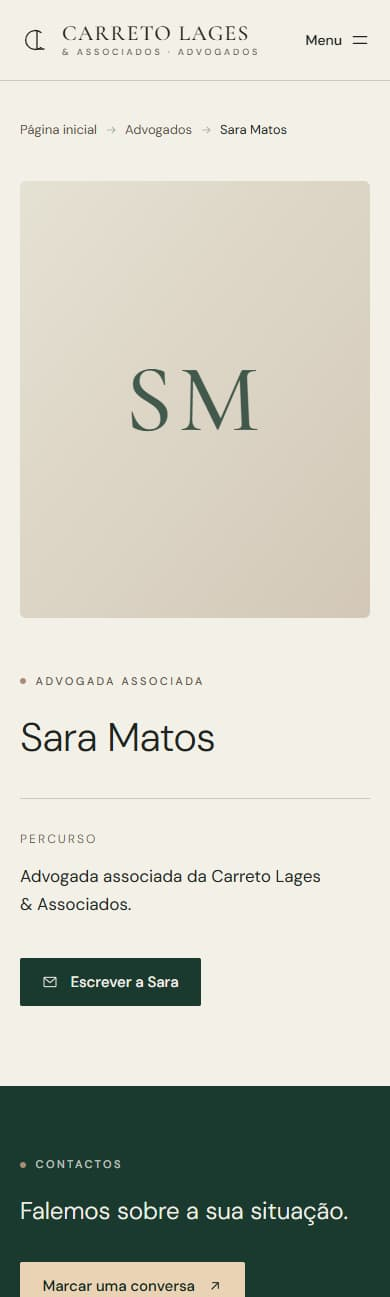
\includegraphics[width=0.235\textwidth]{screenshots/mobile/pt/advogados--sara-matos-1.jpg}\hspace{0.012\textwidth}
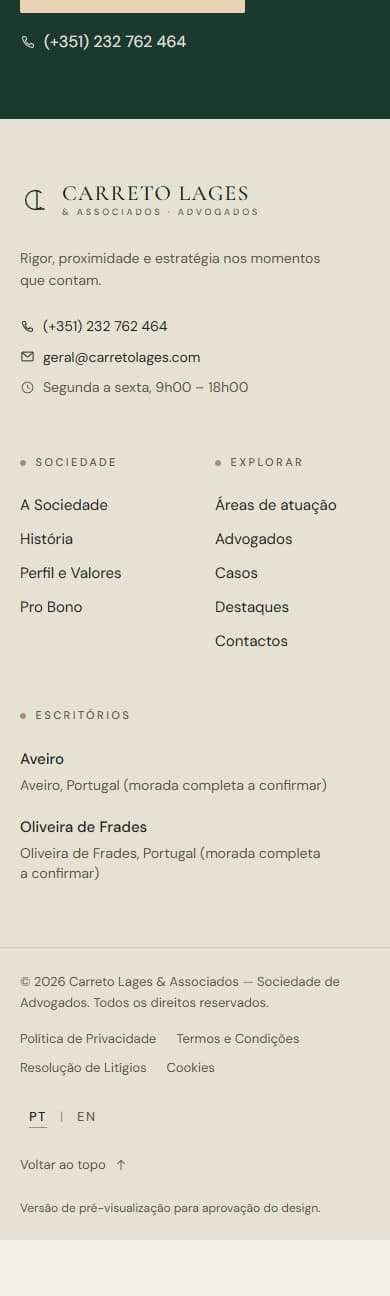
\includegraphics[width=0.235\textwidth]{screenshots/mobile/pt/advogados--sara-matos-2.jpg}\par\medskip
\bigskip
\needspace{8\baselineskip}
\subsection*{Experiência para o que vem a seguir.}
\addcontentsline{toc}{subsection}{Experiência para o que vem a seguir. (\texttt{/areas-de-atuacao})}
\noindent{\small\color{tintasuave}\texttt{/areas-de-atuacao}}\par\smallskip
\noindent{\footnotesize Computador (1440\,px)}\par\smallskip
\noindent 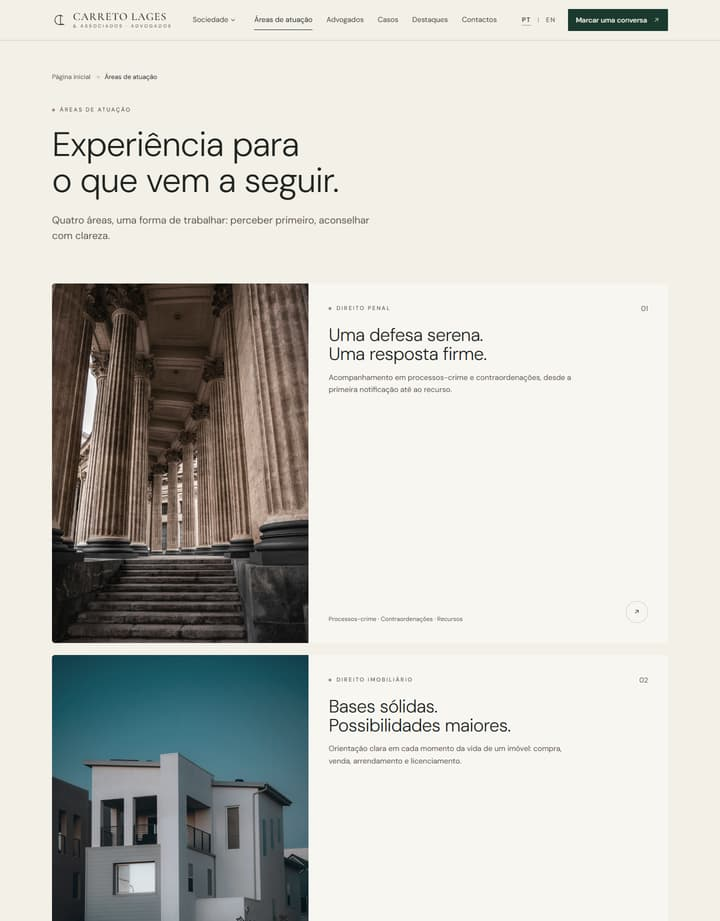
\includegraphics[width=0.485\textwidth]{screenshots/desktop/pt/areas-de-atuacao-1.jpg}\hspace{0.012\textwidth}
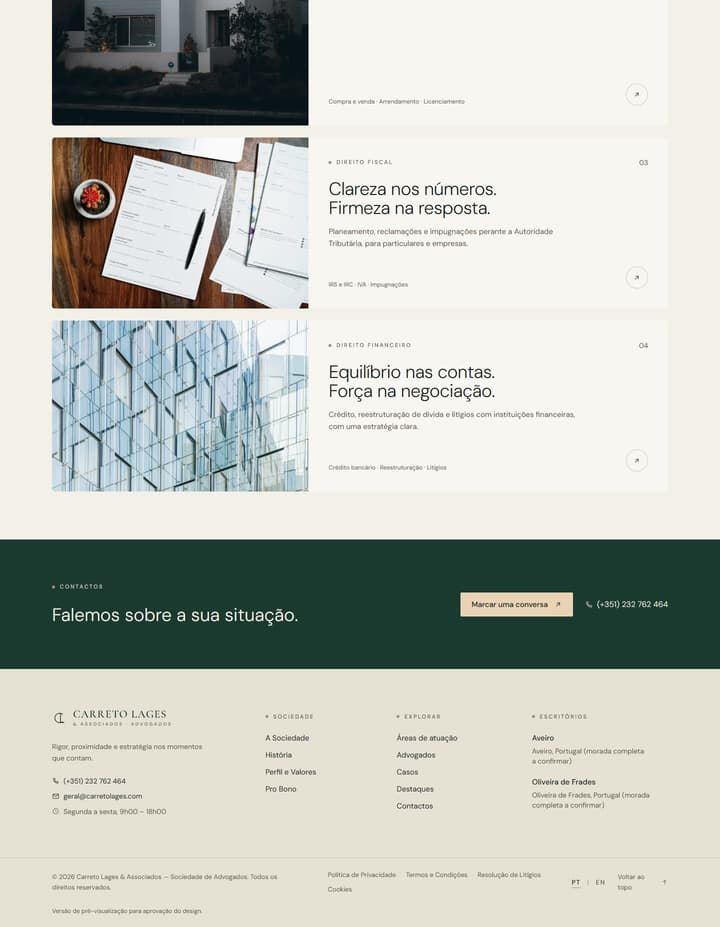
\includegraphics[width=0.485\textwidth]{screenshots/desktop/pt/areas-de-atuacao-2.jpg}\par\medskip
\noindent{\footnotesize Telemóvel (390\,px)}\par\smallskip
\noindent 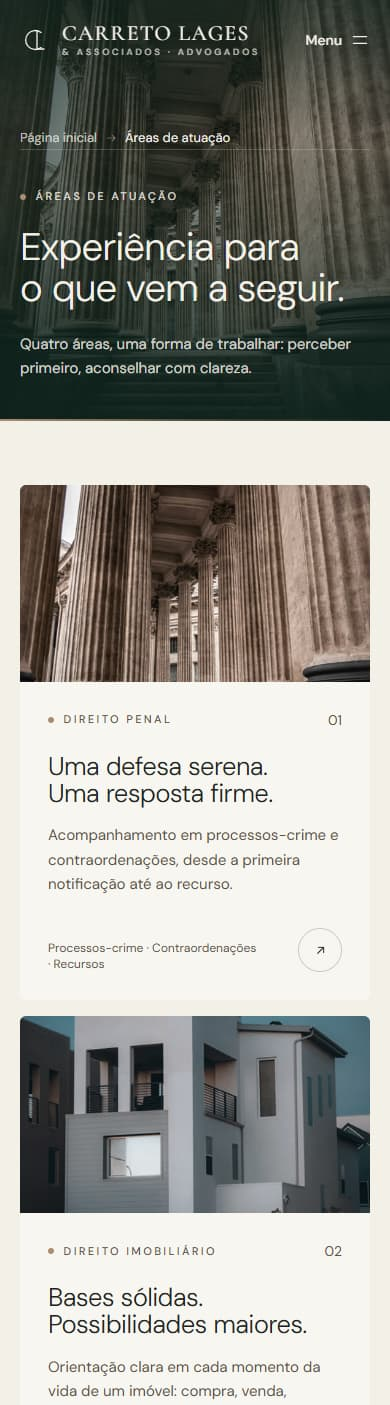
\includegraphics[width=0.235\textwidth]{screenshots/mobile/pt/areas-de-atuacao-1.jpg}\hspace{0.012\textwidth}
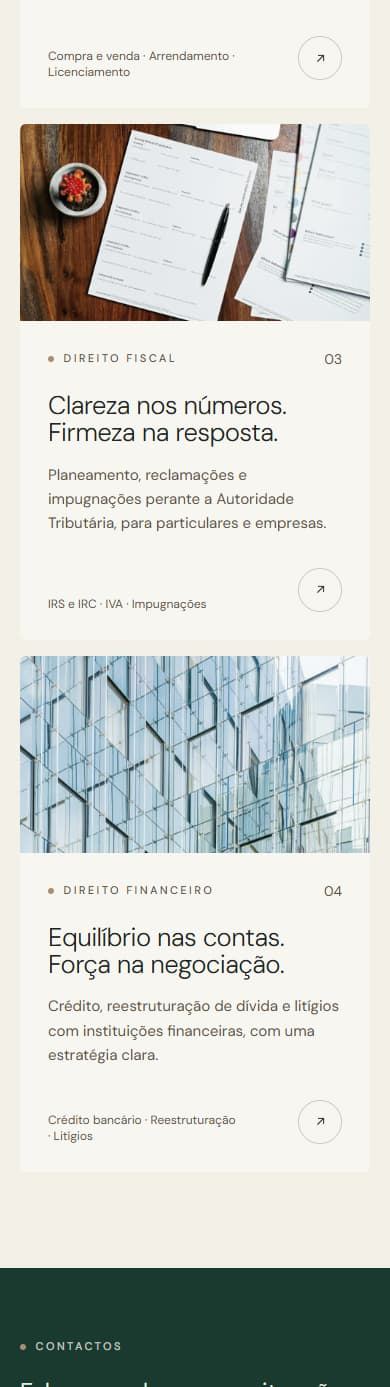
\includegraphics[width=0.235\textwidth]{screenshots/mobile/pt/areas-de-atuacao-2.jpg}\hspace{0.012\textwidth}
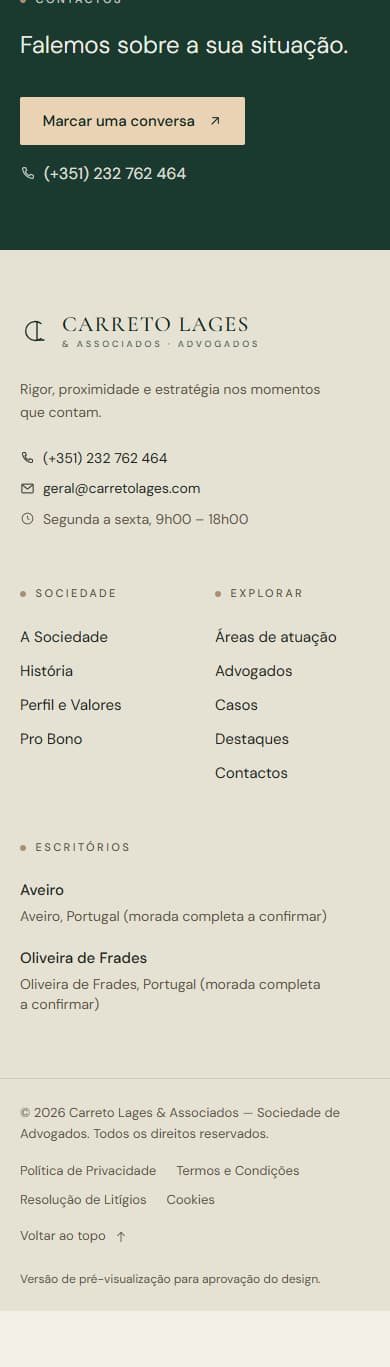
\includegraphics[width=0.235\textwidth]{screenshots/mobile/pt/areas-de-atuacao-3.jpg}\par\medskip
\bigskip
\needspace{8\baselineskip}
\subsection*{Equilíbrio nas contas. Força na negociação.}
\addcontentsline{toc}{subsection}{Equilíbrio nas contas. Força na negociação. (\texttt{/areas-de-atuacao/direito-financeiro})}
\noindent{\small\color{tintasuave}\texttt{/areas-de-atuacao/direito-financeiro}}\par\smallskip
\noindent{\footnotesize Computador (1440\,px)}\par\smallskip
\noindent 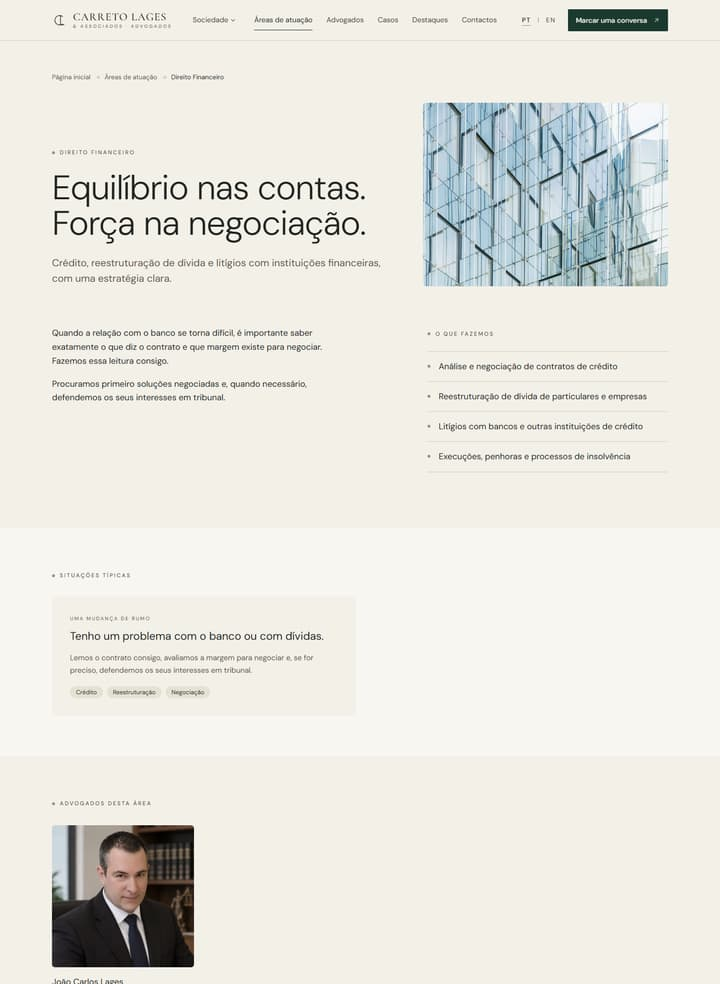
\includegraphics[width=0.485\textwidth]{screenshots/desktop/pt/areas-de-atuacao--direito-financeiro-1.jpg}\hspace{0.012\textwidth}
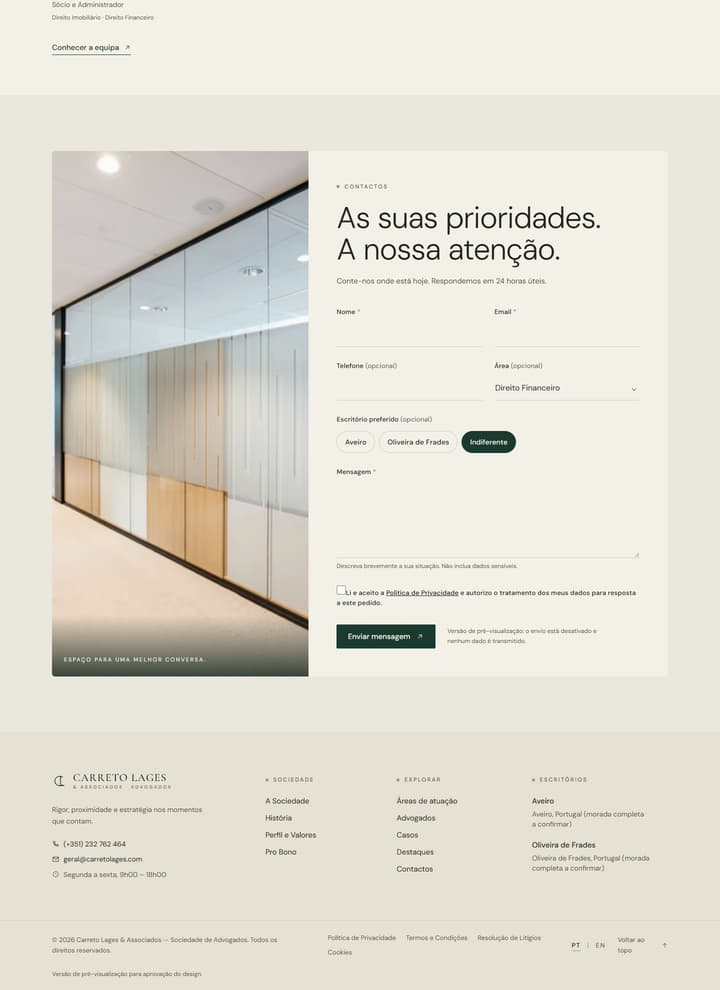
\includegraphics[width=0.485\textwidth]{screenshots/desktop/pt/areas-de-atuacao--direito-financeiro-2.jpg}\par\medskip
\noindent{\footnotesize Telemóvel (390\,px)}\par\smallskip
\noindent 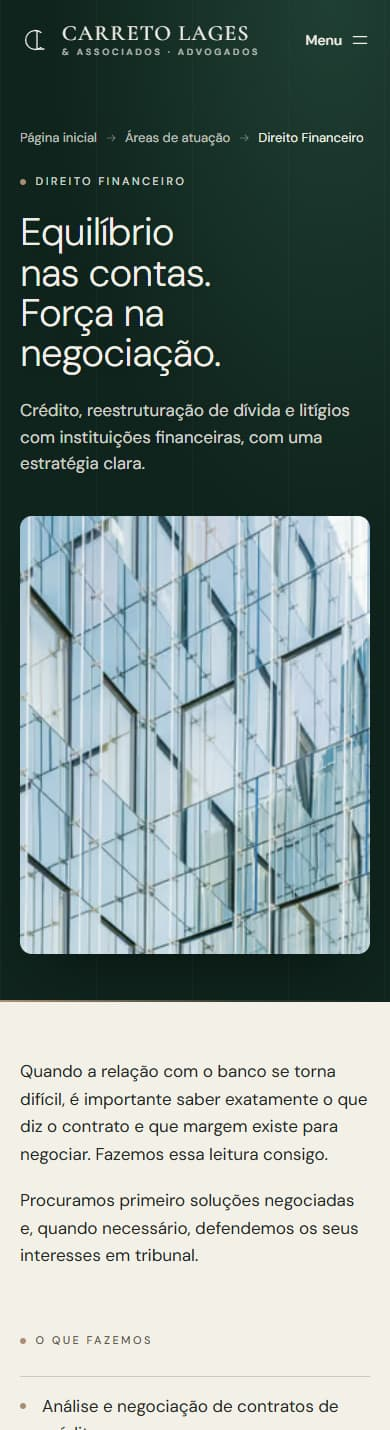
\includegraphics[width=0.235\textwidth]{screenshots/mobile/pt/areas-de-atuacao--direito-financeiro-1.jpg}\hspace{0.012\textwidth}
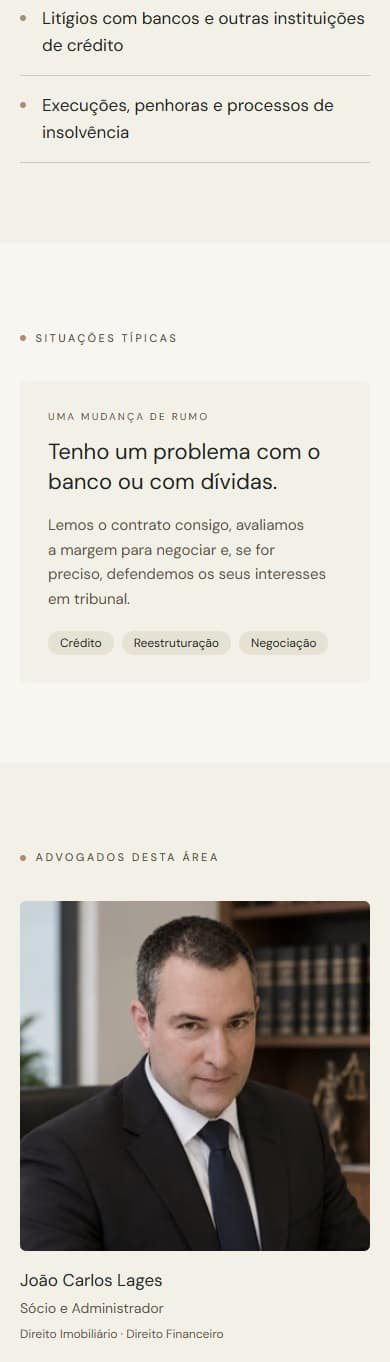
\includegraphics[width=0.235\textwidth]{screenshots/mobile/pt/areas-de-atuacao--direito-financeiro-2.jpg}\hspace{0.012\textwidth}
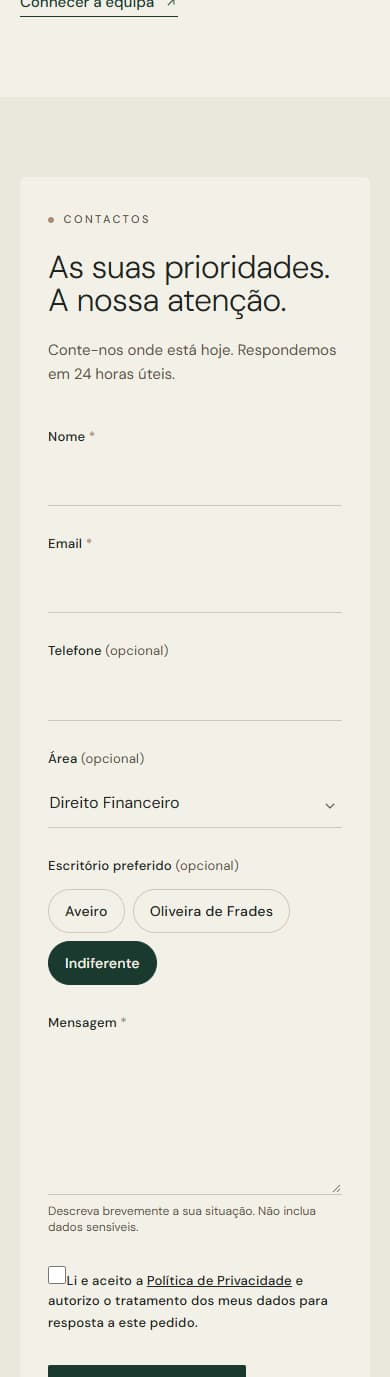
\includegraphics[width=0.235\textwidth]{screenshots/mobile/pt/areas-de-atuacao--direito-financeiro-3.jpg}\hspace{0.012\textwidth}
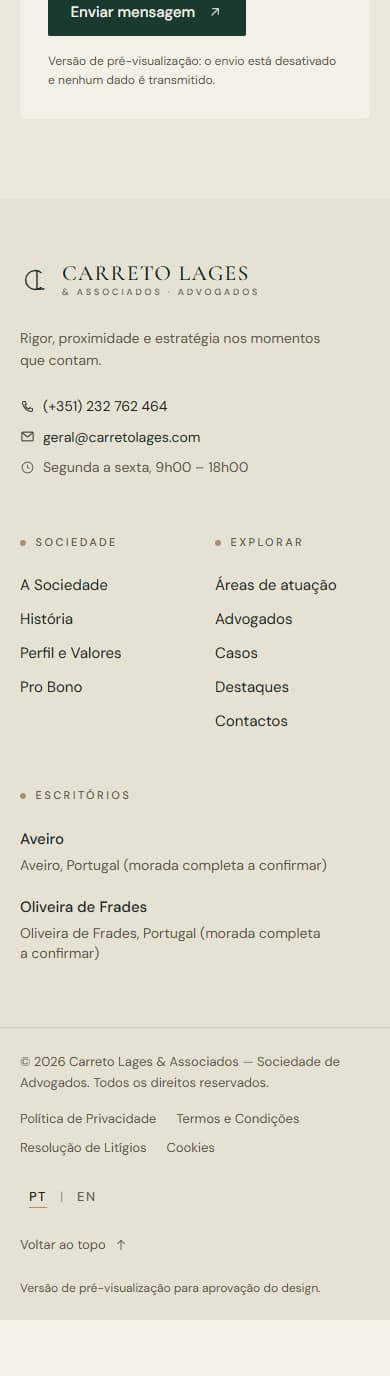
\includegraphics[width=0.235\textwidth]{screenshots/mobile/pt/areas-de-atuacao--direito-financeiro-4.jpg}\par\medskip
\bigskip
\needspace{8\baselineskip}
\subsection*{Clareza nos números. Firmeza na resposta.}
\addcontentsline{toc}{subsection}{Clareza nos números. Firmeza na resposta. (\texttt{/areas-de-atuacao/direito-fiscal})}
\noindent{\small\color{tintasuave}\texttt{/areas-de-atuacao/direito-fiscal}}\par\smallskip
\noindent{\footnotesize Computador (1440\,px)}\par\smallskip
\noindent 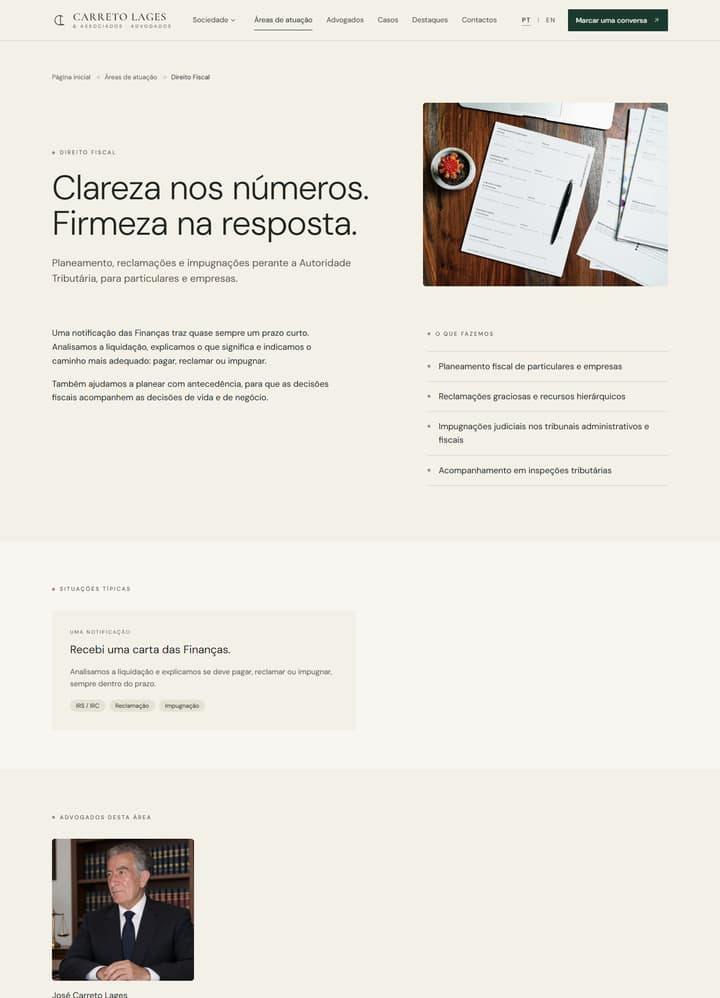
\includegraphics[width=0.485\textwidth]{screenshots/desktop/pt/areas-de-atuacao--direito-fiscal-1.jpg}\hspace{0.012\textwidth}
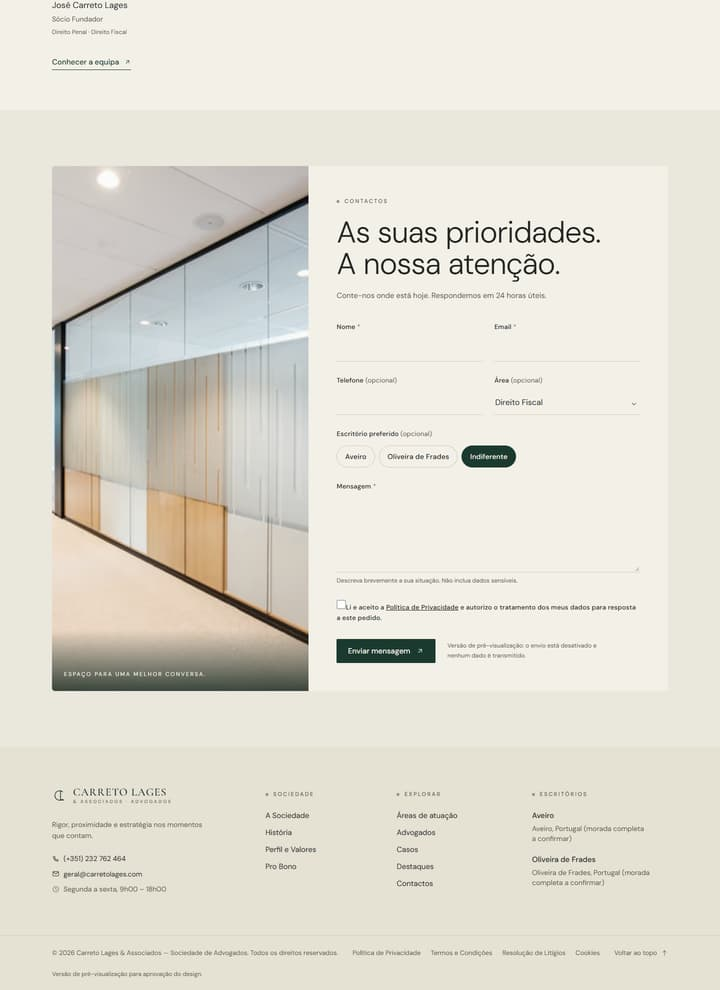
\includegraphics[width=0.485\textwidth]{screenshots/desktop/pt/areas-de-atuacao--direito-fiscal-2.jpg}\par\medskip
\noindent{\footnotesize Telemóvel (390\,px)}\par\smallskip
\noindent 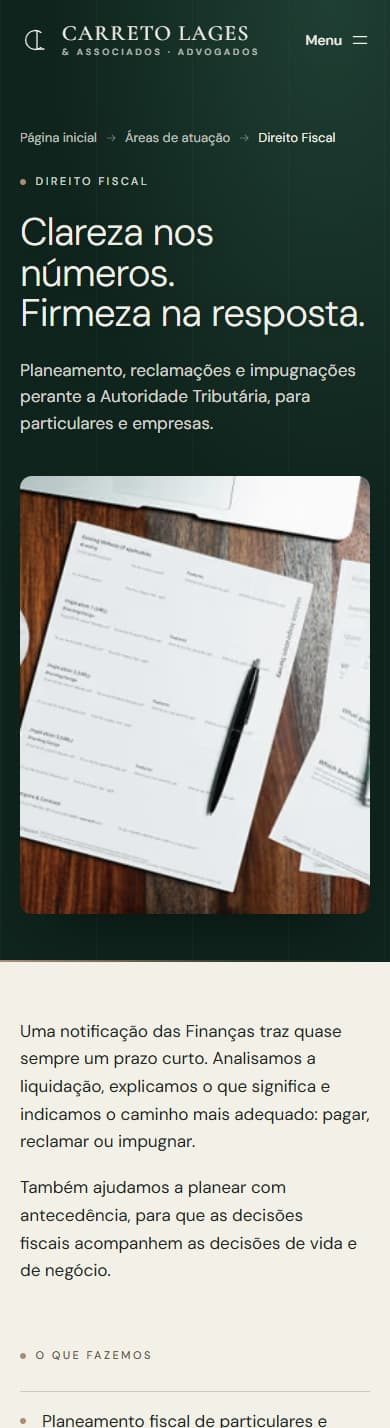
\includegraphics[width=0.235\textwidth]{screenshots/mobile/pt/areas-de-atuacao--direito-fiscal-1.jpg}\hspace{0.012\textwidth}
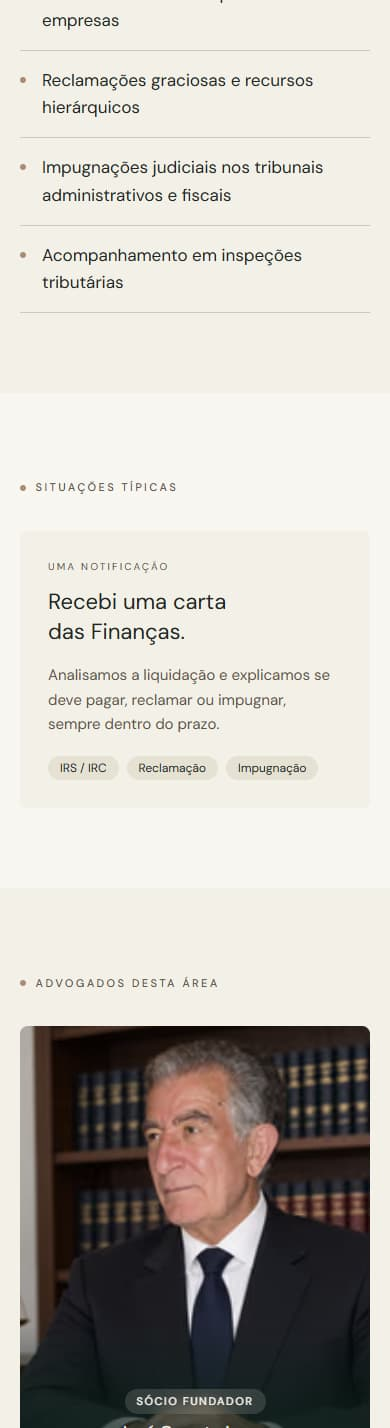
\includegraphics[width=0.235\textwidth]{screenshots/mobile/pt/areas-de-atuacao--direito-fiscal-2.jpg}\hspace{0.012\textwidth}
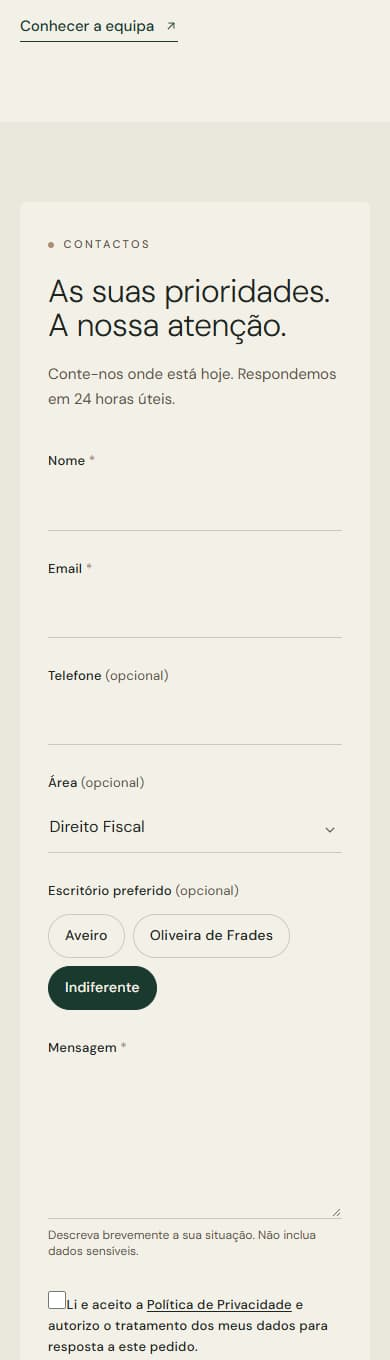
\includegraphics[width=0.235\textwidth]{screenshots/mobile/pt/areas-de-atuacao--direito-fiscal-3.jpg}\hspace{0.012\textwidth}
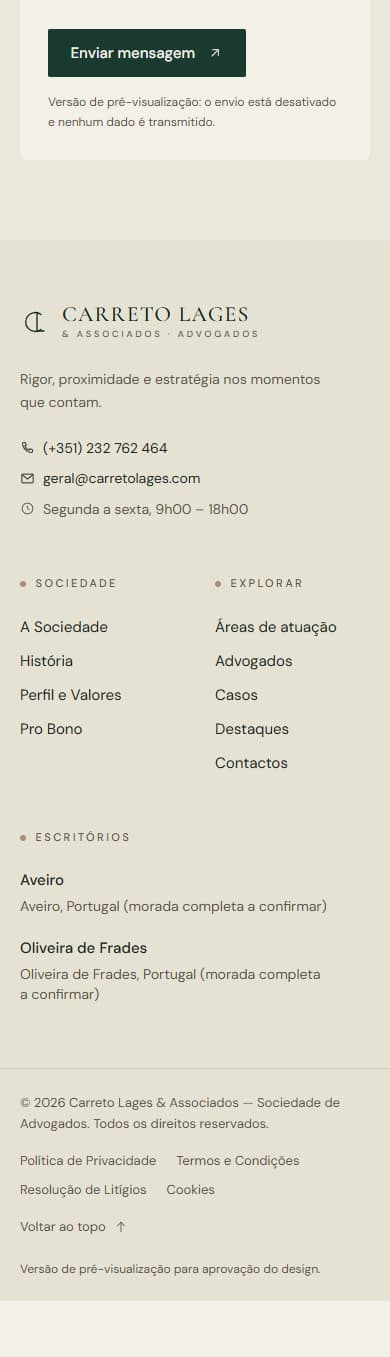
\includegraphics[width=0.235\textwidth]{screenshots/mobile/pt/areas-de-atuacao--direito-fiscal-4.jpg}\par\medskip
\bigskip
\needspace{8\baselineskip}
\subsection*{Bases sólidas. Possibilidades maiores.}
\addcontentsline{toc}{subsection}{Bases sólidas. Possibilidades maiores. (\texttt{/areas-de-atuacao/direito-imobiliario})}
\noindent{\small\color{tintasuave}\texttt{/areas-de-atuacao/direito-imobiliario}}\par\smallskip
\noindent{\footnotesize Computador (1440\,px)}\par\smallskip
\noindent 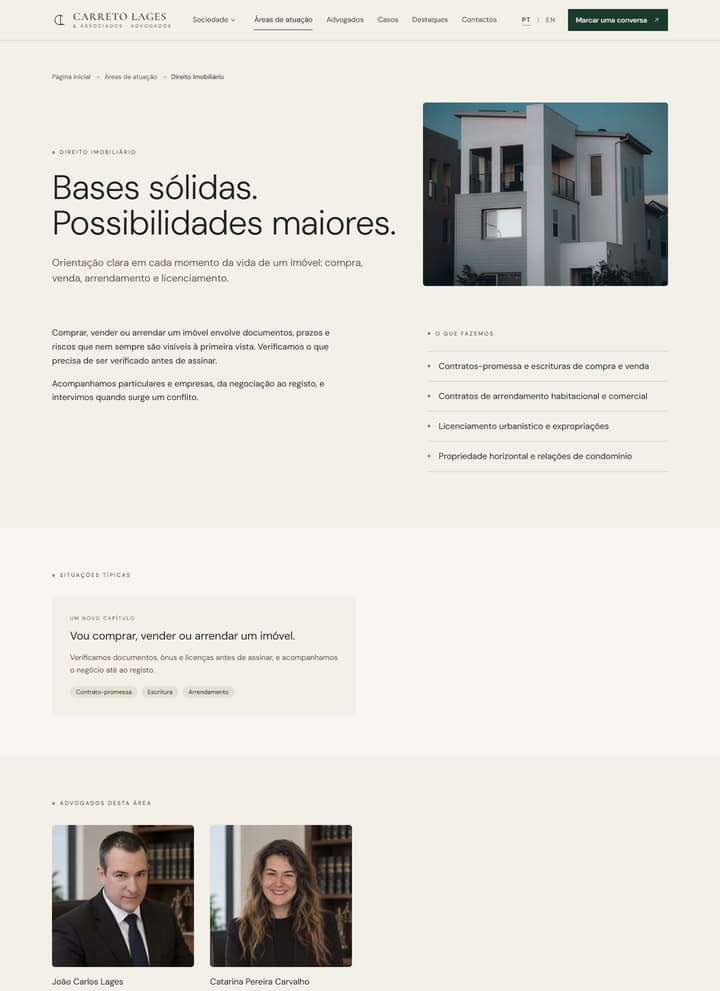
\includegraphics[width=0.485\textwidth]{screenshots/desktop/pt/areas-de-atuacao--direito-imobiliario-1.jpg}\hspace{0.012\textwidth}
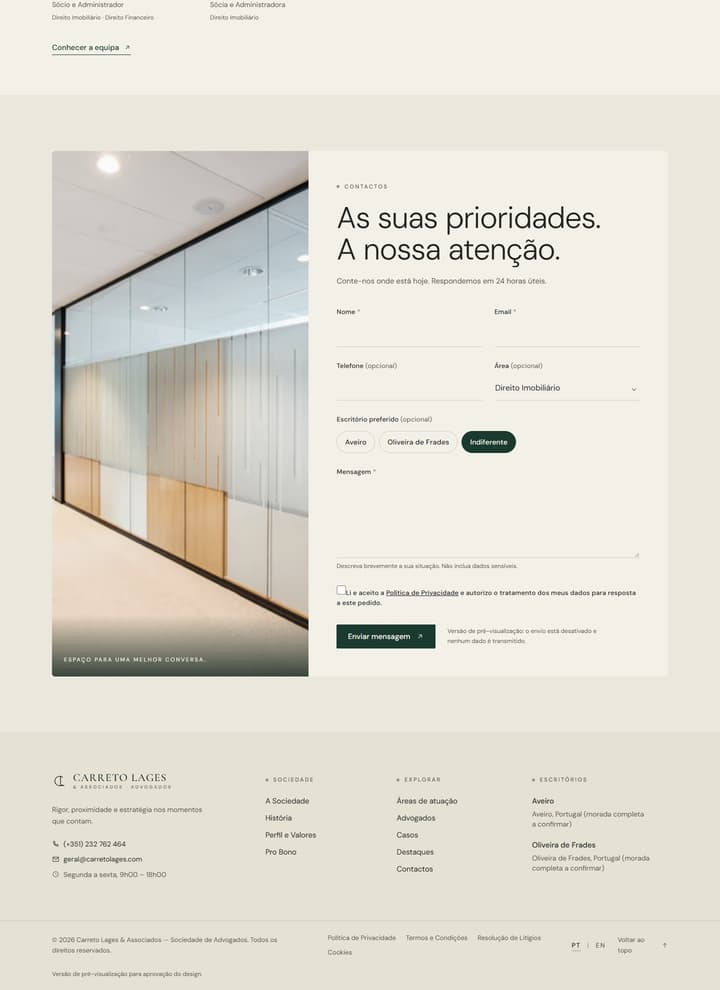
\includegraphics[width=0.485\textwidth]{screenshots/desktop/pt/areas-de-atuacao--direito-imobiliario-2.jpg}\par\medskip
\noindent{\footnotesize Telemóvel (390\,px)}\par\smallskip
\noindent 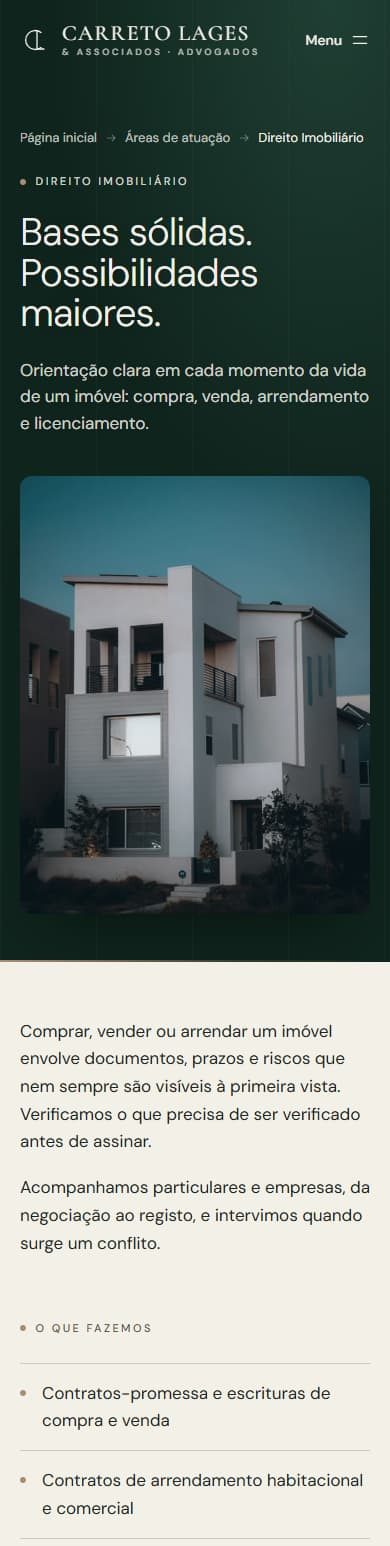
\includegraphics[width=0.235\textwidth]{screenshots/mobile/pt/areas-de-atuacao--direito-imobiliario-1.jpg}\hspace{0.012\textwidth}
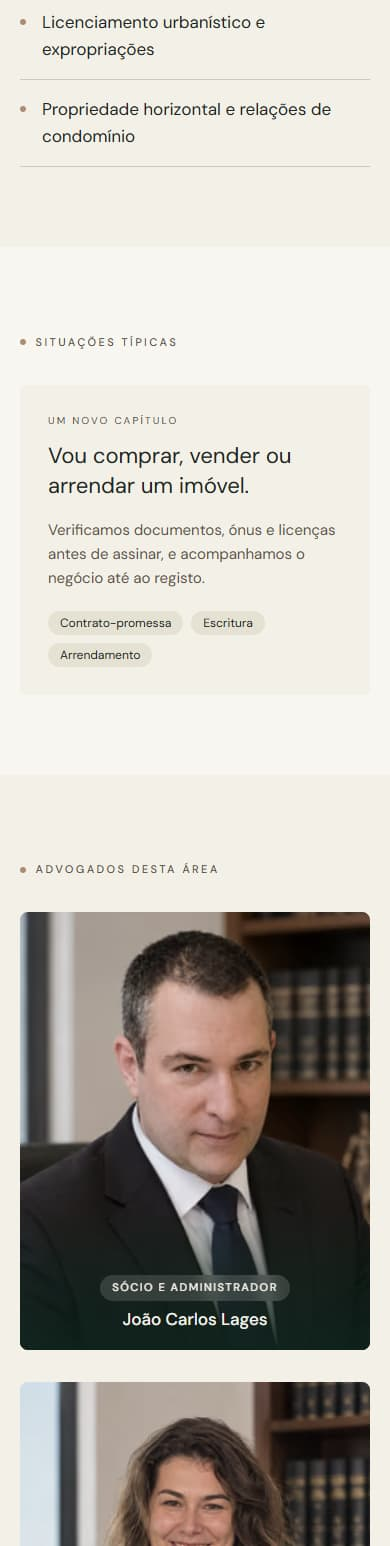
\includegraphics[width=0.235\textwidth]{screenshots/mobile/pt/areas-de-atuacao--direito-imobiliario-2.jpg}\hspace{0.012\textwidth}
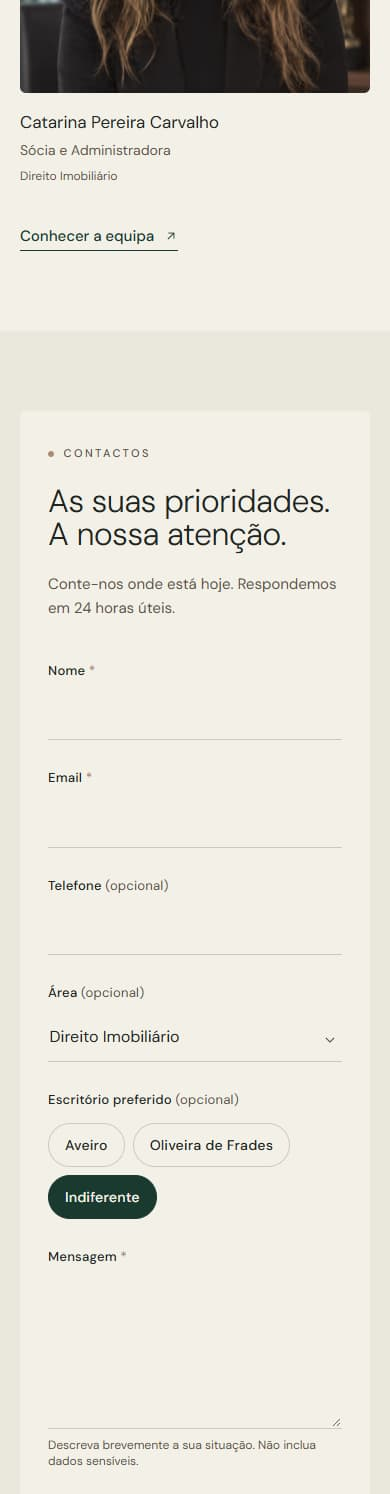
\includegraphics[width=0.235\textwidth]{screenshots/mobile/pt/areas-de-atuacao--direito-imobiliario-3.jpg}\hspace{0.012\textwidth}
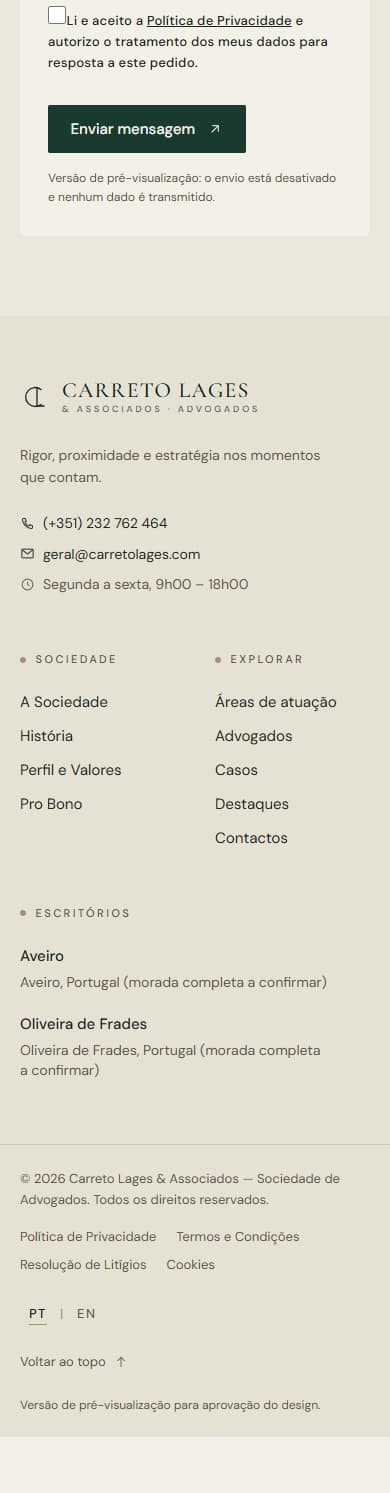
\includegraphics[width=0.235\textwidth]{screenshots/mobile/pt/areas-de-atuacao--direito-imobiliario-4.jpg}\par\medskip
\bigskip
\needspace{8\baselineskip}
\subsection*{Uma defesa serena. Uma resposta firme.}
\addcontentsline{toc}{subsection}{Uma defesa serena. Uma resposta firme. (\texttt{/areas-de-atuacao/direito-penal})}
\noindent{\small\color{tintasuave}\texttt{/areas-de-atuacao/direito-penal}}\par\smallskip
\noindent{\footnotesize Computador (1440\,px)}\par\smallskip
\noindent 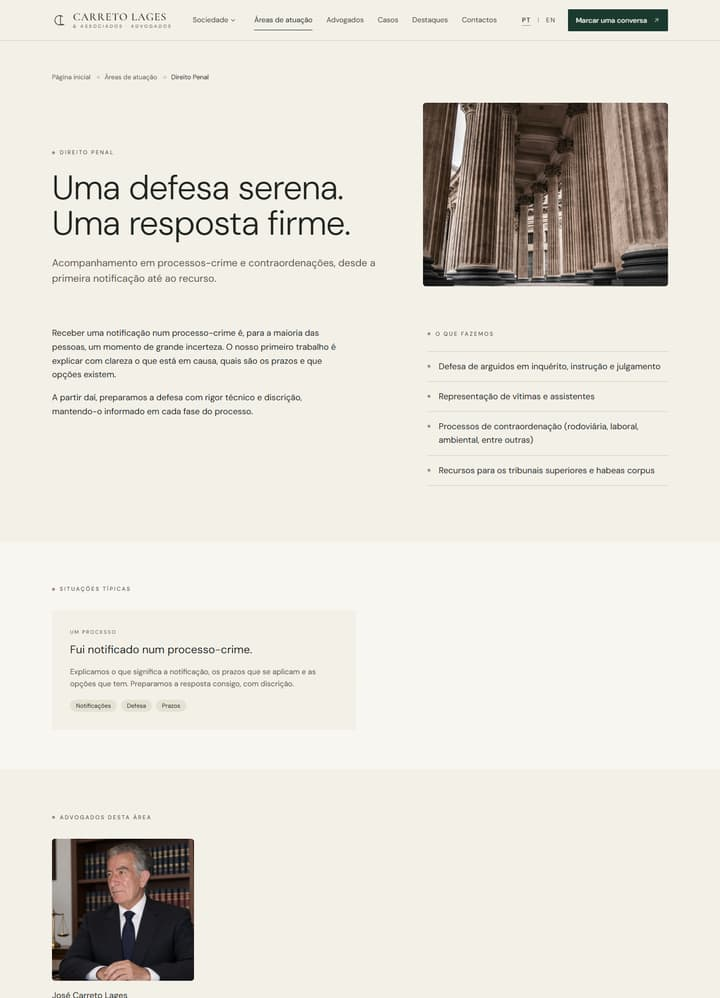
\includegraphics[width=0.485\textwidth]{screenshots/desktop/pt/areas-de-atuacao--direito-penal-1.jpg}\hspace{0.012\textwidth}
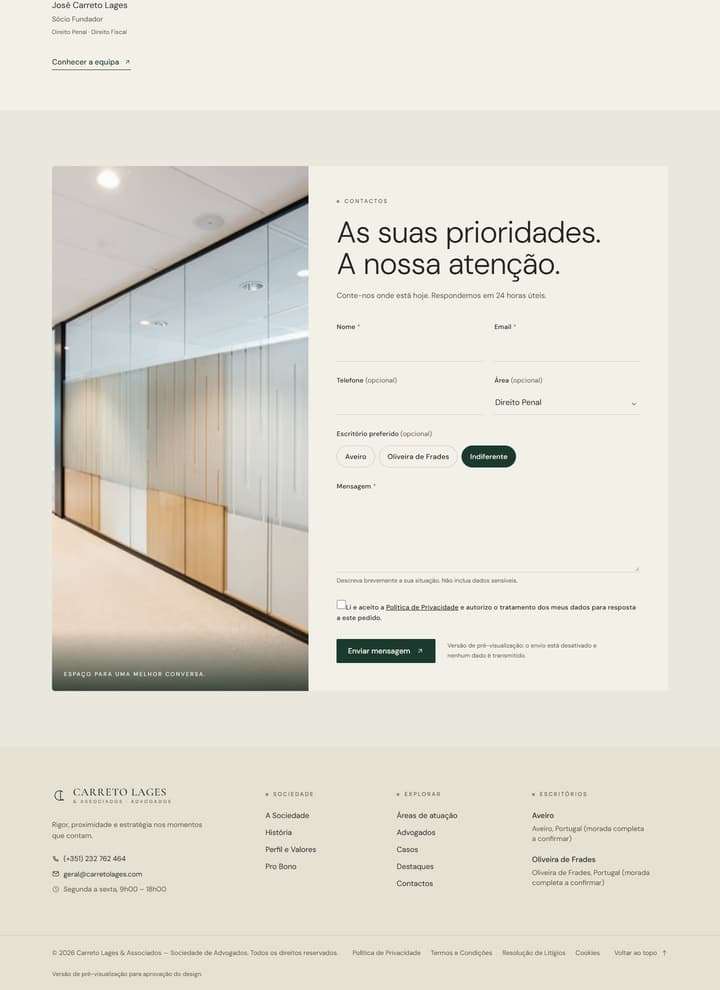
\includegraphics[width=0.485\textwidth]{screenshots/desktop/pt/areas-de-atuacao--direito-penal-2.jpg}\par\medskip
\noindent{\footnotesize Telemóvel (390\,px)}\par\smallskip
\noindent 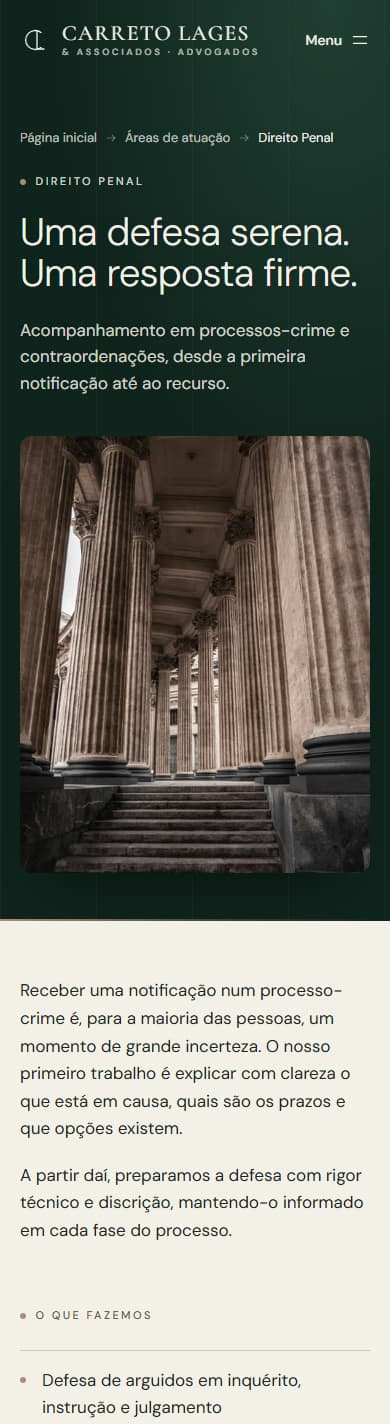
\includegraphics[width=0.235\textwidth]{screenshots/mobile/pt/areas-de-atuacao--direito-penal-1.jpg}\hspace{0.012\textwidth}
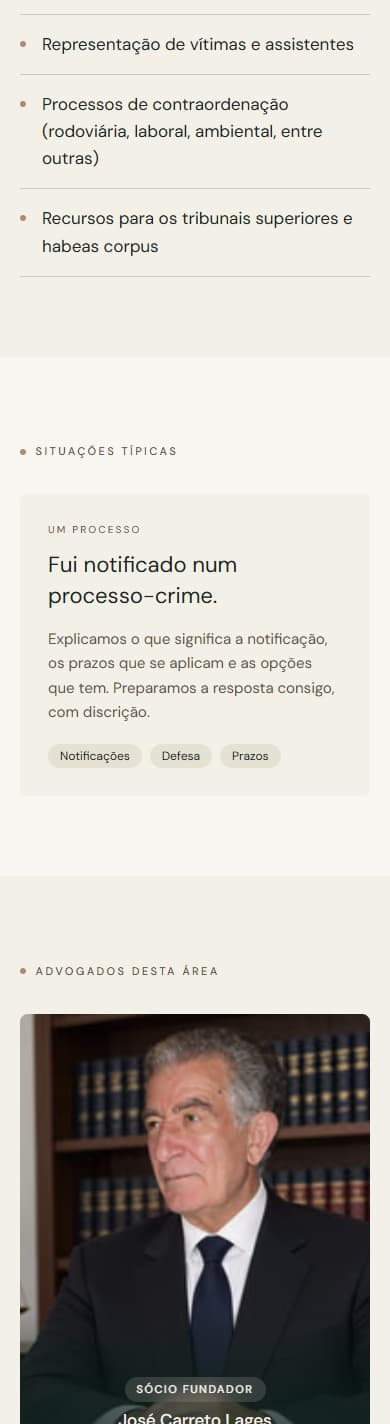
\includegraphics[width=0.235\textwidth]{screenshots/mobile/pt/areas-de-atuacao--direito-penal-2.jpg}\hspace{0.012\textwidth}
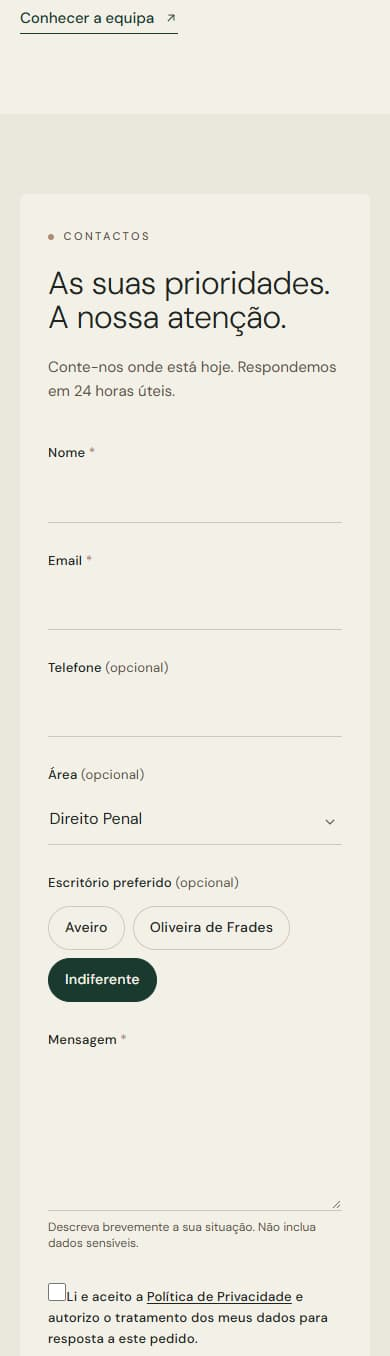
\includegraphics[width=0.235\textwidth]{screenshots/mobile/pt/areas-de-atuacao--direito-penal-3.jpg}\hspace{0.012\textwidth}
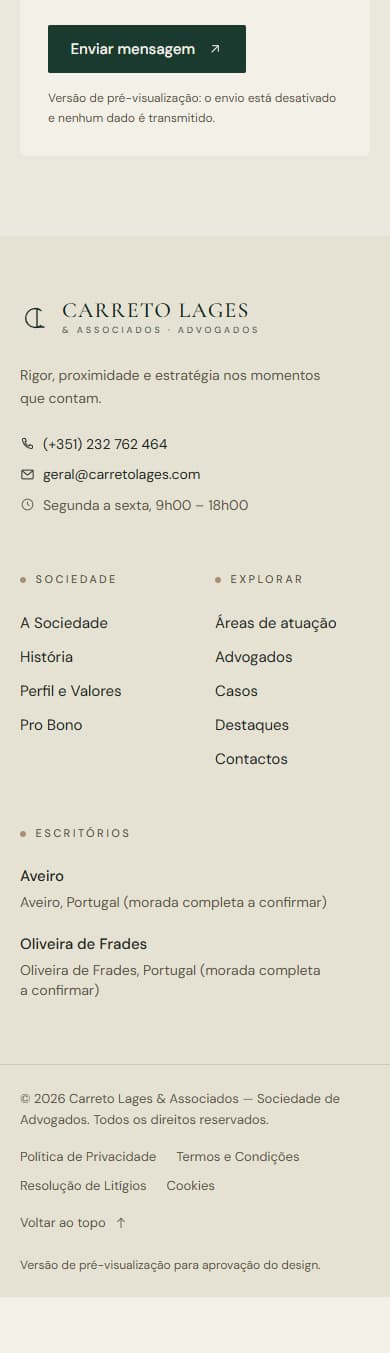
\includegraphics[width=0.235\textwidth]{screenshots/mobile/pt/areas-de-atuacao--direito-penal-4.jpg}\par\medskip
\bigskip
\needspace{8\baselineskip}
\subsection*{O nosso trabalho, em casos concretos.}
\addcontentsline{toc}{subsection}{O nosso trabalho, em casos concretos. (\texttt{/casos})}
\noindent{\small\color{tintasuave}\texttt{/casos}}\par\smallskip
\noindent{\footnotesize Computador (1440\,px)}\par\smallskip
\noindent 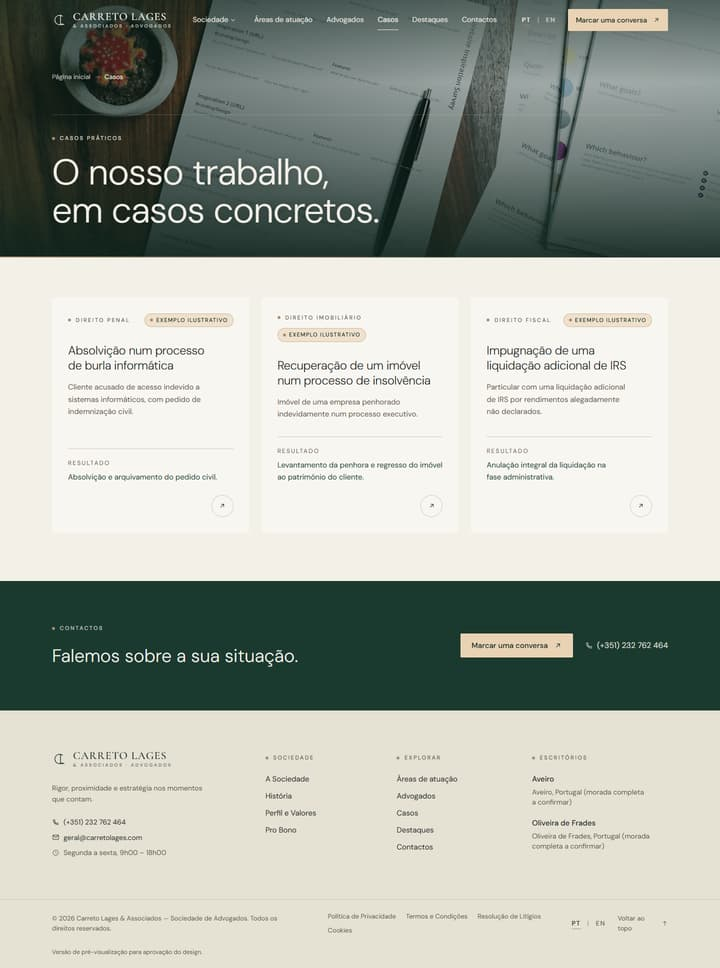
\includegraphics[width=0.485\textwidth]{screenshots/desktop/pt/casos.jpg}\par\medskip
\noindent{\footnotesize Telemóvel (390\,px)}\par\smallskip
\noindent 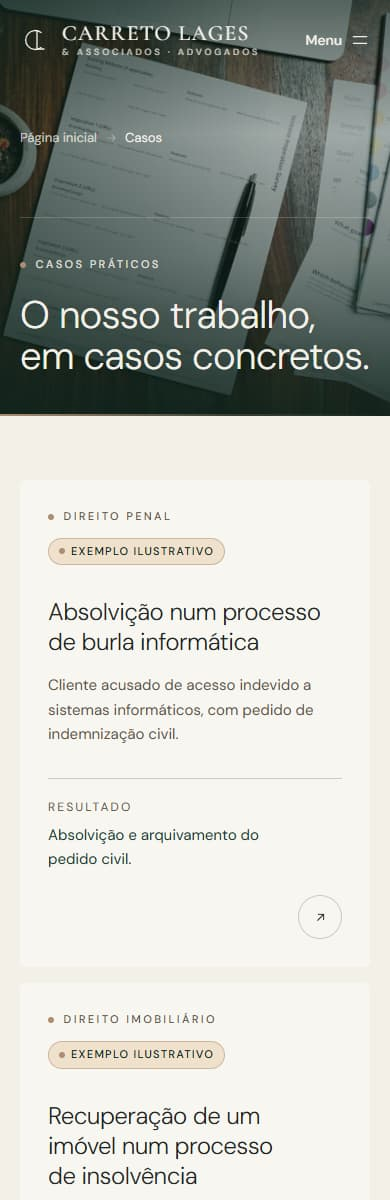
\includegraphics[width=0.235\textwidth]{screenshots/mobile/pt/casos-1.jpg}\hspace{0.012\textwidth}
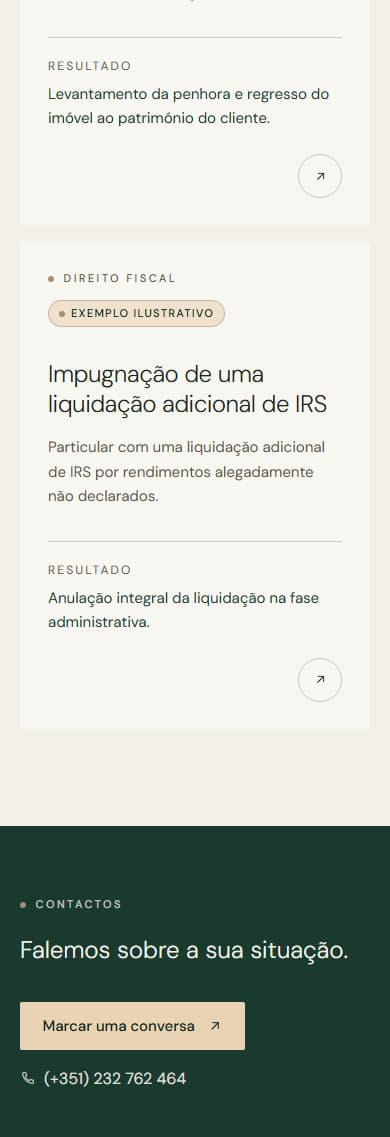
\includegraphics[width=0.235\textwidth]{screenshots/mobile/pt/casos-2.jpg}\hspace{0.012\textwidth}
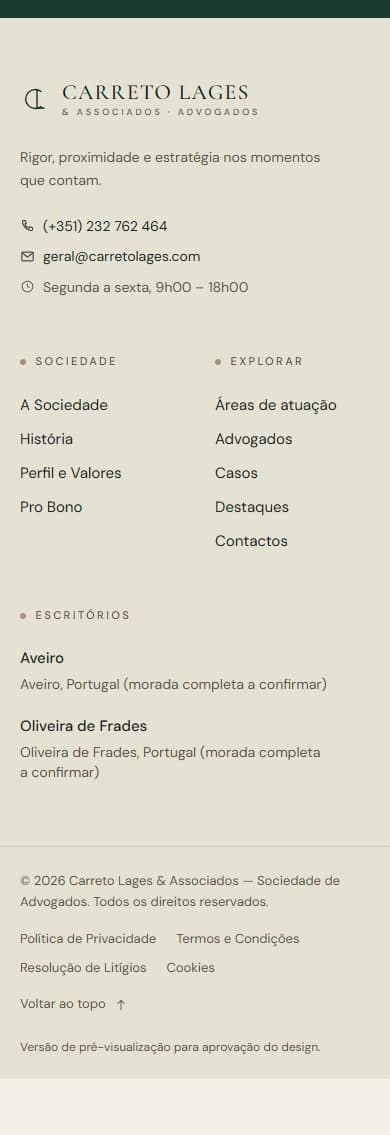
\includegraphics[width=0.235\textwidth]{screenshots/mobile/pt/casos-3.jpg}\par\medskip
\bigskip
\needspace{8\baselineskip}
\subsection*{Absolvição num processo de burla informática}
\addcontentsline{toc}{subsection}{Absolvição num processo de burla informática (\texttt{/casos/absolvicao-burla-informatica})}
\noindent{\small\color{tintasuave}\texttt{/casos/absolvicao-burla-informatica}}\par\smallskip
\noindent{\footnotesize Computador (1440\,px)}\par\smallskip
\noindent 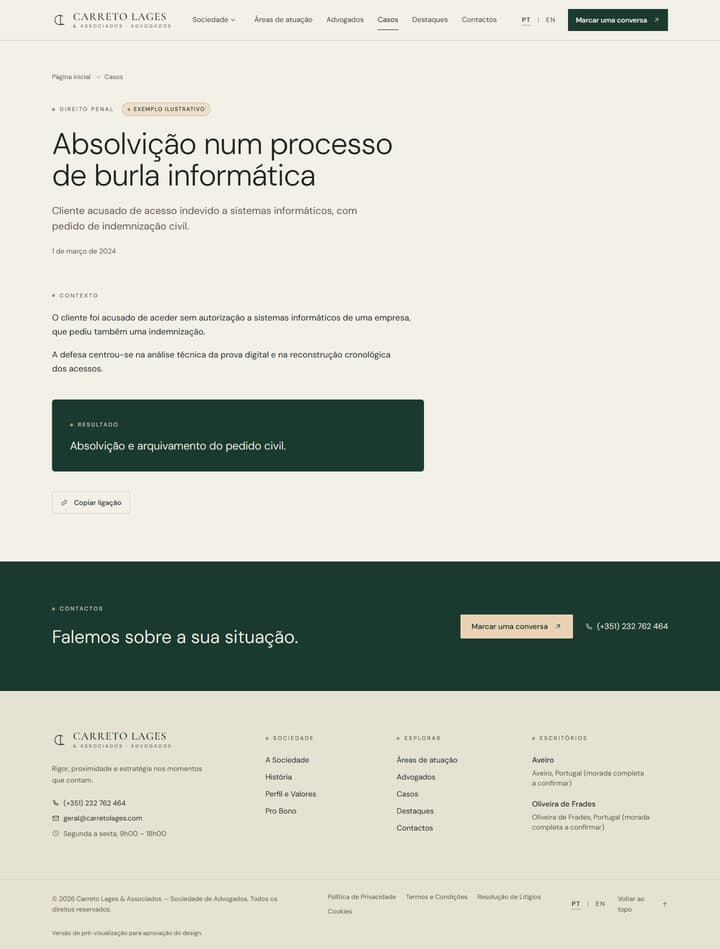
\includegraphics[width=0.485\textwidth]{screenshots/desktop/pt/casos--absolvicao-burla-informatica.jpg}\par\medskip
\noindent{\footnotesize Telemóvel (390\,px)}\par\smallskip
\noindent 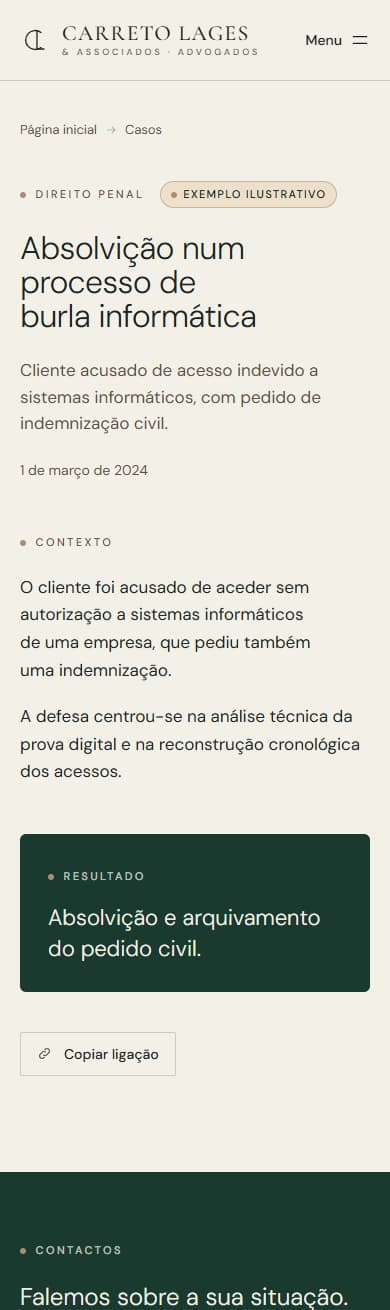
\includegraphics[width=0.235\textwidth]{screenshots/mobile/pt/casos--absolvicao-burla-informatica-1.jpg}\hspace{0.012\textwidth}
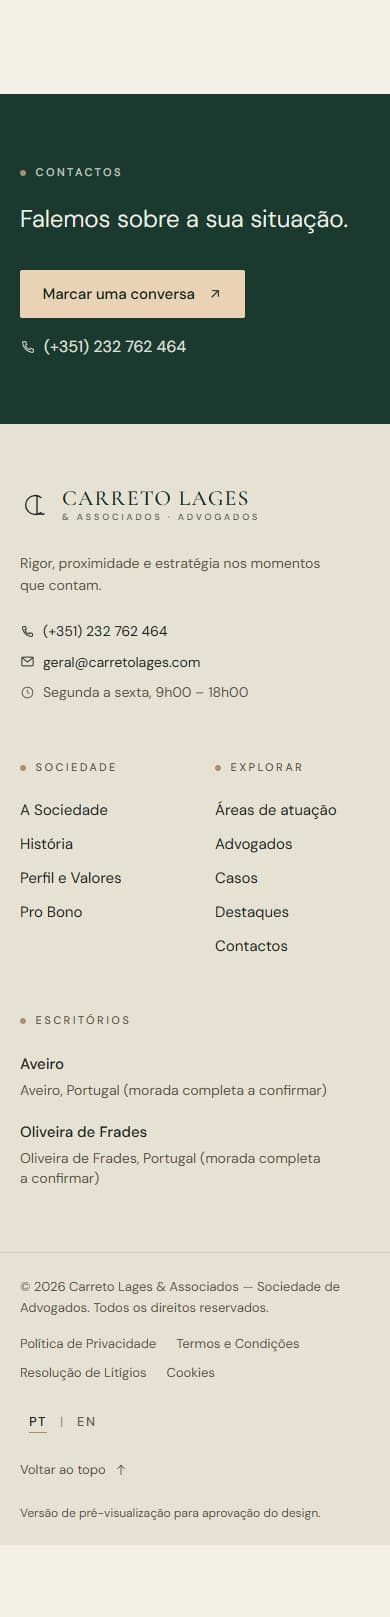
\includegraphics[width=0.235\textwidth]{screenshots/mobile/pt/casos--absolvicao-burla-informatica-2.jpg}\par\medskip
\bigskip
\needspace{8\baselineskip}
\subsection*{Impugnação de uma liquidação adicional de IRS}
\addcontentsline{toc}{subsection}{Impugnação de uma liquidação adicional de IRS (\texttt{/casos/impugnacao-liquidacao-irs})}
\noindent{\small\color{tintasuave}\texttt{/casos/impugnacao-liquidacao-irs}}\par\smallskip
\noindent{\footnotesize Computador (1440\,px)}\par\smallskip
\noindent 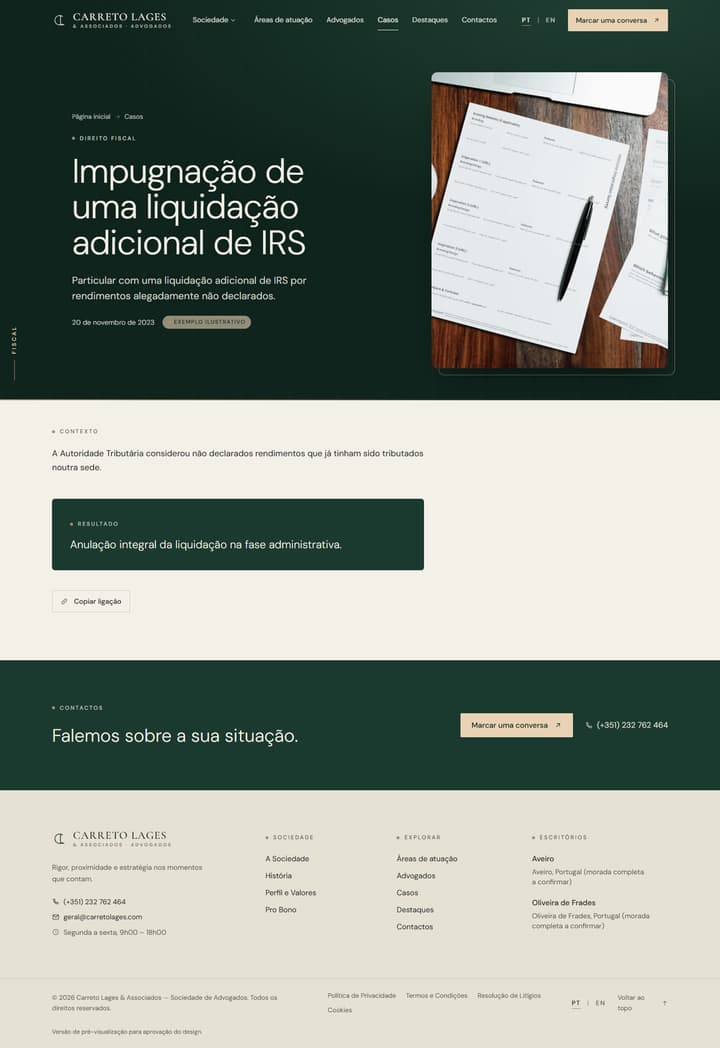
\includegraphics[width=0.485\textwidth]{screenshots/desktop/pt/casos--impugnacao-liquidacao-irs.jpg}\par\medskip
\noindent{\footnotesize Telemóvel (390\,px)}\par\smallskip
\noindent 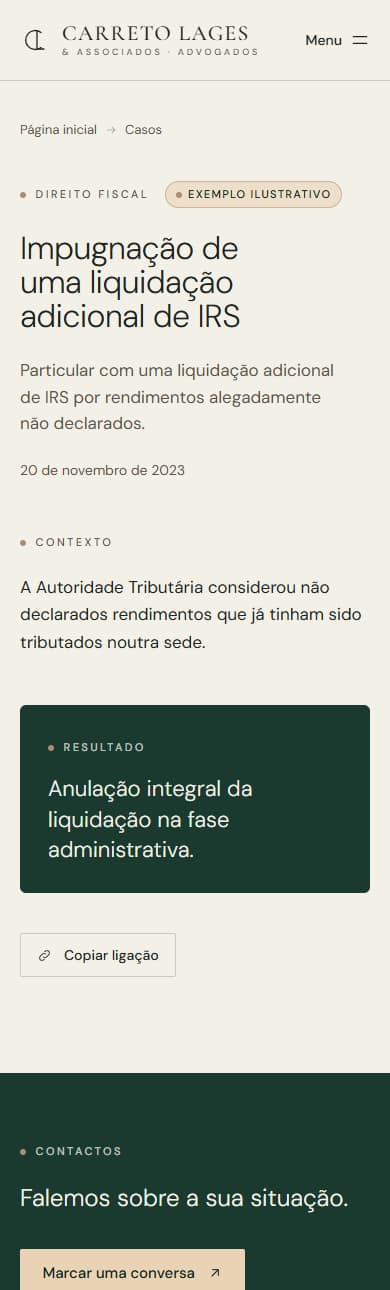
\includegraphics[width=0.235\textwidth]{screenshots/mobile/pt/casos--impugnacao-liquidacao-irs-1.jpg}\hspace{0.012\textwidth}
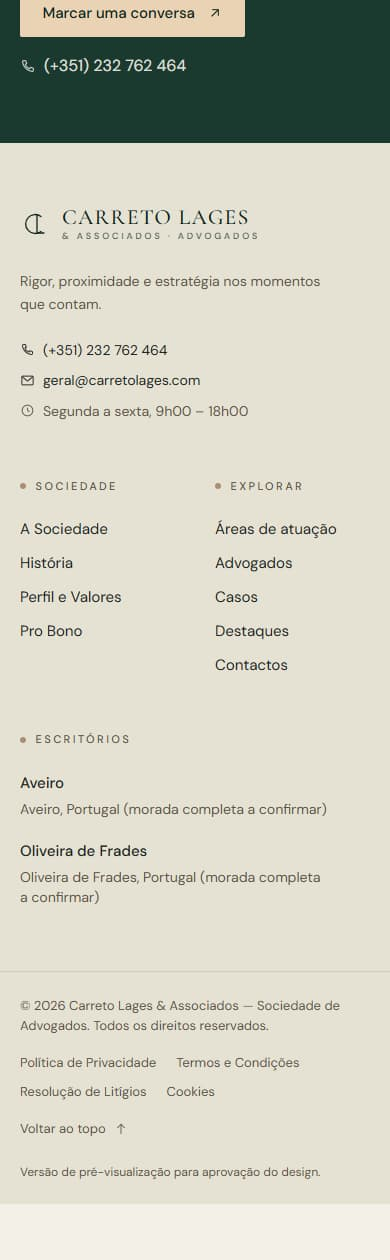
\includegraphics[width=0.235\textwidth]{screenshots/mobile/pt/casos--impugnacao-liquidacao-irs-2.jpg}\par\medskip
\bigskip
\needspace{8\baselineskip}
\subsection*{Recuperação de um imóvel num processo de insolvência}
\addcontentsline{toc}{subsection}{Recuperação de um imóvel num processo de insolvência (\texttt{/casos/recuperacao-imovel-insolvencia})}
\noindent{\small\color{tintasuave}\texttt{/casos/recuperacao-imovel-insolvencia}}\par\smallskip
\noindent{\footnotesize Computador (1440\,px)}\par\smallskip
\noindent 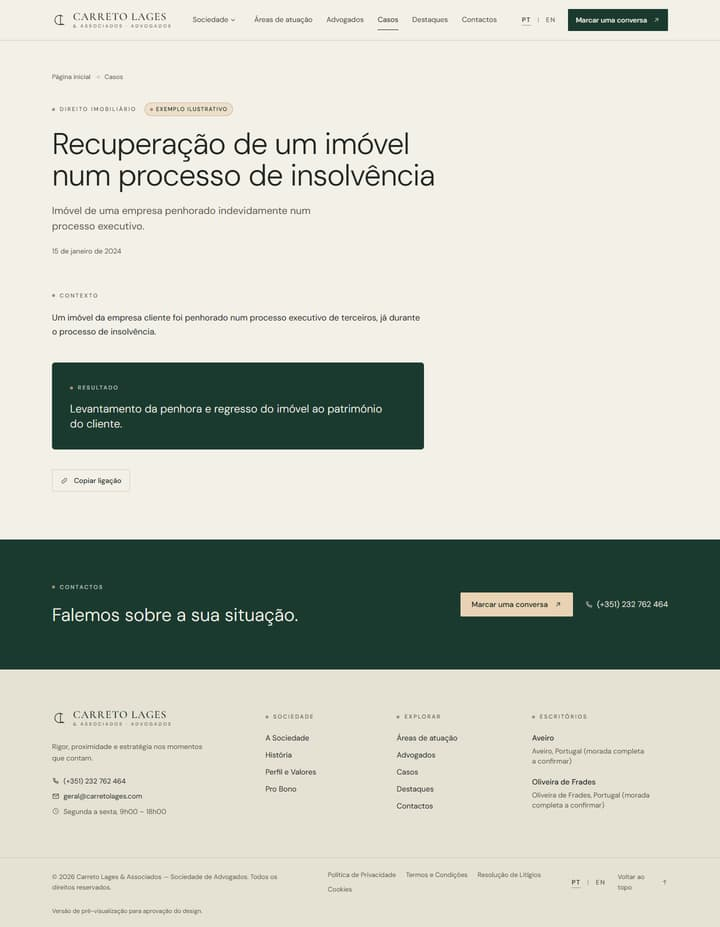
\includegraphics[width=0.485\textwidth]{screenshots/desktop/pt/casos--recuperacao-imovel-insolvencia.jpg}\par\medskip
\noindent{\footnotesize Telemóvel (390\,px)}\par\smallskip
\noindent 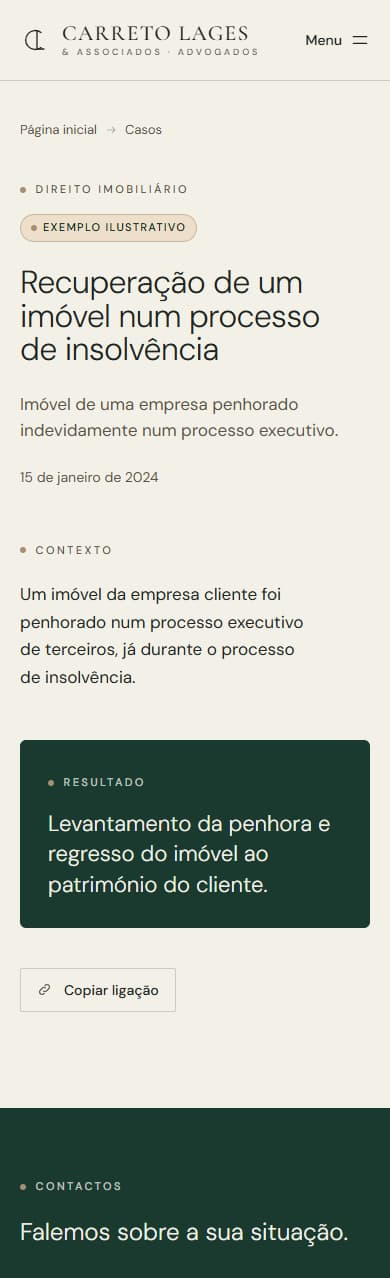
\includegraphics[width=0.235\textwidth]{screenshots/mobile/pt/casos--recuperacao-imovel-insolvencia-1.jpg}\hspace{0.012\textwidth}
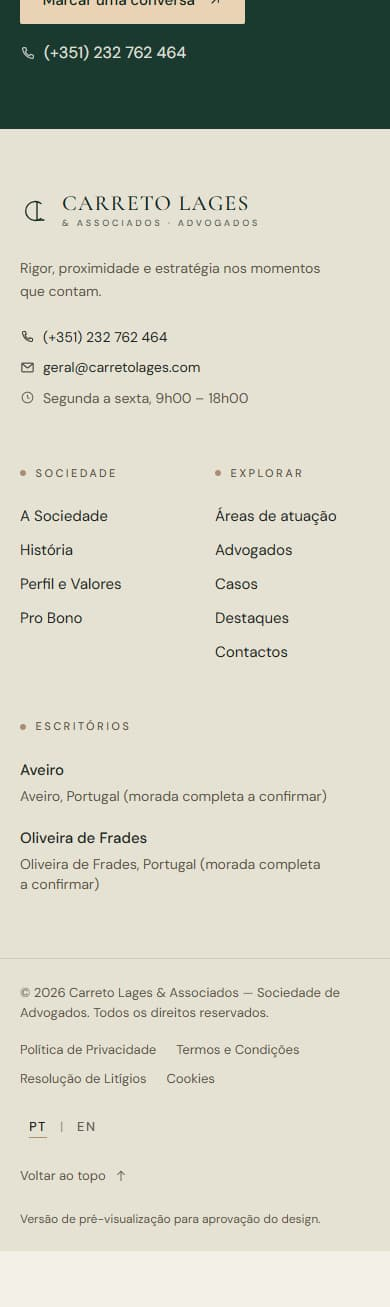
\includegraphics[width=0.235\textwidth]{screenshots/mobile/pt/casos--recuperacao-imovel-insolvencia-2.jpg}\par\medskip
\bigskip
\needspace{8\baselineskip}
\subsection*{Fale connosco.}
\addcontentsline{toc}{subsection}{Fale connosco. (\texttt{/contactos})}
\noindent{\small\color{tintasuave}\texttt{/contactos}}\par\smallskip
\noindent{\footnotesize Computador (1440\,px)}\par\smallskip
\noindent 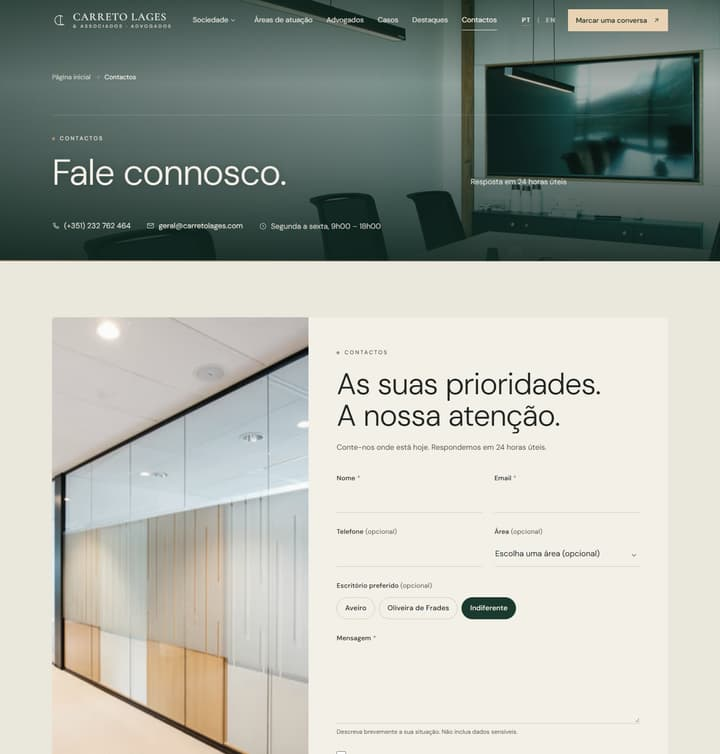
\includegraphics[width=0.485\textwidth]{screenshots/desktop/pt/contactos-1.jpg}\hspace{0.012\textwidth}
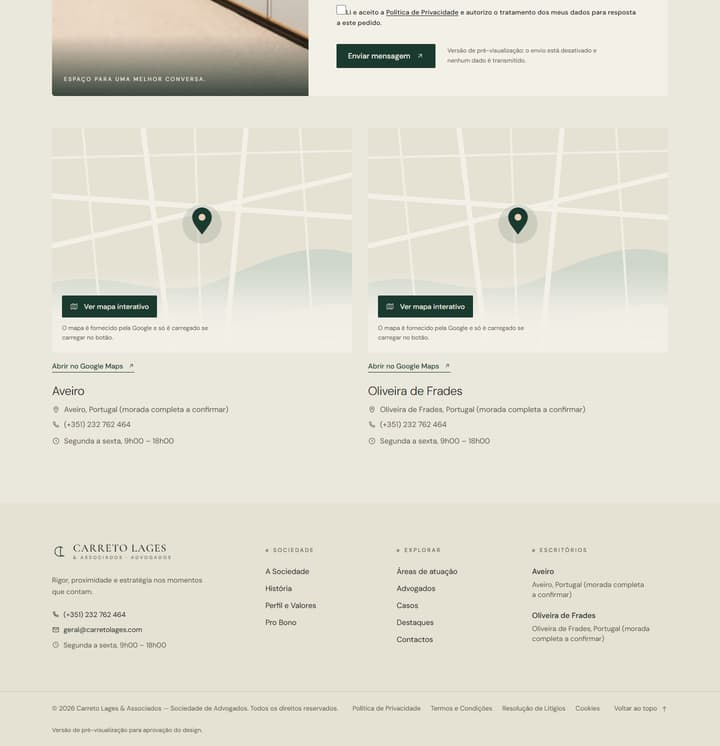
\includegraphics[width=0.485\textwidth]{screenshots/desktop/pt/contactos-2.jpg}\par\medskip
\noindent{\footnotesize Telemóvel (390\,px)}\par\smallskip
\noindent 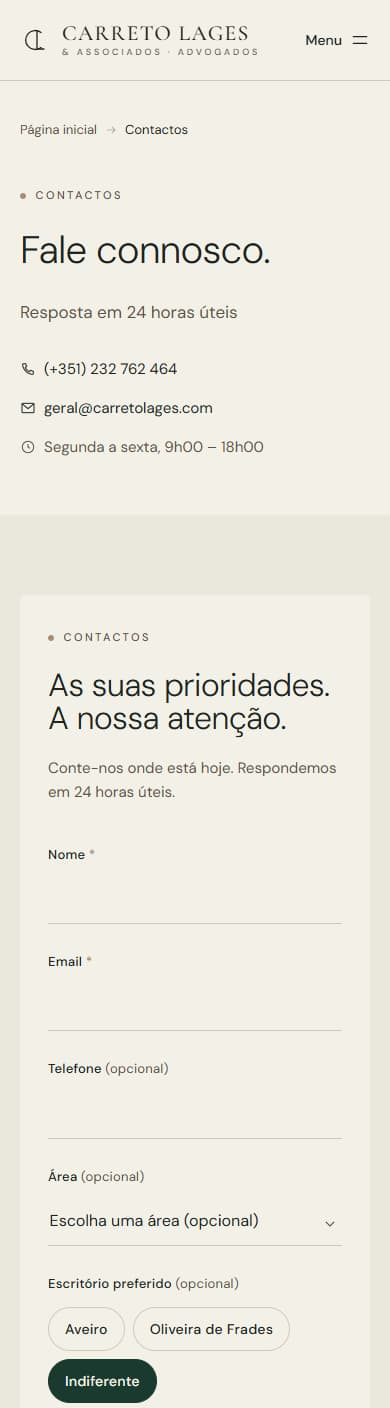
\includegraphics[width=0.235\textwidth]{screenshots/mobile/pt/contactos-1.jpg}\hspace{0.012\textwidth}
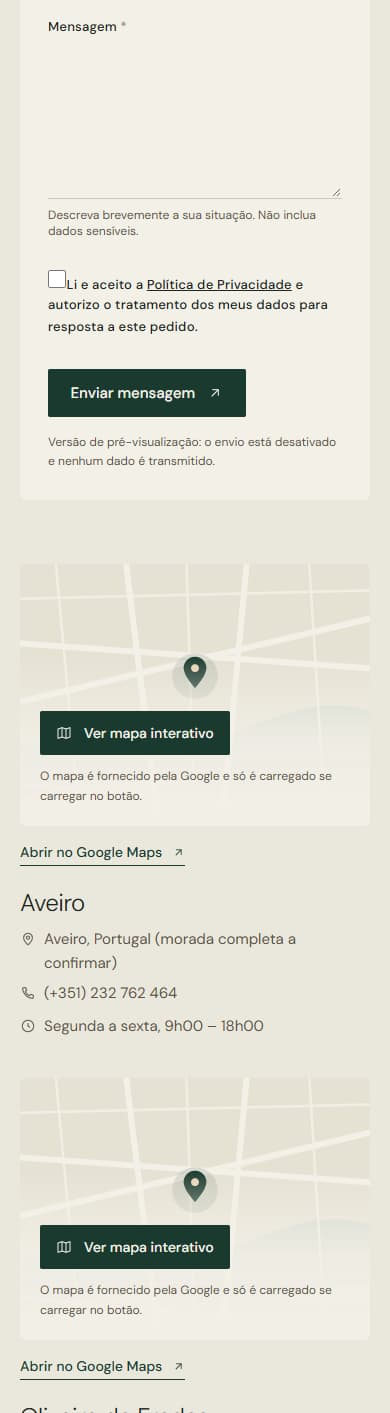
\includegraphics[width=0.235\textwidth]{screenshots/mobile/pt/contactos-2.jpg}\hspace{0.012\textwidth}
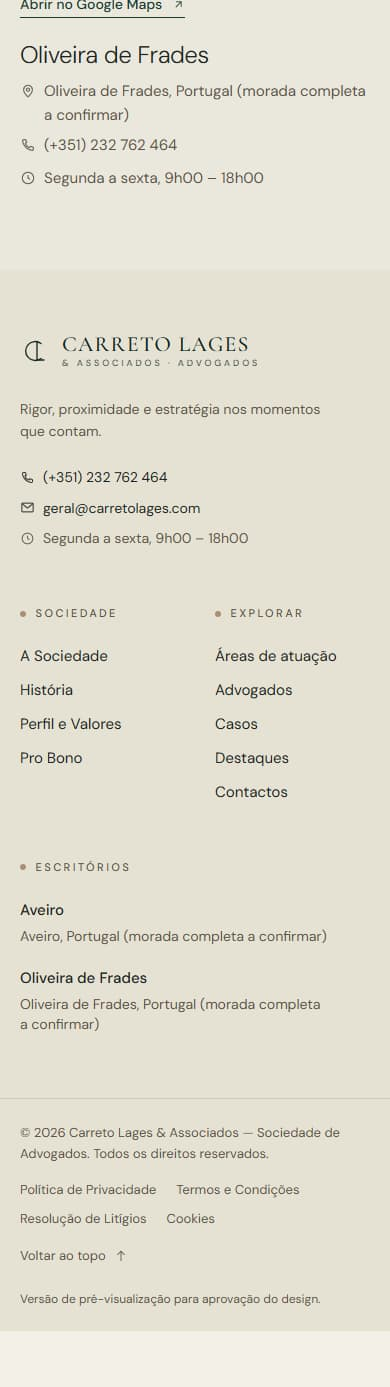
\includegraphics[width=0.235\textwidth]{screenshots/mobile/pt/contactos-3.jpg}\par\medskip
\bigskip
\needspace{8\baselineskip}
\subsection*{Este site não usa cookies.}
\addcontentsline{toc}{subsection}{Este site não usa cookies. (\texttt{/cookies})}
\noindent{\small\color{tintasuave}\texttt{/cookies}}\par\smallskip
\noindent{\footnotesize Computador (1440\,px)}\par\smallskip
\noindent 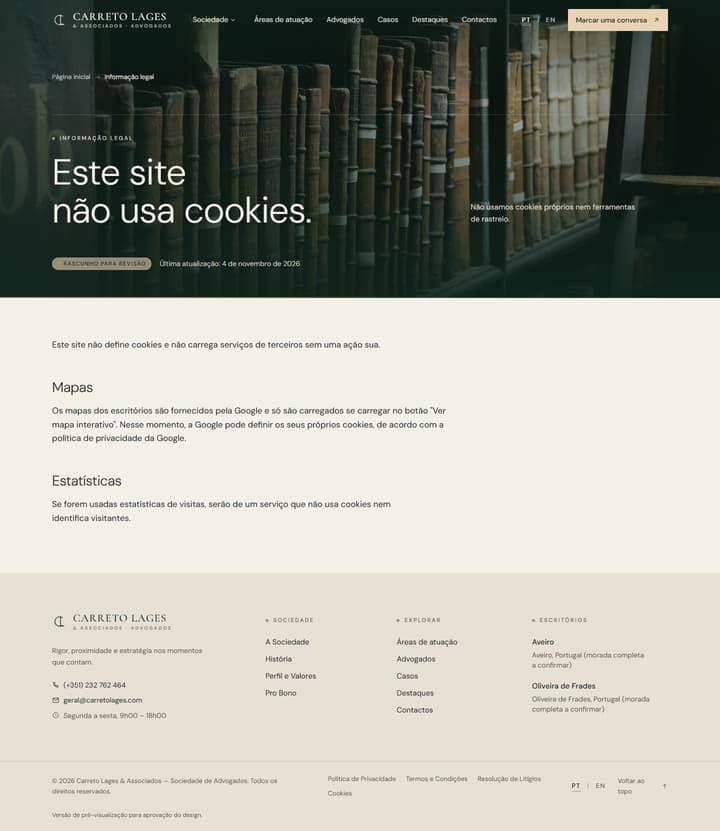
\includegraphics[width=0.485\textwidth]{screenshots/desktop/pt/cookies.jpg}\par\medskip
\noindent{\footnotesize Telemóvel (390\,px)}\par\smallskip
\noindent 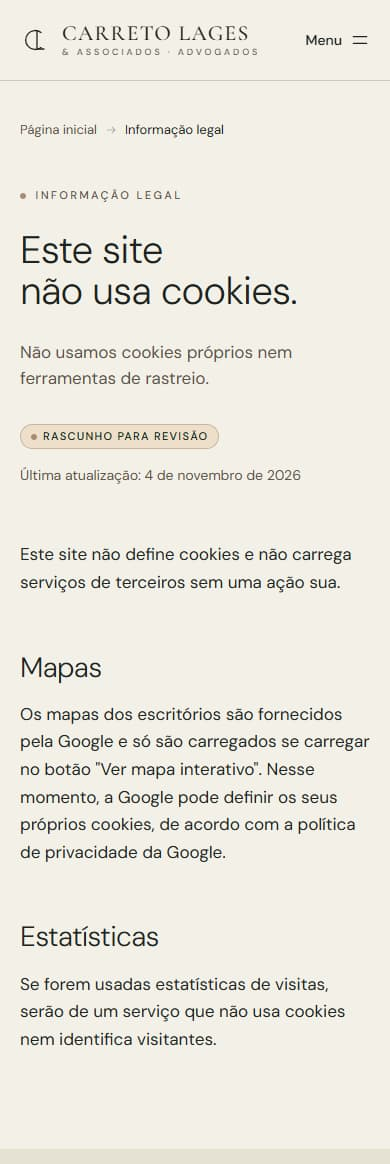
\includegraphics[width=0.235\textwidth]{screenshots/mobile/pt/cookies-1.jpg}\hspace{0.012\textwidth}
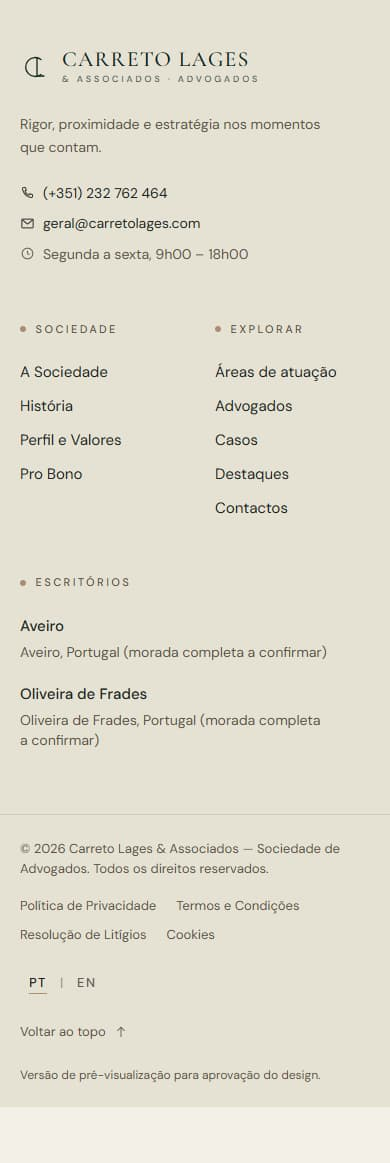
\includegraphics[width=0.235\textwidth]{screenshots/mobile/pt/cookies-2.jpg}\par\medskip
\bigskip
\needspace{8\baselineskip}
\subsection*{Notas claras sobre o que muda.}
\addcontentsline{toc}{subsection}{Notas claras sobre o que muda. (\texttt{/destaques})}
\noindent{\small\color{tintasuave}\texttt{/destaques}}\par\smallskip
\noindent{\footnotesize Computador (1440\,px)}\par\smallskip
\noindent 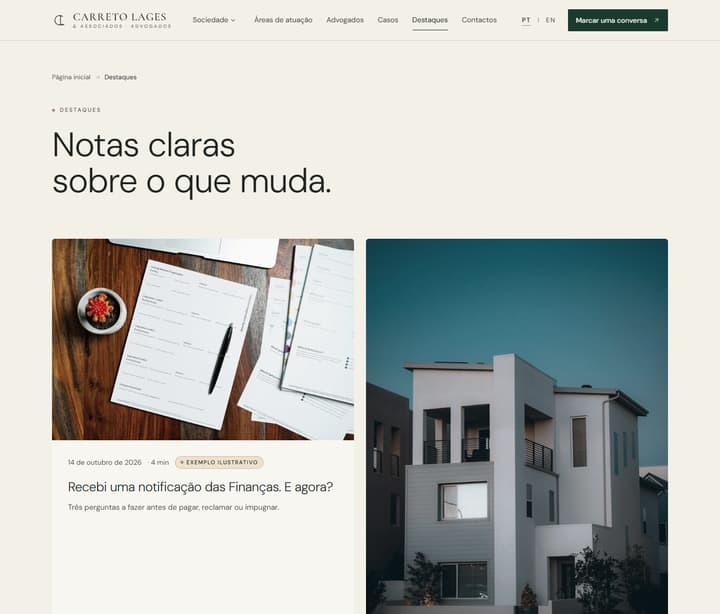
\includegraphics[width=0.485\textwidth]{screenshots/desktop/pt/destaques-1.jpg}\hspace{0.012\textwidth}
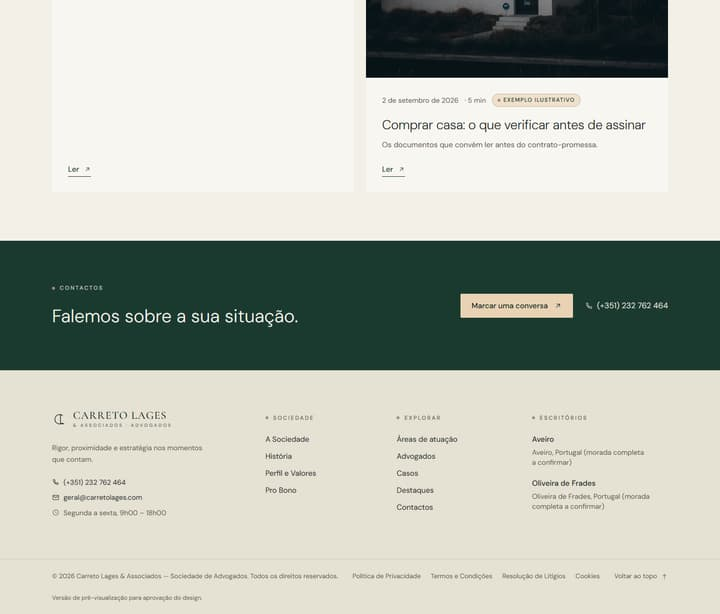
\includegraphics[width=0.485\textwidth]{screenshots/desktop/pt/destaques-2.jpg}\par\medskip
\noindent{\footnotesize Telemóvel (390\,px)}\par\smallskip
\noindent 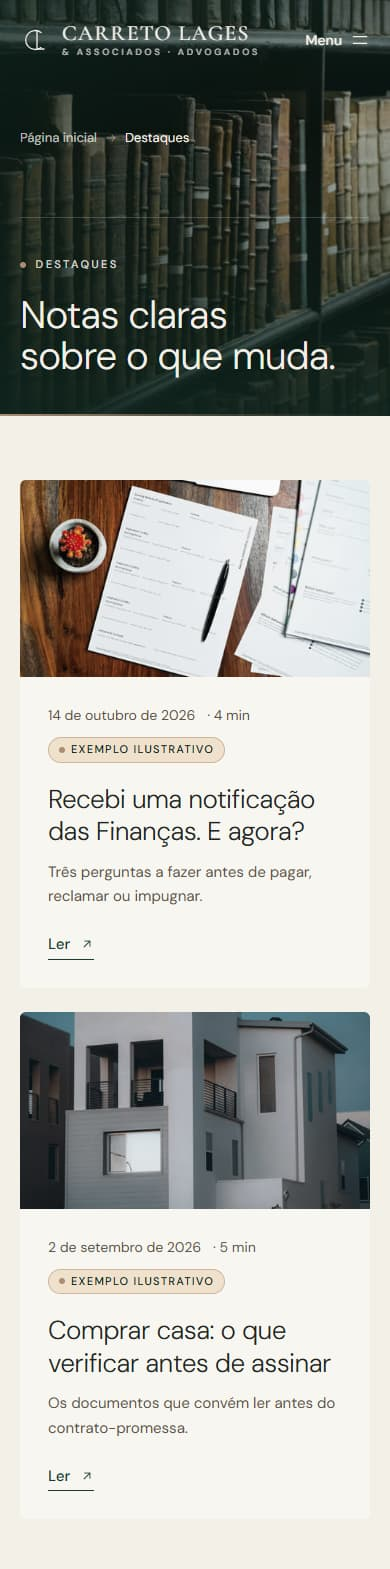
\includegraphics[width=0.235\textwidth]{screenshots/mobile/pt/destaques-1.jpg}\hspace{0.012\textwidth}
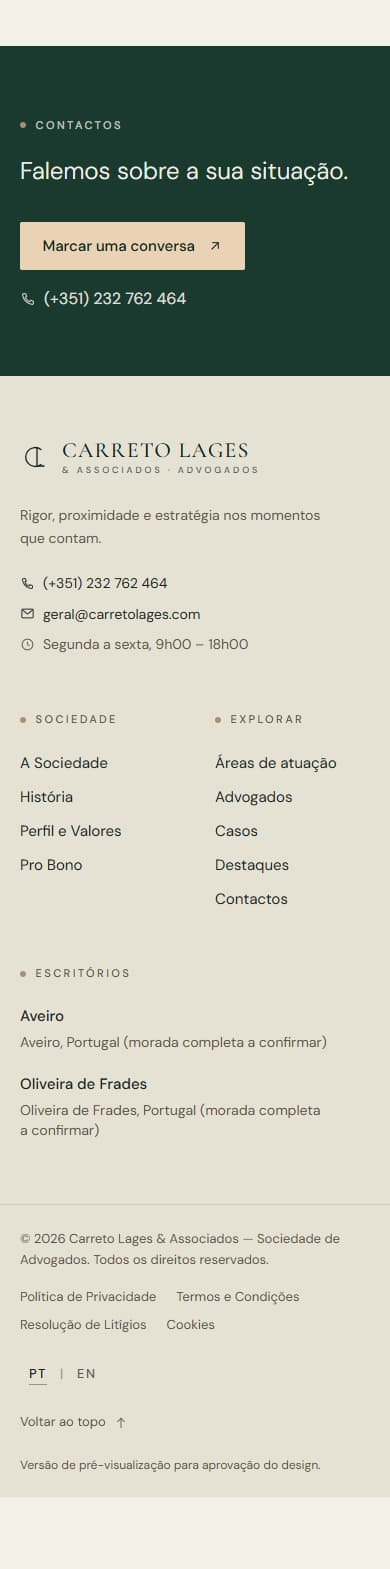
\includegraphics[width=0.235\textwidth]{screenshots/mobile/pt/destaques-2.jpg}\par\medskip
\bigskip
\needspace{8\baselineskip}
\subsection*{Comprar casa: o que verificar antes de assinar}
\addcontentsline{toc}{subsection}{Comprar casa: o que verificar antes de assinar (\texttt{/destaques/comprar-casa-antes-de-assinar})}
\noindent{\small\color{tintasuave}\texttt{/destaques/comprar-casa-antes-de-assinar}}\par\smallskip
\noindent{\footnotesize Computador (1440\,px)}\par\smallskip
\noindent 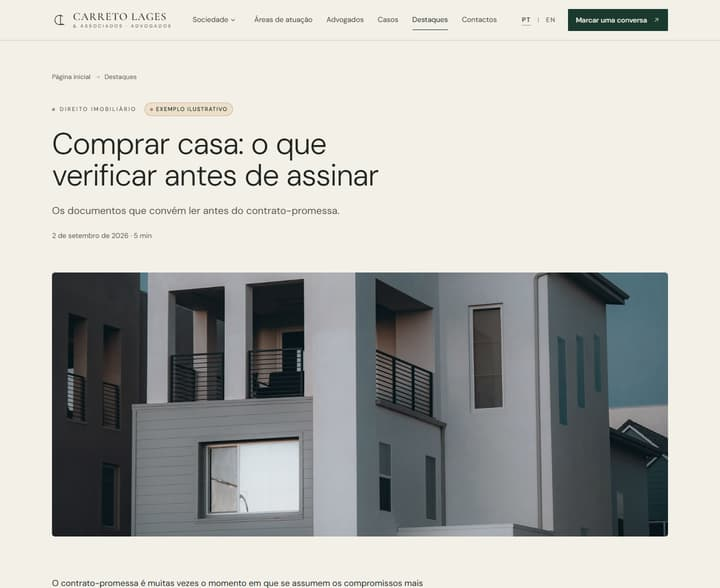
\includegraphics[width=0.485\textwidth]{screenshots/desktop/pt/destaques--comprar-casa-antes-de-assinar-1.jpg}\hspace{0.012\textwidth}
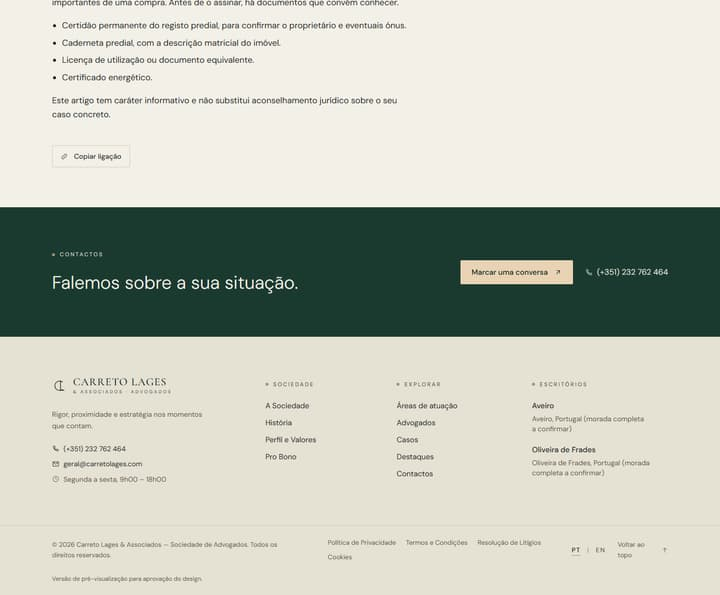
\includegraphics[width=0.485\textwidth]{screenshots/desktop/pt/destaques--comprar-casa-antes-de-assinar-2.jpg}\par\medskip
\noindent{\footnotesize Telemóvel (390\,px)}\par\smallskip
\noindent 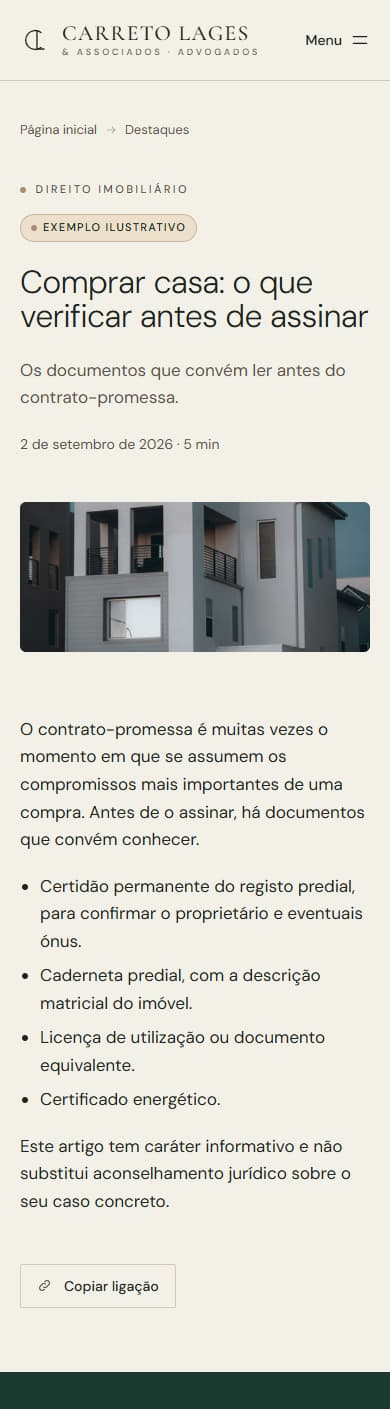
\includegraphics[width=0.235\textwidth]{screenshots/mobile/pt/destaques--comprar-casa-antes-de-assinar-1.jpg}\hspace{0.012\textwidth}
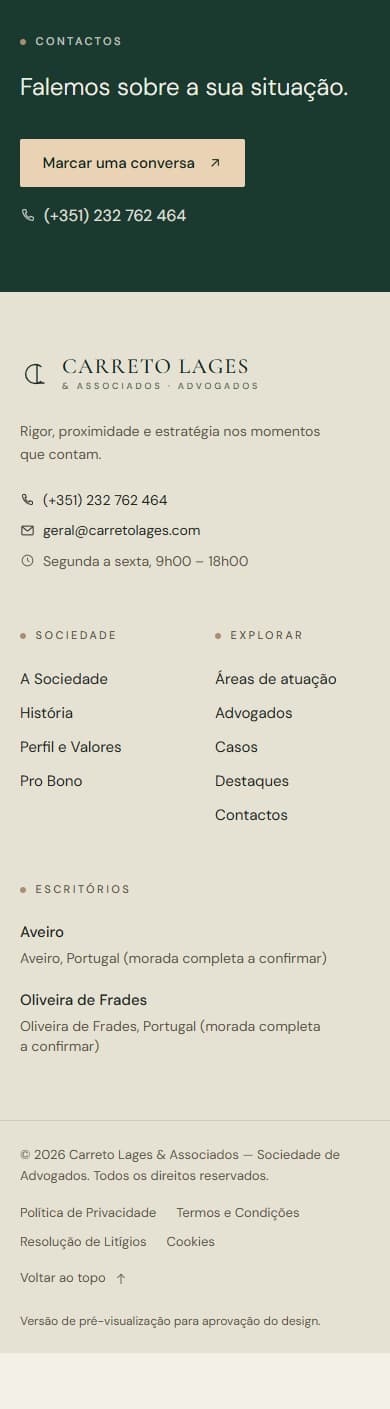
\includegraphics[width=0.235\textwidth]{screenshots/mobile/pt/destaques--comprar-casa-antes-de-assinar-2.jpg}\par\medskip
\bigskip
\needspace{8\baselineskip}
\subsection*{Recebi uma notificação das Finanças. E agora?}
\addcontentsline{toc}{subsection}{Recebi uma notificação das Finanças. E agora? (\texttt{/destaques/recebi-uma-notificacao-das-financas})}
\noindent{\small\color{tintasuave}\texttt{/destaques/recebi-uma-notificacao-das-financas}}\par\smallskip
\noindent{\footnotesize Computador (1440\,px)}\par\smallskip
\noindent 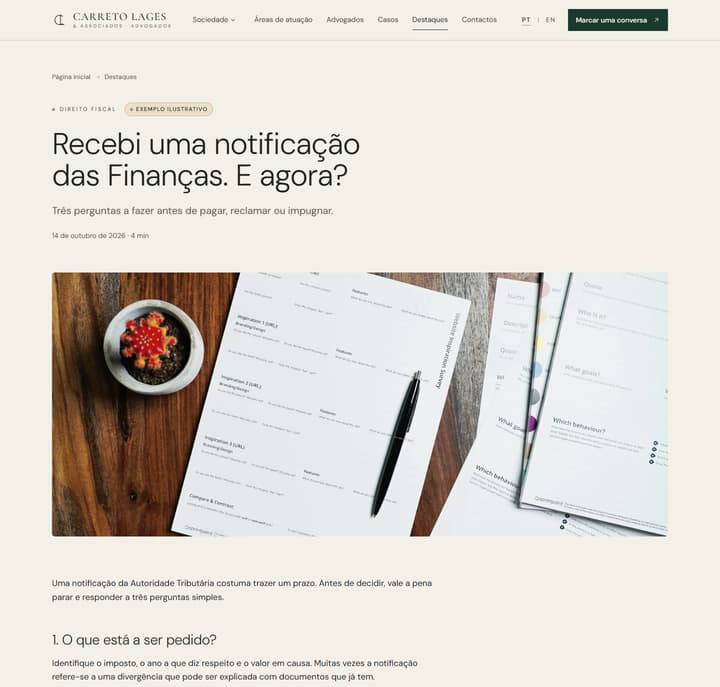
\includegraphics[width=0.485\textwidth]{screenshots/desktop/pt/destaques--recebi-uma-notificacao-das-financas-1.jpg}\hspace{0.012\textwidth}
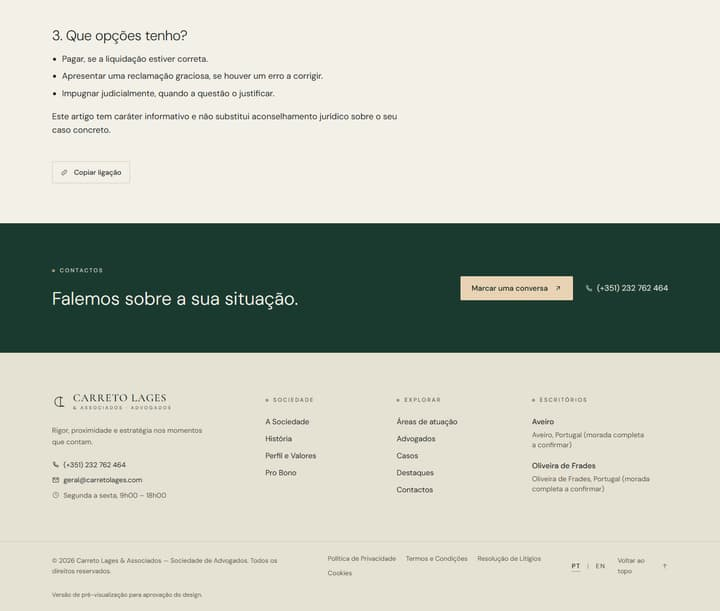
\includegraphics[width=0.485\textwidth]{screenshots/desktop/pt/destaques--recebi-uma-notificacao-das-financas-2.jpg}\par\medskip
\noindent{\footnotesize Telemóvel (390\,px)}\par\smallskip
\noindent 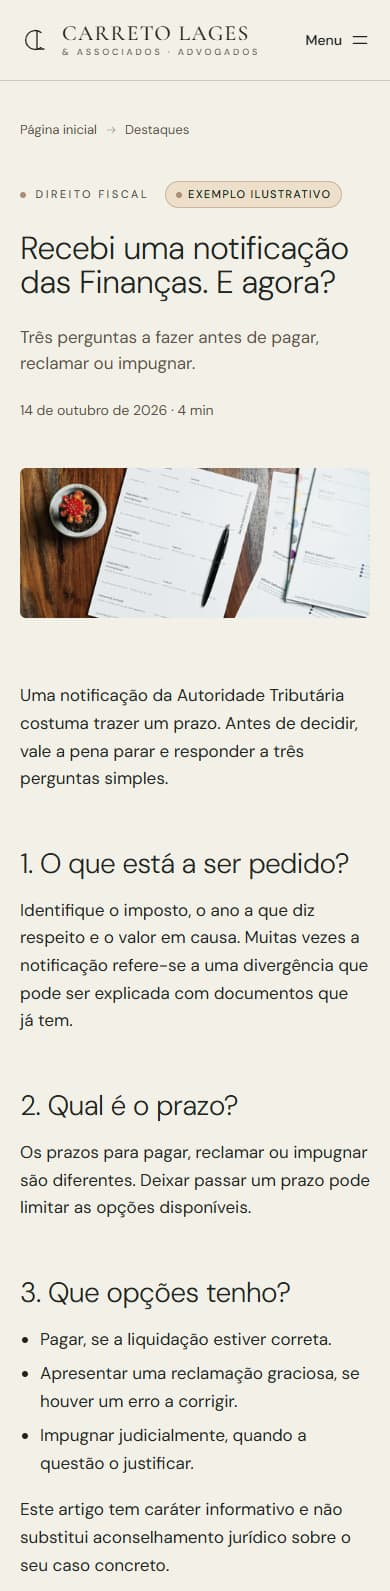
\includegraphics[width=0.235\textwidth]{screenshots/mobile/pt/destaques--recebi-uma-notificacao-das-financas-1.jpg}\hspace{0.012\textwidth}
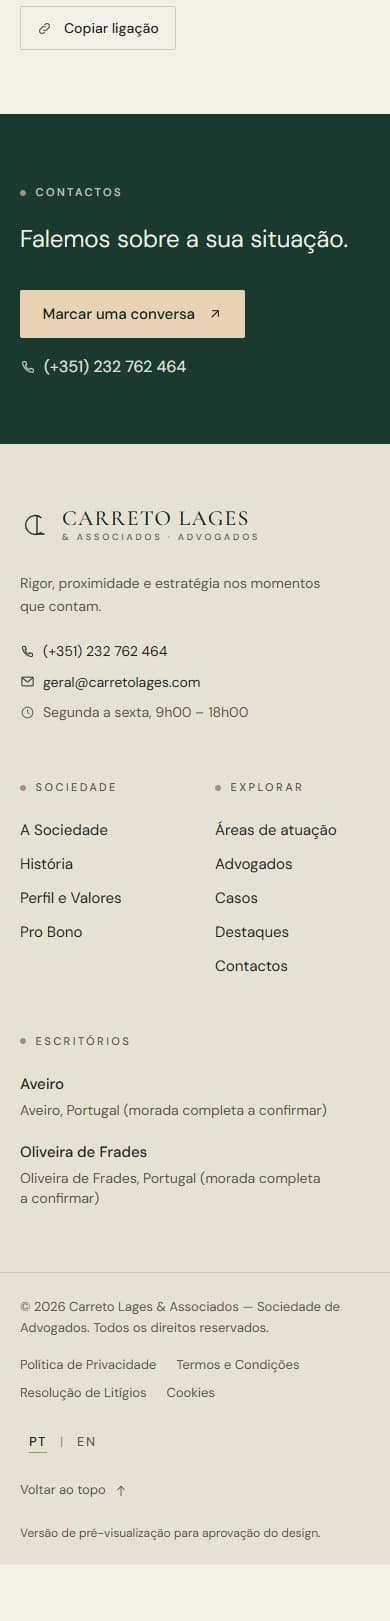
\includegraphics[width=0.235\textwidth]{screenshots/mobile/pt/destaques--recebi-uma-notificacao-das-financas-2.jpg}\par\medskip
\bigskip
\needspace{8\baselineskip}
\subsection*{Obrigado. Recebemos a sua mensagem.}
\addcontentsline{toc}{subsection}{Obrigado. Recebemos a sua mensagem. (\texttt{/obrigado})}
\noindent{\small\color{tintasuave}\texttt{/obrigado}}\par\smallskip
\noindent{\footnotesize Computador (1440\,px)}\par\smallskip
\noindent 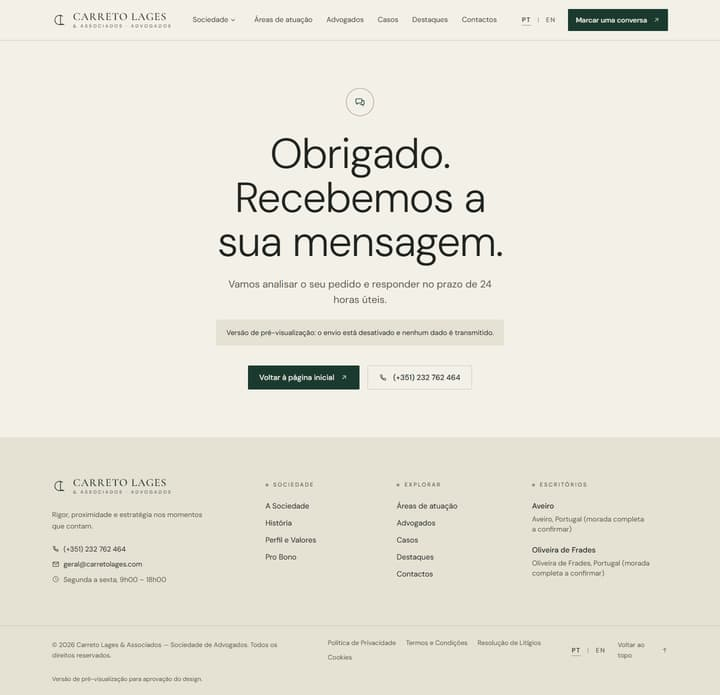
\includegraphics[width=0.485\textwidth]{screenshots/desktop/pt/obrigado.jpg}\par\medskip
\noindent{\footnotesize Telemóvel (390\,px)}\par\smallskip
\noindent 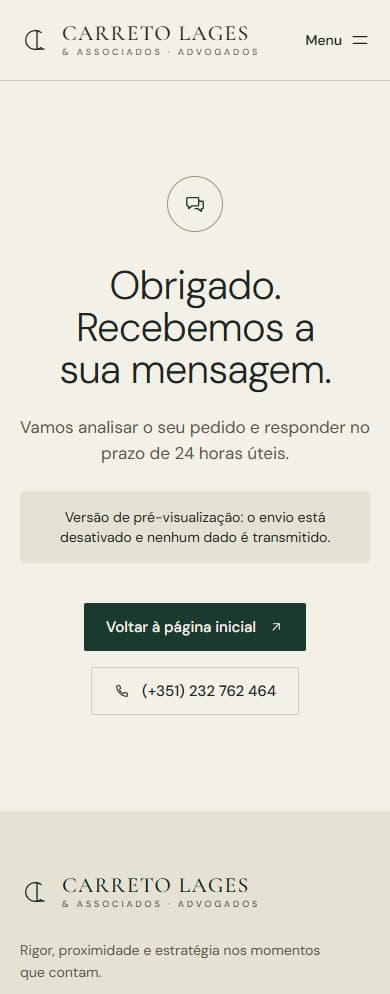
\includegraphics[width=0.235\textwidth]{screenshots/mobile/pt/obrigado-1.jpg}\hspace{0.012\textwidth}
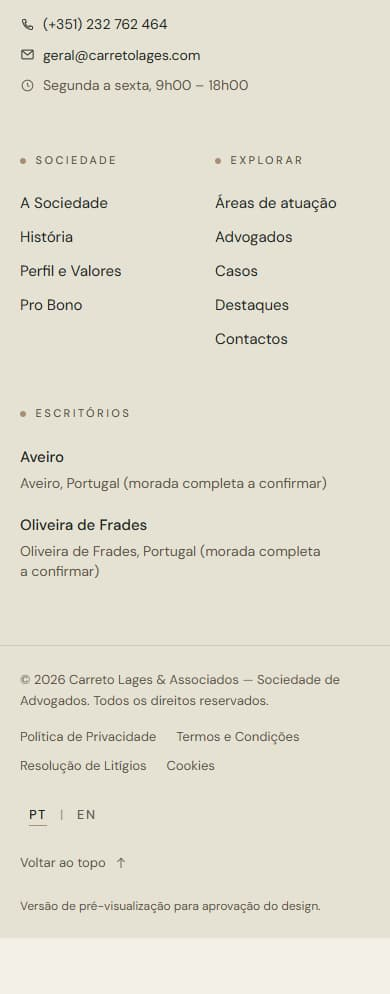
\includegraphics[width=0.235\textwidth]{screenshots/mobile/pt/obrigado-2.jpg}\par\medskip
\bigskip
\needspace{8\baselineskip}
\subsection*{Política de Privacidade}
\addcontentsline{toc}{subsection}{Política de Privacidade (\texttt{/politica-de-privacidade})}
\noindent{\small\color{tintasuave}\texttt{/politica-de-privacidade}}\par\smallskip
\noindent{\footnotesize Computador (1440\,px)}\par\smallskip
\noindent 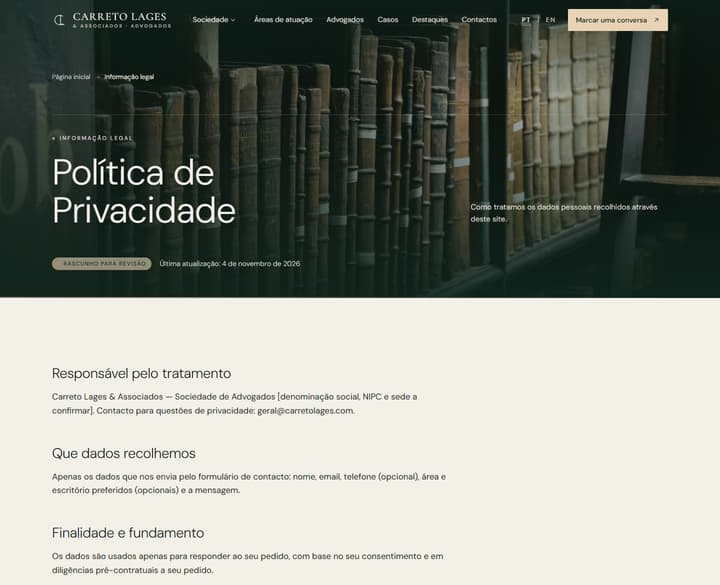
\includegraphics[width=0.485\textwidth]{screenshots/desktop/pt/politica-de-privacidade-1.jpg}\hspace{0.012\textwidth}
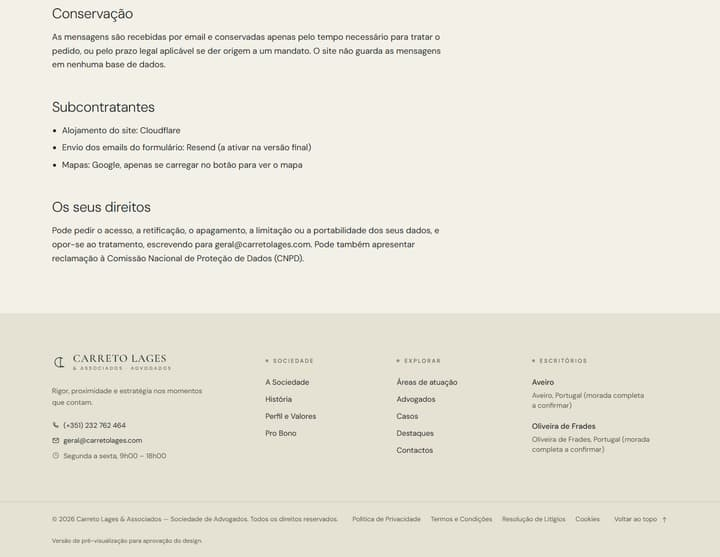
\includegraphics[width=0.485\textwidth]{screenshots/desktop/pt/politica-de-privacidade-2.jpg}\par\medskip
\noindent{\footnotesize Telemóvel (390\,px)}\par\smallskip
\noindent 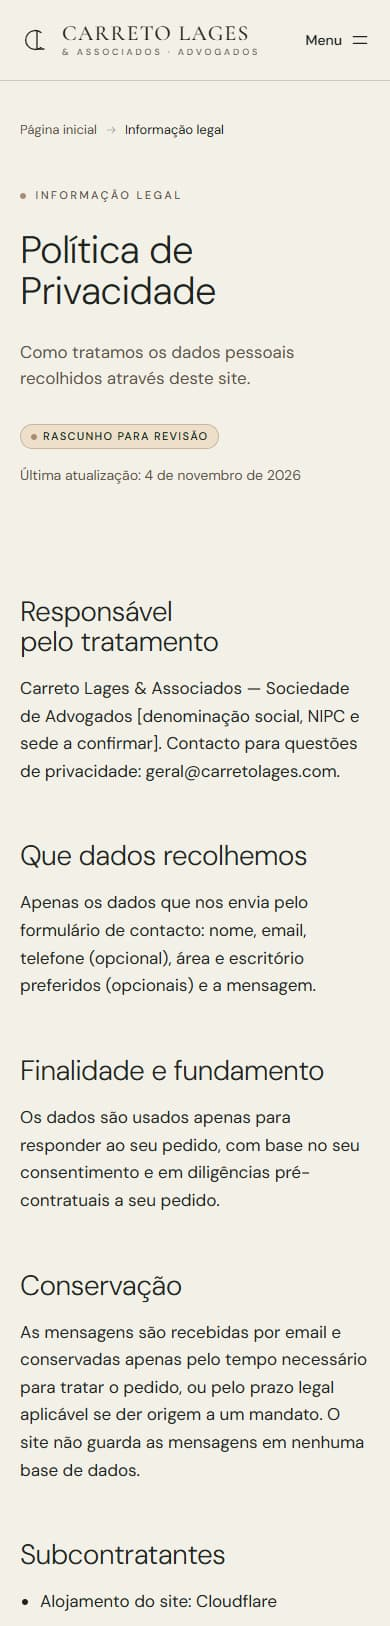
\includegraphics[width=0.235\textwidth]{screenshots/mobile/pt/politica-de-privacidade-1.jpg}\hspace{0.012\textwidth}
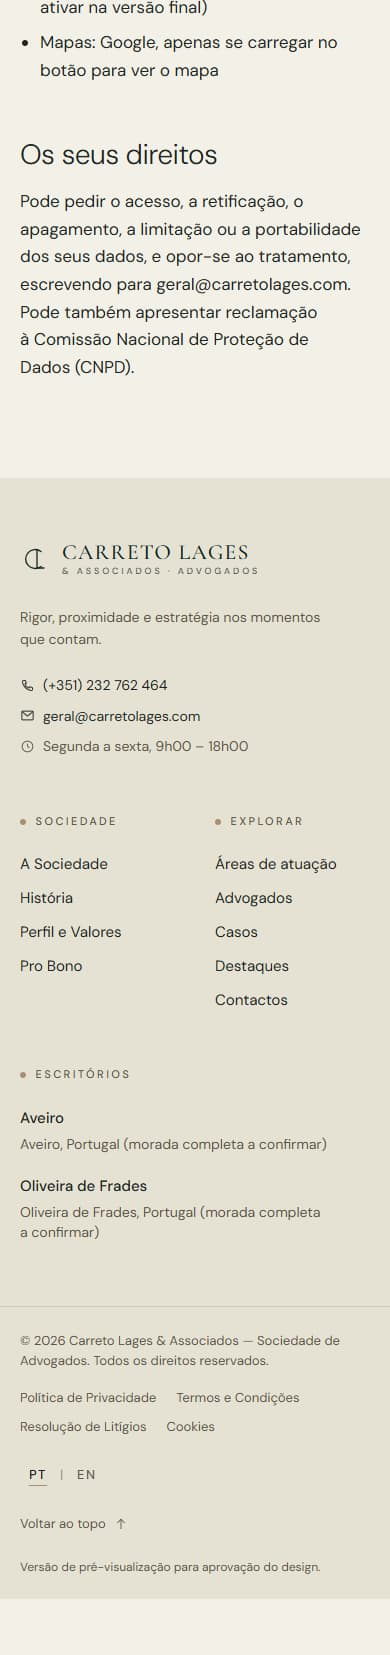
\includegraphics[width=0.235\textwidth]{screenshots/mobile/pt/politica-de-privacidade-2.jpg}\par\medskip
\bigskip
\needspace{8\baselineskip}
\subsection*{Resolução de Litígios}
\addcontentsline{toc}{subsection}{Resolução de Litígios (\texttt{/resolucao-de-litigios})}
\noindent{\small\color{tintasuave}\texttt{/resolucao-de-litigios}}\par\smallskip
\noindent{\footnotesize Computador (1440\,px)}\par\smallskip
\noindent 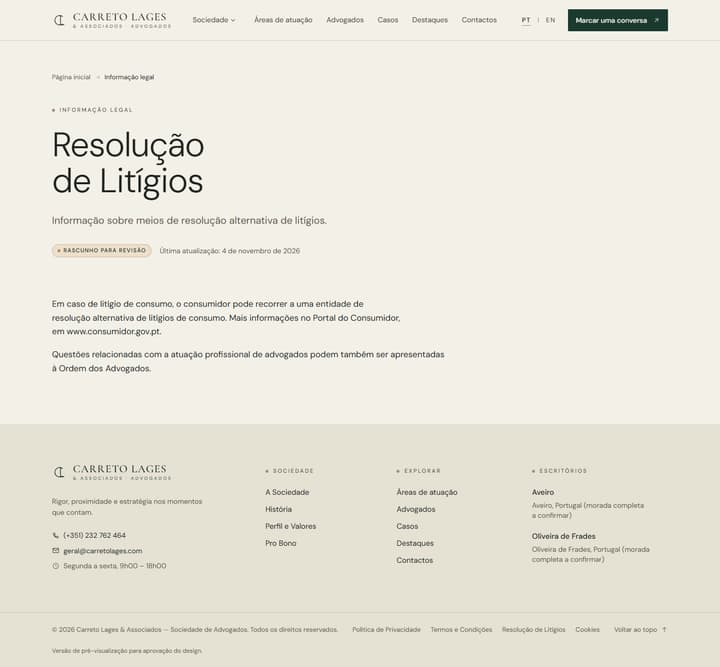
\includegraphics[width=0.485\textwidth]{screenshots/desktop/pt/resolucao-de-litigios.jpg}\par\medskip
\noindent{\footnotesize Telemóvel (390\,px)}\par\smallskip
\noindent 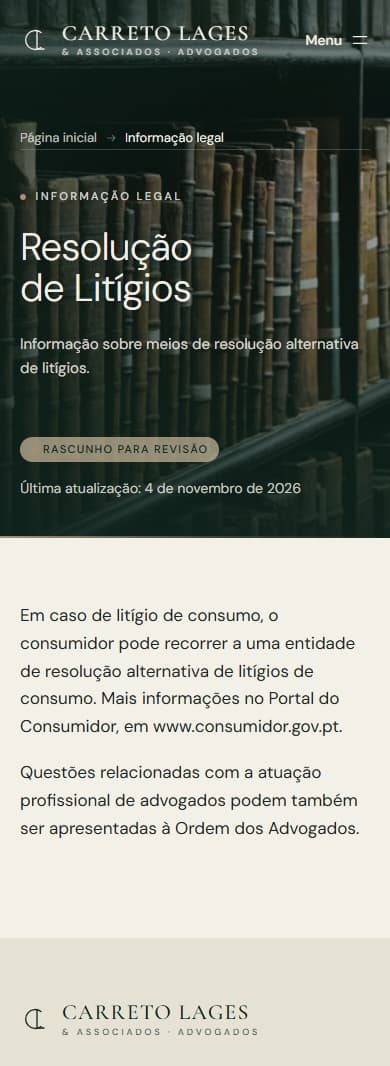
\includegraphics[width=0.235\textwidth]{screenshots/mobile/pt/resolucao-de-litigios-1.jpg}\hspace{0.012\textwidth}
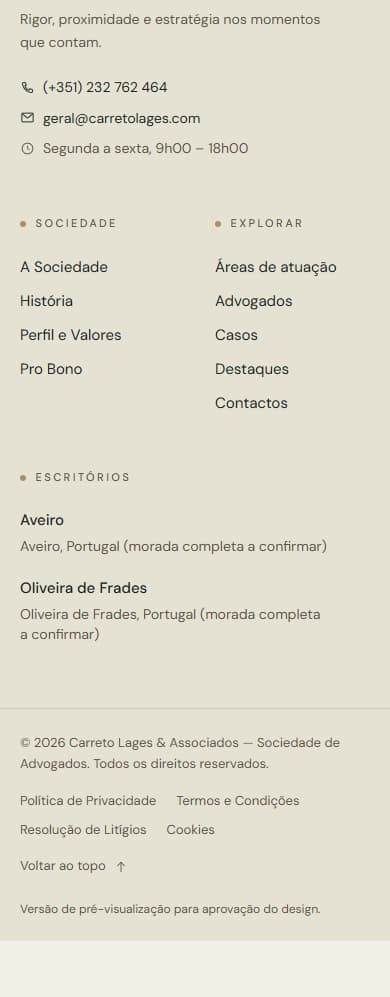
\includegraphics[width=0.235\textwidth]{screenshots/mobile/pt/resolucao-de-litigios-2.jpg}\par\medskip
\bigskip
\needspace{8\baselineskip}
\subsection*{Uma sociedade próxima, desde 2002.}
\addcontentsline{toc}{subsection}{Uma sociedade próxima, desde 2002. (\texttt{/sociedade})}
\noindent{\small\color{tintasuave}\texttt{/sociedade}}\par\smallskip
\noindent{\footnotesize Computador (1440\,px)}\par\smallskip
\noindent 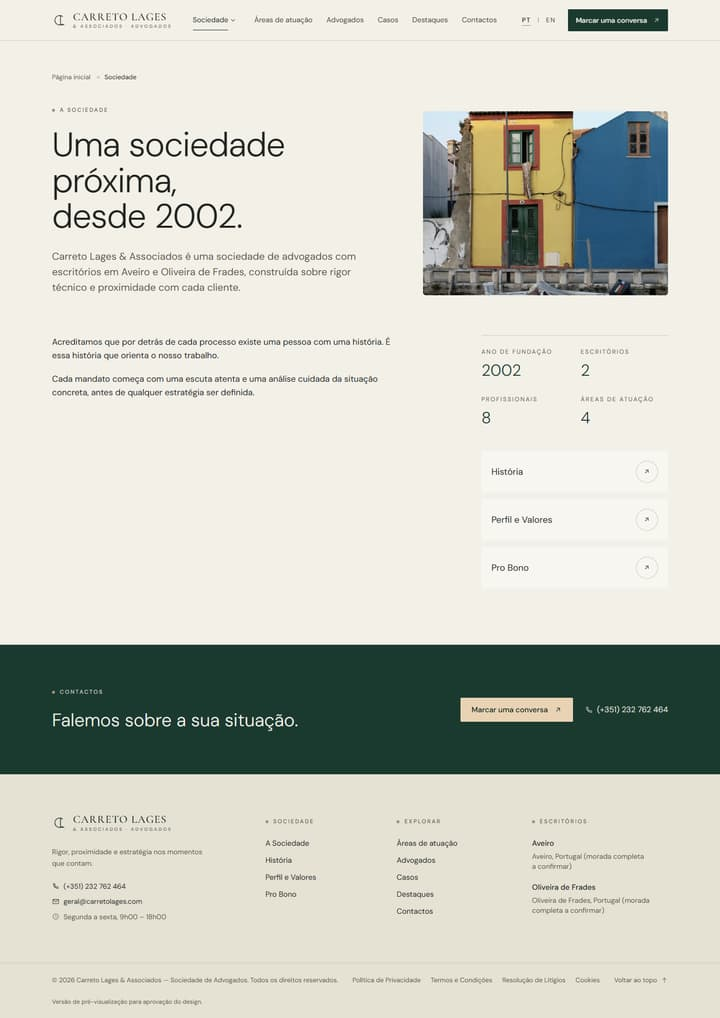
\includegraphics[width=0.485\textwidth]{screenshots/desktop/pt/sociedade.jpg}\par\medskip
\noindent{\footnotesize Telemóvel (390\,px)}\par\smallskip
\noindent 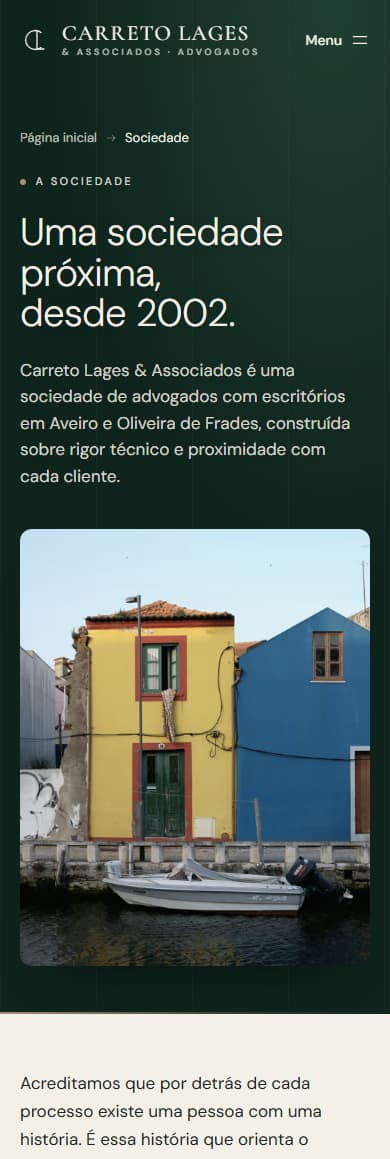
\includegraphics[width=0.235\textwidth]{screenshots/mobile/pt/sociedade-1.jpg}\hspace{0.012\textwidth}
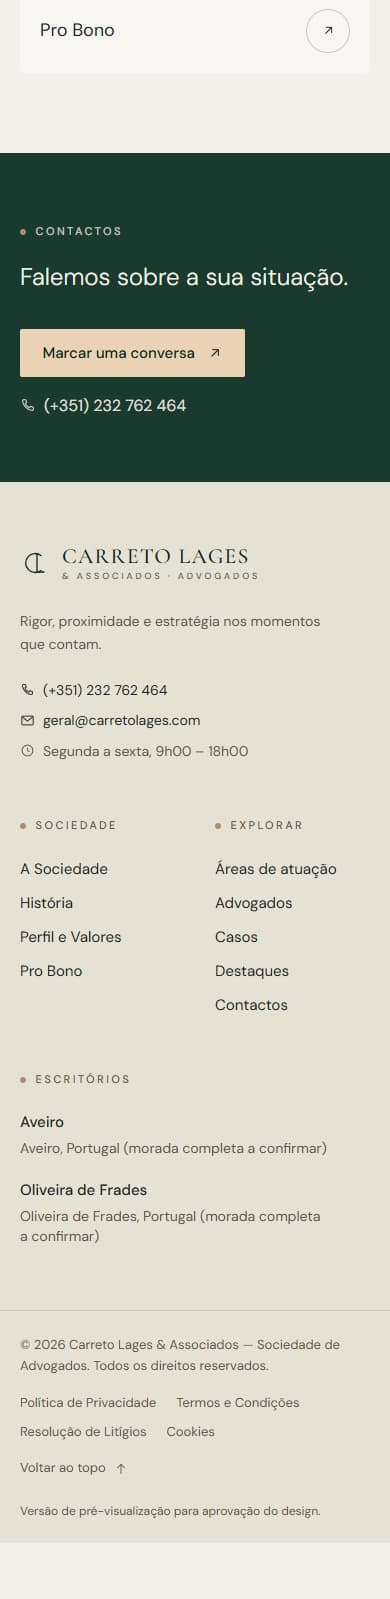
\includegraphics[width=0.235\textwidth]{screenshots/mobile/pt/sociedade-2.jpg}\par\medskip
\bigskip
\needspace{8\baselineskip}
\subsection*{Mais de duas décadas ao lado dos nossos clientes.}
\addcontentsline{toc}{subsection}{Mais de duas décadas ao lado dos nossos clientes. (\texttt{/sociedade/historia})}
\noindent{\small\color{tintasuave}\texttt{/sociedade/historia}}\par\smallskip
\noindent{\footnotesize Computador (1440\,px)}\par\smallskip
\noindent 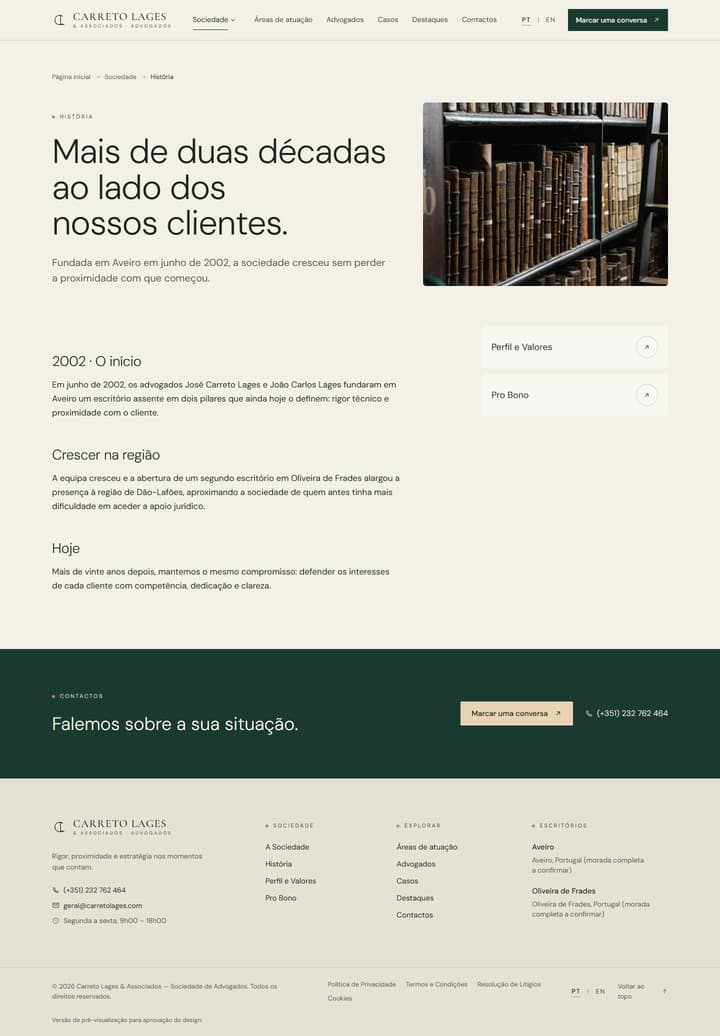
\includegraphics[width=0.485\textwidth]{screenshots/desktop/pt/sociedade--historia.jpg}\par\medskip
\noindent{\footnotesize Telemóvel (390\,px)}\par\smallskip
\noindent 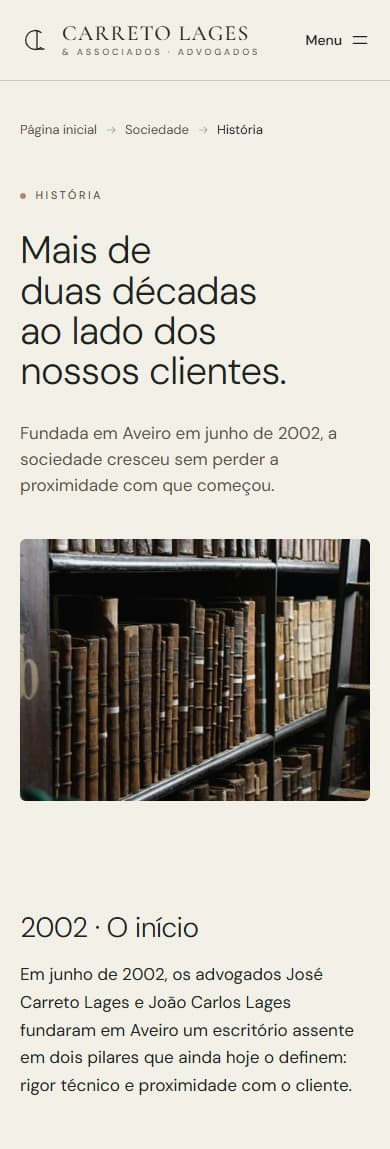
\includegraphics[width=0.235\textwidth]{screenshots/mobile/pt/sociedade--historia-1.jpg}\hspace{0.012\textwidth}
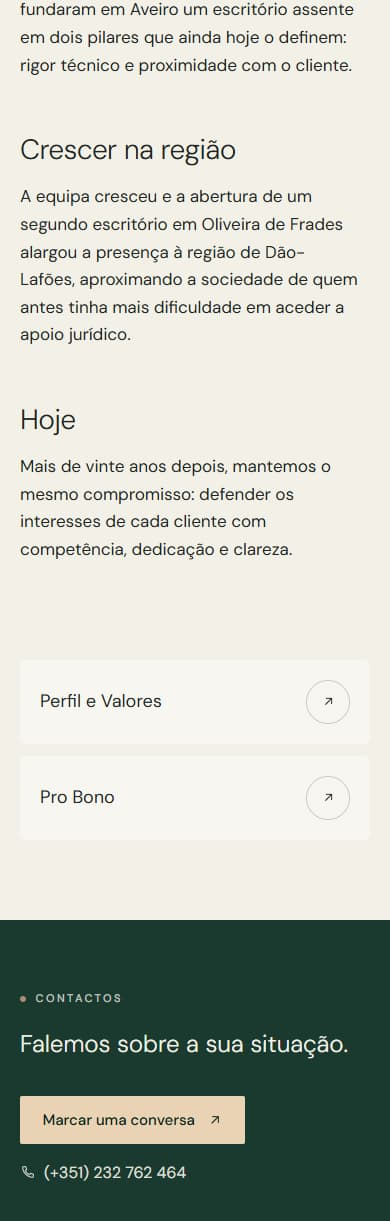
\includegraphics[width=0.235\textwidth]{screenshots/mobile/pt/sociedade--historia-2.jpg}\hspace{0.012\textwidth}
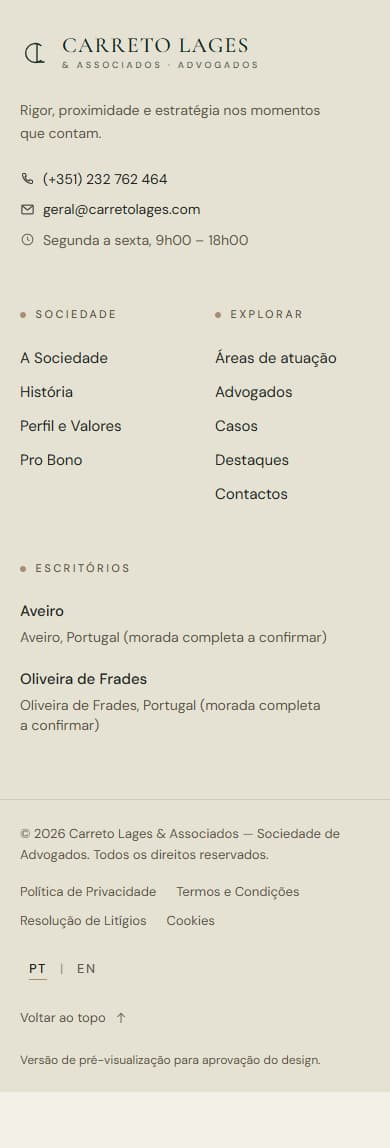
\includegraphics[width=0.235\textwidth]{screenshots/mobile/pt/sociedade--historia-3.jpg}\par\medskip
\bigskip
\needspace{8\baselineskip}
\subsection*{Os princípios por detrás de cada decisão.}
\addcontentsline{toc}{subsection}{Os princípios por detrás de cada decisão. (\texttt{/sociedade/perfil-e-valores})}
\noindent{\small\color{tintasuave}\texttt{/sociedade/perfil-e-valores}}\par\smallskip
\noindent{\footnotesize Computador (1440\,px)}\par\smallskip
\noindent 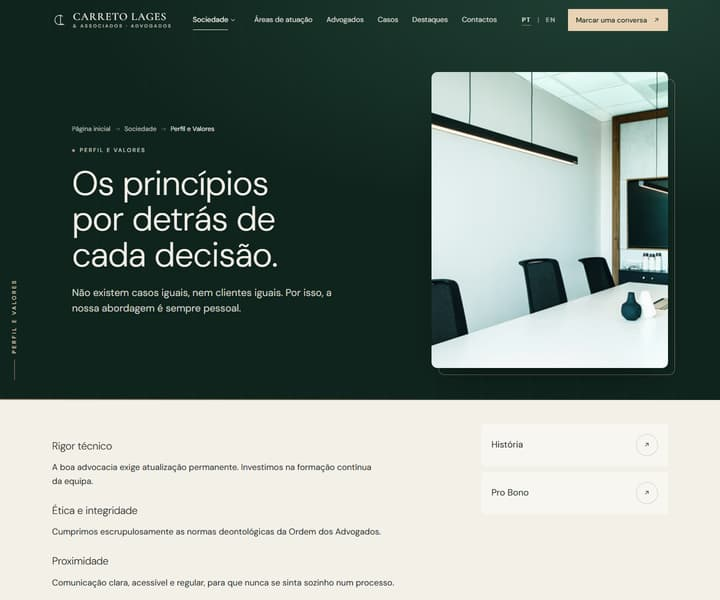
\includegraphics[width=0.485\textwidth]{screenshots/desktop/pt/sociedade--perfil-e-valores-1.jpg}\hspace{0.012\textwidth}
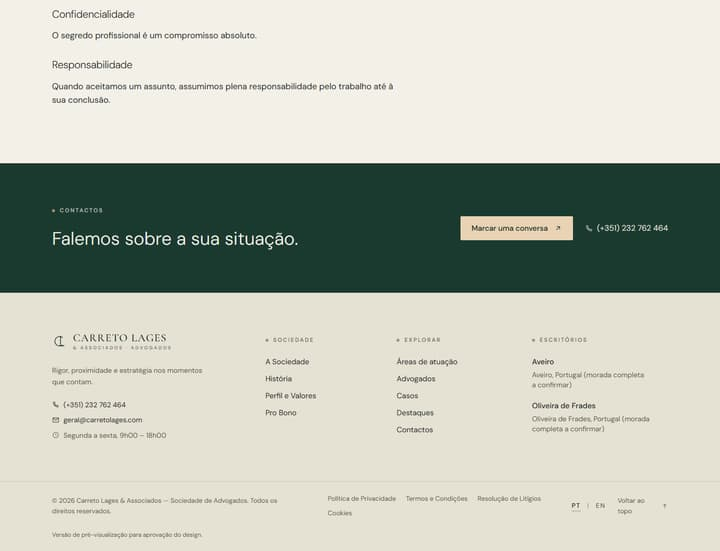
\includegraphics[width=0.485\textwidth]{screenshots/desktop/pt/sociedade--perfil-e-valores-2.jpg}\par\medskip
\noindent{\footnotesize Telemóvel (390\,px)}\par\smallskip
\noindent 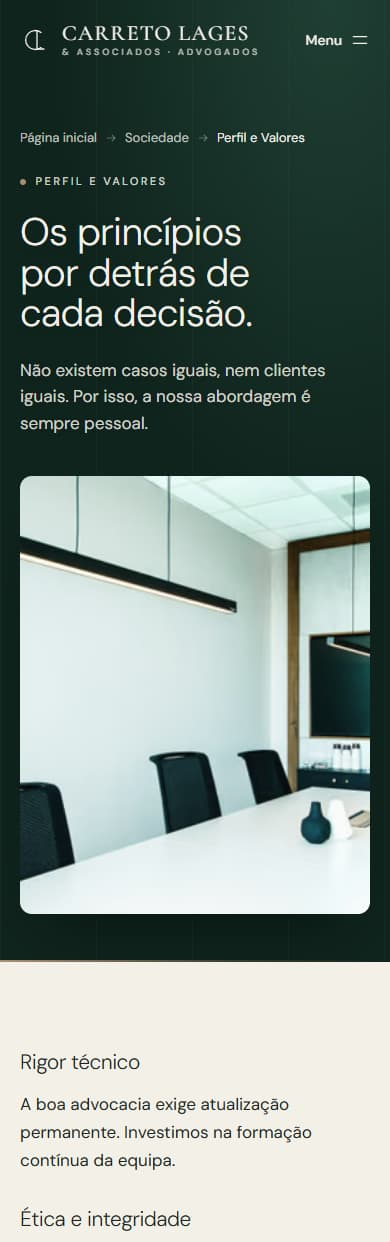
\includegraphics[width=0.235\textwidth]{screenshots/mobile/pt/sociedade--perfil-e-valores-1.jpg}\hspace{0.012\textwidth}
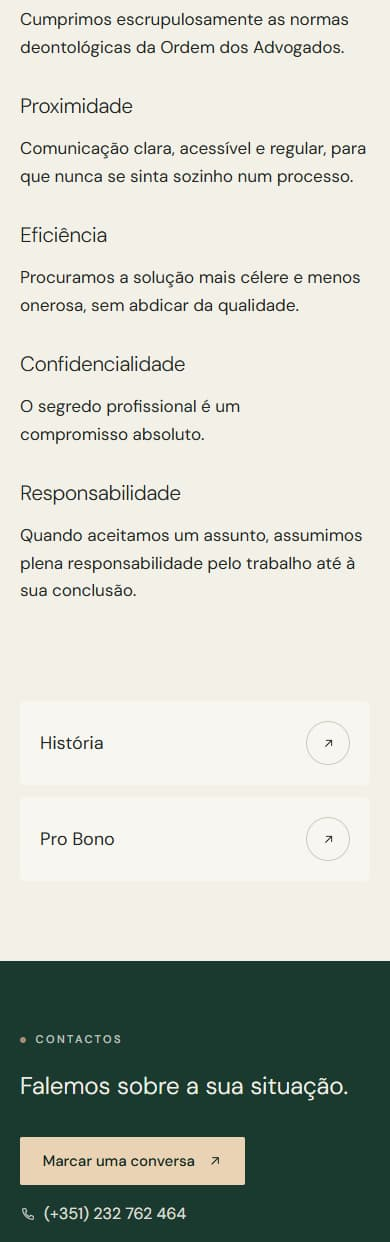
\includegraphics[width=0.235\textwidth]{screenshots/mobile/pt/sociedade--perfil-e-valores-2.jpg}\hspace{0.012\textwidth}
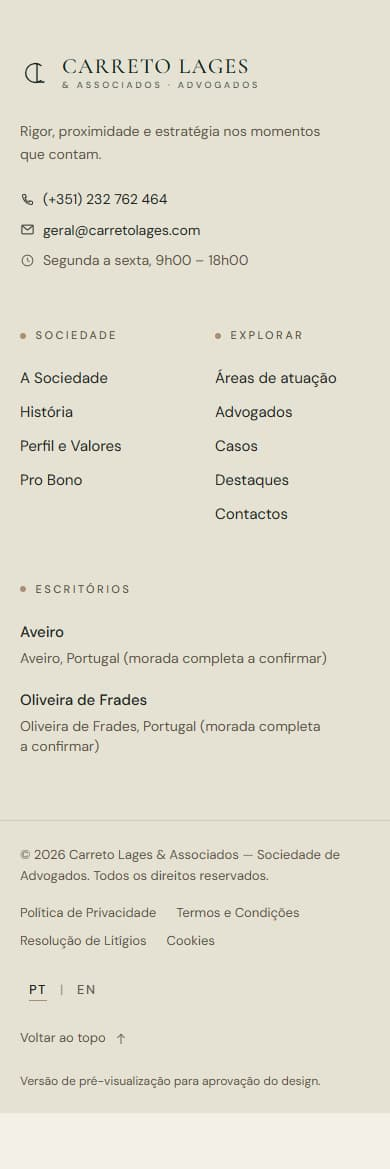
\includegraphics[width=0.235\textwidth]{screenshots/mobile/pt/sociedade--perfil-e-valores-3.jpg}\par\medskip
\bigskip
\needspace{8\baselineskip}
\subsection*{O acesso à justiça é um direito.}
\addcontentsline{toc}{subsection}{O acesso à justiça é um direito. (\texttt{/sociedade/pro-bono})}
\noindent{\small\color{tintasuave}\texttt{/sociedade/pro-bono}}\par\smallskip
\noindent{\footnotesize Computador (1440\,px)}\par\smallskip
\noindent 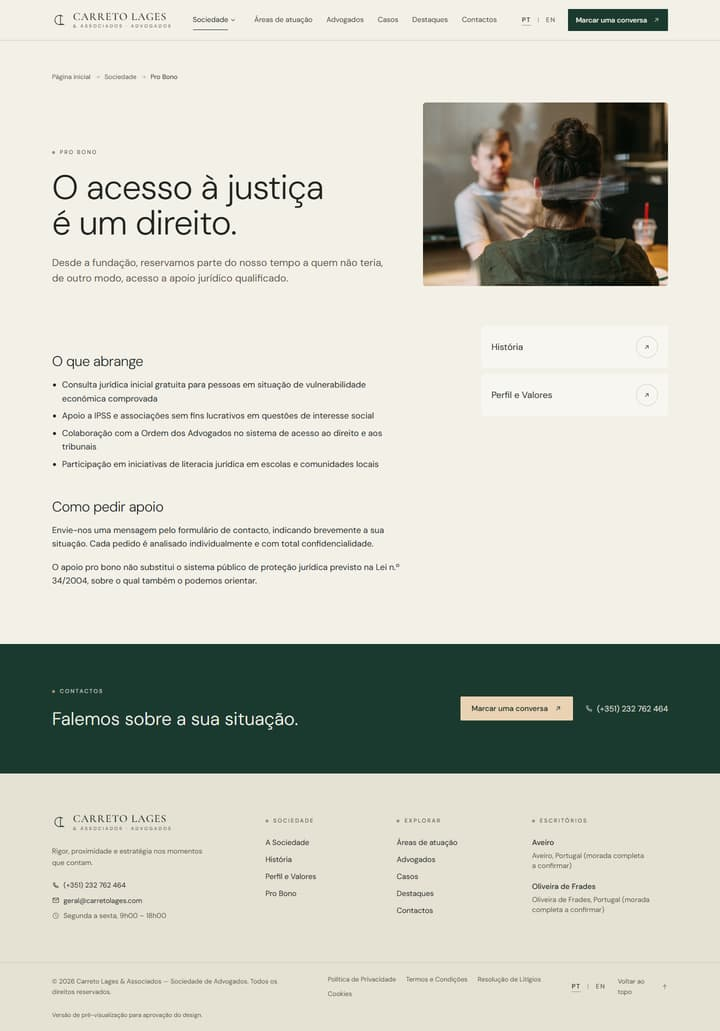
\includegraphics[width=0.485\textwidth]{screenshots/desktop/pt/sociedade--pro-bono.jpg}\par\medskip
\noindent{\footnotesize Telemóvel (390\,px)}\par\smallskip
\noindent 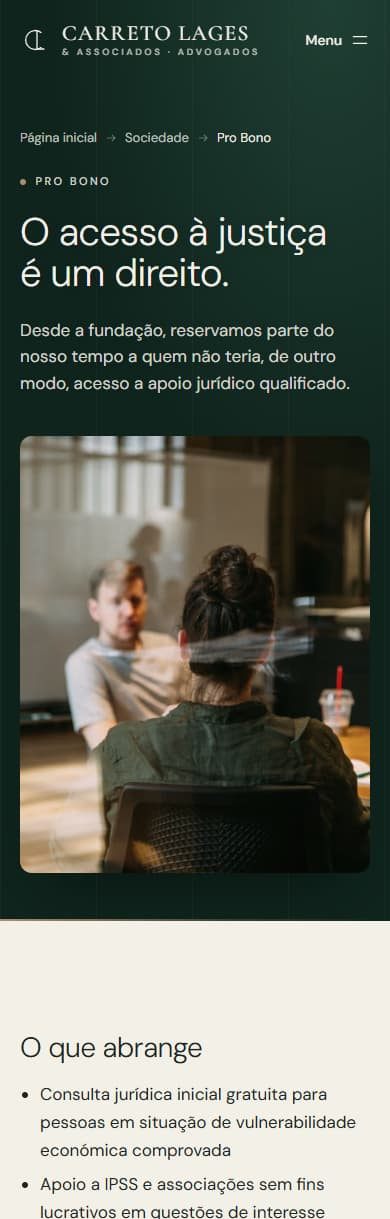
\includegraphics[width=0.235\textwidth]{screenshots/mobile/pt/sociedade--pro-bono-1.jpg}\hspace{0.012\textwidth}
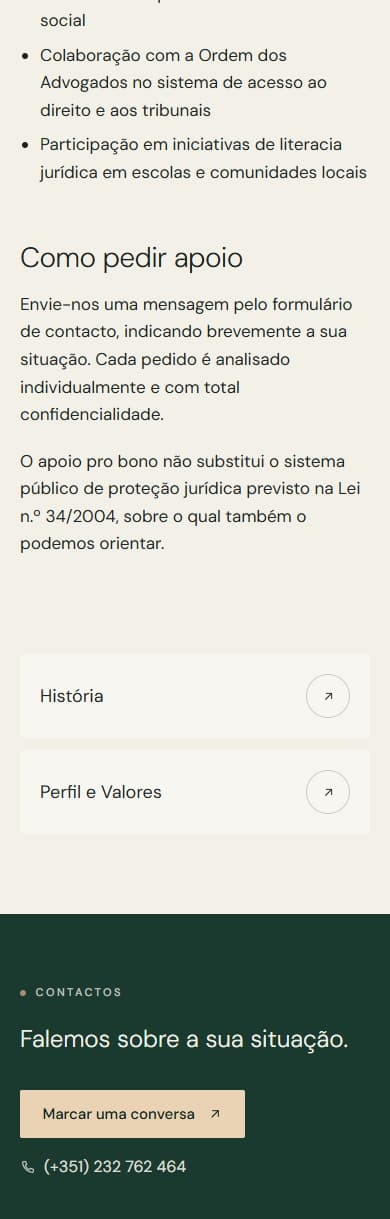
\includegraphics[width=0.235\textwidth]{screenshots/mobile/pt/sociedade--pro-bono-2.jpg}\hspace{0.012\textwidth}
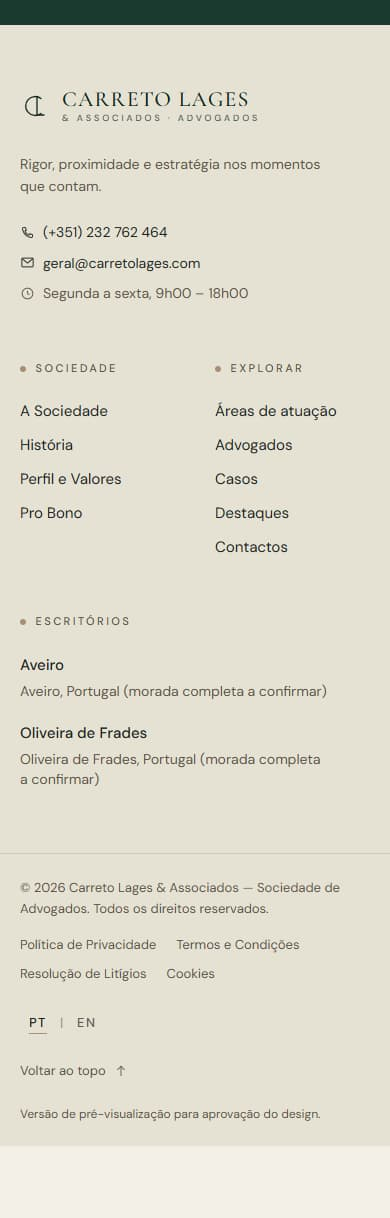
\includegraphics[width=0.235\textwidth]{screenshots/mobile/pt/sociedade--pro-bono-3.jpg}\par\medskip
\bigskip
\needspace{8\baselineskip}
\subsection*{Termos e Condições}
\addcontentsline{toc}{subsection}{Termos e Condições (\texttt{/termos-e-condicoes})}
\noindent{\small\color{tintasuave}\texttt{/termos-e-condicoes}}\par\smallskip
\noindent{\footnotesize Computador (1440\,px)}\par\smallskip
\noindent 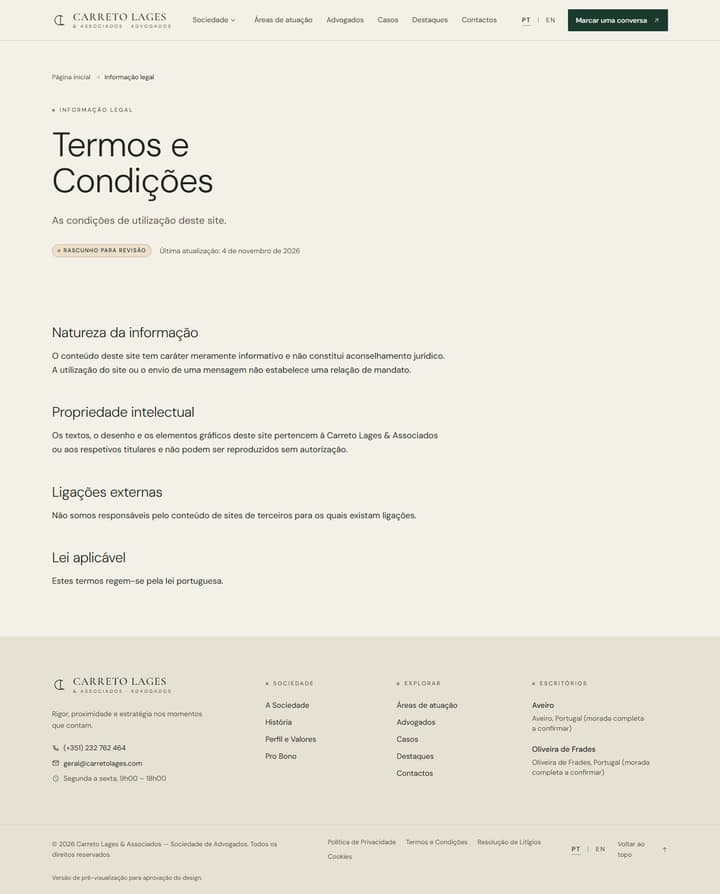
\includegraphics[width=0.485\textwidth]{screenshots/desktop/pt/termos-e-condicoes.jpg}\par\medskip
\noindent{\footnotesize Telemóvel (390\,px)}\par\smallskip
\noindent 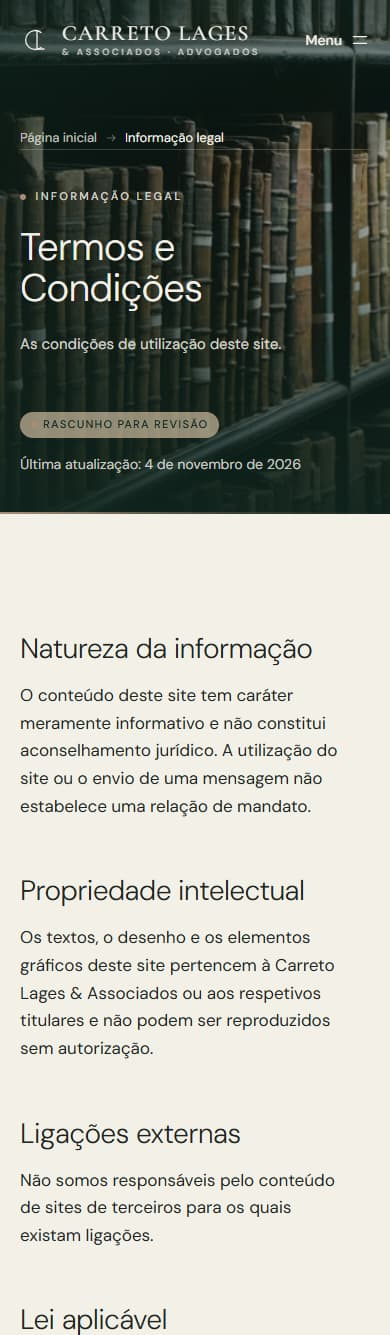
\includegraphics[width=0.235\textwidth]{screenshots/mobile/pt/termos-e-condicoes-1.jpg}\hspace{0.012\textwidth}
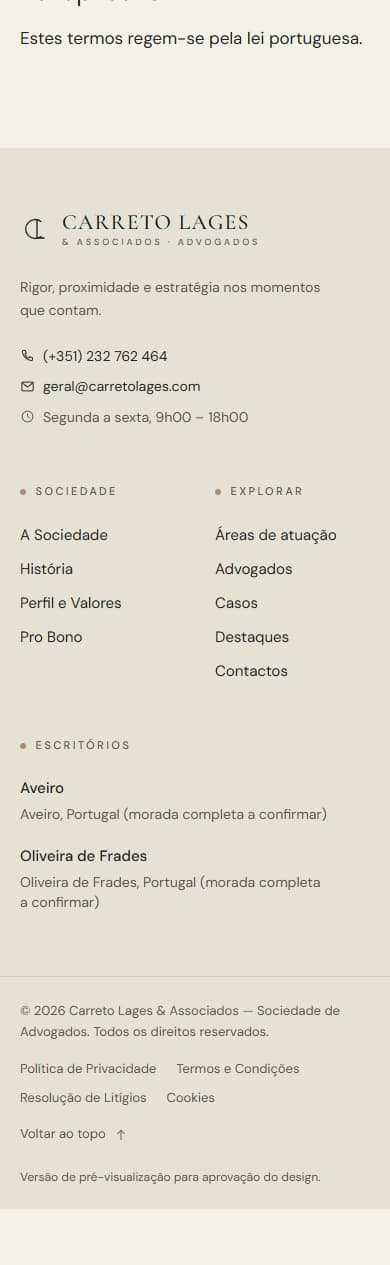
\includegraphics[width=0.235\textwidth]{screenshots/mobile/pt/termos-e-condicoes-2.jpg}\par\medskip
\bigskip
\clearpage
\section{Páginas — versão inglesa}
\needspace{8\baselineskip}
\subsection*{Important decisions. In safe hands.}
\addcontentsline{toc}{subsection}{Important decisions. In safe hands. (\texttt{/en})}
\noindent{\small\color{tintasuave}\texttt{/en}}\par\smallskip
\noindent{\footnotesize Computador (1440\,px)}\par\smallskip
\noindent 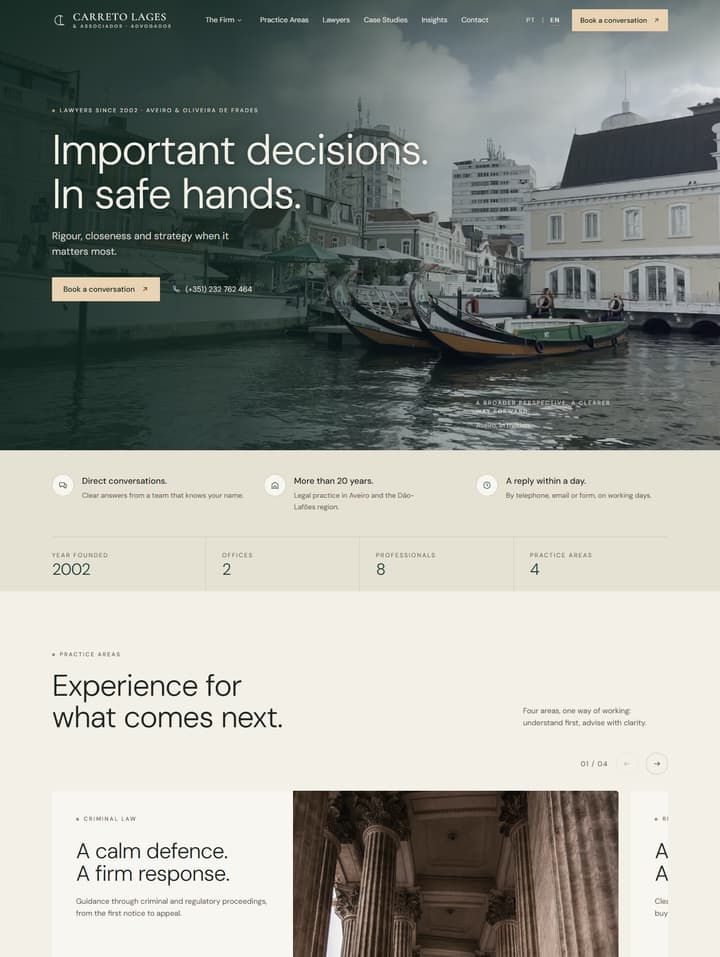
\includegraphics[width=0.485\textwidth]{screenshots/desktop/en/home-1.jpg}\hspace{0.012\textwidth}
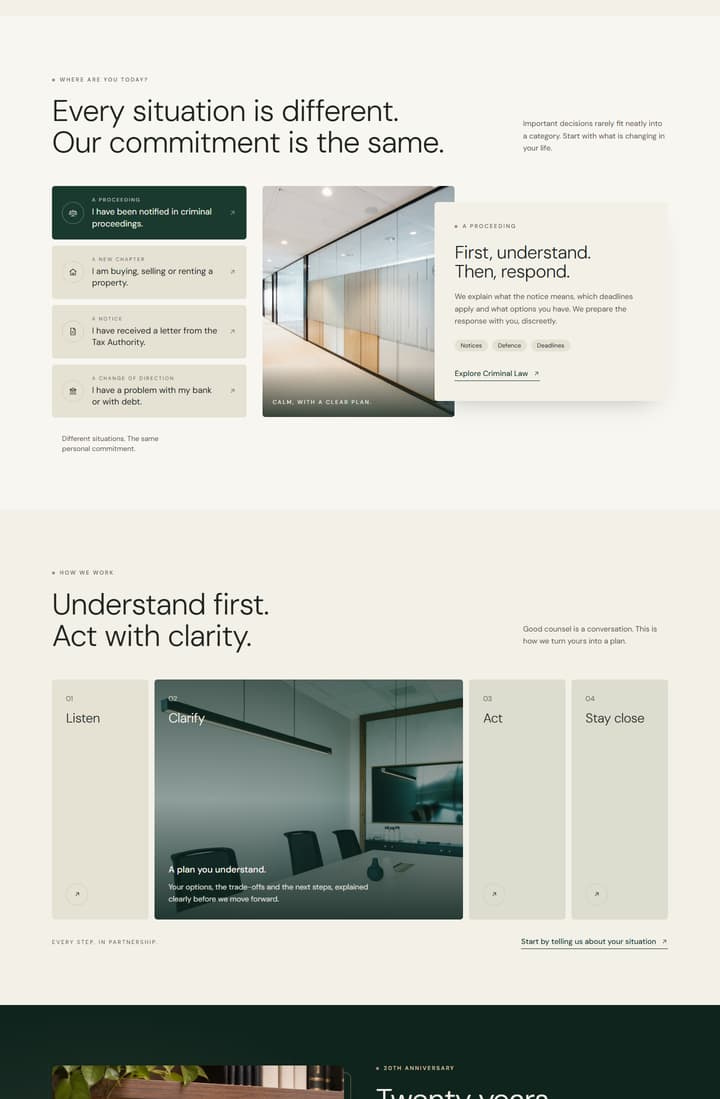
\includegraphics[width=0.485\textwidth]{screenshots/desktop/en/home-2.jpg}\par\medskip
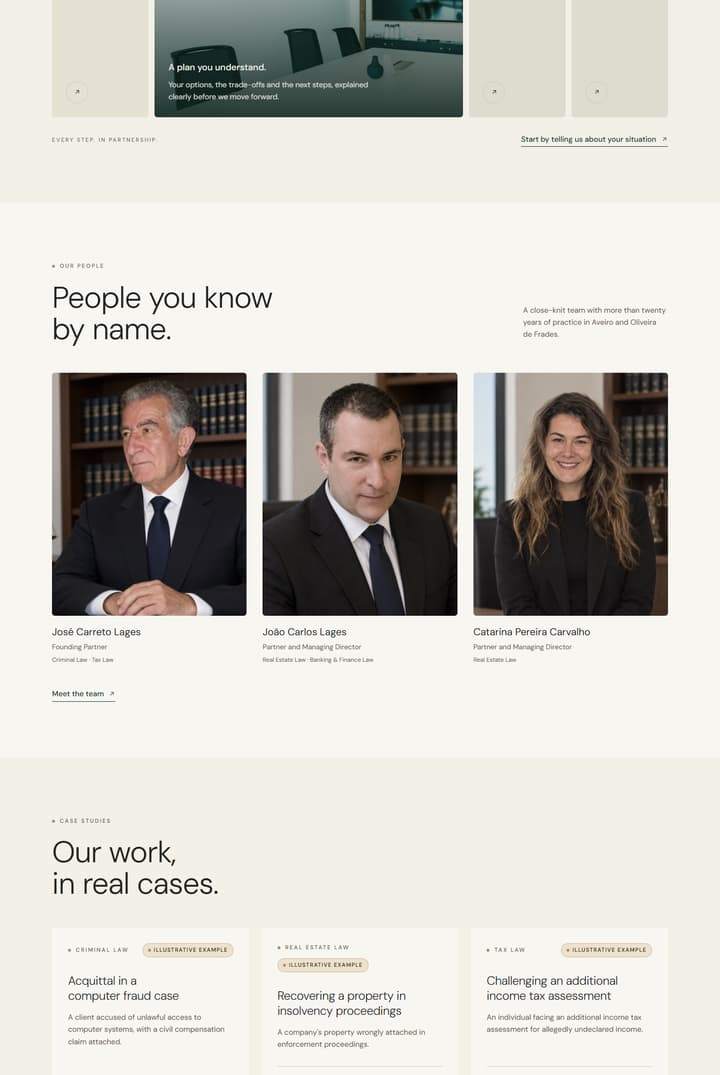
\includegraphics[width=0.485\textwidth]{screenshots/desktop/en/home-3.jpg}\hspace{0.012\textwidth}
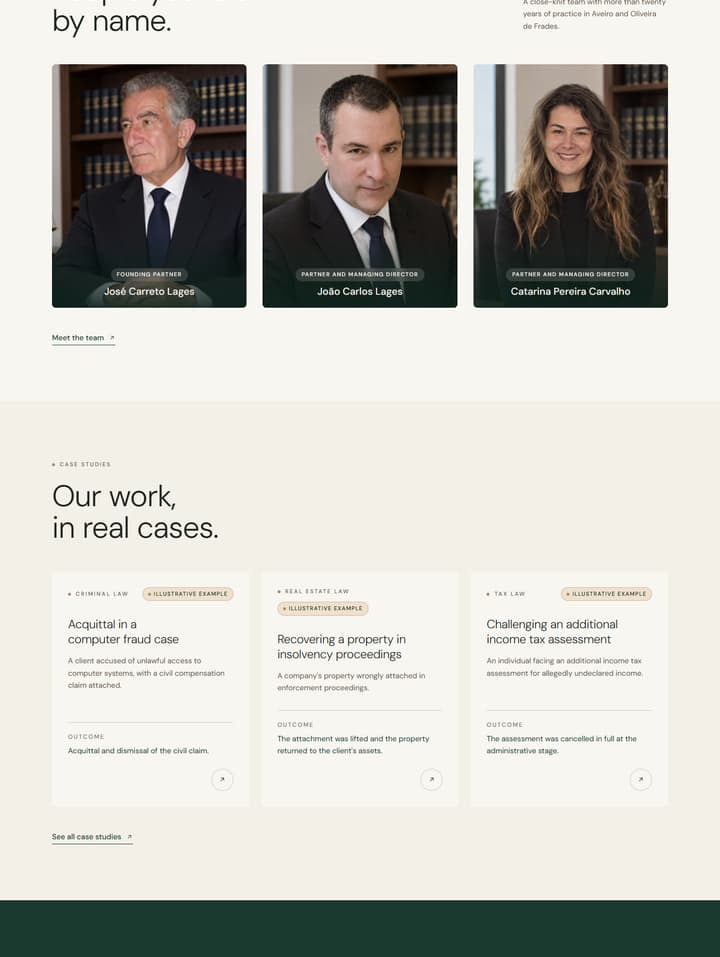
\includegraphics[width=0.485\textwidth]{screenshots/desktop/en/home-4.jpg}\par\medskip
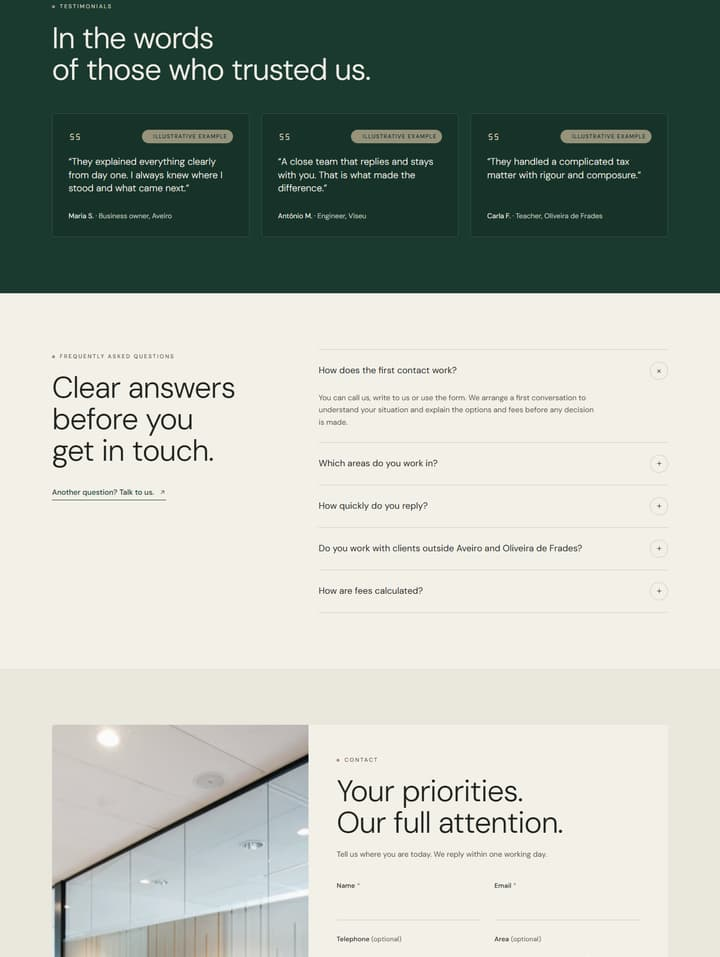
\includegraphics[width=0.485\textwidth]{screenshots/desktop/en/home-5.jpg}\par\medskip
\noindent{\footnotesize Telemóvel (390\,px)}\par\smallskip
\noindent 
\includegraphics[width=0.235\textwidth]{screenshots/mobile/en/home-1.jpg}\hspace{0.012\textwidth}
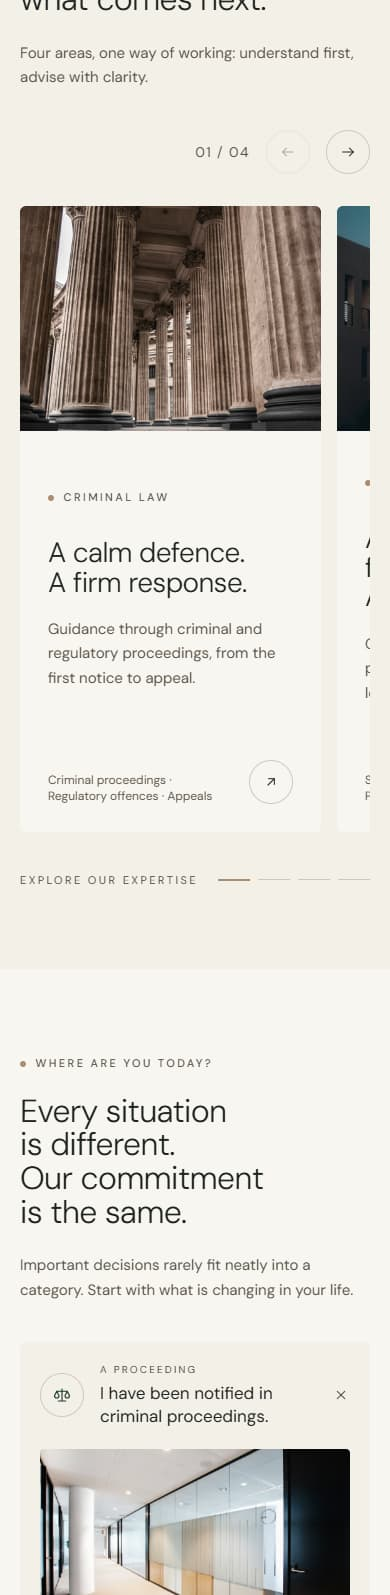
\includegraphics[width=0.235\textwidth]{screenshots/mobile/en/home-2.jpg}\hspace{0.012\textwidth}
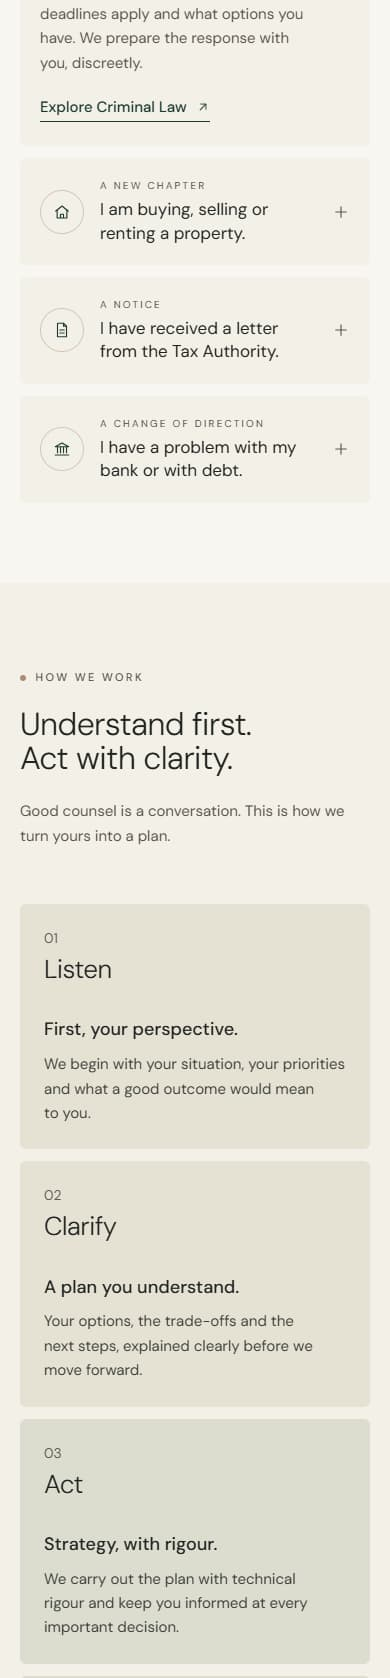
\includegraphics[width=0.235\textwidth]{screenshots/mobile/en/home-3.jpg}\hspace{0.012\textwidth}
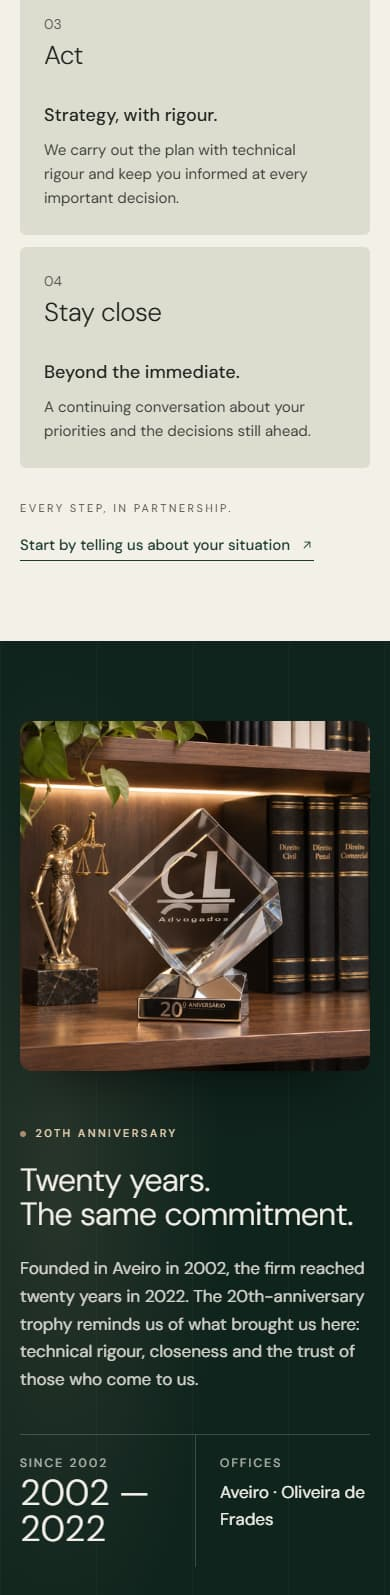
\includegraphics[width=0.235\textwidth]{screenshots/mobile/en/home-4.jpg}\par\medskip
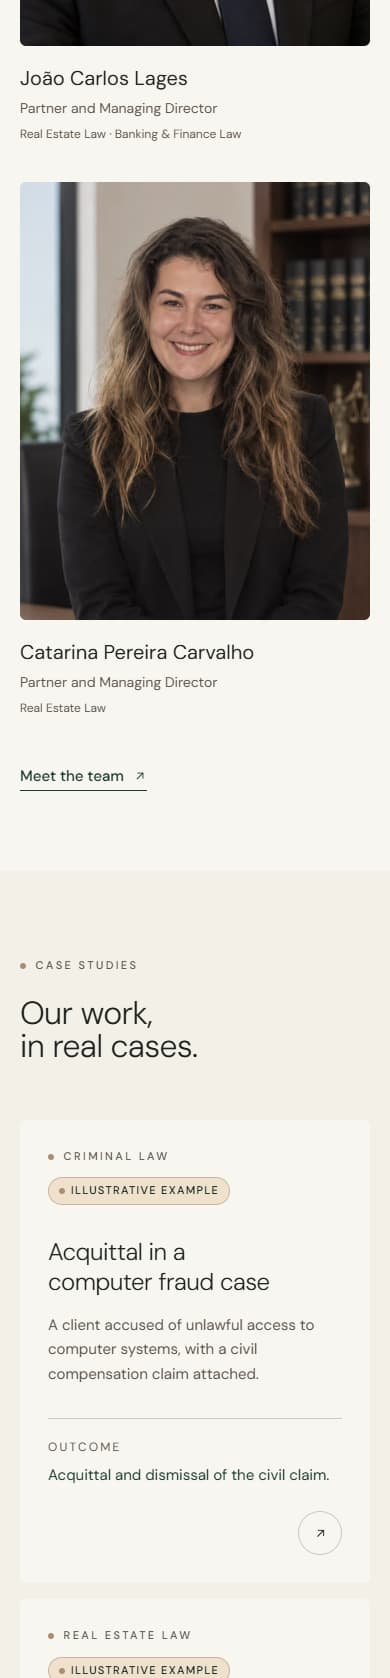
\includegraphics[width=0.235\textwidth]{screenshots/mobile/en/home-5.jpg}\hspace{0.012\textwidth}
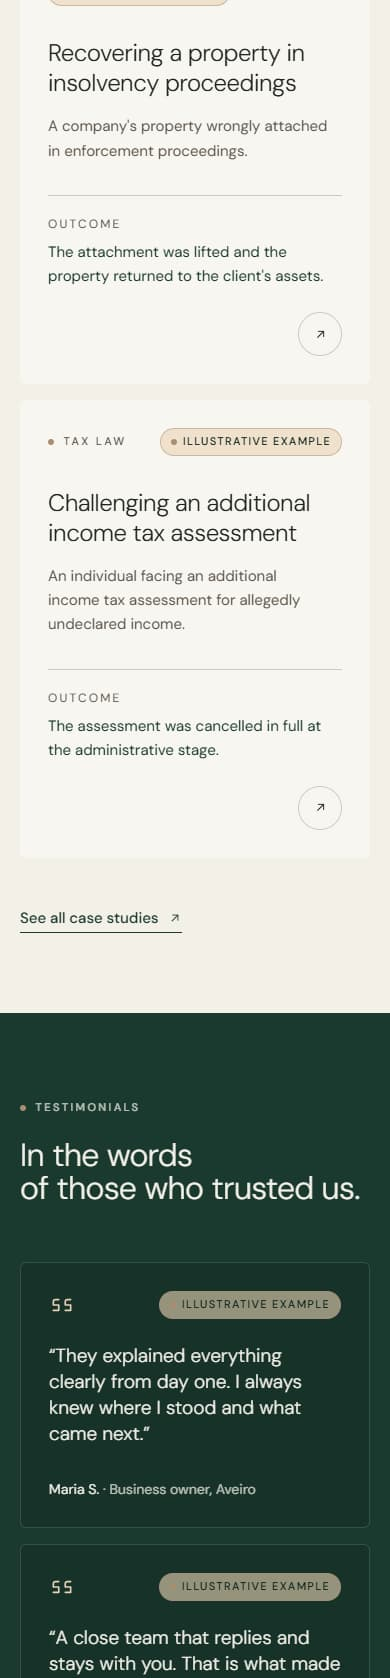
\includegraphics[width=0.235\textwidth]{screenshots/mobile/en/home-6.jpg}\hspace{0.012\textwidth}
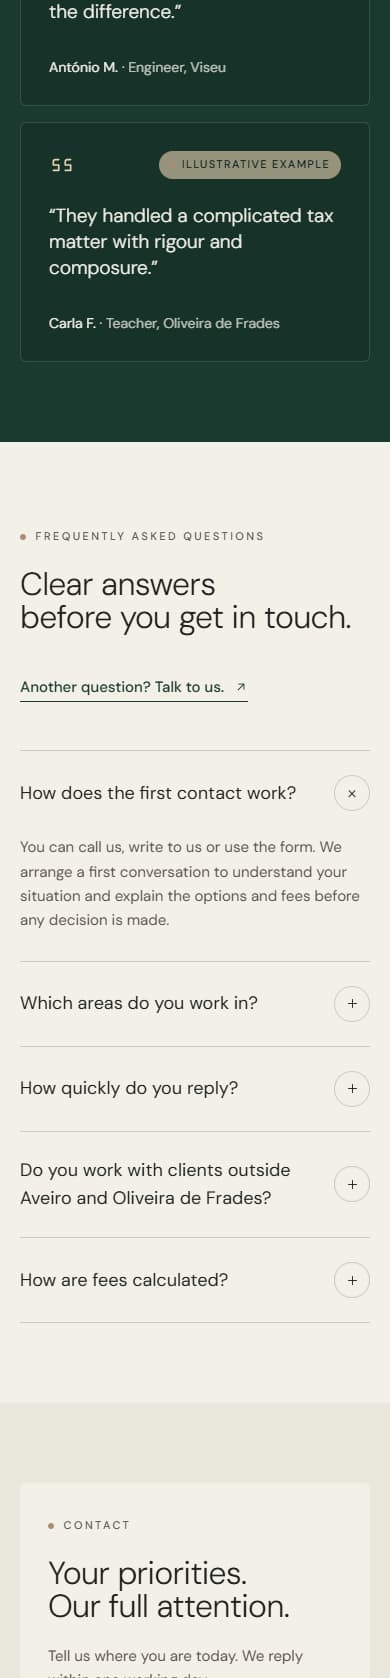
\includegraphics[width=0.235\textwidth]{screenshots/mobile/en/home-7.jpg}\hspace{0.012\textwidth}
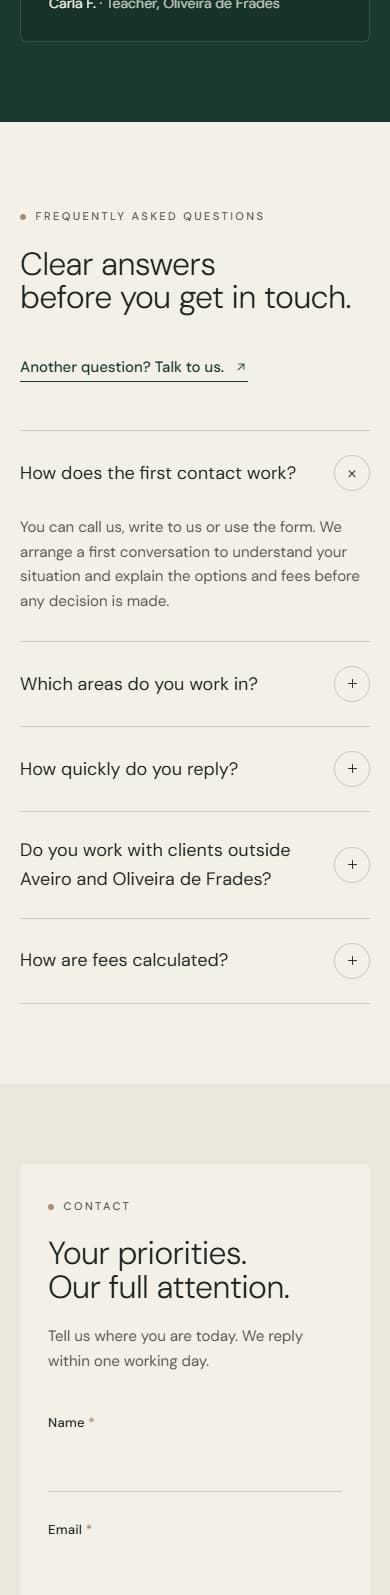
\includegraphics[width=0.235\textwidth]{screenshots/mobile/en/home-8.jpg}\par\medskip
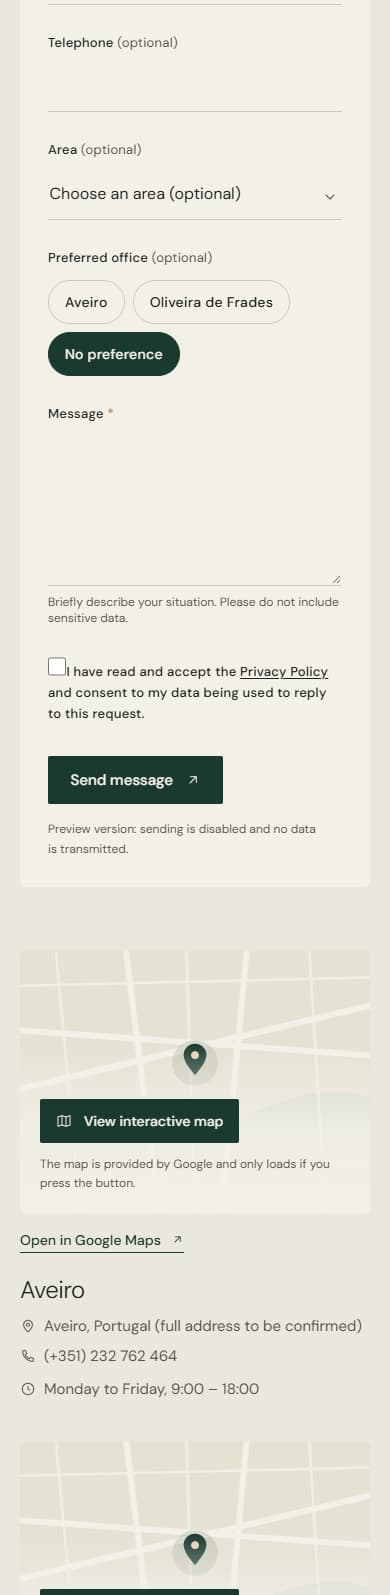
\includegraphics[width=0.235\textwidth]{screenshots/mobile/en/home-9.jpg}\par\medskip
\bigskip
\needspace{8\baselineskip}
\subsection*{This page does not exist.}
\addcontentsline{toc}{subsection}{This page does not exist. (\texttt{/en/404})}
\noindent{\small\color{tintasuave}\texttt{/en/404}}\par\smallskip
\noindent{\footnotesize Computador (1440\,px)}\par\smallskip
\noindent 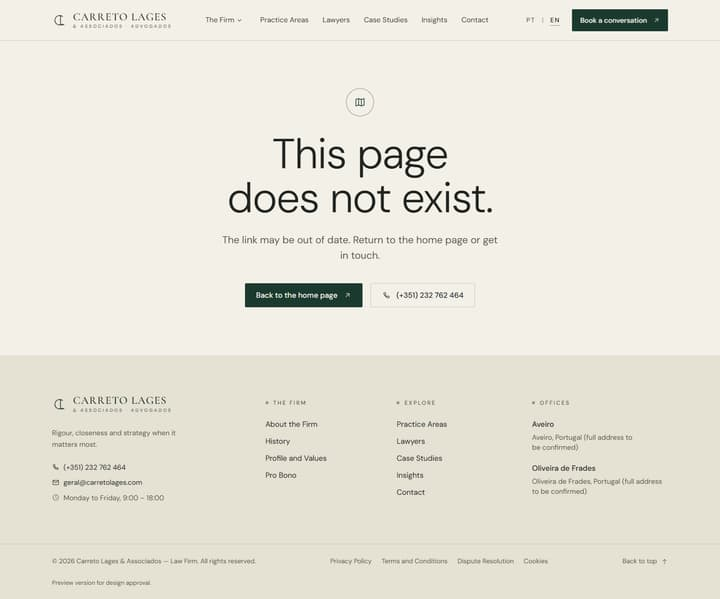
\includegraphics[width=0.485\textwidth]{screenshots/desktop/en/404.jpg}\par\medskip
\noindent{\footnotesize Telemóvel (390\,px)}\par\smallskip
\noindent 
\includegraphics[width=0.235\textwidth]{screenshots/mobile/en/404-1.jpg}\hspace{0.012\textwidth}
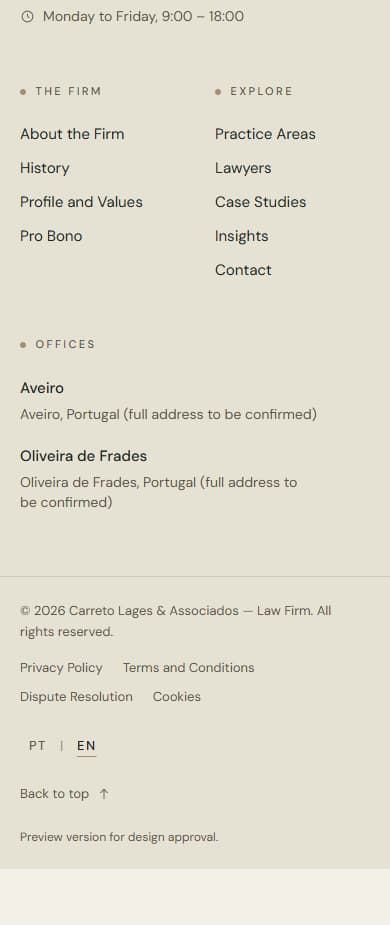
\includegraphics[width=0.235\textwidth]{screenshots/mobile/en/404-2.jpg}\par\medskip
\bigskip
\needspace{8\baselineskip}
\subsection*{Our work, in real cases.}
\addcontentsline{toc}{subsection}{Our work, in real cases. (\texttt{/en/case-studies})}
\noindent{\small\color{tintasuave}\texttt{/en/case-studies}}\par\smallskip
\noindent{\footnotesize Computador (1440\,px)}\par\smallskip
\noindent 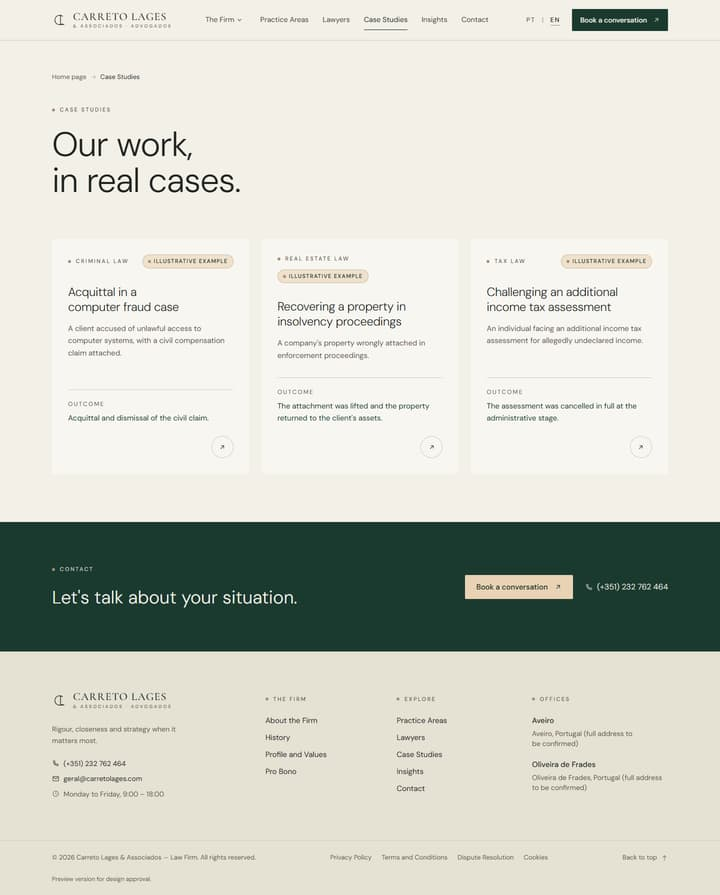
\includegraphics[width=0.485\textwidth]{screenshots/desktop/en/case-studies.jpg}\par\medskip
\noindent{\footnotesize Telemóvel (390\,px)}\par\smallskip
\noindent 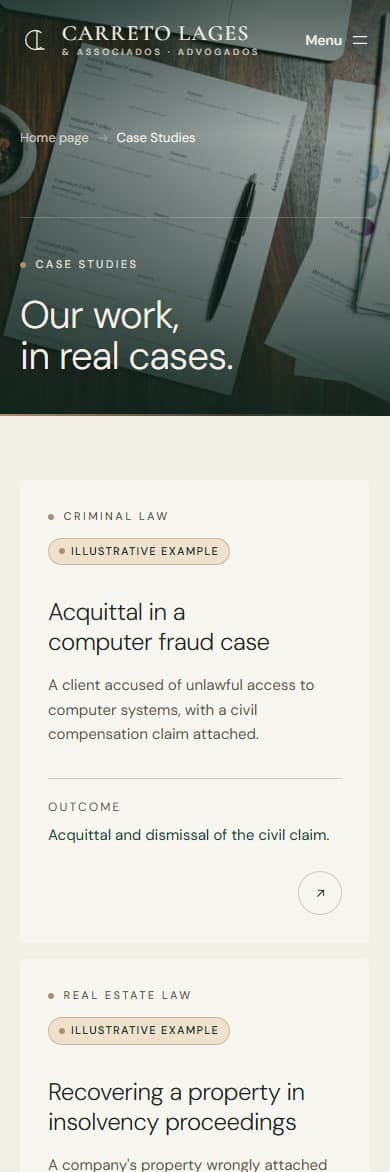
\includegraphics[width=0.235\textwidth]{screenshots/mobile/en/case-studies-1.jpg}\hspace{0.012\textwidth}
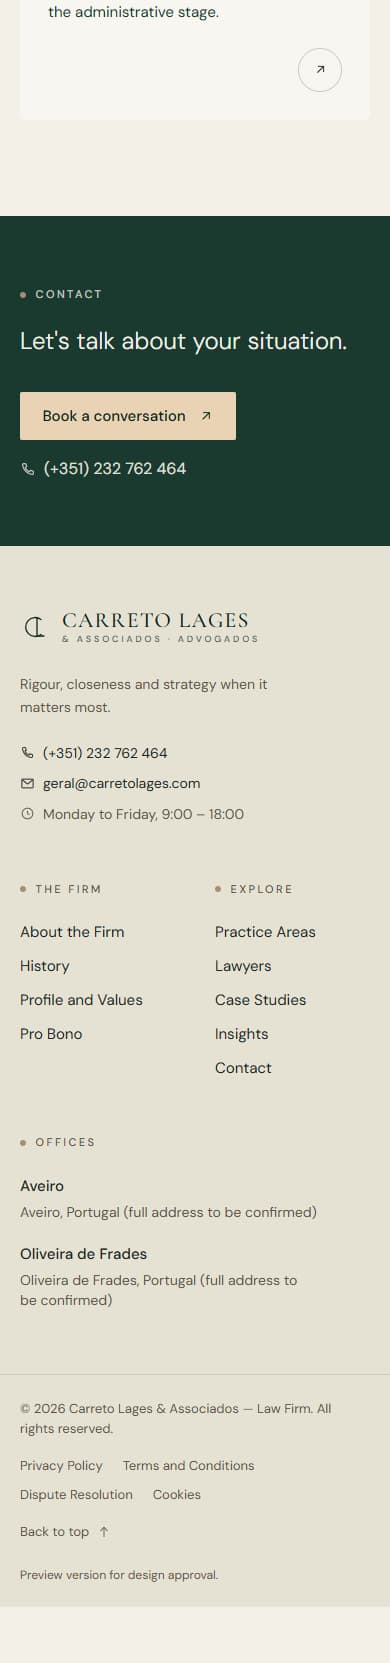
\includegraphics[width=0.235\textwidth]{screenshots/mobile/en/case-studies-2.jpg}\par\medskip
\bigskip
\needspace{8\baselineskip}
\subsection*{Acquittal in a computer fraud case}
\addcontentsline{toc}{subsection}{Acquittal in a computer fraud case (\texttt{/en/case-studies/acquittal-computer-fraud})}
\noindent{\small\color{tintasuave}\texttt{/en/case-studies/acquittal-computer-fraud}}\par\smallskip
\noindent{\footnotesize Computador (1440\,px)}\par\smallskip
\noindent 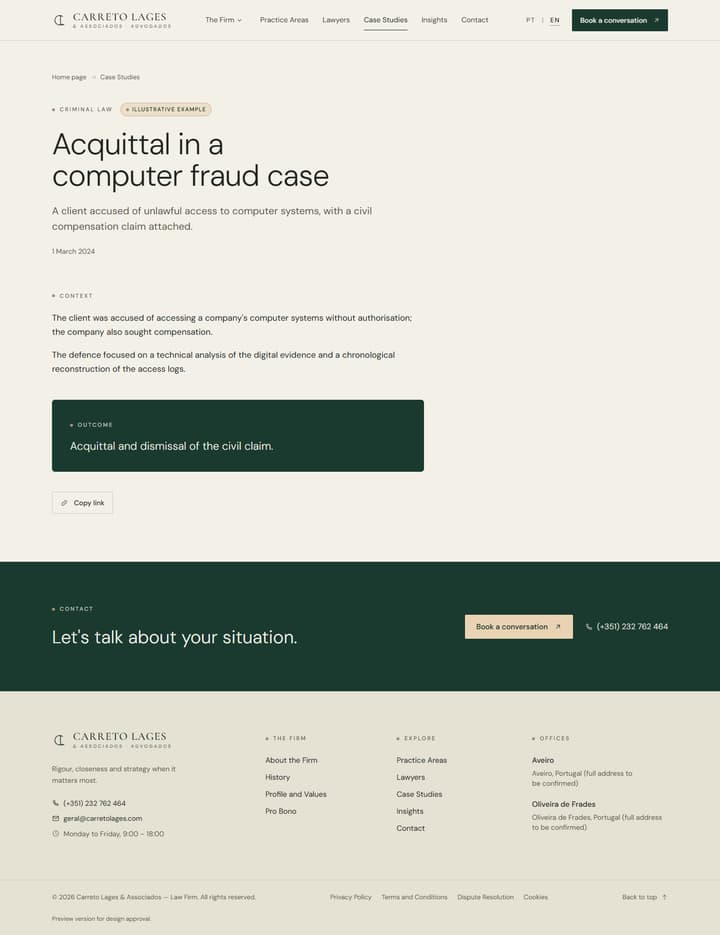
\includegraphics[width=0.485\textwidth]{screenshots/desktop/en/case-studies--acquittal-computer-fraud.jpg}\par\medskip
\noindent{\footnotesize Telemóvel (390\,px)}\par\smallskip
\noindent 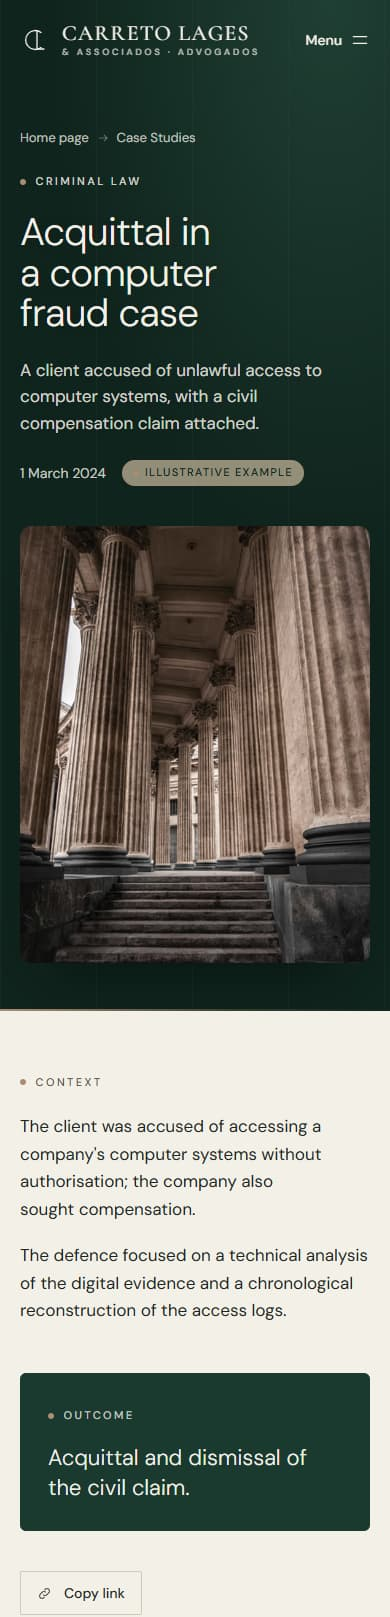
\includegraphics[width=0.235\textwidth]{screenshots/mobile/en/case-studies--acquittal-computer-fraud-1.jpg}\hspace{0.012\textwidth}
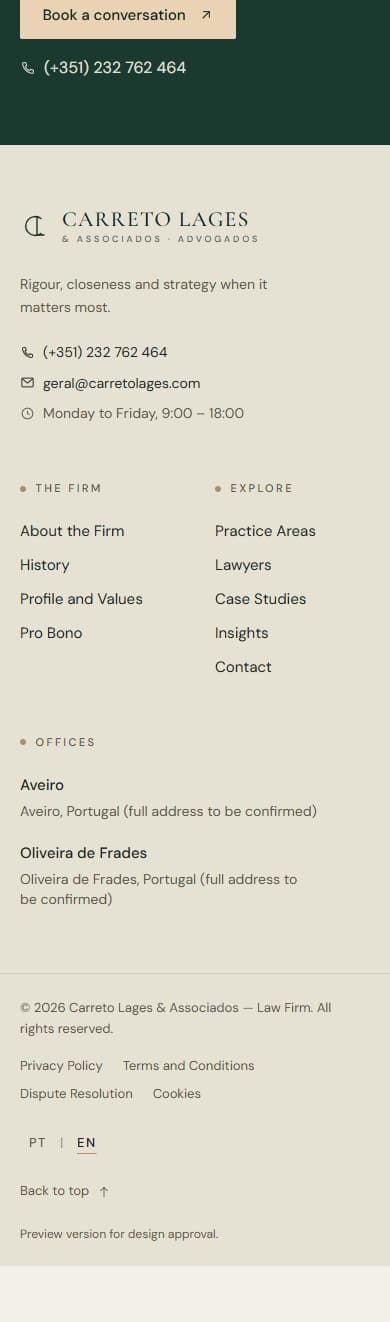
\includegraphics[width=0.235\textwidth]{screenshots/mobile/en/case-studies--acquittal-computer-fraud-2.jpg}\par\medskip
\bigskip
\needspace{8\baselineskip}
\subsection*{Challenging an additional income tax assessment}
\addcontentsline{toc}{subsection}{Challenging an additional income tax assessment (\texttt{/en/case-studies/income-tax-assessment-appeal})}
\noindent{\small\color{tintasuave}\texttt{/en/case-studies/income-tax-assessment-appeal}}\par\smallskip
\noindent{\footnotesize Computador (1440\,px)}\par\smallskip
\noindent 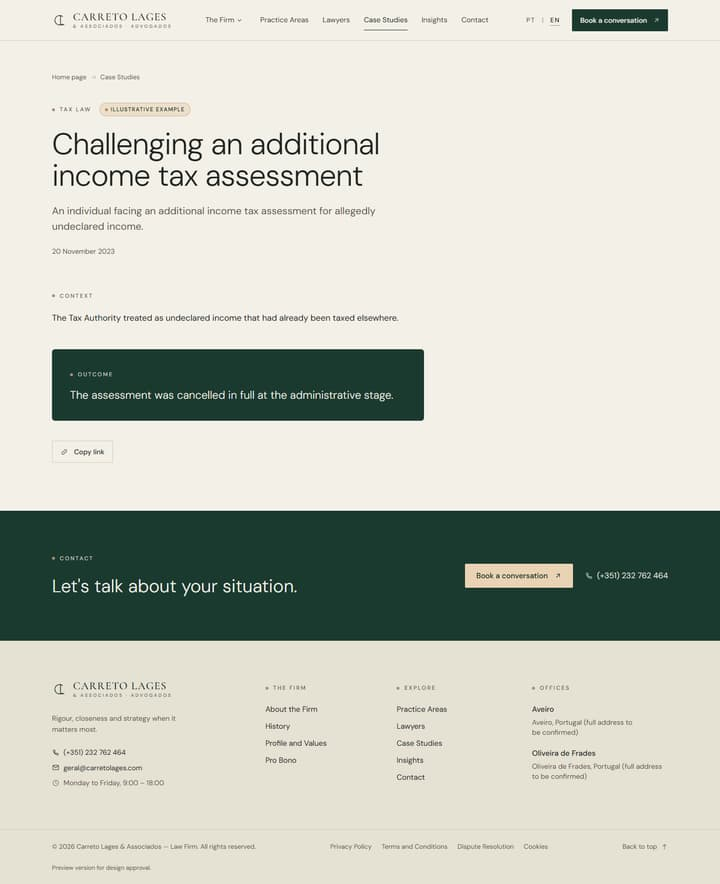
\includegraphics[width=0.485\textwidth]{screenshots/desktop/en/case-studies--income-tax-assessment-appeal.jpg}\par\medskip
\noindent{\footnotesize Telemóvel (390\,px)}\par\smallskip
\noindent 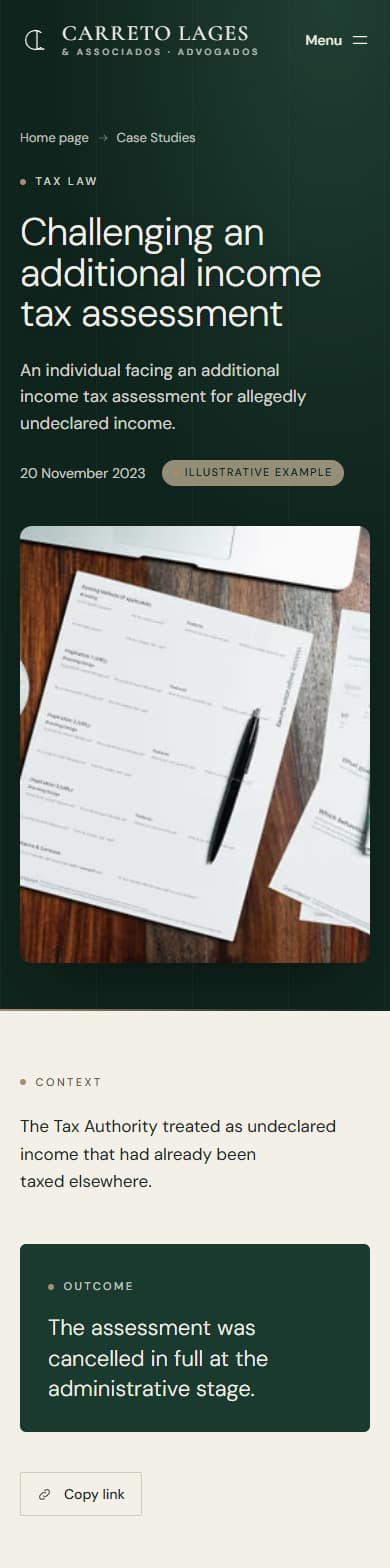
\includegraphics[width=0.235\textwidth]{screenshots/mobile/en/case-studies--income-tax-assessment-appeal-1.jpg}\hspace{0.012\textwidth}
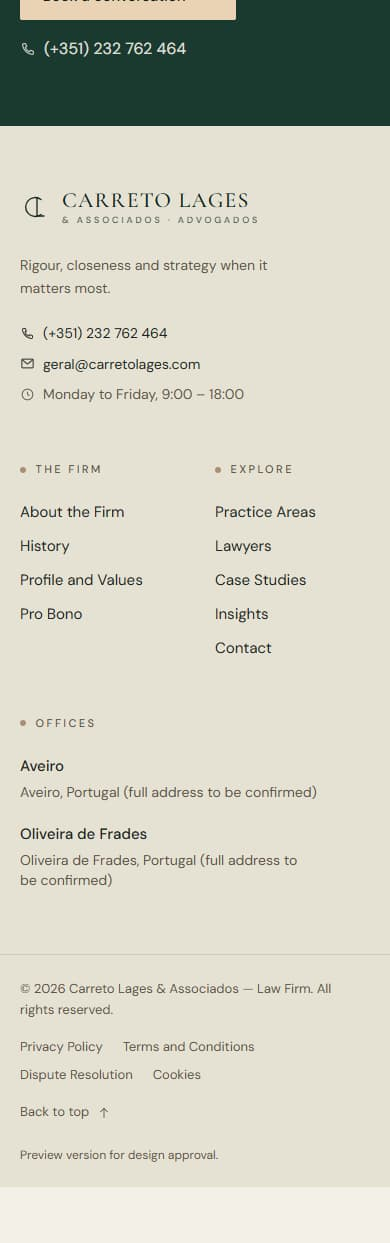
\includegraphics[width=0.235\textwidth]{screenshots/mobile/en/case-studies--income-tax-assessment-appeal-2.jpg}\par\medskip
\bigskip
\needspace{8\baselineskip}
\subsection*{Recovering a property in insolvency proceedings}
\addcontentsline{toc}{subsection}{Recovering a property in insolvency proceedings (\texttt{/en/case-studies/property-recovered-insolvency})}
\noindent{\small\color{tintasuave}\texttt{/en/case-studies/property-recovered-insolvency}}\par\smallskip
\noindent{\footnotesize Computador (1440\,px)}\par\smallskip
\noindent 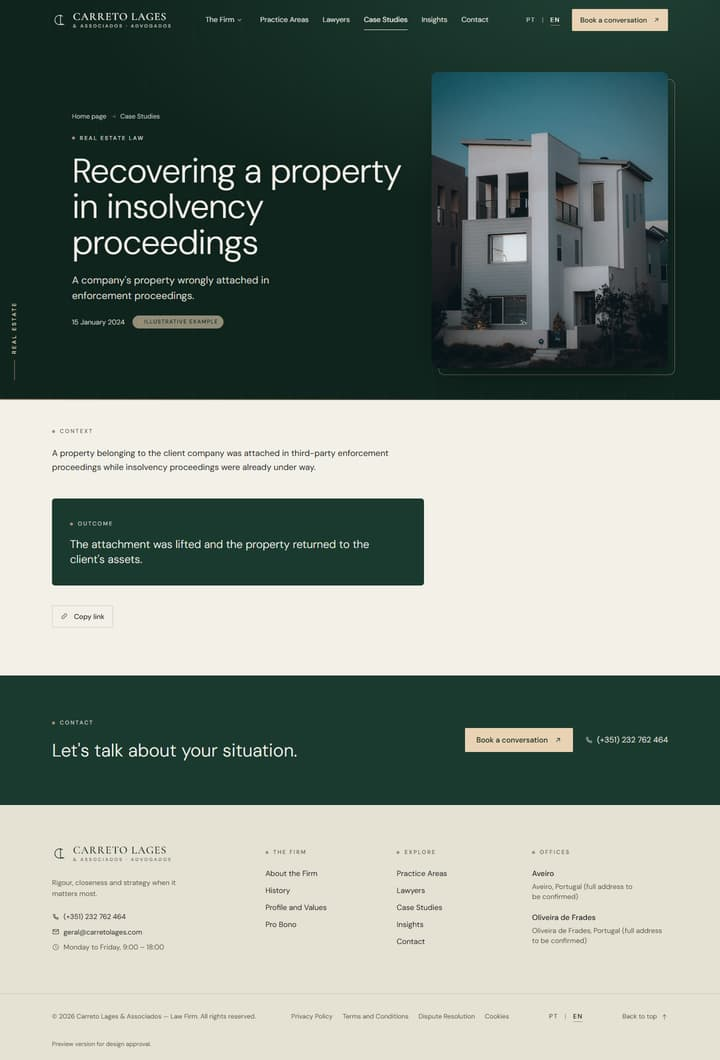
\includegraphics[width=0.485\textwidth]{screenshots/desktop/en/case-studies--property-recovered-insolvency.jpg}\par\medskip
\noindent{\footnotesize Telemóvel (390\,px)}\par\smallskip
\noindent 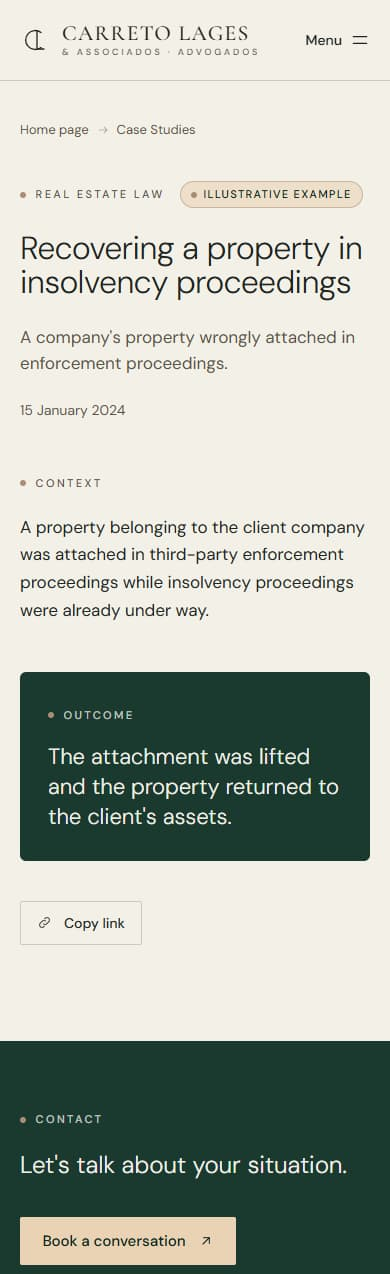
\includegraphics[width=0.235\textwidth]{screenshots/mobile/en/case-studies--property-recovered-insolvency-1.jpg}\hspace{0.012\textwidth}
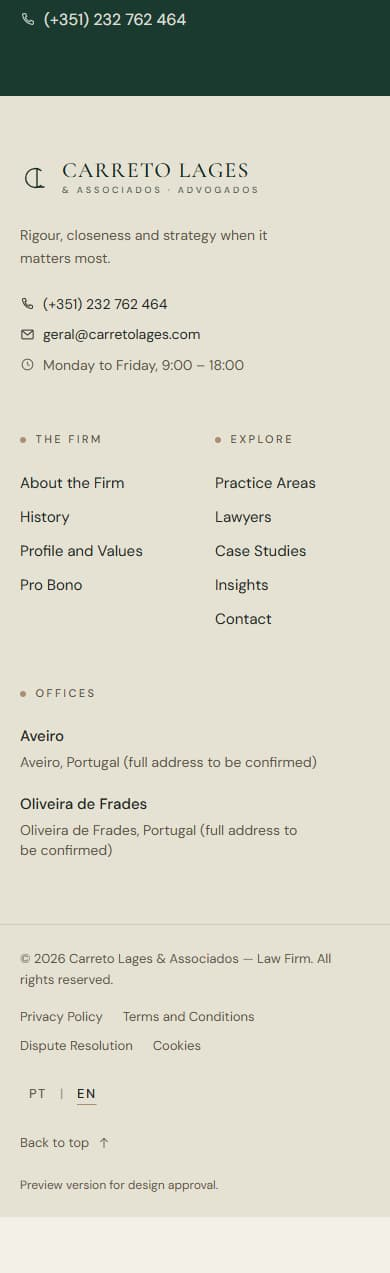
\includegraphics[width=0.235\textwidth]{screenshots/mobile/en/case-studies--property-recovered-insolvency-2.jpg}\par\medskip
\bigskip
\needspace{8\baselineskip}
\subsection*{Talk to us.}
\addcontentsline{toc}{subsection}{Talk to us. (\texttt{/en/contact})}
\noindent{\small\color{tintasuave}\texttt{/en/contact}}\par\smallskip
\noindent{\footnotesize Computador (1440\,px)}\par\smallskip
\noindent 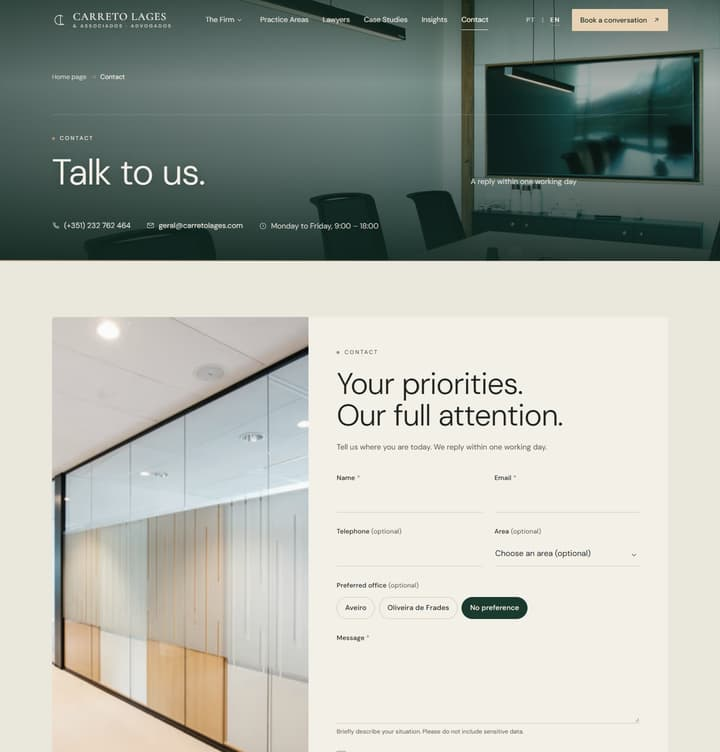
\includegraphics[width=0.485\textwidth]{screenshots/desktop/en/contact-1.jpg}\hspace{0.012\textwidth}
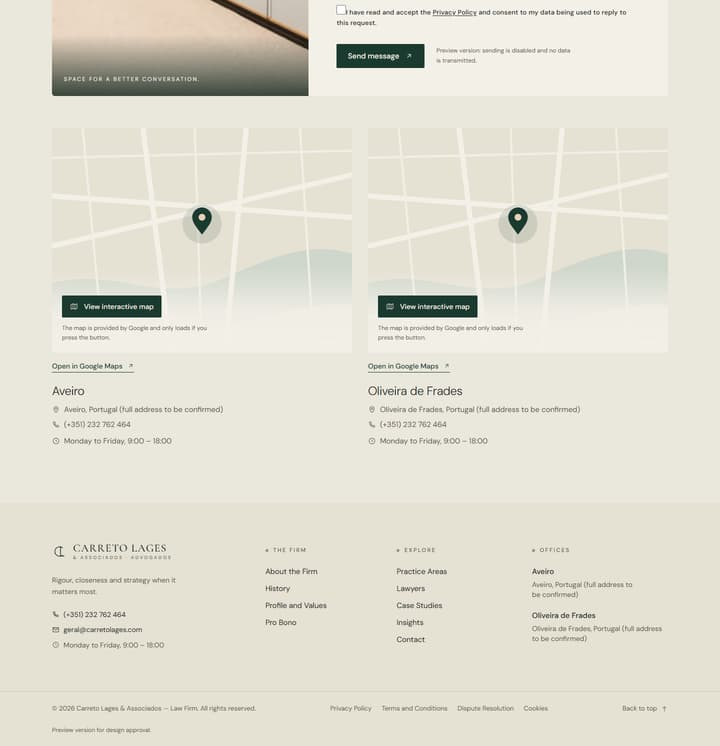
\includegraphics[width=0.485\textwidth]{screenshots/desktop/en/contact-2.jpg}\par\medskip
\noindent{\footnotesize Telemóvel (390\,px)}\par\smallskip
\noindent 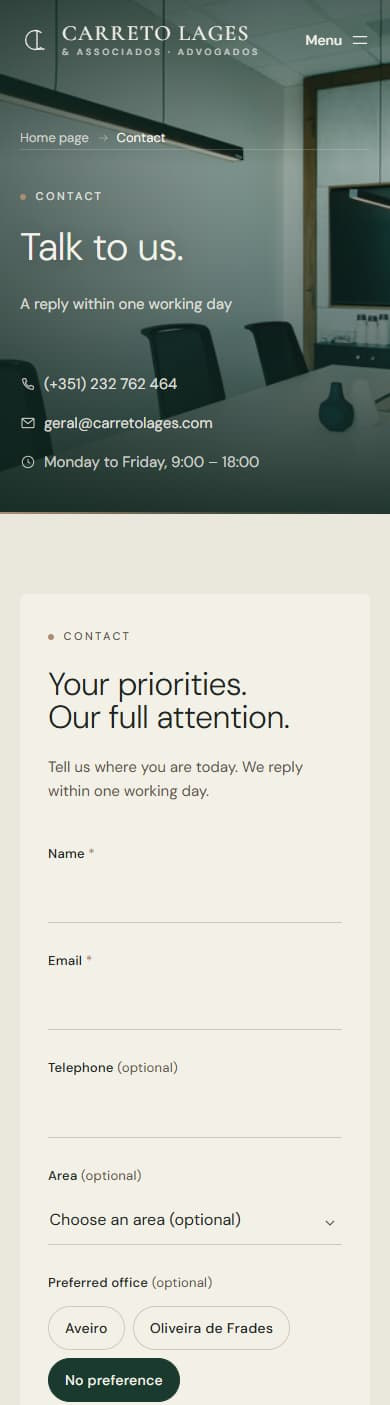
\includegraphics[width=0.235\textwidth]{screenshots/mobile/en/contact-1.jpg}\hspace{0.012\textwidth}
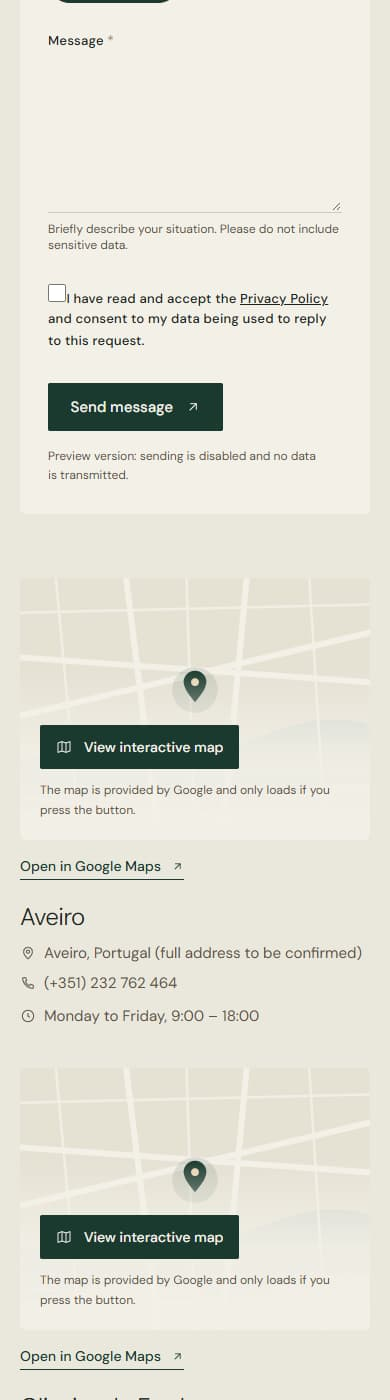
\includegraphics[width=0.235\textwidth]{screenshots/mobile/en/contact-2.jpg}\hspace{0.012\textwidth}
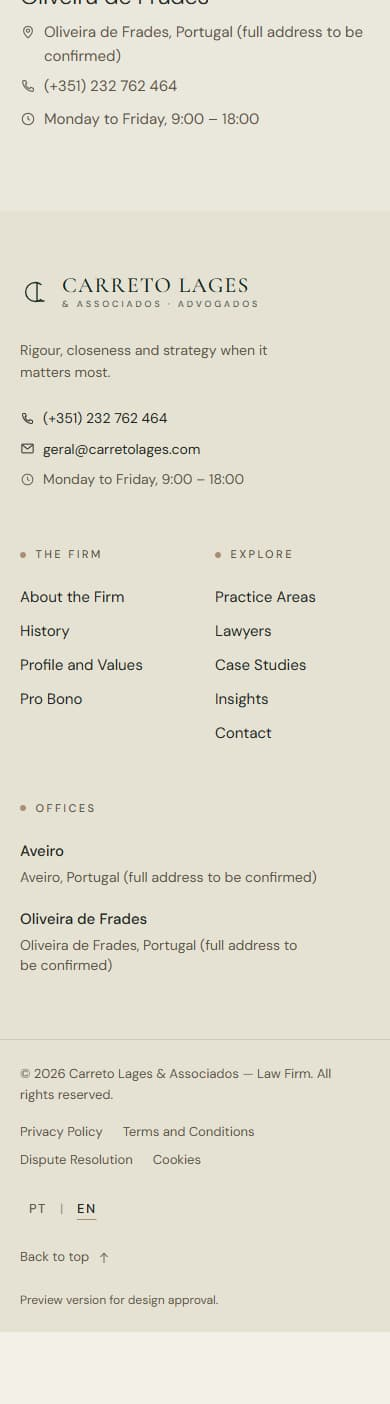
\includegraphics[width=0.235\textwidth]{screenshots/mobile/en/contact-3.jpg}\par\medskip
\bigskip
\needspace{8\baselineskip}
\subsection*{This website does not use cookies.}
\addcontentsline{toc}{subsection}{This website does not use cookies. (\texttt{/en/cookies})}
\noindent{\small\color{tintasuave}\texttt{/en/cookies}}\par\smallskip
\noindent{\footnotesize Computador (1440\,px)}\par\smallskip
\noindent 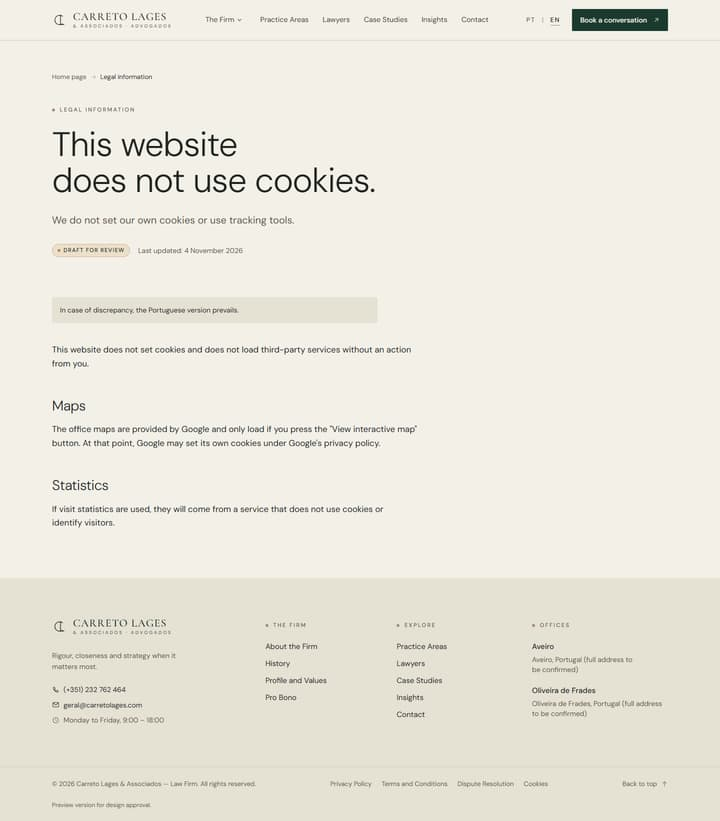
\includegraphics[width=0.485\textwidth]{screenshots/desktop/en/cookies.jpg}\par\medskip
\noindent{\footnotesize Telemóvel (390\,px)}\par\smallskip
\noindent 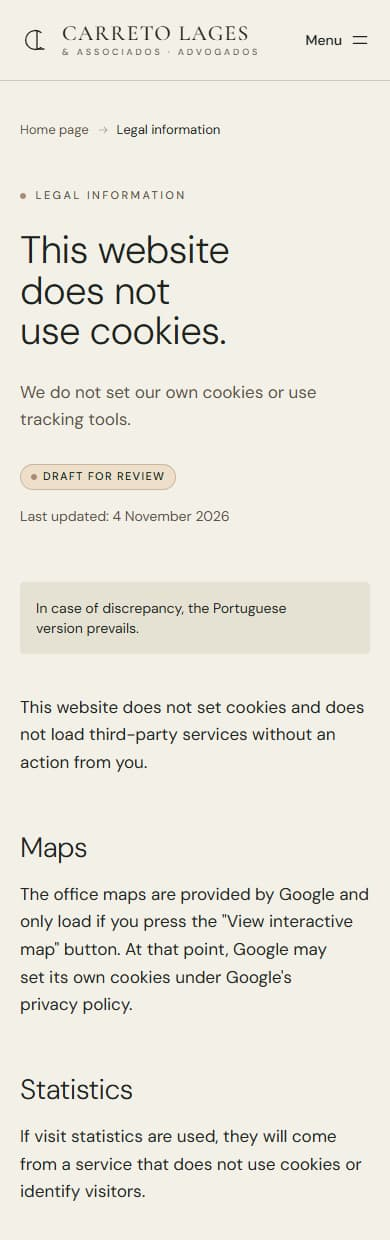
\includegraphics[width=0.235\textwidth]{screenshots/mobile/en/cookies-1.jpg}\hspace{0.012\textwidth}
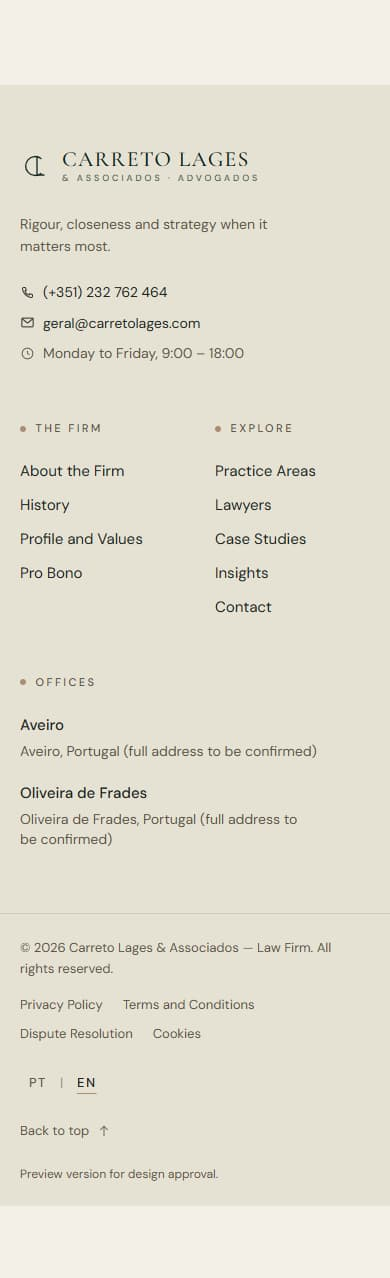
\includegraphics[width=0.235\textwidth]{screenshots/mobile/en/cookies-2.jpg}\par\medskip
\bigskip
\needspace{8\baselineskip}
\subsection*{Dispute Resolution}
\addcontentsline{toc}{subsection}{Dispute Resolution (\texttt{/en/dispute-resolution})}
\noindent{\small\color{tintasuave}\texttt{/en/dispute-resolution}}\par\smallskip
\noindent{\footnotesize Computador (1440\,px)}\par\smallskip
\noindent 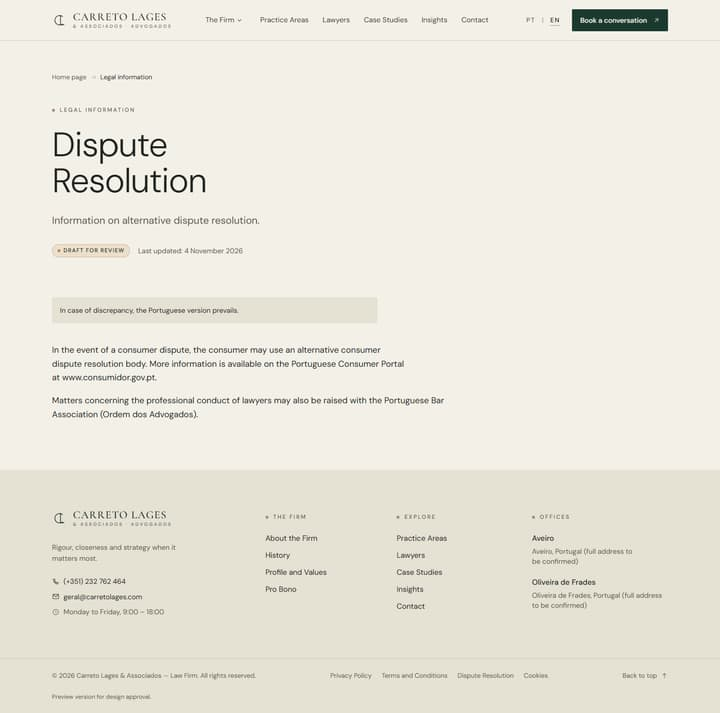
\includegraphics[width=0.485\textwidth]{screenshots/desktop/en/dispute-resolution.jpg}\par\medskip
\noindent{\footnotesize Telemóvel (390\,px)}\par\smallskip
\noindent 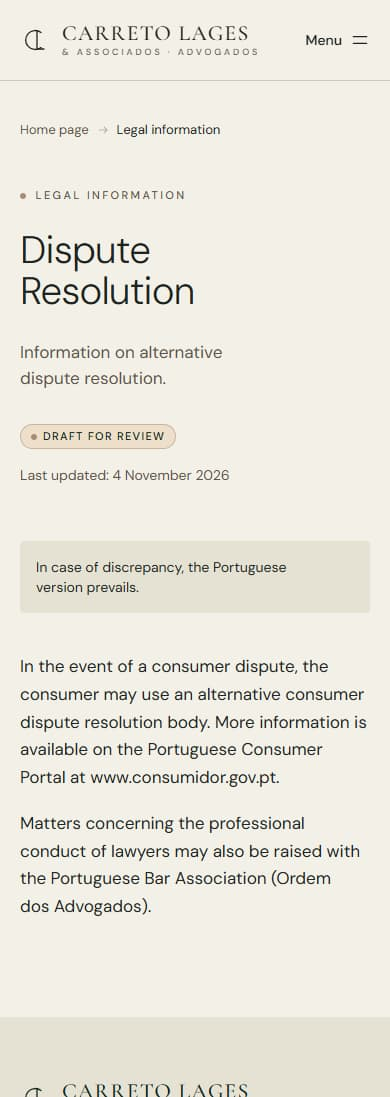
\includegraphics[width=0.235\textwidth]{screenshots/mobile/en/dispute-resolution-1.jpg}\hspace{0.012\textwidth}
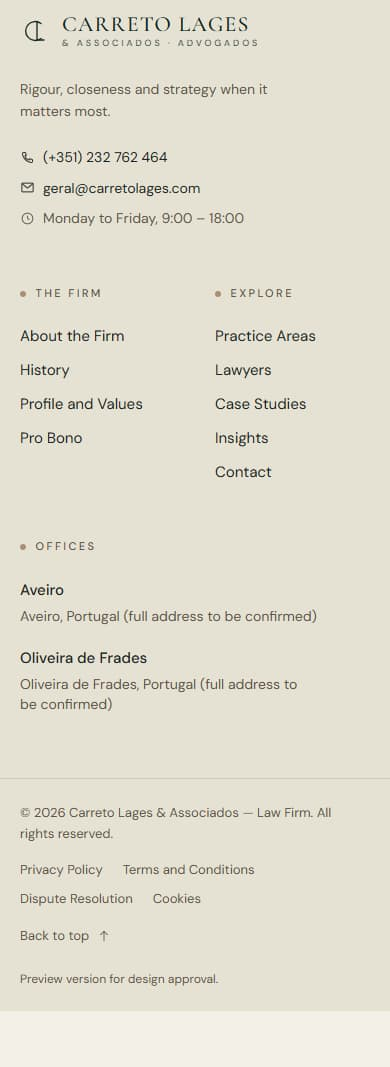
\includegraphics[width=0.235\textwidth]{screenshots/mobile/en/dispute-resolution-2.jpg}\par\medskip
\bigskip
\needspace{8\baselineskip}
\subsection*{Clear notes on what is changing.}
\addcontentsline{toc}{subsection}{Clear notes on what is changing. (\texttt{/en/insights})}
\noindent{\small\color{tintasuave}\texttt{/en/insights}}\par\smallskip
\noindent{\footnotesize Computador (1440\,px)}\par\smallskip
\noindent 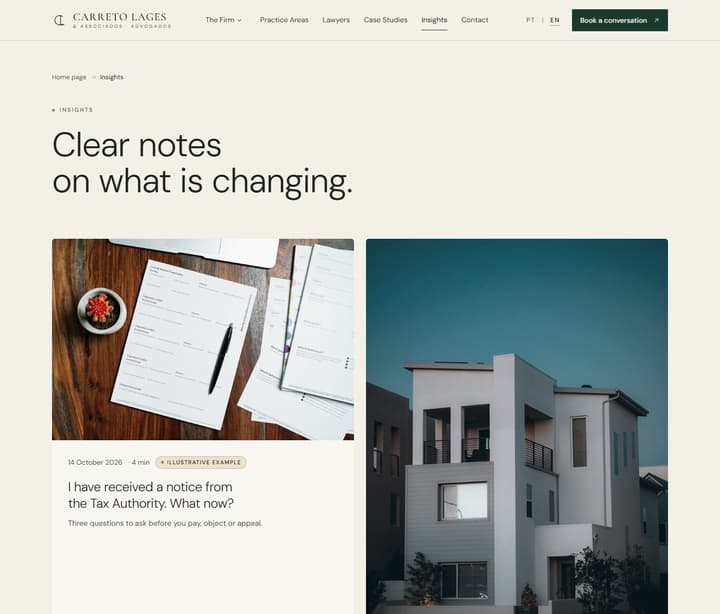
\includegraphics[width=0.485\textwidth]{screenshots/desktop/en/insights-1.jpg}\hspace{0.012\textwidth}
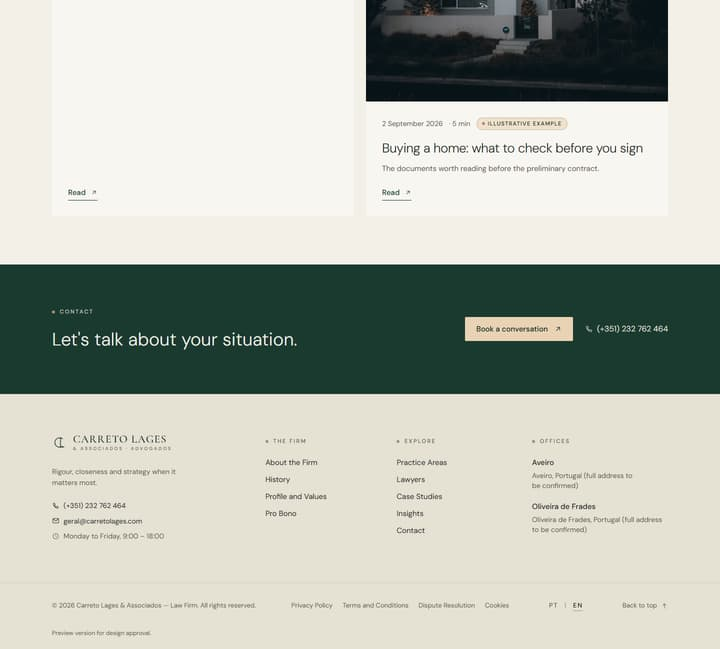
\includegraphics[width=0.485\textwidth]{screenshots/desktop/en/insights-2.jpg}\par\medskip
\noindent{\footnotesize Telemóvel (390\,px)}\par\smallskip
\noindent 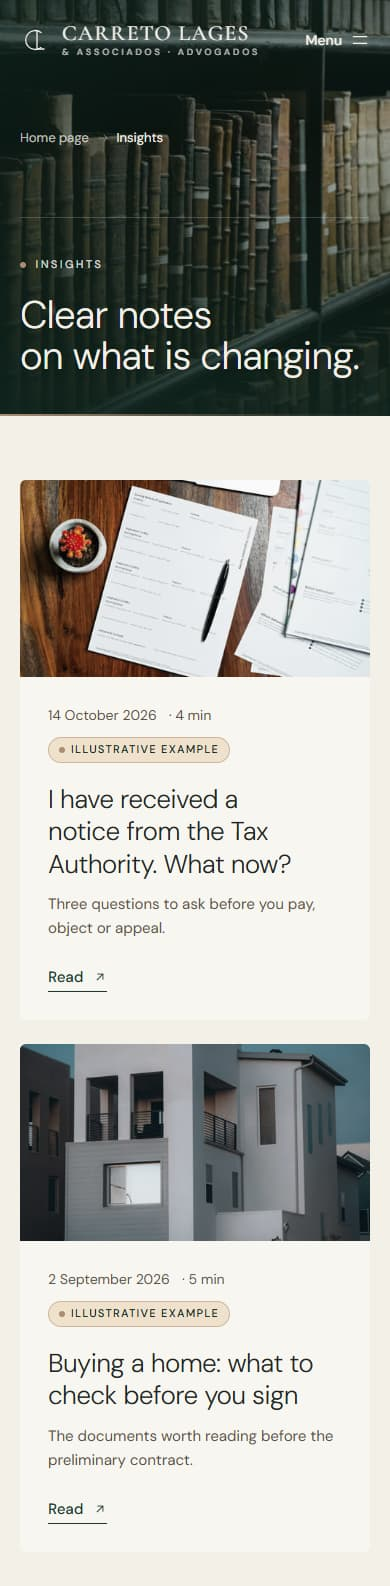
\includegraphics[width=0.235\textwidth]{screenshots/mobile/en/insights-1.jpg}\hspace{0.012\textwidth}
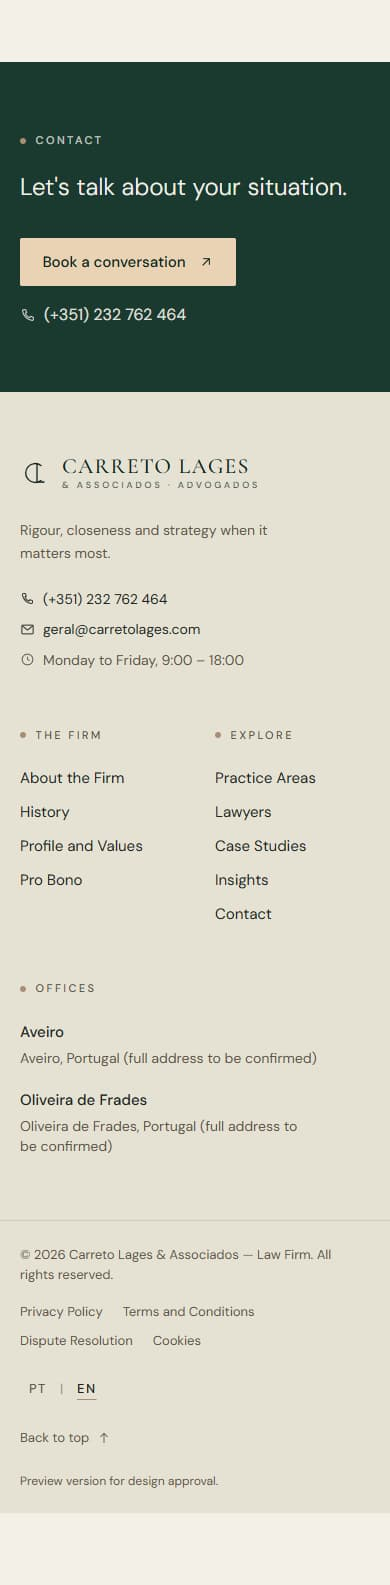
\includegraphics[width=0.235\textwidth]{screenshots/mobile/en/insights-2.jpg}\hspace{0.012\textwidth}
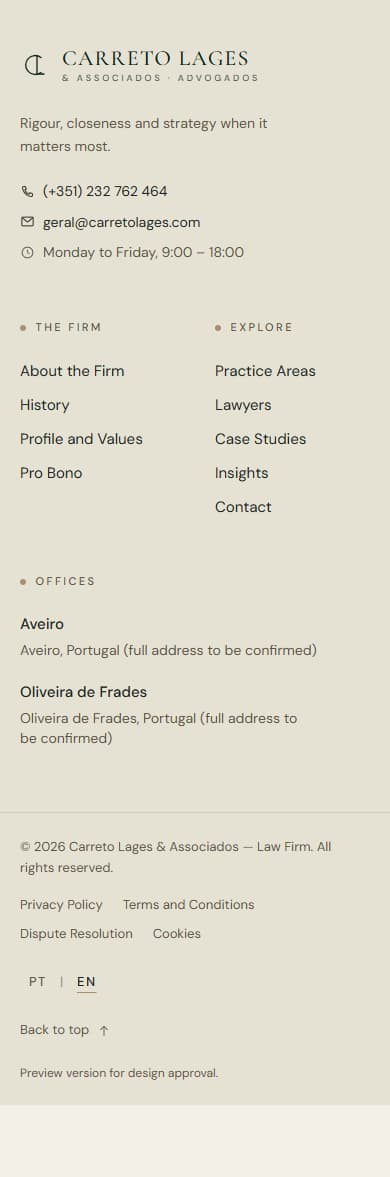
\includegraphics[width=0.235\textwidth]{screenshots/mobile/en/insights-3.jpg}\par\medskip
\bigskip
\needspace{8\baselineskip}
\subsection*{Buying a home: what to check before you sign}
\addcontentsline{toc}{subsection}{Buying a home: what to check before you sign (\texttt{/en/insights/buying-a-home-before-you-sign})}
\noindent{\small\color{tintasuave}\texttt{/en/insights/buying-a-home-before-you-sign}}\par\smallskip
\noindent{\footnotesize Computador (1440\,px)}\par\smallskip
\noindent 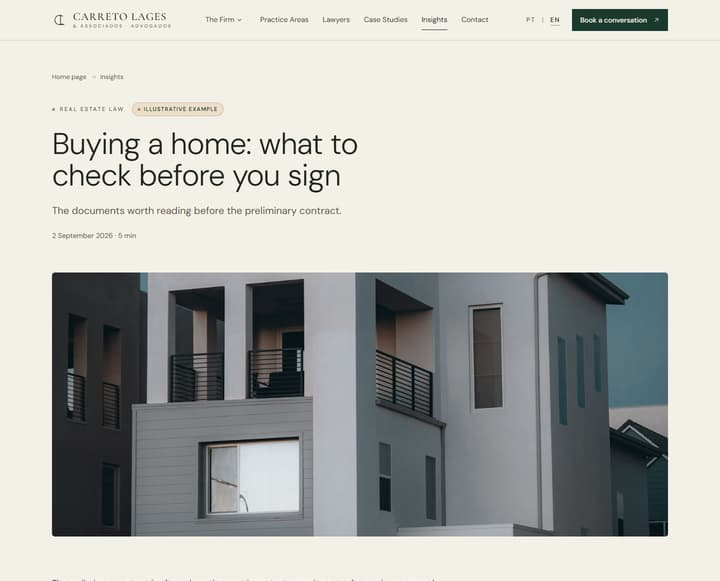
\includegraphics[width=0.485\textwidth]{screenshots/desktop/en/insights--buying-a-home-before-you-sign-1.jpg}\hspace{0.012\textwidth}
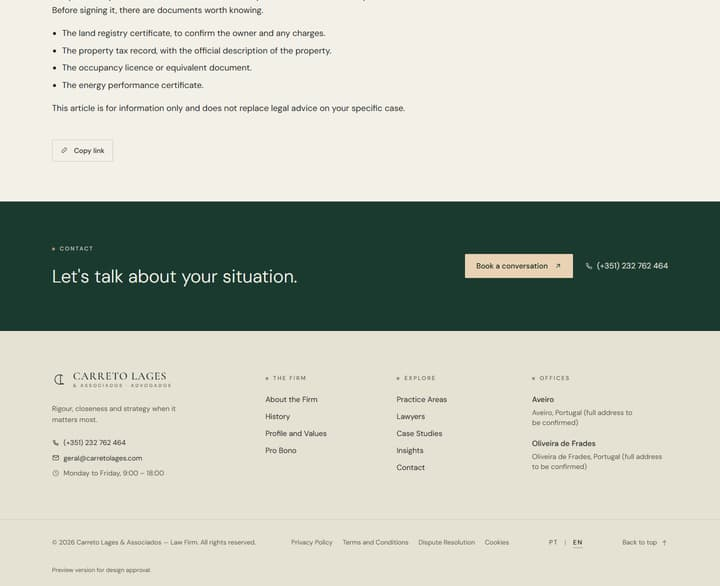
\includegraphics[width=0.485\textwidth]{screenshots/desktop/en/insights--buying-a-home-before-you-sign-2.jpg}\par\medskip
\noindent{\footnotesize Telemóvel (390\,px)}\par\smallskip
\noindent 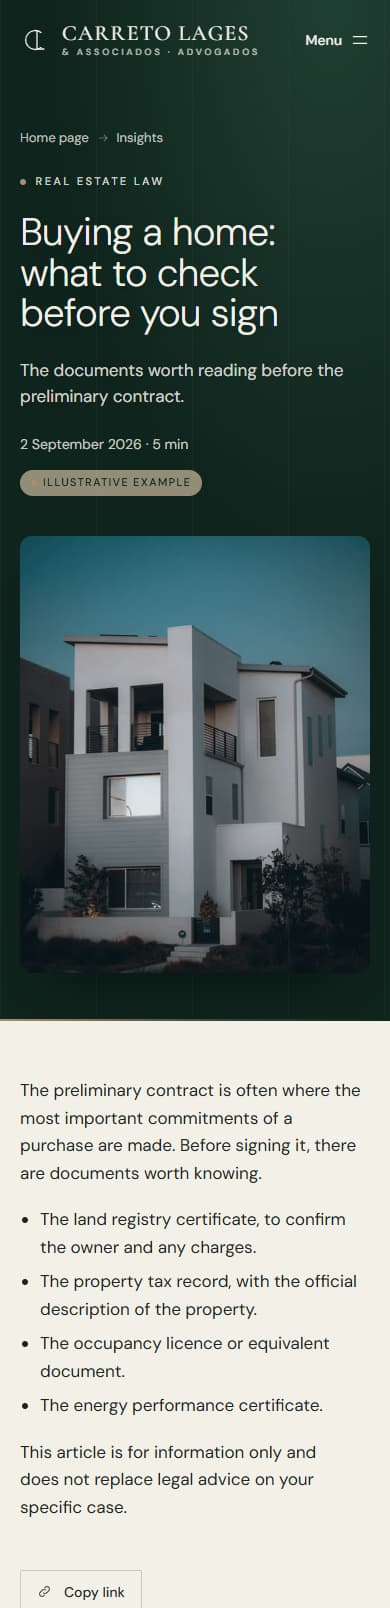
\includegraphics[width=0.235\textwidth]{screenshots/mobile/en/insights--buying-a-home-before-you-sign-1.jpg}\hspace{0.012\textwidth}
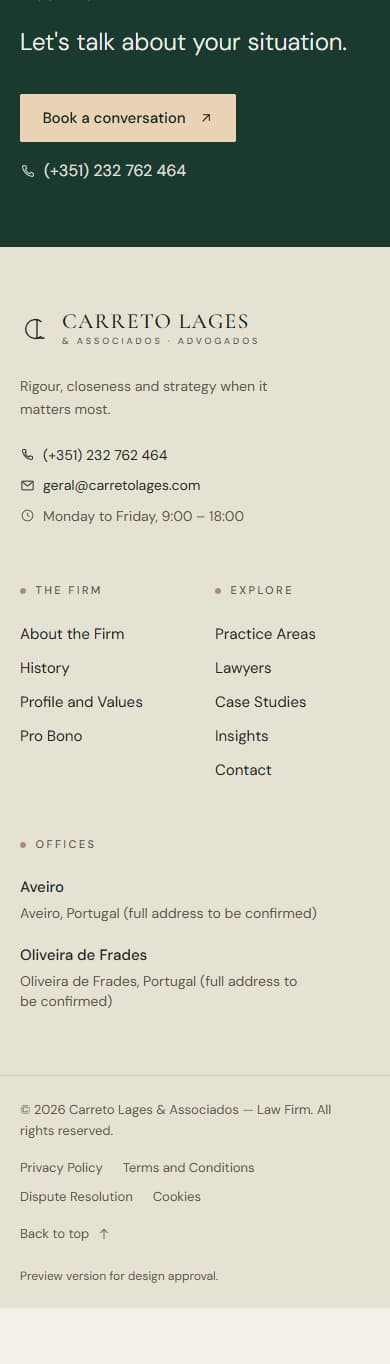
\includegraphics[width=0.235\textwidth]{screenshots/mobile/en/insights--buying-a-home-before-you-sign-2.jpg}\par\medskip
\bigskip
\needspace{8\baselineskip}
\subsection*{I have received a notice from the Tax Authority. What now?}
\addcontentsline{toc}{subsection}{I have received a notice from the Tax Authority. What now? (\texttt{/en/insights/received-a-tax-authority-notice})}
\noindent{\small\color{tintasuave}\texttt{/en/insights/received-a-tax-authority-notice}}\par\smallskip
\noindent{\footnotesize Computador (1440\,px)}\par\smallskip
\noindent 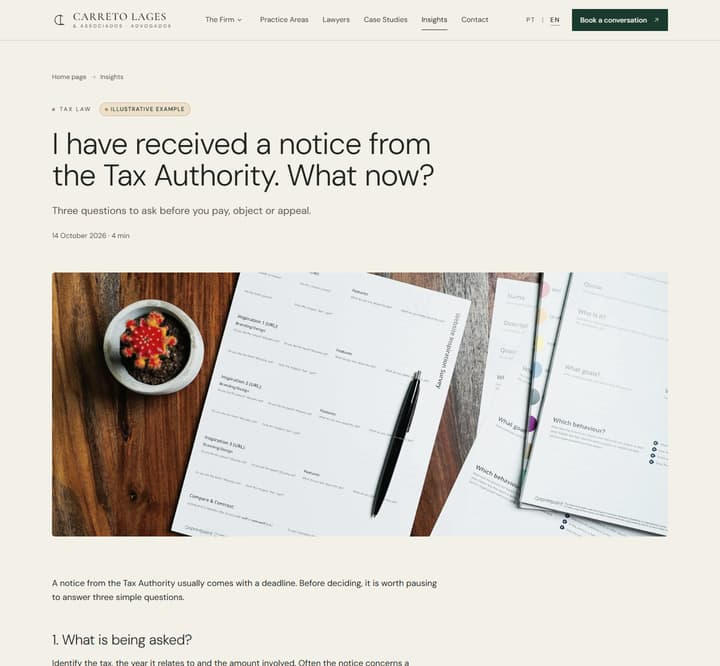
\includegraphics[width=0.485\textwidth]{screenshots/desktop/en/insights--received-a-tax-authority-notice-1.jpg}\hspace{0.012\textwidth}
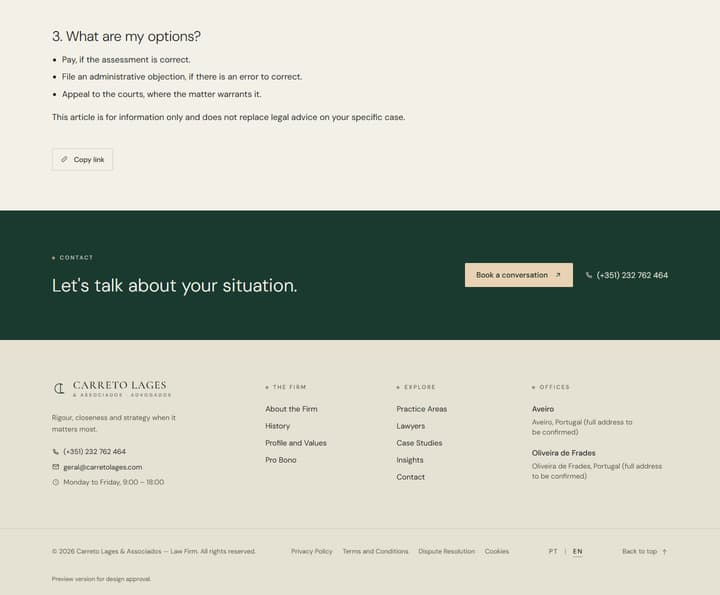
\includegraphics[width=0.485\textwidth]{screenshots/desktop/en/insights--received-a-tax-authority-notice-2.jpg}\par\medskip
\noindent{\footnotesize Telemóvel (390\,px)}\par\smallskip
\noindent 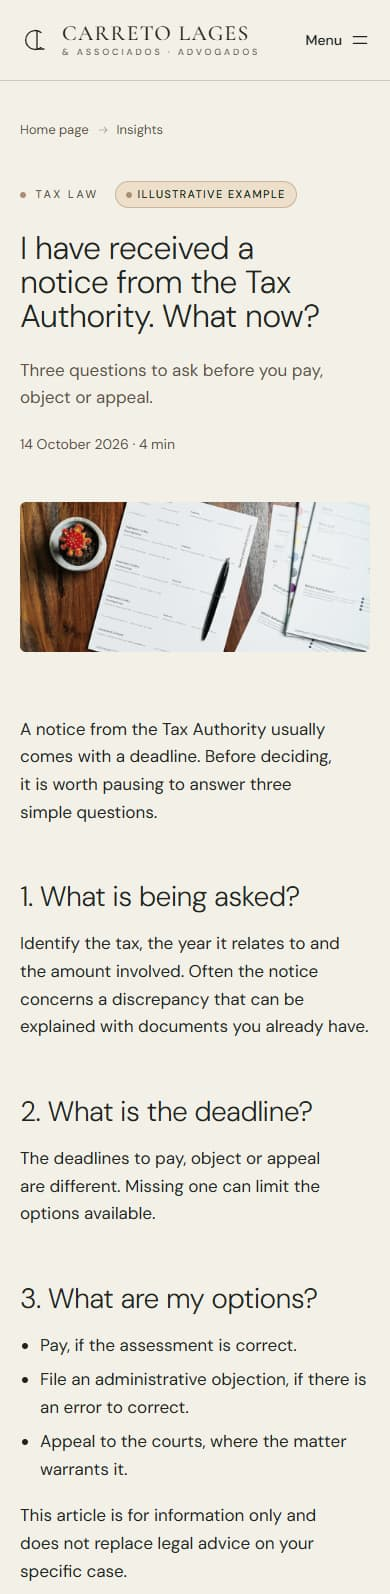
\includegraphics[width=0.235\textwidth]{screenshots/mobile/en/insights--received-a-tax-authority-notice-1.jpg}\hspace{0.012\textwidth}
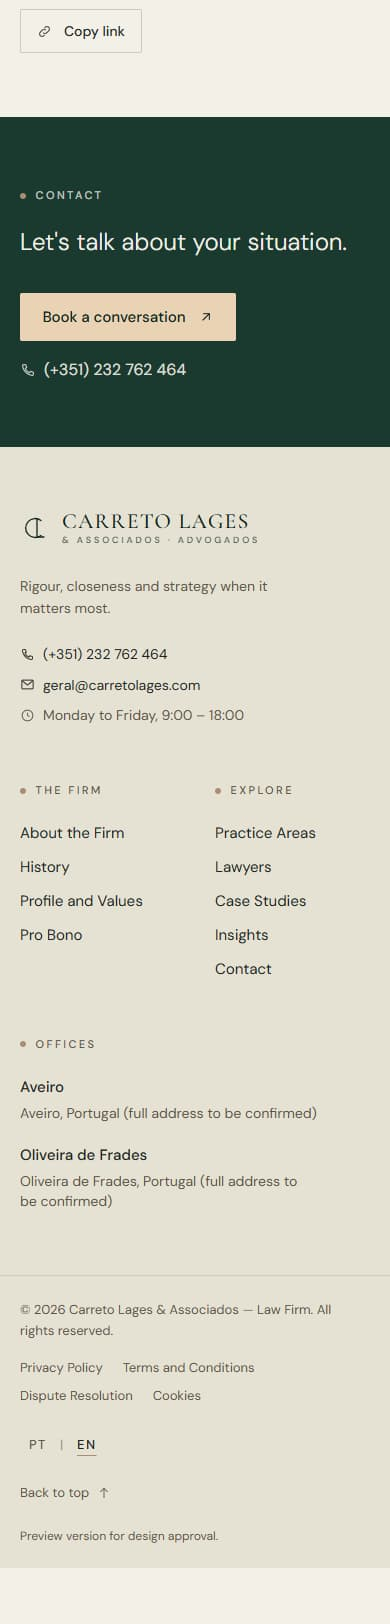
\includegraphics[width=0.235\textwidth]{screenshots/mobile/en/insights--received-a-tax-authority-notice-2.jpg}\par\medskip
\bigskip
\needspace{8\baselineskip}
\subsection*{People you know by name.}
\addcontentsline{toc}{subsection}{People you know by name. (\texttt{/en/lawyers})}
\noindent{\small\color{tintasuave}\texttt{/en/lawyers}}\par\smallskip
\noindent{\footnotesize Computador (1440\,px)}\par\smallskip
\noindent 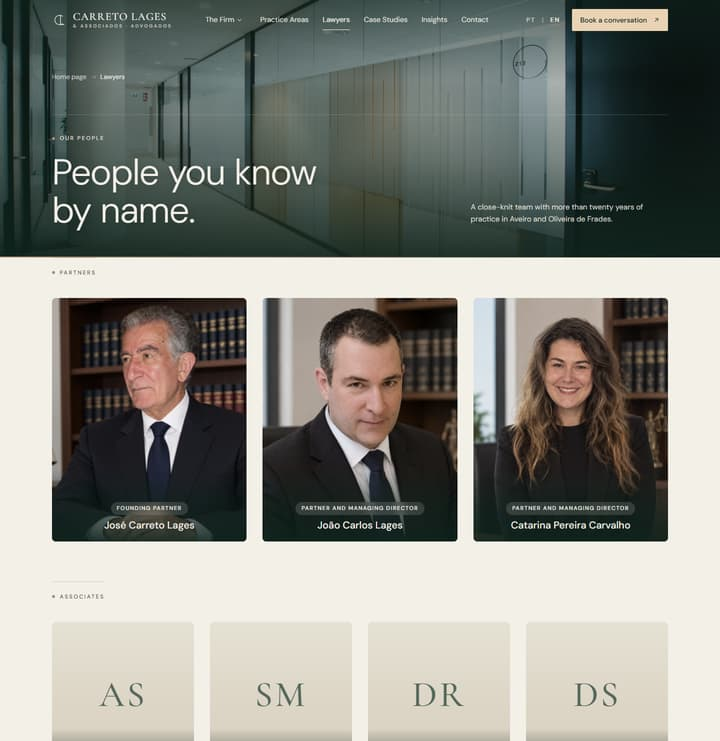
\includegraphics[width=0.485\textwidth]{screenshots/desktop/en/lawyers-1.jpg}\hspace{0.012\textwidth}
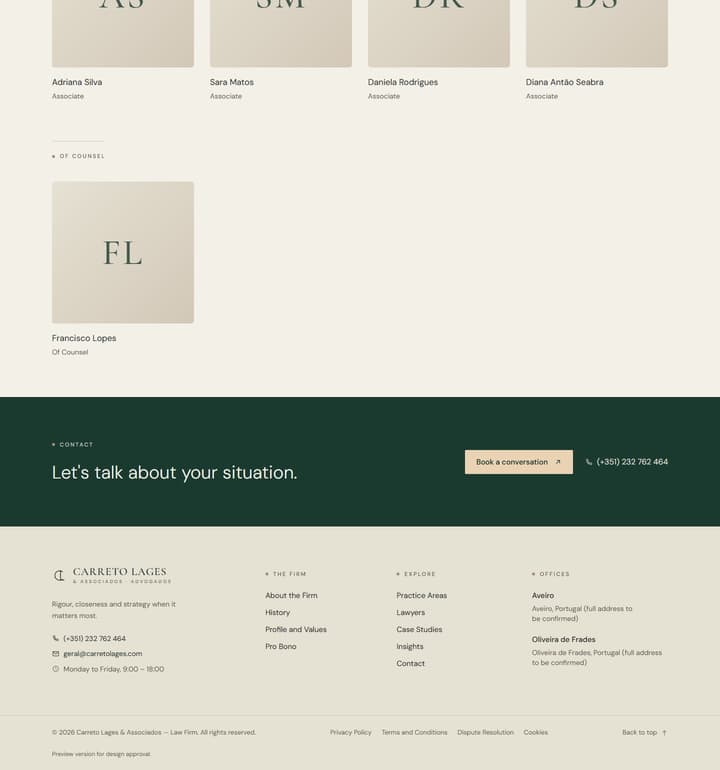
\includegraphics[width=0.485\textwidth]{screenshots/desktop/en/lawyers-2.jpg}\par\medskip
\noindent{\footnotesize Telemóvel (390\,px)}\par\smallskip
\noindent 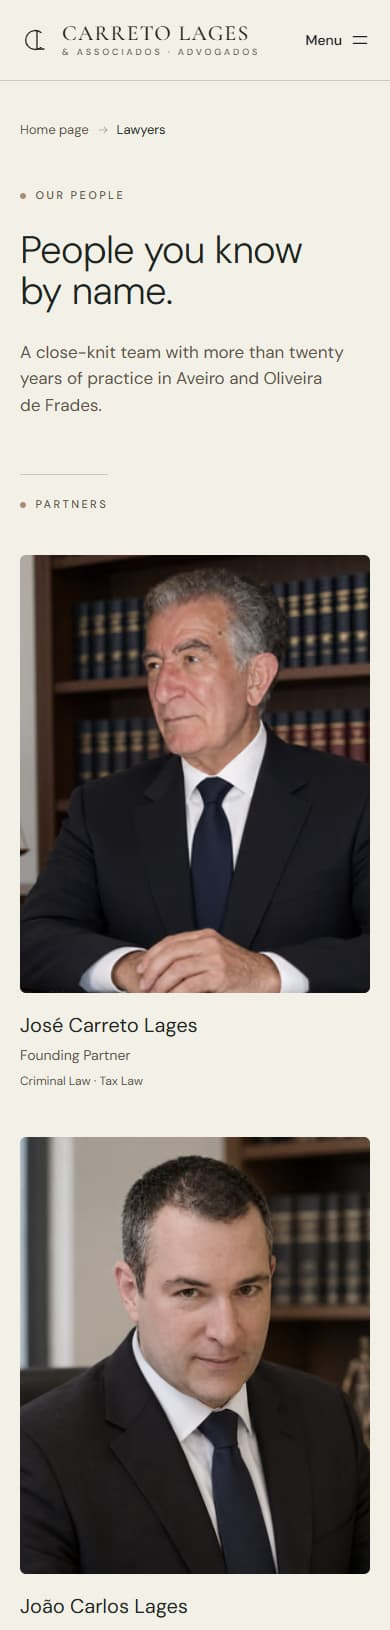
\includegraphics[width=0.235\textwidth]{screenshots/mobile/en/lawyers-1.jpg}\hspace{0.012\textwidth}

\includegraphics[width=0.235\textwidth]{screenshots/mobile/en/lawyers-2.jpg}\hspace{0.012\textwidth}
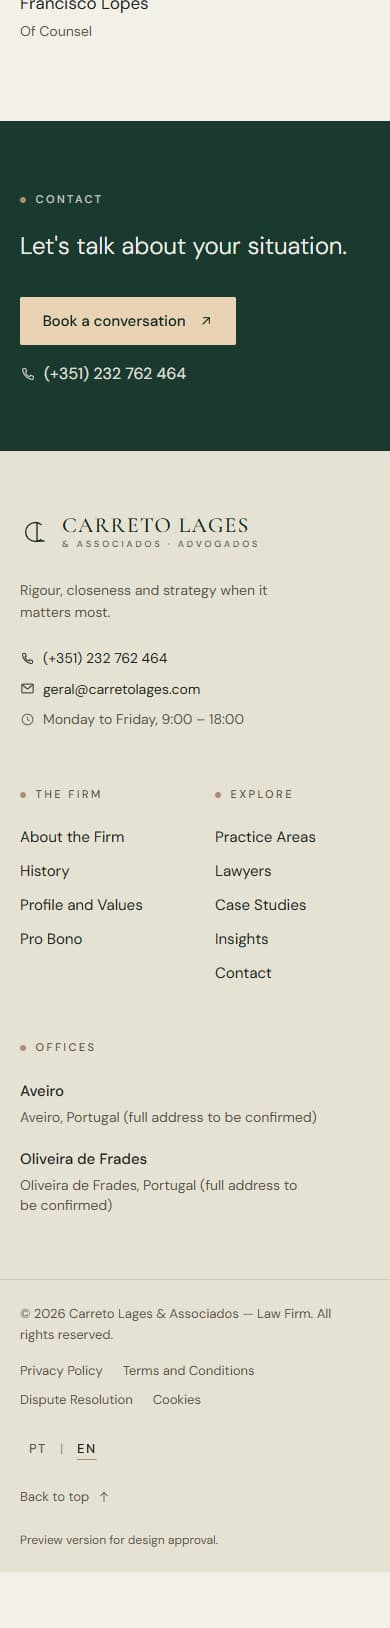
\includegraphics[width=0.235\textwidth]{screenshots/mobile/en/lawyers-3.jpg}\par\medskip
\bigskip
\needspace{8\baselineskip}
\subsection*{Adriana Silva}
\addcontentsline{toc}{subsection}{Adriana Silva (\texttt{/en/lawyers/adriana-silva})}
\noindent{\small\color{tintasuave}\texttt{/en/lawyers/adriana-silva}}\par\smallskip
\noindent{\footnotesize Computador (1440\,px)}\par\smallskip
\noindent 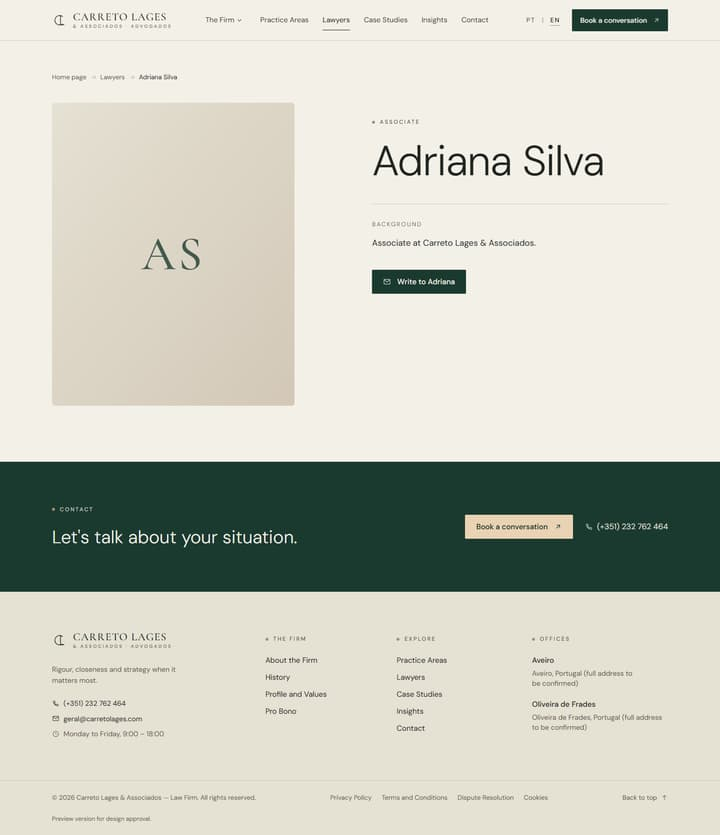
\includegraphics[width=0.485\textwidth]{screenshots/desktop/en/lawyers--adriana-silva.jpg}\par\medskip
\noindent{\footnotesize Telemóvel (390\,px)}\par\smallskip
\noindent 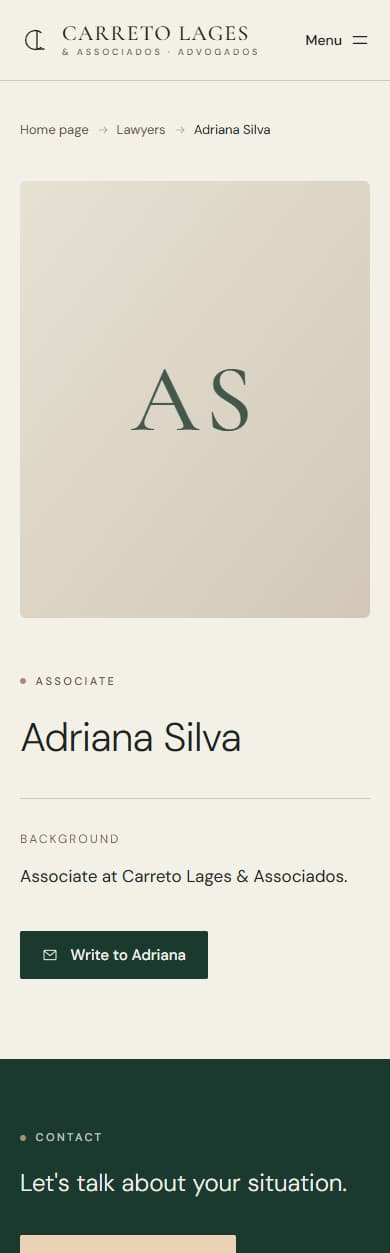
\includegraphics[width=0.235\textwidth]{screenshots/mobile/en/lawyers--adriana-silva-1.jpg}\hspace{0.012\textwidth}
\includegraphics[width=0.235\textwidth]{screenshots/mobile/en/lawyers--adriana-silva-2.jpg}\par\medskip
\bigskip
\needspace{8\baselineskip}
\subsection*{Catarina Pereira Carvalho}
\addcontentsline{toc}{subsection}{Catarina Pereira Carvalho (\texttt{/en/lawyers/catarina-pereira-carvalho})}
\noindent{\small\color{tintasuave}\texttt{/en/lawyers/catarina-pereira-carvalho}}\par\smallskip
\noindent{\footnotesize Computador (1440\,px)}\par\smallskip
\noindent \includegraphics[width=0.485\textwidth]{screenshots/desktop/en/lawyers--catarina-pereira-carvalho.jpg}\par\medskip
\noindent{\footnotesize Telemóvel (390\,px)}\par\smallskip
\noindent \includegraphics[width=0.235\textwidth]{screenshots/mobile/en/lawyers--catarina-pereira-carvalho-1.jpg}\hspace{0.012\textwidth}
\includegraphics[width=0.235\textwidth]{screenshots/mobile/en/lawyers--catarina-pereira-carvalho-2.jpg}\par\medskip
\bigskip
\needspace{8\baselineskip}
\subsection*{Daniela Rodrigues}
\addcontentsline{toc}{subsection}{Daniela Rodrigues (\texttt{/en/lawyers/daniela-rodrigues})}
\noindent{\small\color{tintasuave}\texttt{/en/lawyers/daniela-rodrigues}}\par\smallskip
\noindent{\footnotesize Computador (1440\,px)}\par\smallskip
\noindent \includegraphics[width=0.485\textwidth]{screenshots/desktop/en/lawyers--daniela-rodrigues.jpg}\par\medskip
\noindent{\footnotesize Telemóvel (390\,px)}\par\smallskip
\noindent \includegraphics[width=0.235\textwidth]{screenshots/mobile/en/lawyers--daniela-rodrigues-1.jpg}\hspace{0.012\textwidth}
\includegraphics[width=0.235\textwidth]{screenshots/mobile/en/lawyers--daniela-rodrigues-2.jpg}\par\medskip
\bigskip
\needspace{8\baselineskip}
\subsection*{Diana Antão Seabra}
\addcontentsline{toc}{subsection}{Diana Antão Seabra (\texttt{/en/lawyers/diana-antao-seabra})}
\noindent{\small\color{tintasuave}\texttt{/en/lawyers/diana-antao-seabra}}\par\smallskip
\noindent{\footnotesize Computador (1440\,px)}\par\smallskip
\noindent \includegraphics[width=0.485\textwidth]{screenshots/desktop/en/lawyers--diana-antao-seabra.jpg}\par\medskip
\noindent{\footnotesize Telemóvel (390\,px)}\par\smallskip
\noindent \includegraphics[width=0.235\textwidth]{screenshots/mobile/en/lawyers--diana-antao-seabra-1.jpg}\hspace{0.012\textwidth}
\includegraphics[width=0.235\textwidth]{screenshots/mobile/en/lawyers--diana-antao-seabra-2.jpg}\par\medskip
\bigskip
\needspace{8\baselineskip}
\subsection*{Francisco Lopes}
\addcontentsline{toc}{subsection}{Francisco Lopes (\texttt{/en/lawyers/francisco-lopes})}
\noindent{\small\color{tintasuave}\texttt{/en/lawyers/francisco-lopes}}\par\smallskip
\noindent{\footnotesize Computador (1440\,px)}\par\smallskip
\noindent \includegraphics[width=0.485\textwidth]{screenshots/desktop/en/lawyers--francisco-lopes.jpg}\par\medskip
\noindent{\footnotesize Telemóvel (390\,px)}\par\smallskip
\noindent \includegraphics[width=0.235\textwidth]{screenshots/mobile/en/lawyers--francisco-lopes-1.jpg}\hspace{0.012\textwidth}
\includegraphics[width=0.235\textwidth]{screenshots/mobile/en/lawyers--francisco-lopes-2.jpg}\par\medskip
\bigskip
\needspace{8\baselineskip}
\subsection*{João Carlos Lages}
\addcontentsline{toc}{subsection}{João Carlos Lages (\texttt{/en/lawyers/joao-carlos-lages})}
\noindent{\small\color{tintasuave}\texttt{/en/lawyers/joao-carlos-lages}}\par\smallskip
\noindent{\footnotesize Computador (1440\,px)}\par\smallskip
\noindent \includegraphics[width=0.485\textwidth]{screenshots/desktop/en/lawyers--joao-carlos-lages.jpg}\par\medskip
\noindent{\footnotesize Telemóvel (390\,px)}\par\smallskip
\noindent \includegraphics[width=0.235\textwidth]{screenshots/mobile/en/lawyers--joao-carlos-lages-1.jpg}\hspace{0.012\textwidth}
\includegraphics[width=0.235\textwidth]{screenshots/mobile/en/lawyers--joao-carlos-lages-2.jpg}\par\medskip
\bigskip
\needspace{8\baselineskip}
\subsection*{José Carreto Lages}
\addcontentsline{toc}{subsection}{José Carreto Lages (\texttt{/en/lawyers/jose-carreto-lages})}
\noindent{\small\color{tintasuave}\texttt{/en/lawyers/jose-carreto-lages}}\par\smallskip
\noindent{\footnotesize Computador (1440\,px)}\par\smallskip
\noindent \includegraphics[width=0.485\textwidth]{screenshots/desktop/en/lawyers--jose-carreto-lages.jpg}\par\medskip
\noindent{\footnotesize Telemóvel (390\,px)}\par\smallskip
\noindent \includegraphics[width=0.235\textwidth]{screenshots/mobile/en/lawyers--jose-carreto-lages-1.jpg}\hspace{0.012\textwidth}
\includegraphics[width=0.235\textwidth]{screenshots/mobile/en/lawyers--jose-carreto-lages-2.jpg}\par\medskip
\bigskip
\needspace{8\baselineskip}
\subsection*{Sara Matos}
\addcontentsline{toc}{subsection}{Sara Matos (\texttt{/en/lawyers/sara-matos})}
\noindent{\small\color{tintasuave}\texttt{/en/lawyers/sara-matos}}\par\smallskip
\noindent{\footnotesize Computador (1440\,px)}\par\smallskip
\noindent \includegraphics[width=0.485\textwidth]{screenshots/desktop/en/lawyers--sara-matos.jpg}\par\medskip
\noindent{\footnotesize Telemóvel (390\,px)}\par\smallskip
\noindent \includegraphics[width=0.235\textwidth]{screenshots/mobile/en/lawyers--sara-matos-1.jpg}\hspace{0.012\textwidth}
\includegraphics[width=0.235\textwidth]{screenshots/mobile/en/lawyers--sara-matos-2.jpg}\par\medskip
\bigskip
\needspace{8\baselineskip}
\subsection*{Experience for what comes next.}
\addcontentsline{toc}{subsection}{Experience for what comes next. (\texttt{/en/practice-areas})}
\noindent{\small\color{tintasuave}\texttt{/en/practice-areas}}\par\smallskip
\noindent{\footnotesize Computador (1440\,px)}\par\smallskip
\noindent \includegraphics[width=0.485\textwidth]{screenshots/desktop/en/practice-areas-1.jpg}\hspace{0.012\textwidth}
\includegraphics[width=0.485\textwidth]{screenshots/desktop/en/practice-areas-2.jpg}\par\medskip
\noindent{\footnotesize Telemóvel (390\,px)}\par\smallskip
\noindent \includegraphics[width=0.235\textwidth]{screenshots/mobile/en/practice-areas-1.jpg}\hspace{0.012\textwidth}
\includegraphics[width=0.235\textwidth]{screenshots/mobile/en/practice-areas-2.jpg}\hspace{0.012\textwidth}
\includegraphics[width=0.235\textwidth]{screenshots/mobile/en/practice-areas-3.jpg}\par\medskip
\bigskip
\needspace{8\baselineskip}
\subsection*{Balance in your finances. Strength at the table.}
\addcontentsline{toc}{subsection}{Balance in your finances. Strength at the table. (\texttt{/en/practice-areas/banking-and-finance-law})}
\noindent{\small\color{tintasuave}\texttt{/en/practice-areas/banking-and-finance-law}}\par\smallskip
\noindent{\footnotesize Computador (1440\,px)}\par\smallskip
\noindent \includegraphics[width=0.485\textwidth]{screenshots/desktop/en/practice-areas--banking-and-finance-law-1.jpg}\hspace{0.012\textwidth}
\includegraphics[width=0.485\textwidth]{screenshots/desktop/en/practice-areas--banking-and-finance-law-2.jpg}\par\medskip
\noindent{\footnotesize Telemóvel (390\,px)}\par\smallskip
\noindent \includegraphics[width=0.235\textwidth]{screenshots/mobile/en/practice-areas--banking-and-finance-law-1.jpg}\hspace{0.012\textwidth}
\includegraphics[width=0.235\textwidth]{screenshots/mobile/en/practice-areas--banking-and-finance-law-2.jpg}\hspace{0.012\textwidth}
\includegraphics[width=0.235\textwidth]{screenshots/mobile/en/practice-areas--banking-and-finance-law-3.jpg}\hspace{0.012\textwidth}
\includegraphics[width=0.235\textwidth]{screenshots/mobile/en/practice-areas--banking-and-finance-law-4.jpg}\par\medskip
\bigskip
\needspace{8\baselineskip}
\subsection*{A calm defence. A firm response.}
\addcontentsline{toc}{subsection}{A calm defence. A firm response. (\texttt{/en/practice-areas/criminal-law})}
\noindent{\small\color{tintasuave}\texttt{/en/practice-areas/criminal-law}}\par\smallskip
\noindent{\footnotesize Computador (1440\,px)}\par\smallskip
\noindent \includegraphics[width=0.485\textwidth]{screenshots/desktop/en/practice-areas--criminal-law-1.jpg}\hspace{0.012\textwidth}
\includegraphics[width=0.485\textwidth]{screenshots/desktop/en/practice-areas--criminal-law-2.jpg}\par\medskip
\noindent{\footnotesize Telemóvel (390\,px)}\par\smallskip
\noindent \includegraphics[width=0.235\textwidth]{screenshots/mobile/en/practice-areas--criminal-law-1.jpg}\hspace{0.012\textwidth}
\includegraphics[width=0.235\textwidth]{screenshots/mobile/en/practice-areas--criminal-law-2.jpg}\hspace{0.012\textwidth}
\includegraphics[width=0.235\textwidth]{screenshots/mobile/en/practice-areas--criminal-law-3.jpg}\hspace{0.012\textwidth}
\includegraphics[width=0.235\textwidth]{screenshots/mobile/en/practice-areas--criminal-law-4.jpg}\par\medskip
\bigskip
\needspace{8\baselineskip}
\subsection*{A sound foundation. A wider possibility.}
\addcontentsline{toc}{subsection}{A sound foundation. A wider possibility. (\texttt{/en/practice-areas/real-estate-law})}
\noindent{\small\color{tintasuave}\texttt{/en/practice-areas/real-estate-law}}\par\smallskip
\noindent{\footnotesize Computador (1440\,px)}\par\smallskip
\noindent \includegraphics[width=0.485\textwidth]{screenshots/desktop/en/practice-areas--real-estate-law-1.jpg}\hspace{0.012\textwidth}
\includegraphics[width=0.485\textwidth]{screenshots/desktop/en/practice-areas--real-estate-law-2.jpg}\par\medskip
\noindent{\footnotesize Telemóvel (390\,px)}\par\smallskip
\noindent \includegraphics[width=0.235\textwidth]{screenshots/mobile/en/practice-areas--real-estate-law-1.jpg}\hspace{0.012\textwidth}
\includegraphics[width=0.235\textwidth]{screenshots/mobile/en/practice-areas--real-estate-law-2.jpg}\hspace{0.012\textwidth}
\includegraphics[width=0.235\textwidth]{screenshots/mobile/en/practice-areas--real-estate-law-3.jpg}\hspace{0.012\textwidth}
\includegraphics[width=0.235\textwidth]{screenshots/mobile/en/practice-areas--real-estate-law-4.jpg}\par\medskip
\bigskip
\needspace{8\baselineskip}
\subsection*{Clarity in the numbers. Firmness in the response.}
\addcontentsline{toc}{subsection}{Clarity in the numbers. Firmness in the response. (\texttt{/en/practice-areas/tax-law})}
\noindent{\small\color{tintasuave}\texttt{/en/practice-areas/tax-law}}\par\smallskip
\noindent{\footnotesize Computador (1440\,px)}\par\smallskip
\noindent \includegraphics[width=0.485\textwidth]{screenshots/desktop/en/practice-areas--tax-law-1.jpg}\hspace{0.012\textwidth}
\includegraphics[width=0.485\textwidth]{screenshots/desktop/en/practice-areas--tax-law-2.jpg}\par\medskip
\noindent{\footnotesize Telemóvel (390\,px)}\par\smallskip
\noindent \includegraphics[width=0.235\textwidth]{screenshots/mobile/en/practice-areas--tax-law-1.jpg}\hspace{0.012\textwidth}
\includegraphics[width=0.235\textwidth]{screenshots/mobile/en/practice-areas--tax-law-2.jpg}\hspace{0.012\textwidth}
\includegraphics[width=0.235\textwidth]{screenshots/mobile/en/practice-areas--tax-law-3.jpg}\hspace{0.012\textwidth}
\includegraphics[width=0.235\textwidth]{screenshots/mobile/en/practice-areas--tax-law-4.jpg}\par\medskip
\bigskip
\needspace{8\baselineskip}
\subsection*{Privacy Policy}
\addcontentsline{toc}{subsection}{Privacy Policy (\texttt{/en/privacy-policy})}
\noindent{\small\color{tintasuave}\texttt{/en/privacy-policy}}\par\smallskip
\noindent{\footnotesize Computador (1440\,px)}\par\smallskip
\noindent \includegraphics[width=0.485\textwidth]{screenshots/desktop/en/privacy-policy-1.jpg}\hspace{0.012\textwidth}
\includegraphics[width=0.485\textwidth]{screenshots/desktop/en/privacy-policy-2.jpg}\par\medskip
\noindent{\footnotesize Telemóvel (390\,px)}\par\smallskip
\noindent \includegraphics[width=0.235\textwidth]{screenshots/mobile/en/privacy-policy-1.jpg}\hspace{0.012\textwidth}
\includegraphics[width=0.235\textwidth]{screenshots/mobile/en/privacy-policy-2.jpg}\par\medskip
\bigskip
\needspace{8\baselineskip}
\subsection*{Terms and Conditions}
\addcontentsline{toc}{subsection}{Terms and Conditions (\texttt{/en/terms-and-conditions})}
\noindent{\small\color{tintasuave}\texttt{/en/terms-and-conditions}}\par\smallskip
\noindent{\footnotesize Computador (1440\,px)}\par\smallskip
\noindent \includegraphics[width=0.485\textwidth]{screenshots/desktop/en/terms-and-conditions.jpg}\par\medskip
\noindent{\footnotesize Telemóvel (390\,px)}\par\smallskip
\noindent \includegraphics[width=0.235\textwidth]{screenshots/mobile/en/terms-and-conditions-1.jpg}\hspace{0.012\textwidth}
\includegraphics[width=0.235\textwidth]{screenshots/mobile/en/terms-and-conditions-2.jpg}\par\medskip
\bigskip
\needspace{8\baselineskip}
\subsection*{Thank you. We have received your message.}
\addcontentsline{toc}{subsection}{Thank you. We have received your message. (\texttt{/en/thank-you})}
\noindent{\small\color{tintasuave}\texttt{/en/thank-you}}\par\smallskip
\noindent{\footnotesize Computador (1440\,px)}\par\smallskip
\noindent \includegraphics[width=0.485\textwidth]{screenshots/desktop/en/thank-you.jpg}\par\medskip
\noindent{\footnotesize Telemóvel (390\,px)}\par\smallskip
\noindent \includegraphics[width=0.235\textwidth]{screenshots/mobile/en/thank-you-1.jpg}\hspace{0.012\textwidth}
\includegraphics[width=0.235\textwidth]{screenshots/mobile/en/thank-you-2.jpg}\par\medskip
\bigskip
\needspace{8\baselineskip}
\subsection*{A close-knit firm, since 2002.}
\addcontentsline{toc}{subsection}{A close-knit firm, since 2002. (\texttt{/en/the-firm})}
\noindent{\small\color{tintasuave}\texttt{/en/the-firm}}\par\smallskip
\noindent{\footnotesize Computador (1440\,px)}\par\smallskip
\noindent \includegraphics[width=0.485\textwidth]{screenshots/desktop/en/the-firm.jpg}\par\medskip
\noindent{\footnotesize Telemóvel (390\,px)}\par\smallskip
\noindent \includegraphics[width=0.235\textwidth]{screenshots/mobile/en/the-firm-1.jpg}\hspace{0.012\textwidth}
\includegraphics[width=0.235\textwidth]{screenshots/mobile/en/the-firm-2.jpg}\par\medskip
\bigskip
\needspace{8\baselineskip}
\subsection*{More than two decades alongside our clients.}
\addcontentsline{toc}{subsection}{More than two decades alongside our clients. (\texttt{/en/the-firm/history})}
\noindent{\small\color{tintasuave}\texttt{/en/the-firm/history}}\par\smallskip
\noindent{\footnotesize Computador (1440\,px)}\par\smallskip
\noindent \includegraphics[width=0.485\textwidth]{screenshots/desktop/en/the-firm--history.jpg}\par\medskip
\noindent{\footnotesize Telemóvel (390\,px)}\par\smallskip
\noindent \includegraphics[width=0.235\textwidth]{screenshots/mobile/en/the-firm--history-1.jpg}\hspace{0.012\textwidth}
\includegraphics[width=0.235\textwidth]{screenshots/mobile/en/the-firm--history-2.jpg}\hspace{0.012\textwidth}
\includegraphics[width=0.235\textwidth]{screenshots/mobile/en/the-firm--history-3.jpg}\par\medskip
\bigskip
\needspace{8\baselineskip}
\subsection*{Access to justice is a right.}
\addcontentsline{toc}{subsection}{Access to justice is a right. (\texttt{/en/the-firm/pro-bono})}
\noindent{\small\color{tintasuave}\texttt{/en/the-firm/pro-bono}}\par\smallskip
\noindent{\footnotesize Computador (1440\,px)}\par\smallskip
\noindent \includegraphics[width=0.485\textwidth]{screenshots/desktop/en/the-firm--pro-bono.jpg}\par\medskip
\noindent{\footnotesize Telemóvel (390\,px)}\par\smallskip
\noindent \includegraphics[width=0.235\textwidth]{screenshots/mobile/en/the-firm--pro-bono-1.jpg}\hspace{0.012\textwidth}
\includegraphics[width=0.235\textwidth]{screenshots/mobile/en/the-firm--pro-bono-2.jpg}\par\medskip
\bigskip
\needspace{8\baselineskip}
\subsection*{The principles behind every decision.}
\addcontentsline{toc}{subsection}{The principles behind every decision. (\texttt{/en/the-firm/profile-and-values})}
\noindent{\small\color{tintasuave}\texttt{/en/the-firm/profile-and-values}}\par\smallskip
\noindent{\footnotesize Computador (1440\,px)}\par\smallskip
\noindent \includegraphics[width=0.485\textwidth]{screenshots/desktop/en/the-firm--profile-and-values.jpg}\par\medskip
\noindent{\footnotesize Telemóvel (390\,px)}\par\smallskip
\noindent \includegraphics[width=0.235\textwidth]{screenshots/mobile/en/the-firm--profile-and-values-1.jpg}\hspace{0.012\textwidth}
\includegraphics[width=0.235\textwidth]{screenshots/mobile/en/the-firm--profile-and-values-2.jpg}\hspace{0.012\textwidth}
\includegraphics[width=0.235\textwidth]{screenshots/mobile/en/the-firm--profile-and-values-3.jpg}\par\medskip
\bigskip
\clearpage
\section{Estados e interações — versão portuguesa}
\needspace{8\baselineskip}
\subsection*{Carrossel de áreas no segundo cartão}
\addcontentsline{toc}{subsection}{Carrossel de áreas no segundo cartão (\texttt{/})}
\noindent{\small\color{tintasuave}\texttt{/}}\par\smallskip
\noindent{\footnotesize Computador (1440\,px)}\par\smallskip
\noindent \includegraphics[width=0.9\textwidth]{screenshots/desktop/pt/state-carousel.jpg}\par\medskip
\noindent{\footnotesize Telemóvel (390\,px)}\par\smallskip
\noindent \includegraphics[width=0.3\textwidth]{screenshots/mobile/pt/state-carousel.jpg}\par\medskip
\bigskip
\needspace{8\baselineskip}
\subsection*{Pergunta frequente aberta}
\addcontentsline{toc}{subsection}{Pergunta frequente aberta (\texttt{/})}
\noindent{\small\color{tintasuave}\texttt{/}}\par\smallskip
\noindent{\footnotesize Computador (1440\,px)}\par\smallskip
\noindent \includegraphics[width=0.9\textwidth]{screenshots/desktop/pt/state-faq.jpg}\par\medskip
\noindent{\footnotesize Telemóvel (390\,px)}\par\smallskip
\noindent \includegraphics[width=0.3\textwidth]{screenshots/mobile/pt/state-faq.jpg}\par\medskip
\bigskip
\needspace{8\baselineskip}
\subsection*{Cabeçalho depois de descer na página}
\addcontentsline{toc}{subsection}{Cabeçalho depois de descer na página (\texttt{/})}
\noindent{\small\color{tintasuave}\texttt{/}}\par\smallskip
\noindent{\footnotesize Computador (1440\,px)}\par\smallskip
\noindent \includegraphics[width=0.9\textwidth]{screenshots/desktop/pt/state-header.jpg}\par\medskip
\noindent{\footnotesize Telemóvel (390\,px)}\par\smallskip
\noindent \includegraphics[width=0.3\textwidth]{screenshots/mobile/pt/state-header.jpg}\par\medskip
\bigskip
\needspace{8\baselineskip}
\subsection*{Menu de telemóvel aberto}
\addcontentsline{toc}{subsection}{Menu de telemóvel aberto (\texttt{/})}
\noindent{\small\color{tintasuave}\texttt{/}}\par\smallskip
\noindent{\footnotesize Telemóvel (390\,px)}\par\smallskip
\noindent \includegraphics[width=0.3\textwidth]{screenshots/mobile/pt/state-menu.jpg}\par\medskip
\bigskip
\needspace{8\baselineskip}
\subsection*{``Em que situação está?'' com a terceira situação escolhida}
\addcontentsline{toc}{subsection}{``Em que situação está?'' com a terceira situação escolhida (\texttt{/})}
\noindent{\small\color{tintasuave}\texttt{/}}\par\smallskip
\noindent{\footnotesize Computador (1440\,px)}\par\smallskip
\noindent \includegraphics[width=0.9\textwidth]{screenshots/desktop/pt/state-situation.jpg}\par\medskip
\noindent{\footnotesize Telemóvel (390\,px)}\par\smallskip
\noindent \includegraphics[width=0.3\textwidth]{screenshots/mobile/pt/state-situation.jpg}\par\medskip
\bigskip
\needspace{8\baselineskip}
\subsection*{Vídeo do topo em pausa}
\addcontentsline{toc}{subsection}{Vídeo do topo em pausa (\texttt{/})}
\noindent{\small\color{tintasuave}\texttt{/}}\par\smallskip
\noindent{\footnotesize Computador (1440\,px)}\par\smallskip
\noindent \includegraphics[width=0.9\textwidth]{screenshots/desktop/pt/state-video-paused.jpg}\par\medskip
\noindent{\footnotesize Telemóvel (390\,px)}\par\smallskip
\noindent \includegraphics[width=0.3\textwidth]{screenshots/mobile/pt/state-video-paused.jpg}\par\medskip
\bigskip
\needspace{8\baselineskip}
\subsection*{Formulário com erros de validação}
\addcontentsline{toc}{subsection}{Formulário com erros de validação (\texttt{/contactos})}
\noindent{\small\color{tintasuave}\texttt{/contactos}}\par\smallskip
\noindent{\footnotesize Computador (1440\,px)}\par\smallskip
\noindent \includegraphics[width=0.9\textwidth]{screenshots/desktop/pt/state-form-errors.jpg}\par\medskip
\noindent{\footnotesize Telemóvel (390\,px)}\par\smallskip
\noindent \includegraphics[width=0.3\textwidth]{screenshots/mobile/pt/state-form-errors.jpg}\par\medskip
\bigskip
\needspace{8\baselineskip}
\subsection*{Mapa interativo carregado depois do clique}
\addcontentsline{toc}{subsection}{Mapa interativo carregado depois do clique (\texttt{/contactos})}
\noindent{\small\color{tintasuave}\texttt{/contactos}}\par\smallskip
\noindent{\footnotesize Computador (1440\,px)}\par\smallskip
\noindent \includegraphics[width=0.9\textwidth]{screenshots/desktop/pt/state-map.jpg}\par\medskip
\noindent{\footnotesize Telemóvel (390\,px)}\par\smallskip
\noindent \includegraphics[width=0.3\textwidth]{screenshots/mobile/pt/state-map.jpg}\par\medskip
\bigskip
\clearpage
\section{Estados e interações — versão inglesa}
\needspace{8\baselineskip}
\subsection*{Areas carousel on the second card}
\addcontentsline{toc}{subsection}{Areas carousel on the second card (\texttt{/en})}
\noindent{\small\color{tintasuave}\texttt{/en}}\par\smallskip
\noindent{\footnotesize Computador (1440\,px)}\par\smallskip
\noindent \includegraphics[width=0.9\textwidth]{screenshots/desktop/en/state-carousel.jpg}\par\medskip
\noindent{\footnotesize Telemóvel (390\,px)}\par\smallskip
\noindent \includegraphics[width=0.3\textwidth]{screenshots/mobile/en/state-carousel.jpg}\par\medskip
\bigskip
\needspace{8\baselineskip}
\subsection*{FAQ item open}
\addcontentsline{toc}{subsection}{FAQ item open (\texttt{/en})}
\noindent{\small\color{tintasuave}\texttt{/en}}\par\smallskip
\noindent{\footnotesize Computador (1440\,px)}\par\smallskip
\noindent \includegraphics[width=0.9\textwidth]{screenshots/desktop/en/state-faq.jpg}\par\medskip
\noindent{\footnotesize Telemóvel (390\,px)}\par\smallskip
\noindent \includegraphics[width=0.3\textwidth]{screenshots/mobile/en/state-faq.jpg}\par\medskip
\bigskip
\needspace{8\baselineskip}
\subsection*{Header after scrolling}
\addcontentsline{toc}{subsection}{Header after scrolling (\texttt{/en})}
\noindent{\small\color{tintasuave}\texttt{/en}}\par\smallskip
\noindent{\footnotesize Computador (1440\,px)}\par\smallskip
\noindent \includegraphics[width=0.9\textwidth]{screenshots/desktop/en/state-header.jpg}\par\medskip
\noindent{\footnotesize Telemóvel (390\,px)}\par\smallskip
\noindent \includegraphics[width=0.3\textwidth]{screenshots/mobile/en/state-header.jpg}\par\medskip
\bigskip
\needspace{8\baselineskip}
\subsection*{Mobile menu open}
\addcontentsline{toc}{subsection}{Mobile menu open (\texttt{/en})}
\noindent{\small\color{tintasuave}\texttt{/en}}\par\smallskip
\noindent{\footnotesize Telemóvel (390\,px)}\par\smallskip
\noindent \includegraphics[width=0.3\textwidth]{screenshots/mobile/en/state-menu.jpg}\par\medskip
\bigskip
\needspace{8\baselineskip}
\subsection*{``Where are you today?'' with the third situation selected}
\addcontentsline{toc}{subsection}{``Where are you today?'' with the third situation selected (\texttt{/en})}
\noindent{\small\color{tintasuave}\texttt{/en}}\par\smallskip
\noindent{\footnotesize Computador (1440\,px)}\par\smallskip
\noindent \includegraphics[width=0.9\textwidth]{screenshots/desktop/en/state-situation.jpg}\par\medskip
\noindent{\footnotesize Telemóvel (390\,px)}\par\smallskip
\noindent \includegraphics[width=0.3\textwidth]{screenshots/mobile/en/state-situation.jpg}\par\medskip
\bigskip
\needspace{8\baselineskip}
\subsection*{Hero video paused}
\addcontentsline{toc}{subsection}{Hero video paused (\texttt{/en})}
\noindent{\small\color{tintasuave}\texttt{/en}}\par\smallskip
\noindent{\footnotesize Computador (1440\,px)}\par\smallskip
\noindent \includegraphics[width=0.9\textwidth]{screenshots/desktop/en/state-video-paused.jpg}\par\medskip
\noindent{\footnotesize Telemóvel (390\,px)}\par\smallskip
\noindent \includegraphics[width=0.3\textwidth]{screenshots/mobile/en/state-video-paused.jpg}\par\medskip
\bigskip
\needspace{8\baselineskip}
\subsection*{Form with validation errors}
\addcontentsline{toc}{subsection}{Form with validation errors (\texttt{/en/contact})}
\noindent{\small\color{tintasuave}\texttt{/en/contact}}\par\smallskip
\noindent{\footnotesize Computador (1440\,px)}\par\smallskip
\noindent \includegraphics[width=0.9\textwidth]{screenshots/desktop/en/state-form-errors.jpg}\par\medskip
\noindent{\footnotesize Telemóvel (390\,px)}\par\smallskip
\noindent \includegraphics[width=0.3\textwidth]{screenshots/mobile/en/state-form-errors.jpg}\par\medskip
\bigskip
\needspace{8\baselineskip}
\subsection*{Interactive map loaded after the click}
\addcontentsline{toc}{subsection}{Interactive map loaded after the click (\texttt{/en/contact})}
\noindent{\small\color{tintasuave}\texttt{/en/contact}}\par\smallskip
\noindent{\footnotesize Computador (1440\,px)}\par\smallskip
\noindent \includegraphics[width=0.9\textwidth]{screenshots/desktop/en/state-map.jpg}\par\medskip
\noindent{\footnotesize Telemóvel (390\,px)}\par\smallskip
\noindent \includegraphics[width=0.3\textwidth]{screenshots/mobile/en/state-map.jpg}\par\medskip
\bigskip


\end{document}
